\documentclass [11 pt, oneside] {article}


\def \jtitle {Algebraic geometry}
\def \jlecturer {Richard Borcherds}
\def \jterm {}
\def \jauthor {Jack DeSerrano}


\usepackage [course] {jack}

\title {Algebraic geometry}
\author {Jack DeSerrano}



\begin{document}
\ifams
    \topskip0pt
    \vspace*{\fill}
\fi
\maketitle
\thispagestyle{empty}
These notes are based on some of Richard Borcherds's YouTube series on algebraic geometry. 
Section 1 concerns varieties,\footnote{See \url{https://www.youtube.com/playlist?list=PL8yHsr3EFj53j51FG6wCbQKjBgpjKa5PX}.} 
section 2 concerns schemes,\footnote{See \url{https://www.youtube.com/playlist?list=PL8yHsr3EFj50Un2NpfPySgXctRQK7CLG-}.} 
and sections 3--6 treat miscellaneous topics.\footnote{See \url{https://www.youtube.com/playlist?list=PL8yHsr3EFj53Rwr6ly1oUasJXR2Qerwgj}.} 
Dr. Borcherds refers to Hartshorne's \ul{Algebraic Geometry}.\footnote{See \url{https://link.springer.com/book/10.1007/978-1-4757-3849-0}.} 
I tend to use Grothendieck's EGA. 
Unless stated otherwise, rings are assumed to be commutative.
\hypersetup{linkcolor = black}

\begin{figure}
	\begin{center}
		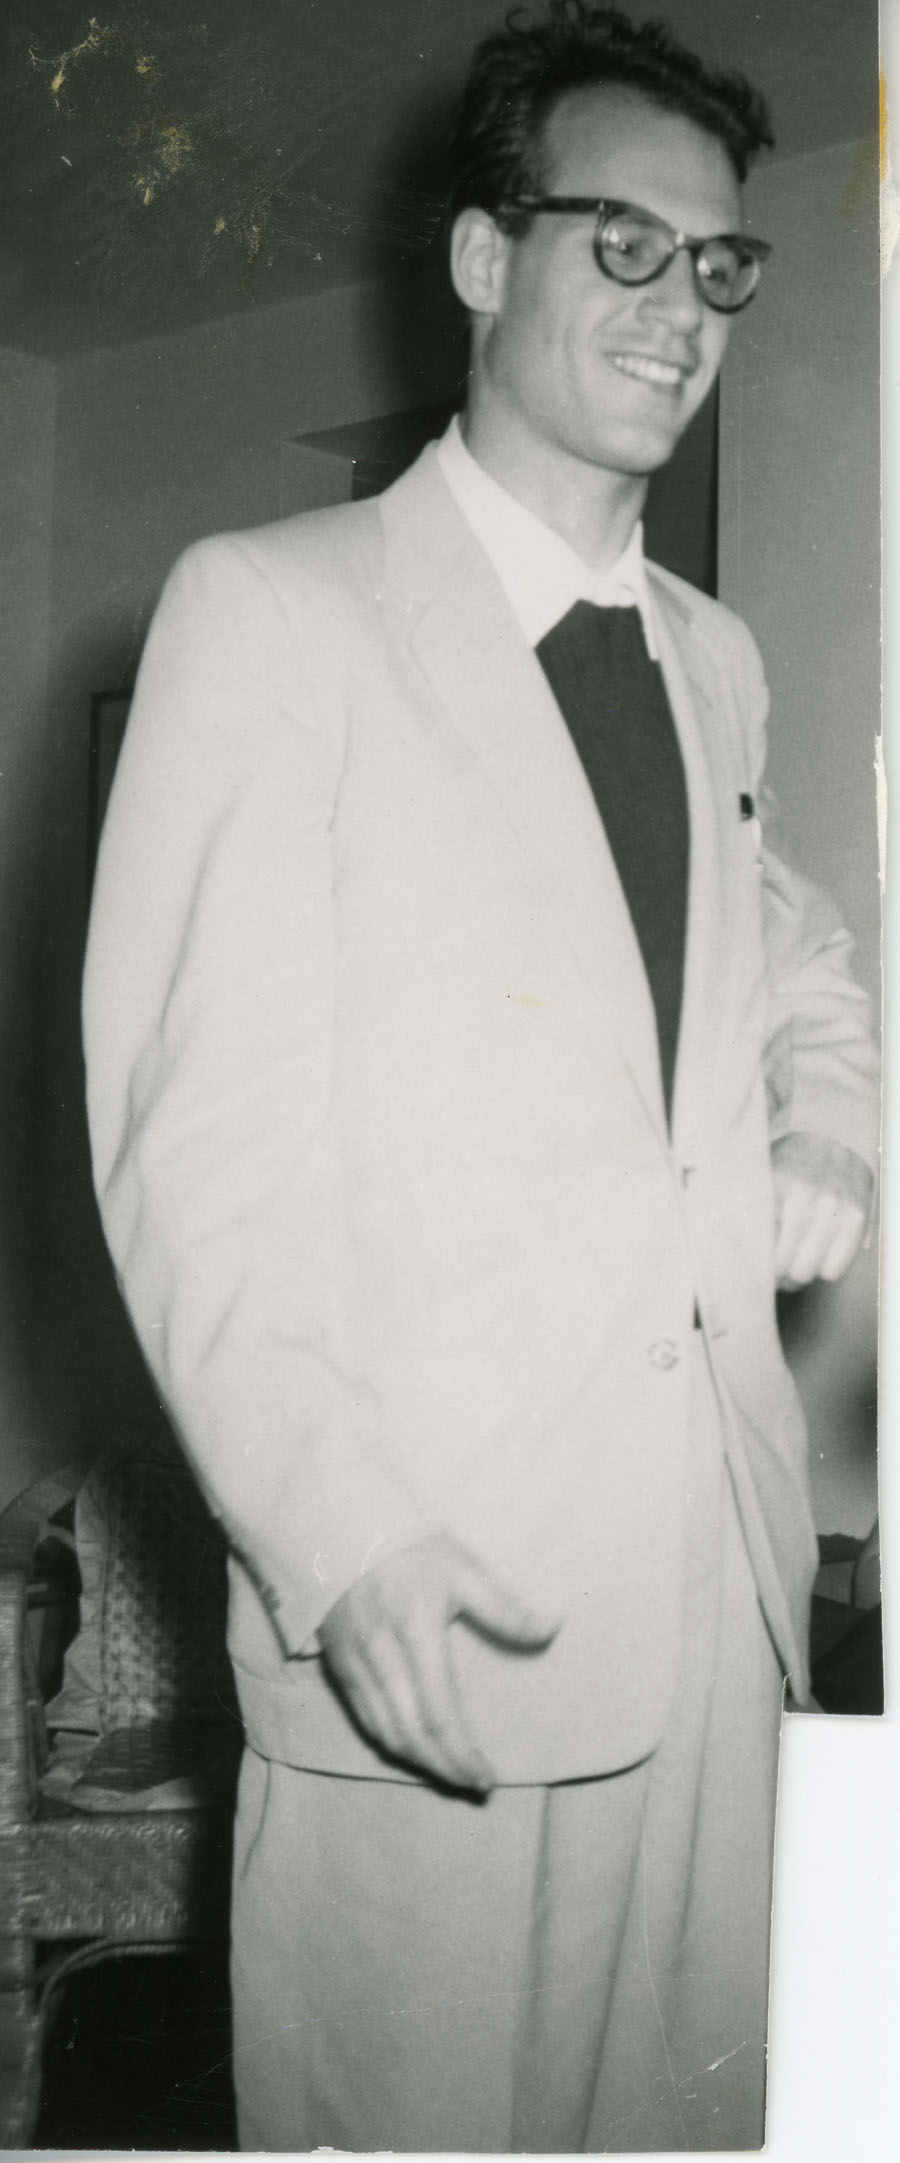
\includegraphics[scale = 1]{images/grothendieck}
		\caption{Alexander Grothendieck.}
	\end{center}
\end{figure}
% Paul R. Halmos photograph collection. 
% https://www.maa.org/press/periodicals/convergence/whos-that-mathematician-images-from-the-paul-r-halmos-photograph-collection-index#G

\begin{figure}
	\begin{center}
		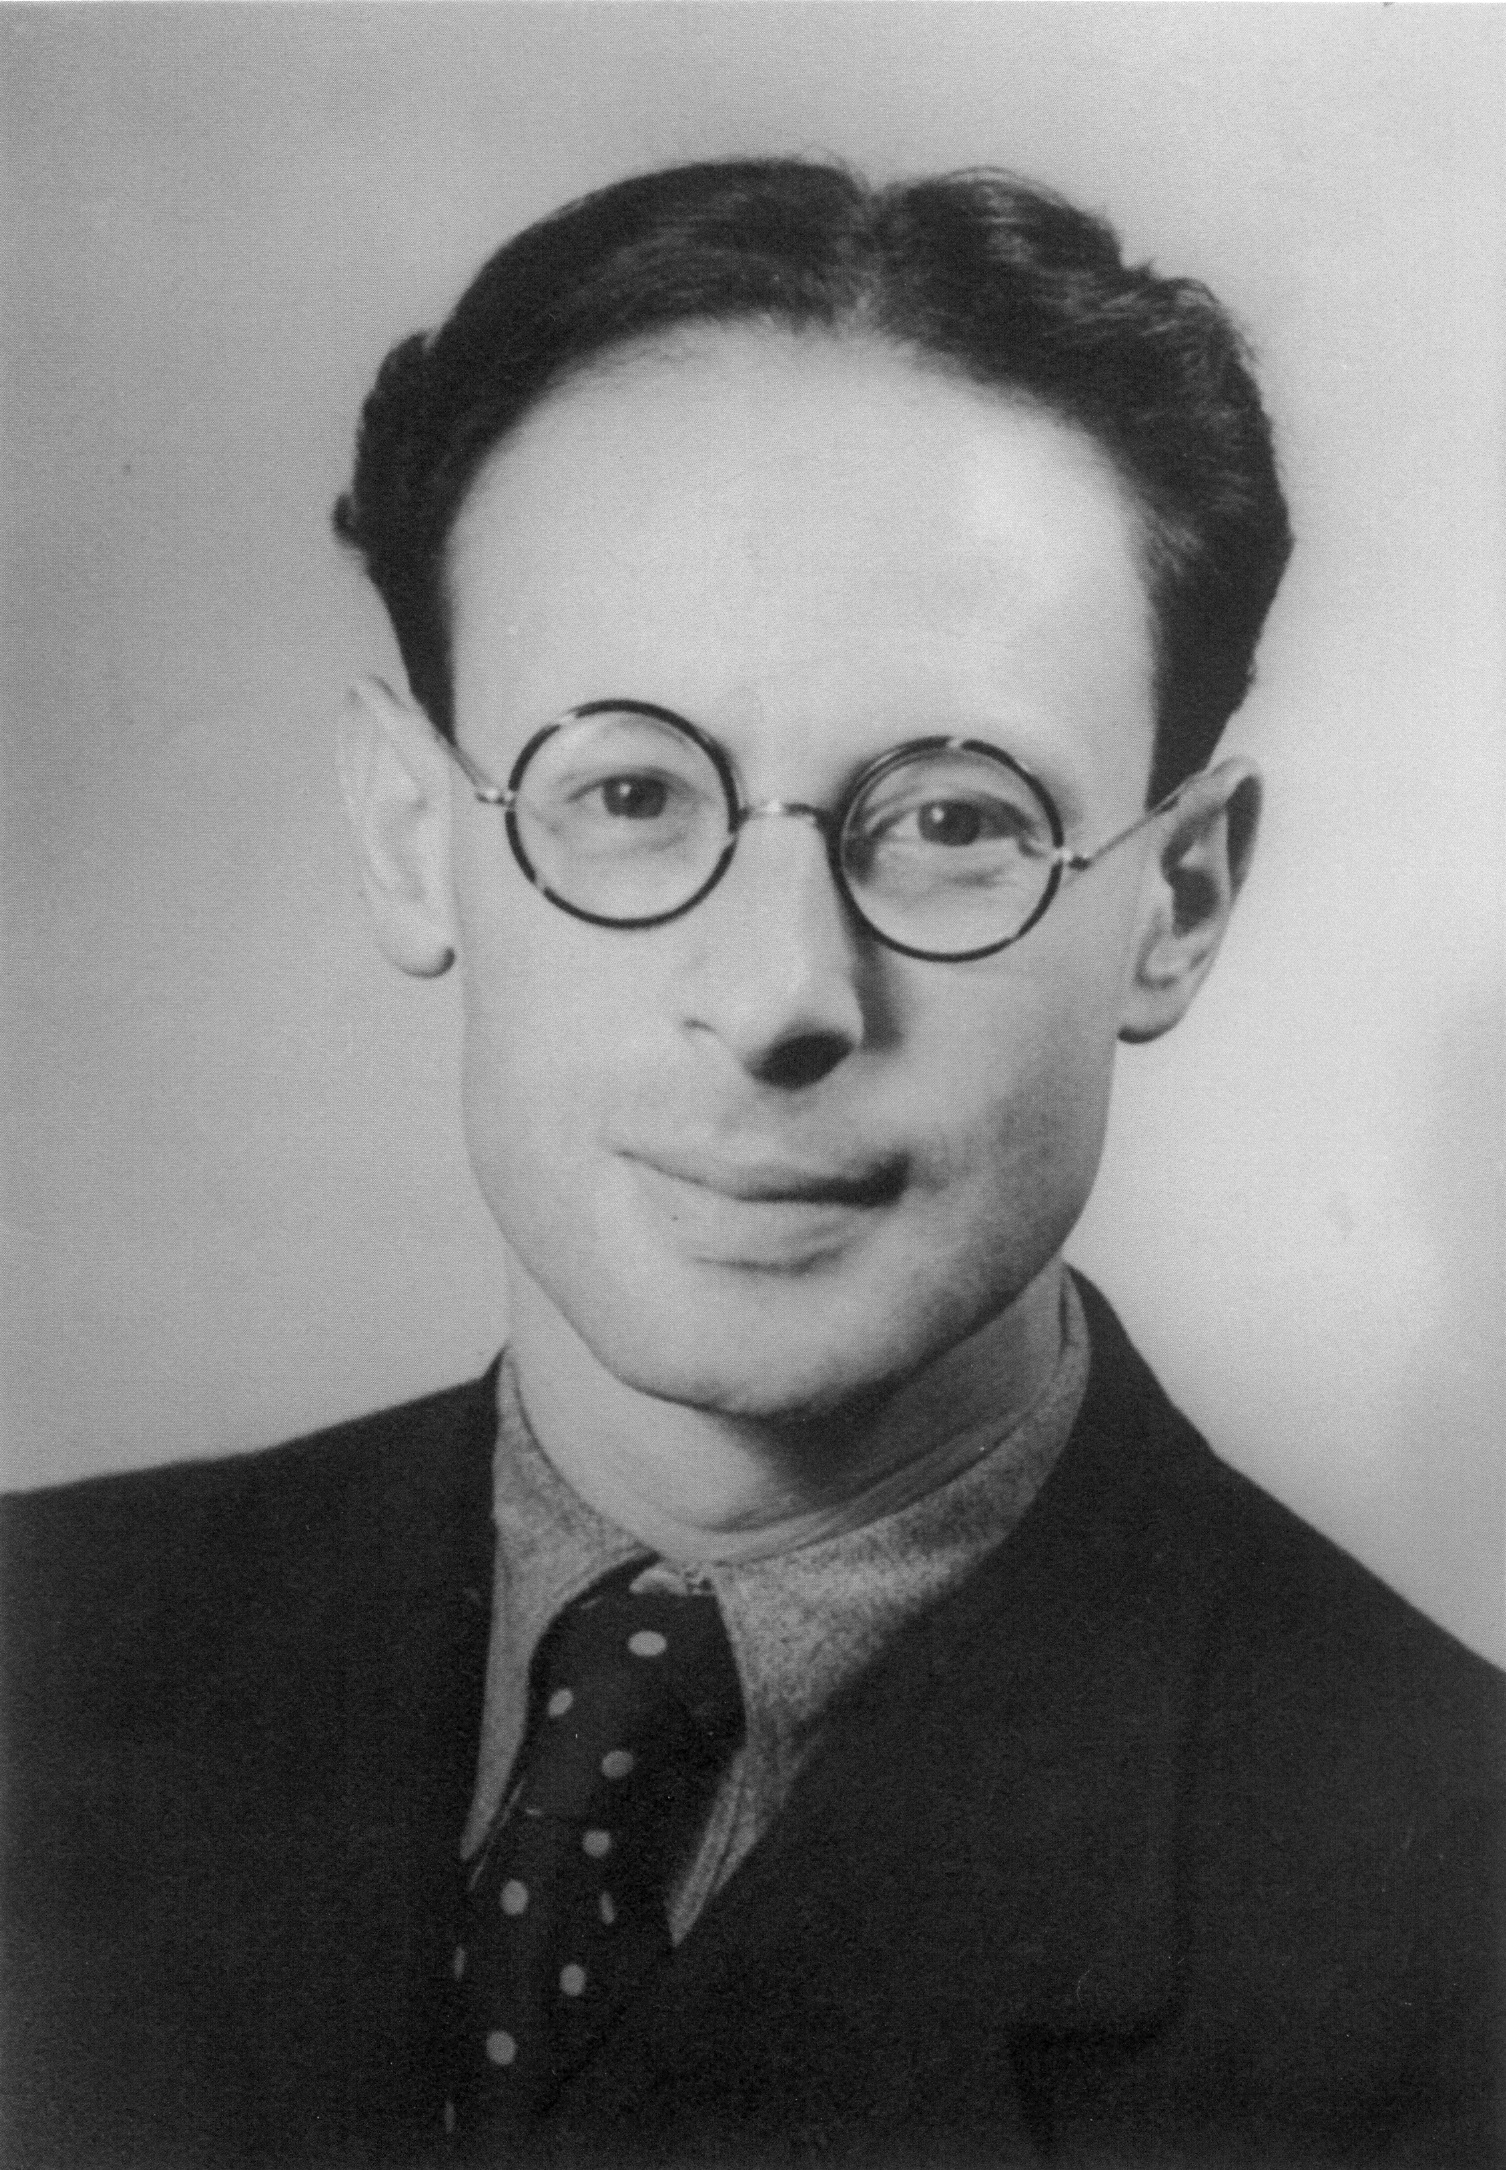
\includegraphics[scale = 0.4]{images/weil}
		\caption{Andr\'e Weil.}
	\end{center}
	\begin{center}
		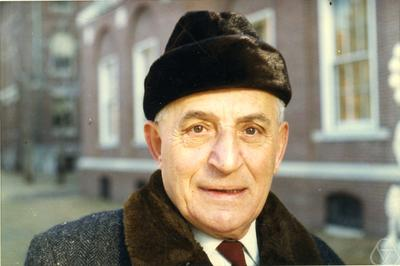
\includegraphics[scale = 0.75]{images/zariski}
		\caption{Oscar Zariski.}
	\end{center}
\end{figure}
% Sylvie Weil.
% https://attentionsw.org/about-andre-weil/

% Oberwolfach photo collection.
% https://opc.mfo.de/detail?photo_id=6262

\begin{figure}
	\begin{center}
		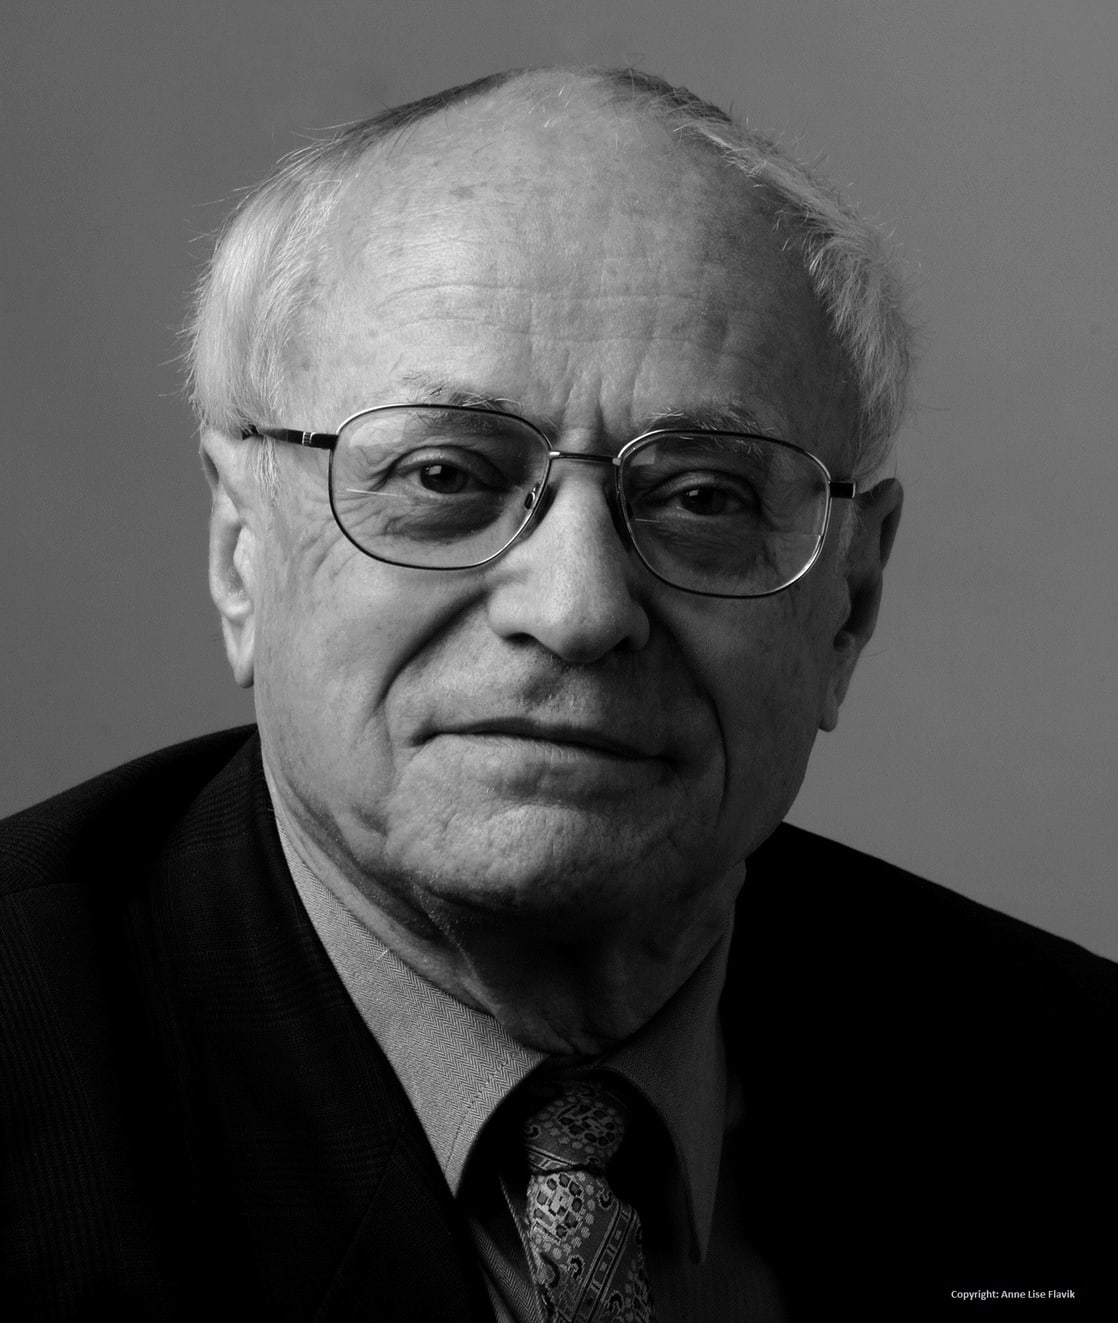
\includegraphics[scale = 0.19]{images/serre}
		\caption{Jean-Pierre Serre.}
	\end{center}
	\begin{center}
		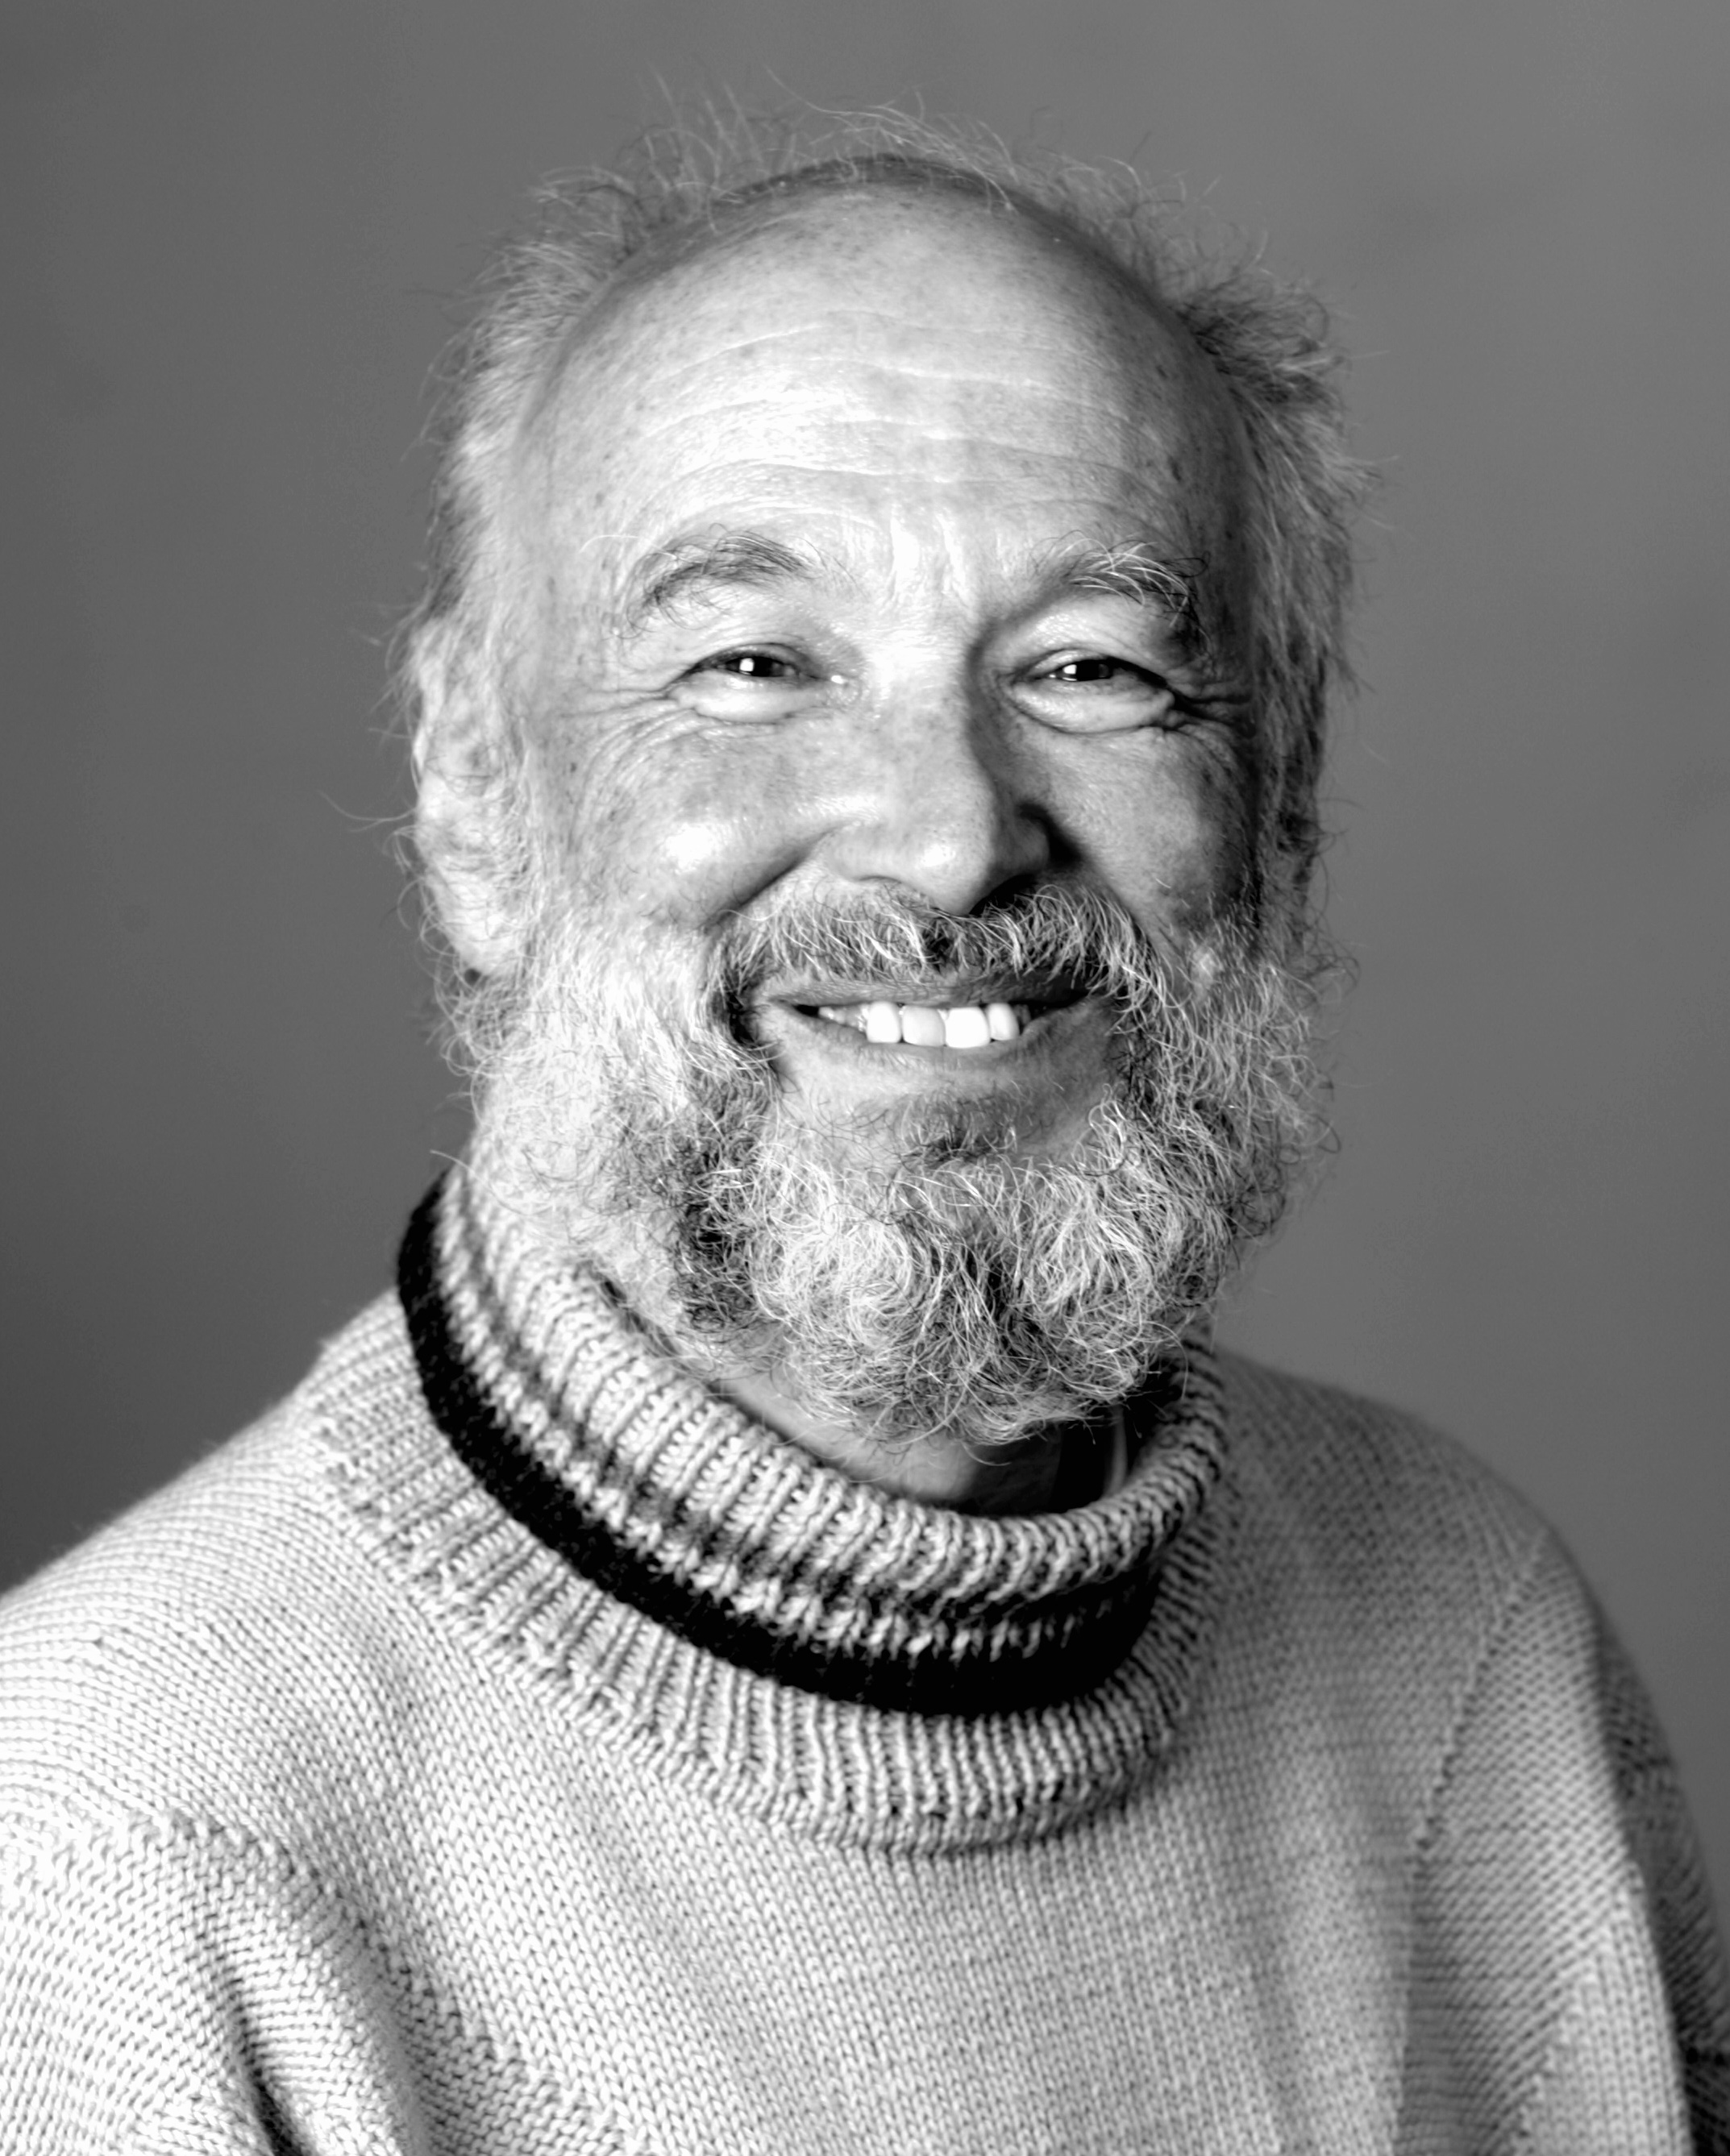
\includegraphics[scale = 0.1]{images/deligne}
		\caption{Pierre Deligne.}
	\end{center}
\end{figure}
% Abelprisen.
% https://abelprisen.no/page/images-media

\newpage

\tableofcontents
\ifams
	\vspace*{\fill}
\fi
\hypersetup{linkcolor = Red}
\newpage

\section{Varieties}
\subsection{Introduction.}
\begin{problem}
	Classify all Pythagorean triples.
\end{problem}
We would like to solve
\begin{align*}
	x^2 + y^2 = z^2
\end{align*}
where $x$, $y$, and $z$ are integers. We shall assume that $x$, $y$, and $z$ are coprime. We know that $x^2$, $y^2$, and $z^2$ are $0$ or $1$ mod $4$, and, analyzing the equation, we see that $z$ must be odd and $x$ and $y$ must have opposite parities. Without loss of generality, we shall let $y$ be odd, and, therefore, $x$ even.

We can rearrange this as follows:
\begin{align*}
	y^2 = (z-x) (z+x).
\end{align*}
Notice that $z-x$ is prime to $z+x$. Therefore, we can write $r^2 := z-x$ and $s^2 := z+x$, so
\begin{align*}
	z &= \frac{r^2+s^2}{2};\\
	x &= \frac{s^2-r^2}{2};\\
	y&=rs.
\end{align*}
Here, $r$ and $s$ are odd and coprime.

Let us look at this problem from a geometric perspective. Again, we would like to solve
\begin{align*}
	x^2+y^2=z^2
\end{align*}
in the integers. Write $X:= x/z$ and $Y := y/z$, so
\begin{align*}
	X^2 + Y^2 =1.
\end{align*}
Now, we would like to find rational points on the unit circle. Pick a rational point $(X,Y)$ on the unit circle and draw a line between it and $(-1,0)$. Call the point at which this line intersects the $y$-axis $(0,t)$.

One sees that
\begin{align*}
	t = \frac{Y}{X+1}.
\end{align*}
Therefore, since $Y = t(X+1)$ and $X^2 + Y^2 = 1$,
\begin{align*}
	(X+1) ((t^2+1) X + t^2-1) =0.
\end{align*}
One finds that the nontrivial solution to this quadratic gives
\begin{align*}
	X &= \frac{1-t^2}{1+t^2};\\
	Y &=\frac{2t}{1+t^2}.
\end{align*}
This gives a correspondence between the points on the unit circle that are not $(-1,0)$ and points on the $y$-axis. This is called a birational equivalence\index{birational equivalence}---roughly, an equivalence except on subsets of codimension at least $1$. 

This also gives rise to the infamous Weierstrass substitution: Write $\cos \theta := X$, so $\sin \theta = Y$ and $t= \tan \theta/2$. Then, if one has an integral in $\sin \theta$ and $\cos \theta$, one can let $t = \tan\theta/2$ and use these rational expressions for $\cos\theta$ and $\sin \theta$.

Try $t=1/2$. Then $X=3/5$ and $Y=4/5$, so we find that $3^2 + 4^2 = 5^2$.

From the geometric perspective, we see that the circle forms a group (that one can identify with the group of rotations). Suppose $(x_1,y_1)$ and $(x_2,y_2)$ are points on the circle. Then, if the group operation is $\cdot$, one finds that
\begin{align*}
	(x_1,y_1) \cdot (x_2,y_2) = (x_1x_2-y_1y_2, x_1y_2+x_2y_1).
\end{align*}
Of course, this comes from the once well-known identities
\begin{align*}
	\cos(\alpha+\beta) &=\cos\alpha \cos\beta- \sin \alpha \sin \beta;\\
	\sin(\alpha + \beta) &= \sin\alpha \cos\beta + \cos \alpha \sin \beta.
\end{align*}
This is one of the simplest examples of an algebraic group\index{algebraic group}. One can think of this as a functor
\begin{align*}
	G : \catn{Ring} \longrightarrow \catn{Grp}.
\end{align*}
That is, we can take a commutative ring $R$ to the set of pairs $(x,y)\in \R^2$ such that $x^2+y^2=1$. We define the group operation as above; the identity is given by the point $(1,0)$ and $(x,y) ^{-1} = (x,-y)$.

Notice that $G(\R)$ is the unit circle. What about $G(\C)$? Well, notice that $x^2+y^2 =1$ factorizes into
\begin{align*}
	(x+iy) (x-iy) = 1.
\end{align*}
Note that $x$ and $y$ are complex. Set $z := x+iy$, and we get the pair $(z,z^{-1})$. That is, this group is the set of all nonzero complex numbers.

There are many ways to view a circle:
\begin{enumerate}
	\item A subset of $\R^2$;
	\item A polynomial $z_2^2 + z_2^2 -1$;\footnote{These first two things define an algebraic set.}
	\item The ideal $(z_1^2+z_2^2-1)\subset \R[z_1,z_2]$;
	\item The ring $\R[z_1,z_2] / (z_1^2+z_2^2-1)$ (this is the coordinate ring\index{coordinate ring} of $S^1$);
	\item A (smooth) manifold;
	\item An algebraic group;
	\item A functor $\catn{Ring}\longrightarrow \catn{Grp}$ or $\catn{Ring} \longrightarrow \catn{Set}$.
\end{enumerate}

\subsection{Two cubic curves.}
Consider the curve
\begin{align*}
	y^2 = x^3 + x^2.
\end{align*}
Suppose $(x,y)$ is a rational point on this curve. Draw a line between this point and $(0,0)$. The slope of this line is $y/x=t$. If we choose a line through $(0,0)$ with rational slope, it will meet the cubic curve at one other rational point. That is, $(x,y)$ being rational corresponds to $t$ being rational. This is almost a one-to-one correspondence: $(0,0)$ corresponds to $t = \pm 1$. Using the equation of the cubic, one gets that $x=t^2-1$ and $y=t^3-t$. This is another birational equivalence.

One can think of this cubic curve as a copy of the rational line except that two of the points on the rational line are identified and mapped to the same point. This is a \index{resolution of a singularity}resolution of a singularity. This resolution is done by \index{blow up}blowing up. Hironaka proved that blowing up resolves singularities in characteristic zero.\footnote{``Resolution of singularities of an algebraic variety over a field of characteristic zero. I,'' 1964.}

\begin{example}[ ]
Find all rational points on 
\begin{align*}
	x^n+y^n = 1.
\end{align*}
Writing $x=X/Z$ and $y=Y/Z$ gives
\begin{align*}
	X^n + Y^n = Z^n.
\end{align*}
This is Fermat's last theorem, so finding rational points on curves can be hard.
\end{example}

\begin{example}[ ]\label{}\text{}
There are two glass spheres: One of radius $1$ and the other of radius $2$. Find two other glass spheres of rational radius that sum to the same value.\footnote{From problem 20 of \ul{The Canterbury Puzzles}.} That is, one wants to solve
\begin{align*}
	x^3 + y^3 = 1^3 + 2^3 = 9
\end{align*}
in $\Q$. The puzzle maker Henry Dudeney realized that
\begin{align*}
	x &= \frac{415280564497}{348671682660};\\
	y&= \frac{676702467503}{348671682660};
\end{align*}
formed another solution. 
\begin{quote}
	\small How does one get this, though?
\end{quote}

First, one draws the curve. We have two rational points on the curve already: $(1,2)$ and $(2,1)$. The tangent to $(1,2)$, for example, intersects the curve at a rational point: $(-17/7, 20/7)$. We require the coordinates be positive, though. So we draw a line between this point and $(2,1)$. The third intersection with the curve will also have rational coordinates. We determine that it is $(-271/ 438, 919/438)$. We continue this process and eventually get Dudeney's solution. 
\end{example}

This curve is not birational to a line. If a curve is birational to a line, it must be a complex sphere if one ignores some points. The curve $x^3 + y^3 =9$ looks like a torus with one point removed. Therefore, this example is fundamentally harder than the first curve and the circle.

We have an algebraic operation on this curve: Given two rational points $\alpha$ and $\beta$, we get another rational point $\alpha\cdot \beta$ by taking the third intersection of the curve and the line between $\alpha$ and $\beta$. If $\alpha$ and $\beta$ are the same point, we take the tangent to that point. Sometimes, though, we find that the line doesn't intersect with a third point. Defining a point at infinity solves this.

This operation defines a group. We let the identity be the point at infinity. We define the group law by $\alpha+\beta+\gamma = 0$ if and only if $\alpha$, $\beta$, and $\gamma$ lie on the same line.\footnote{The ``negative operation'' is what forms a group.} The operation is clearly commutative. What about associativity? It is very difficult to show that associativity holds with coordinates. However, it turns out that
\begin{align*}
	\alpha_1+\alpha_2+\cdots = \beta_1+\beta_2+\cdots
\end{align*}
if and only if there is a rational function $f$ with poles at the $\alpha_i$ and roots at the $\beta_i$. One can normally define a group structure like this on a curve.

Elliptic curves are the one-dimensional case of abelian varieties: Algebraic, projective groups.

\begin{definition}
Let $V$ be an $F$--vector space. A \defn{symplectic bilinear form} is a function $\omega : V\times V \longrightarrow F$ that satisfies the following conditions:
\begin{enumerate}
	\item $\omega$ is bilinear;
	\item $\omega(v,v)=0$ for all $v\in V$;
	\item If $\omega(w,v)$ for all $v\in V$, then $w=0$.
\end{enumerate}
\iffalse
The pair $(V,\omega)$ comprises a \defn{symplectic vector space}\index{symplectic vector space}.
\fi
\end{definition}

\begin{definition}
The \defn{symplectic group}\index{symplectic group} $\Sp(2n)$ is the group of $2n\times 2n$ matrices that preserve a symplectic bilinear form.
\end{definition}

\begin{warn}
	``Abelian linear group'' is an old name for ``symplectic group.'' Abelian linear groups are not necessarily abelian.
\end{warn}


\subsection{B\'ezout's theorem. Pappus's theorem. Pascal's theorem.}
\label{s_3}

\begin{theorem}[B\'ezout]
\label{}\index{B\'ezout's theorem}
Two curves of degrees $m$ and $n$ have at most $mn$ points of intersection unless they have a common component. Two curves of degrees $m$ and $n$ in the plane have $mn$ points of intersection over $\C$ counting points at infinity and multiplicities.\footnote{Newton proved something similar in \ul{Principia}, Sect. VI, Lemma XXVI.}
\end{theorem}

Suppose the curves are given by $f(x,y)=0$ and $g(x,y)=0$ of degrees $m$ and $n$ respectively. One can assume that the number of intersection points does not change if we perturb $f$ and $g$. Write $f=p_1\cdots p_m$ and $g = q_1\cdots q_n$ as products of linear factors. Then $f$ and $g$ are a union of $m$ and $n$ lines respectively, and the result follows.

There are problems with this argument, though: How do we know that perturbing $f$ and $g$ doesn't change the number of points of intersection, for example? Proofs like this were very common in algebraic geometry before Zariski and Weil.

We shall prove this theorem later.

\begin{theorem}[Pappus]\label{}\index{Pappus's theorem}
Take two lines in the plane. Choose three collinear points and label them $1$, $2$, and $3$. Choose three more collinear points and label them $1$, $2$, and $3$. From the first line to the second, connect $1$ with $2$ and $2$ with $1$, $1$ with $3$ and $3$ with $1$, and $2$ with $3$ and $3$ with $2$. The three points of intersection are collinear.
\end{theorem}

\begin{remark}
	Pappus's theorem is equivalent to commutativity. That is, a division ring is a field if and only if Pappus's theorem holds.
\end{remark}

\begin{theorem}[Pascal]\label{}\index{Pascal's theorem}
Take an ellipse and choose six points on it. Label two points $1$, two points $2$, and two points $3$. Connect them as in the statement of Pappus's theorem. The three points of intersection are collinear. 
\end{theorem}

\begin{remark}
	Pappus's theorem is a sort of degenerate case of Pascal's theorem.
\end{remark}

\begin{proof}
Label the lines $1$ through $6$ in the order described in the statement. Choose $6$ linear polynomials $p_1,\hdots, p_{6}$ such that $p_j = 0$ on line $j$. Consider the polynomials $p_1p_3p_5$ and $p_2p_4p_6$. These vanish at all six points. The polynomial $p_1p_3p_5 - \lambda p_2p_4p_6$ also vanishes at all $6$ points. Choose $\lambda$ such that $p_1p_3p_5 - \lambda p_2p_4p_6$ vanishes at a seventh point of the conic. This polynomial has degree $3$ and the conic has degree $2$. Therefore, by B\'ezout's theorem, there are at most $2\cdot 3 = 6<7$ intersection points unless the conic and the polynomial have a common component. The conic does not split into smaller-degree polynomials, so the only way the conic and the polynomial can have a common component is if the conic is contained in the polynomial. Thus, the degree-$3$ curve is the union of a conic and a line, and this line is Pascal's line since $p_1p_3p_5$ and $p_2p_4p_6$ vanish at the points of intersection and the points are normally not on the conic. 
\end{proof}

\subsection{Kakeya sets.}
A \defn{Kakeya set}\index{Kakeya set} is a set of points that contains a unit line in every direction. Examples include the radius-$1/2$ circle and the height-$1$ equilateral triangle. Kakeya conjectured that the smallest-area Kakeya set was the three-pointed deltoid.

\begin{figure}
	\begin{center}
		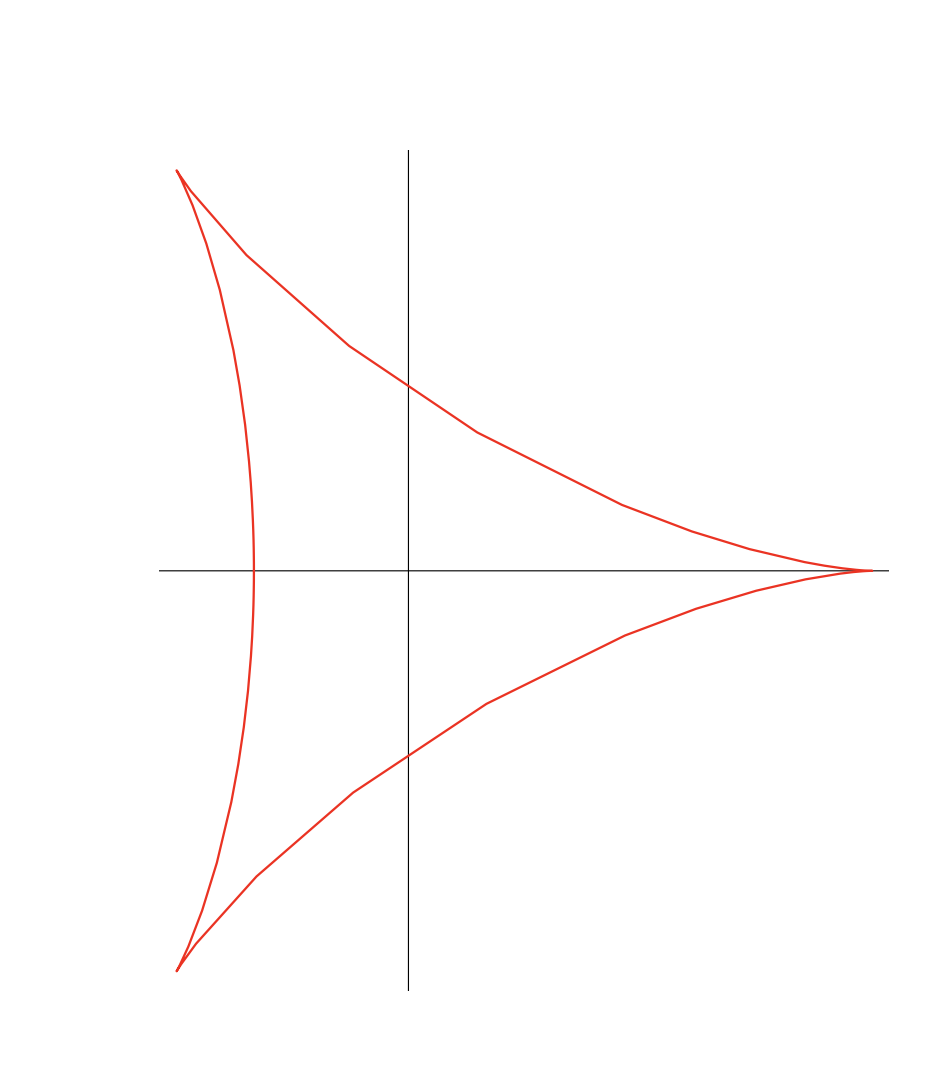
\includegraphics[scale=0.4]{images/kakeya_deltoid}
		\caption{The three-pointed deltoid.}
	\end{center}
\end{figure}

However, Besicovitch proved that there is no nonzero lower bound for the area of a Kakeya set. Thomas Wolff made the following conjecture that was proved by Dvir in 2008.\footnote{See \url{https://arxiv.org/abs/0803.2336}.}
\begin{theorem}[Wolff, Dvir]\label{}\index{}
The size of a Kakeya set over a finite field $F$ is bounded below by $c_n\left\lvert F \right\rvert ^n$.
\end{theorem}
Dvir proved this with $c_n = (n!)\inv$. The first step was to show that a Kakeya set cannot lie in a hypersurface of small degree. The second step was to show that, if a set is small, one can find a hypersurface of small degree containing it.

First, we claim that a Kakeya set in $F^n$ cannot lie in a hypersurface of degree $d<\left\lvert F \right\rvert $. Suppose $f$ is a polynomial of degree $d<\left\lvert F \right\rvert $ defining a hypersurface. Let $f_d$ be the highest-degree component. For all $v$, there exists $z$ such that $f(z+vt)$ vanishes for all $t$. That is, the roots of $f$ form a Kakeya set. Therefore, the coefficient $f_d(v)$ of $t^d$ vanishes. This is true for all $v$, and $f_d$ has degree less than $\left\lvert F \right\rvert $, so $f_d=0$. Thus, $f=0$.

Write 
\[
	\mathscr{C}(n,k) := \binom{n}{k}.
\]
The polynomials of degree less than or equal to $\left\lvert F \right\rvert -1$ form a vector space of dimension $\mathscr{C} ({n+\left\lvert F \right\rvert -1},{n})$. Therefore, one can find a hypersurface of degree at most $\left\lvert F \right\rvert -1$ vanishing on any set with less than $\mathscr{C}({n+\left\lvert F \right\rvert -1},{n})$ points.

Thus, one concludes that Kakeya sets have at least $\mathscr{C}({n+\left\lvert F \right\rvert -1},{n})$ points. This quantity is 
\begin{align*}
	\mathscr{C}({n+\left\lvert F \right\rvert -1},{n}) &=\binom{n+\left\lvert F \right\rvert -1}{n}\\
	&= \frac{(\left\lvert F \right\rvert ) \cdots (\left\lvert F \right\rvert +n-1)}{n!} \\
	&\ge \frac{\left\lvert F \right\rvert ^n}{n!}
\end{align*}
as required.

The following example is sometimes said to be the beginning of higher-dimensional algebraic geometry.

\begin{example}[$27$ lines on a cubic surface]\label{}
Cayley and Salmon proved that any nonsingular cubic surface has exactly $27$ lines on it. Consider the surface
\begin{align*}
	w^3 + x^3 +y^3 + z^3 = 0 \subset \mathbf{P}^3.
\end{align*}
Projective space $\mathbf{P}^3$ is the set of quadruples $(w,x,y,z)$ modulo the equivalence relation $(w,x,y,z)\sim  (\lambda w, \lambda x, \lambda y,\lambda z)$ for $\lambda\ne 0$. That is, if $z\ne 0$, one can take $\{(w,x,y,1)\} \isomto  \mathbf{C}^3$. One can see that $\mathbf{P}^3$ is covered by four copies of affine space. 

The line $(a,-a,b,-b)$ is on this surface. We can permute the coordinates and multiply by a cube root of unity. This gives $3^3 = 27$ lines.  
\end{example}

\subsection{Affine space. The Zariski topology.}
Let $K$ be a field. Then \index{affine space}affine space is almost the vector space $K^n$. The automorphisms of this vector space are all invertible linear transformations, given by $\GL_{n}(K)$. The automorphisms of affine space which one denotes $\mathbf{A}^n_K$ include $\GL_{n}(K)$ and translations $z \longmapsto z+v$. Therefore, the group of automorphisms of affine space is of dimension $n(n+1)$ and consists of matrices of the form
\begin{align*}
	\mat{*&*&*\\ \text{}*&*&*\\0&0&1}
\end{align*}
where the $2\times 2$ matrix in the top left has nonzero determinant. Roughly speaking, a vector space has an origin and an affine space does not. That is, one has a forgetful functor from vector spaces to affine spaces that forgets about the origin. One goes the other way by choosing an arbitrary origin. 

\iffalse Consider the three-dimensional pre-Einstein space in which we live. This is affine space blakdnkjdn Wait it has a metric\fi

\index{affine geometry}Affine geometry can be thought of as the study of the properties of affine space invariant under affine symmetries: invariant under translations and linear transformations. \iffalse Let us list some well-defined things in affine geometry:
\begin{itemize}
	\item Points;
	\item Lines;
	\item Parallel lines;
	\item Conics;
	\item Polynomial functions.
\end{itemize}
The following things are not well-defined.
\begin{itemize}
	\item Circles;
	\item Angles;
	\item Lengths.
\end{itemize}\fi Points, lines, parallel lines, conics, and polynomial functions are well defined in affine geometry. One realizes that circles, angle, and lengths, for example, are not well defined.

Algebraic geometry tends to use the \index{coordinate ring}coordinate ring of $\mathbf{A}^n_K$; that is, polynomials on the affine space: $K[z_1,\hdots, z_n]$. Given a coordinate ring, one can get an affine space $\mathbf{A}^n_K$ by taking the set of all $K$-algebra homomorphisms from the polynomial ring to $K$. The automorphism groups of these two things are the same, for example.

\begin{definition}[Algebraic set]\label{}
An \defn{algebraic set}\index{algebraic set} in $\mathbf{A}^n_K$ is the set of common roots of a set of polynomials in $K[z_1,\hdots, z_n]$.
\end{definition}

\begin{example}[ ]\label{}
The algebraic set of $\{x^2+y^2-1\}$ is a circle. That of $\{x-\alpha,y-\beta\}$ is $\{(\alpha,\beta)\}$.
\end{example}

Algebraic sets are closed under intersections. If $C_1,C_2,\hdots $ are the set of roots of $P_1,P_2,\hdots$ respectively, then $C_1\cap C_2\cap \cdots $ is the set of roots of $P_1\cup P_2\cup \cdots$. They are also closed under finite unions. If $C_1$ and $C_2$ are the sets of roots of $\{f_1,f_2,\hdots\}$ and $\{g_1,g_2,\hdots\}$, then $C_1\cup C_2$ is the set of roots of $\{f_ig_j\}$.

If a collection of sets is closed under intersections and finite unions, they form the closed sets of a topology. Therefore, \index{algebraic set}algebraic sets are the closed sets of the Zariski topology.\footnote{The intersections do not need to be of countably many sets.}

What are the closed sets of the affine line $\mathbf{A}^1_K$? The line is the set of roots of $0$. Any finite set consists of the roots of a polynomial $(z-\alpha_1)(z-\alpha_2)\cdots(z-\alpha_n)$. One can check that $\mathbf{A}^1_K$ and finite sets are the only closed sets. One notes that this topology is not Hausdorff.

What about $\mathbf{A}^2_K$? We have sets of points $\{(\alpha,\beta)\}$ that is the set of common roots of $\{x-\alpha, y-\beta\}$. We also have any algebraic curve $f(x,y) =0$. Therefore, a typical closed set in $\mathbf{A}^2_K$ consists of finitely many algebraic curves and points. One notices that the Zariski topology on $\mathbf{A}^2_K$ is not the product topology on $\mathbf{A}^1_K\times \mathbf{A}^1_K$. The latter is a finite number of vertical lines, horizontal lines, and points.

\begin{example}[Determinantal variety]\label{}
One can think of $\mathbf{A}^{mn}_K$ as the vector space $\Hom_K(K^m,K^n)$ of dimension $mn$. One example of an algebraic set is the set of all linear transformations of rank at most $r$, which gives a \index{determinantal variety}determinantal variety. For example, the subset of surjections $K^m\longrightarrow K^n$ is open in the Zariski topology.
\end{example}

\subsection{Noetherian spaces.}
\begin{definition}[ ]\label{}
A \defn{Noetherian ring}\index{Noetherian ring} $R$ satisfies one of these three equivalent conditions:
\begin{enumerate}
	\item Every ideal of $R$ is finitely generated;
	\item Every nonempty set of ideals has a maximal element;
	\item Every increasing chain of ideals stabilizes. 
\end{enumerate}
\end{definition}

\begin{example}[ ]\label{}
The ring $K[z_1,\hdots,z_n]$ is Noetherian. Hilbert originally proved this. Noether gave a much simpler proof as follows. She showed that if $R$ is Noetherian, then $R[z]$ is Noetherian. Consider $R$-ideals $I_0\subseteq I_1\subseteq\cdots$ where $I_n$ is given by the leading coefficients of polynomials of degree less than or equal to $n$ in an $R$-ideal $I$. We know that $I_N=I_{N+1}=\cdots$ for some $N$ since $R$ is Noetherian. Take finite sets of polynomials $S_0,\hdots, S_N$ where $S_k$ contains polynomials of degree $k$ whose leading coefficients generate $I_k$. One can check that $S_0,\hdots, S_N$ generate $I$. 
\end{example}

\begin{definition}[ ]\label{}
A topological space is a \defn{Noetherian topological space}\index{Noetherian topological space} if, equivalently,
\begin{enumerate}
	\item The closed sets satisfy the descending chain condition, so any decreasing chain of closed sets stabilizes;
	\item Any nonempty collection of closed sets has a minimal element.
\end{enumerate}
\end{definition}
 \begin{remark}
 	The affine space $\mathbf{A}^n_K$ with the Zariski topology is Noetherian. Closed sets of $\mathbf{A}^n_K$ correspond to some ideals of the coordinate ring $K[z_1,\hdots, z_n]$.\footnote{Any closed set is determined by the ideal of functions vanishing on it.}
 \end{remark}

Noetherian spaces are weird. The Noetherian condition is equivalent to saying that every open set is (quasi)compact.\footnote{Bourbaki changed the definition of ``compact'' to ``compact and Hausdorff,'' but it turned out that there were non-Hausdorff compact sets, so they used the term ``quasicompact.''\index{compact}\index{quasicompact} {See \ul{General Topology}, \S 9.I, p. 83.}}

\begin{exercise}\label{}
Show that, if a topological space is Noetherian and Hausdorff, then it is finite.
\end{exercise}

\begin{definition}[ ]\label{}
A topological space is called an \defn{irreducible topological space}\index{irreducible topological space} if it is nonempty and not the union of two proper closed subsets.
\end{definition}

Recall that a typical closed set of $\mathbf{A}^2_K$ is a finite number of curves and points. The curves are irreducible. An affine line, for example, is irreducible since any two nonempty closed sets intersect. This space seems to be the union of a finite number of irreducible subsets.

\begin{theorem}[ ]\label{}\index{}
Any Noetherian space is a finite union of irreducible subspaces.
\end{theorem}

\begin{proof}
This follows from Noetherian induction. Every closed subset is a finite union of irreducibles. If not, pick a minimal counterexample $C$. If $C$ is irreducible, then we are done, since we have a contradiction. If $C$ is not irreducible, then we can write $C=C_1\cup C_2$ where $C_1$ and $C_2$ are smaller closed subsets. By induction, $C_1$ and $C_2$ are finite unions of irreducibles and, therefore, $C$ is. This is a contradiction. 
\end{proof}

\begin{corollary}[ ]\label{}
Every algebraic set is a finite union of irreducible algebraic sets.
\end{corollary}

\begin{remark}
	Irreducible algebraic sets are sort of (provisionally) \index{algebraic variety}algebraic varieties.
\end{remark}

\begin{example}[ ]\label{}
Consider the variety $xy=1$ and the set of nonzero points in $\mathbf{A}^1$. The temporary definition of an algebraic variety means that the set of nonzero points is not an algebraic variety. However, one sees that these two objects are isomorphic. We shall address this later.
\end{example}

\begin{example}[ ]\label{}
Consider the algebraic set $\{x^2+y^2 -2z^2=0, 2x^2 - y^2 - z^2=0\}$. This turns out to be a union of four irreducible subsets (lines): $x=y=z$, $x=-y=z$, $x=-y=-z$, and $x=y=-z$. The intersection of irreducible subsets does not need to be irreducible.
\end{example}

\begin{example}[ ]\label{}
Take $xy=0$. This is reducible but connected. Now, consider $xy=1$. This is irreducible, and it certainly doesn't look connected. However, it is connected in the Zariski topology (of course, it isn't in the Euclidean topology).
\end{example}


\subsection{The weak Nullstellensatz.}
Let us study the relationship between subsets of an affine space $\mathbf{A}^n$ and ideals of $K[z_1,\hdots, z_n]$. One can map a subset $Y$ to the ideal $\II(Y)$ given by polynomials vanishing on $Y$. Conversely, an ideal $\mathfrak{a}$ can be mapped to a subset $\ZZ(\mathfrak a)$ given by the set of roots of $\mathfrak{a}$. What is the relationship between these two maps? Well, $\ZZ(\II(Y))$ is the closure of $Y$ in the Zariski topology. Further, $\II(\ZZ(\mathfrak{a}))\ne \mathfrak{a}$. For example, take $\mathfrak{a}=(z^2)\subset K[z]$. Then, $\ZZ(\mathfrak{a}) = \{0\}$, so $\II(\ZZ(\mathfrak{a})) =(z)\ne (z^2)$. More generally, if $f^n\in \mathfrak{a}$, then $f\in \II(\ZZ(\mathfrak a))$. So, $\sqrt{\mathfrak{a}} \subseteq \II(\ZZ(\mathfrak{a}))$. Recall that the radical of an ideal\index{radical of an ideal} ${\mathfrak a}$ is
\begin{align*}
	\sqrt{\mathfrak{a}} = \mathfrak{r}(\mathfrak{a}) := \{ r\in R : r^n \in \mathfrak{a} \textrm{ for some $n$}\}.
\end{align*}
This is an ideal.

\begin{problem}
	Does $\sqrt{\mathfrak{a}}= \II(\ZZ(\mathfrak{a})) $ hold?
\end{problem}

No: Take $\mathfrak{a} = (z^2 + 1) \subset \R[z]$. Notice that $\ZZ(\mathfrak{a})= \emptyset$, so $\II(\ZZ(\mathfrak{a})) = \mathbf{R}[z]\ne \mathfrak{a}$.\footnote{The field $\mathbf{R}$ is not algebraically closed.} However, if $\Omega$ is algebraically closed, then equality holds.\footnote{This is Hilbert's \index{Nullstellensatz}Nullstellensatz.}

\begin{problem}
	What are the maximal ideals of $K[z_1,\hdots, z_n]$?
\end{problem}

There are some obvious ones. Take $(a_1,\hdots, a_n)\in \mathbf{A}^n$. Consider the ideal $(z_1-a_1,\hdots, z_n-a_n)$. This consists of the functions vanishing on $(a_1,\hdots, a_n)$. It is maximal because its quotient by the ring is $K$. Are these all maximal ideals? No, but that's true if $K$ is algebraically closed. This is \cref{wen}. Let us prove this.

First, we shall show that if $K$ is a field and finitely generated as an algebra over $L$, then $K$ is a finitely generated module over $L$. We're going to cheat by assuming that $L$ is uncountable. Notice that $K$ is of at most countable dimension as a module since it is finitely generated as an algebra. If $z\in K$ is transcendental over $L$, then the elements $1/(z-a)$ for $a\in L$ form an uncountable, linearly independent set. This is a contradiction. Therefore, all elements $z\in K$ are algebraic over $L$. Since $K$ is finitely generated as an algebra, $K$ is finitely generated as a module (or vector space).\footnote{One does not require $L$ to be uncountable: The finite number of generators of $K$ only have poles on a finite number of irreducible subsets of the affine space over $L$, but there are an infinite number of such irreducible subsets.}

Suppose $I$ is a maximal ideal of $L[z_1,\hdots, z_n]$. We want to show that $I = (z_1-a_1,\hdots, z_n-a_n)$ for some $(a_1,\hdots, a_n)$. Put $K = L[z_1,\hdots, z_n]/I$, which is a field since $I$ is maximal. The field $K$ is also finitely generated by an algebra (generated by $z_1,\hdots, z_n$). By  the previous ``lemma,'' $K$ is finitely generated as a module; that is, $K$ is algebraic over $L$. However, $L$ is algebraically closed, so $L=K$. Therefore, $z_i\in K$, so $z_i=a_i$ for some $a_i\in L$. This implies that $I\supseteq (z_1-a_1,\hdots, z_n-a_n)$. So $I = (z_1-a_1,\hdots, z_n-a_n)$. The weak Nullstellensatz follows.


\subsection{The strong Nullstellensatz.}
Suppose that $K$ is an algebraically closed field.

\begin{theorem}[Weak Nullstellensatz]\label{wen}\index{}
The maximal ideals of $K[z_1,\hdots, z_n]$ correspond to points in affine space.
\end{theorem}

\begin{theorem}[Strong Nullstellensatz]\label{stn}\index{}
Suppose that $\mathfrak{a}\subseteq K[z_1,\hdots, z_n]$ is an ideal. Then, 
\begin{align*}
	\II(\ZZ(\mathfrak{a})) = \sqrt{\mathfrak{a}} .
\end{align*}
\end{theorem}

\begin{proof}
It is straightforward to show that $\sqrt{\mathfrak{a}} \subseteq \II(\ZZ(\mathfrak{a}))$. We shall employ the Rabinowitsch trick.\footnote{See ``Zum Hilbertschen Nullstellensatz,'' 1929.} Suppose $\mathfrak{a}$ is generated by $f_1,\hdots, f_m$ and $f\in \II(\ZZ(\mathfrak{a}))$. We want to show $f\in \II(\ZZ(\mathfrak{a}))$. This means that $f$ vanishes if $f_1,\hdots, f_m$ vanish. Therefore, $f_1,\hdots, f_m$ and $1-z_0f$ have no common roots in $\mathbf{A}^{n+1}$.\footnote{Bringing in another variable is the trick of Rabinowitsch.} Apply \cref{wen} to $\mathbf{A}^{n+1}$. Therefore, $f_1,\hdots, f_m, 1-x_0f$ generate the unit ideal, so $1 = g_0(1-z_0f)+g_1f_1 +\cdots + g_mf_m$ for some $g_i$. Put $z_0=1/f$, so $1=g_1f_1+\cdots +g_mf_m$ where $g_i \in K[z_1,\hdots, z_n, 1/f]$. Clearing denominators, one has
\begin{align*}
	f^N = h_1f_1+\cdots + h_mf_m
\end{align*}
where $h_i=g_if^N\in K[z_1,\hdots, z_n]$. That is, $f\in \sqrt{(f_1,\hdots, f_m)} $.
\end{proof}

Hilbert's Nullstellensatz gives a correspondence between affine space $\mathbf{A}^n$ and the ring $K[z_1,\hdots, z_n]$. Points correspond to maximal ideals. Algebraic sets correspond to radical ideals $\mathfrak{a} = \sqrt{\mathfrak{a}} $. More generally, closed subschemes correspond to ideals.

\begin{example}[ ]\label{}
Consider the line $y=0$ that corresponds to the ideal $(y)$ and the parabola $y=x^2$ that corresponds to the ideal $(y-x^2)$. These are radical ideals. One takes the intersection of these two varieties by taking $(y-x^2, y)$. This ideal is not radical, since $\sqrt{(y, x^2)}=(x,y)$ as an ideal which corresponds to $(0,0)$ as a point in affine space.
\end{example}


\begin{example}[Nilpotent matrices]\label{}
Recall that $A\in \MM_n(K)$ is nilpotent if and only if $A^n = 0$. One can think of $\MM_n(K)$ as $\mathbf{A}^{n^2}$. If $A = (a_{ij})$, then $A^n$ is something complicated, but one can suppose that its entries generate the ideal $I$ in the coordinate ring of $\mathbf{A}^{n^2}$. 
\begin{quote}
	\small Does $I=\sqrt{I}$ hold?
\end{quote} 
No: If $A$ is nilpotent, then all of its eigenvalues are $0$, so its trace is $0$. However, $\sum_{j}^{} a_{jj}\notin I$, since $I$ is generated by homogeneous polynomials of degree $n$ and $\sum_{j}^{} a_{jj} \in \sqrt{I} $ by \cref{stn}.

Take $n=2$. If 
\begin{align*}
	A = \mat{a&b\\c&d}
\end{align*}
is nilpotent, then
\begin{align*}
	A^2 = \mat{a^2 + bc&b(a+d)\\c (a+d) &d^2 + bc} = 0.
\end{align*}
Hence $I=   (a^2+bc,\, b(a+d), \,c (a+d),\,d^2 + bc)$. Some power of $a+d$ is an element of $I$. Exercise: Show that $(a+d)^2\notin I$ but $(a+d)^3\in I$.
\end{example}

\begin{example}[Commuting matrices]\label{}
Write $A=(a_{ij})$ and $B=(b_{ij})$. Then $AB-BA$ is something; let its entries generate the ideal $I$ in the coordinate ring of $\mathbf{A}^{2n^2}$. Whether or not $I=\sqrt{I}$ holds is an open problem. The question of whether an ideal $I\subset R$ is radical is the same as asking whether $R/I$ has nilpotent elements.\footnote{The space of pairs of commuting matrices is a notoriously difficult space to study.}
\end{example}

\subsection{The Lasker--Noether theorem.}
Algebraic sets correspond to radical ideals of $K[z_1,\hdots, z_n]$. Also, an algebraic set is a finite union of irreducible algebraic sets. Irreducible algebraic sets correspond to prime ideals.\footnote{An $R$-ideal $\mathfrak{p}$ is prime if and only if $R/\mathfrak{p}$ is an integral domain.}

\begin{theorem}[ ]\label{}\index{}
A radical ideal is a finite intersection of prime ideals.
\end{theorem}

This is a translation of the previously-mentioned result into ring-theoretic language.
\begin{theorem}[Lasker]\label{}\index{}
An ideal of $K[z_1,\hdots, z_n]$ is a finite intersection of primary ideals.
\end{theorem}
\begin{theorem}[Noether]\label{}\index{}
This holds for ideals of Noetherian rings.
\end{theorem}\index{Lasker--Noether theorem}
\iffalse
\begin{remark}
	Emmanuel Lasker was World Chess Champion for 27 years, which is the longest anyone has held this title. He proved the theorem above during his reign.
\end{remark}
\fi

\begin{definition}\label{}
An $R$-ideal $\mathfrak{p}$ is \defn{primary}\index{primary ideal} if and only if $ab\in \mathfrak{p}$ implies $a\in \mathfrak{p}$ or $b^n\in \mathfrak{p}$ for some $n$.
\end{definition}

Alternatively, suppose if $ab=0$ where $a\in R$ and $b\in R/\mathfrak{p}$ then $b=0$ or $a^n=0$ for some $n$. Then $R/\mathfrak{p}$ is \defn{coprimary}\index{coprimary module}. The module $R/\mathfrak{p}$ is coprimary if and only if $\mathfrak{p}$ is primary.

\begin{definition}[ ]\label{}
A module $M$ is coprimary if and only if it has at most one associated prime.
\end{definition}

\begin{definition}[ ]\label{}
An \defn{associated prime}\index{associated prime} $\mathfrak{p}$ of a $R$-module $M$ is a prime ideal such that $M$ contains a submodule isomorphic to $R/\mathfrak{p}$.
\end{definition}
\begin{remark}
If $R$ is Noetherian, these two definitions of coprimary are equivalent for finitely generated modules.
\end{remark}

If one has modules $M\supseteq N$, $N$ is primary if and only if $M/N$ is coprimary.

\begin{theorem}[Lasker--Noether]\label{}\index{}
Let $M$ be a finitely generated module over a Noetherian ring $R$. The ideal $(0)$ is an intersection of primary submodules of $M$. Equivalently, $M$ is contained in a finite direct sum of coprimary modules.
\end{theorem}

For $\mathbf{Z}$-modules, coprimary modules include $\mathbf{Z}^n$ where $\mathfrak{p}=(0)$ and any finite group of order $p^f$ where $\mathfrak{p} = (p)$. Recall that abelian groups are a direct sum of free abelian groups and groups of prime power order.

\subsection{The proof of the Lasker--Noether theorem.}
The video in which Dr. Borcherds proves the Lasker--Noether theorem is incomprehensible, so this section comes from a video from his series on commutative algebra.\footnote{The link: \url{https://www.youtube.com/watch?v=GLmXzrusM2M}.}

Let $M$ be a finitely generated module over a Noetherian ring $R$. Recall that $M$ is coprimary if it has at most one associated prime. We shall prove that
\begin{align*}
	M \subseteq \bigoplus_{\mathfrak{p}\in \Ass M} M_{\mathfrak{p}}
\end{align*}
where each $M_{\mathfrak{p}}$ is coprimary with associated prime $ \mathfrak{p}$. 

There is no such thing as a primary module. The original version of the theorem says that if $I\subseteq R$ is an ideal, then $I$ is a finite intersection of primary ideals. Lasker originally proved this for polynomial rings over fields $K$ or $\mathbf{Z}$. His proof was incredibly long. Noether generalized the result to all Noetherian rings. Her proof was notably simpler.

The second version is as follows. Suppose we have modules $N\subseteq M$. Then, $N$ is a finite intersection of primary submodules.

\begin{definition}[ ]\label{}
A submodule $X$ is called a \defn{primary submodule}\index{primary submodule} of $M$ if $rm\in X$ implies $m\in X$ or $r^nM\subseteq X$ for some $n>0$.
\end{definition}

Notice that, if $M=R$, then a submodule is an ideal, and this becomes Lasker's definition of a primary ideal. One notes that this is not a property of $X$; it is a property of how $X$ is embedded in $M$. In particular, it is a property of the quotient $Y:= M/X$. If $r$ is a zero divisor of $Y$, then $r^nY=0$ for some $n>0$. The module $Y$ with this property is coprimary. We will show that this definition and the one mentioned earlier are equivalent for finitely generated modules.

The third version of the Lasker--Noether theorem says that
\begin{align*}
	M \subseteq \prod_{\mathfrak{p}\in \Ass M} M_{\mathfrak{p}}
\end{align*}
where $M_{\mathfrak{p}}$ is coprimary. In fact, the second version implies this one. 

Take $N=0$, so $0 = \bigcap J_{\mathfrak{p} }$ where $J_{\mathfrak{p}}$ is a primary submodule. That is, the natural map $M \longrightarrow \prod M/J_{\mathfrak{p}}$ is injective.\footnote{The kernel is the intersection, which is $0$.} Although $J_{\mathfrak{p}}$ is a primary submodule, the quotient is coprimary.

We have two definitions for ``coprimary'':
\begin{enumerate}
	\item There is at most one associated prime;
	\item $rm = 0$ implies $m=0$ or $r^nM=0$ for some $n>0$.
\end{enumerate}

Suppose that $n\ne 0$ and $m\in M$. Put $\mathfrak{p} = \Ann(m)$. Then the second definition implies $\mathfrak{p} \subseteq \sqrt{\Ann (M)} $. If $\mathfrak{p}$ is prime, then $\Ann(M)\subseteq \Ann (m)= \mathfrak{p}$, so $\sqrt{\Ann(M)}\subseteq \mathfrak{p} $. That is, if $\mathfrak{p}\in \Ass M$, $\mathfrak{p} = \sqrt{\Ann (M)} $. Thus, there is at most $1$ associated prime given by the radical of the annihilator of $M$. So (2) implies (1).

Assume $\Ann M=0$. Put $\Ass M = \{\mathfrak{p}\}$. This associated prime contains $\Ann (m)$ given $m\ne 0$. Therefore, we need to show that $\mathfrak{p}$ is nilpotent. Suppose that $a\in \mathfrak{p}$ is nilpotent. Then, the localization $M[a^{-1}]$ is nonzero. If $z\in M$ is $0$ in $M[a^{-1}]$ , then $za^n=0$ for some $n$. That is, $M[a^{-1}]=0$ implies $a^n \in \Ann M$ for some $n$, since some power kills any element of $M$ and $M$ is finitely generated. But $\Ann M=0$ by assumption, so $a$ is nilpotent. 

Since $M[a^{-1}]\ne 0$, one has $\Ass (M[a^{-1}])\ne \emptyset$ (primes of $R[a^{-1}]$). Pick $T\in \Ass (M[a^{-1}])$, an ideal of $R[a^{-1}]$. Let $\mathfrak{q}$ be the preimage of $T$ in $R$.\footnote{Recall that one has $R\longrightarrow  R[a^{-1}]$, $\mathfrak{q}\longrightarrow T$, $\mathfrak{q}\subseteq R$, and $T\subseteq R[a^{-1}]$.} Both $T$ and $\mathfrak{q}$ are primes, and $\mathfrak{q}$ is the union of $\Ann(m)\subseteq \Ann (ma)\subseteq \Ann (ma^2)\subseteq \cdots$.\footnote{One verifies that $\mathfrak{q}$ is everything that annihilates $ma^n$.} This is an increasing sequence in a Noetherian ring, so it stabilizes. Therefore, $\mathfrak{q}=\Ann(ma^n)$ for some $n$. Hence, $\mathfrak{q}\in \Ass(M)$ since it is prime and the annihilator of some element in $M$. But $a\in \mathfrak{p}$ and $a\notin \mathfrak{q}$ because $a$ is a unit of $M[a^{-1}]$ and if $a\in \mathfrak{q}$ then $M[a^{-1}]=0$. So, $\mathfrak{p}\ne \mathfrak{q}$, so $M$ has at least $2$ associated primes. Contradiction. So (1) implies (2).

Now, we prove the Lasker--Noether theorem: That is, 
\begin{align*}
	M\subseteq \prod_{\mathfrak{p} \in \Ass M} M_{\mathfrak{p}}
\end{align*}
where $M_{\mathfrak{p}}$ is coprimary.  

If it is not true, pick a maximal submodule $N$ such that $M/N$ is not contained in a product of coprimary ideals. We may assume that $N=0$ by modding out by $N$. Notice that $M$ is not coprimary, so it has $2$ submodules $M_1\isomto R/\mathfrak{p}_1$ and $M_2\isomto R/\mathfrak{p}_2$ where $\mathfrak{p}_1\ne \mathfrak{p}_2$ are prime ideals. Then, for $z\in R/\mathfrak{p}_1- \{0\}$, $\Ann(z)= \mathfrak{p}_1$, and similarly for $\mathfrak{p}_2$. Therefore, $M_1\cap M_2=0$. Consider this exact sequence:
\begin{align*}
	M_1\cap M_2 \longrightarrow M\longrightarrow M/M_1 \oplus M/M_2.
\end{align*}
Since the intersection is zero, the second arrow is injective. Moreover, we assumed that $0$ is the maximal submodule not a product of coprimary modules, so each quotient is contained in a product of coprimary modules. Therefore, $M$ is contained in a product of coprimary modules. The Lasker--Noether theorem follows.

Take $M=R/I$. We have 
\begin{align*}
	R/I = M \subseteq \prod_{} R/I_{\mathfrak{p}}.
\end{align*}
We know that the $R/I_{\mathfrak{p}}$, so $I_{\mathfrak{p}}$ must be primary in Lasker's sense. Therefore, $I=\bigcap I_{\mathfrak{p}}$.

\subsection{Quotients of varieties by groups.}
Recall that any algebraic set $Y$ has a coordinate ring $K[z_1,\hdots, z_n]/\II(Y)$. This coordinate ring is a $K$-algebra, is finitely generated, and has no nilpotent elements. Further, a ring with these three properties corresponds to an algebraic set by the Nullstellensatz.\footnote{This algebraic set is not unique: It depends on one's choice of generators. The corresponding algebraic sets are isomorphic in some sense.} One can think of algebraic sets up to some kind of isomorphism as being equivalent to rings with these three properties. The category of algebraic sets is equivalent to the opposite category of coordinate rings. 

Suppose $Y$ is an algebraic set acted on by a group $G$. Can we form a quotient $Y/G$? One cannot form a quotient by identifying points of $Y$ with elements of $G$. One views this problem from the perspective of coordinate rings. 

If the group $G$ acts on the algebraic set $Y$, it will act on the corresponding coordinate ring. Therefore, we look at the ring of invariants $(K[z_1,\hdots,z_n]/\II(Y))^G$. If the invariant ring satisfies the three previous properties, then it is the coordinate ring of an algebraic set, so it is reasonable to call it $Y/G$.

This invariant ring is clearly a $K$-algebra. It has no nilpotent elements, either. But is it finitely generated? Hilbert proved that it is in many cases, but Nagata proved that that's not always the case.\footnote{``On the fourteenth problem of Hilbert,'' 1958, \url{https://web.archive.org/web/20131102202816/http://www.mathunion.org/ICM/ICM1958/Main/icm1958.0459.0462.ocr.pdf}.}

\begin{example}[ ]\label{}
Suppose $G=\Sg_n$ acts on $\mathbf{A}^n$ by permuting coordinates. Then, $K[z_1,\hdots, z_n]^G$ is the ring of invariant functions generated by the elementary invariant polynomials. Hence, one sees that $\mathbf{A}^n/\Sg_n\isomto \mathbf{A}^n$.\footnote{This works out so nicely because $\Sg_n$ is a reflection group.}
\end{example}


If $\Zmod 2$ acts on the real line by $z\longmapsto -z$, one might think that the quotient is a half-closed interval. This is what one gets by identifying points under the group, but, by the construction above, it's the real line. One identifies $2$ and $-2$, but also identifies $2i$ and $-2i$.\footnote{These are real points of the quotient.}


 \begin{example}[ ]\label{}
Suppose $\GL_{n}(K)$ acts on $K^n$. The orbits are either $0$ or everything else, so one believes that the quotient will have two points. However, it only has one, since the only invariant polynomials acted on by $\GL_{n}(K)$ are constants. That is, we get the field $K$: The coordinate ring of a point.
\end{example}

\begin{example}[Classical invariant theory]\label{}
The group $G=\SL_{2}(\mathbf{C})$ acts on binary quantics (binary forms) $a_nz^n + a_{n-1}z^{n-1}y + \cdots +a_0y^n$. One has $(a_0,\hdots, a_n)\in \mathbf{A}^{n+1}$. What is the quotient $\mathbf{A}^{n+1}/\SL_{2}(\mathbf{C})$? The coordinate ring of this will be all polynomials in $a_n,a_{n-1},\hdots$ invariant under $\SL_{2}(\mathbf{C})$. These are called \index{invariant}``invariants.''

Take $a_2z^2 + a_1zy + a_0y^2$. A typical invariant is the discriminant given by $a_1^2 - 4a_0a_2$. Paul Gordan proved that the ring of invariants was finitely generated.\footnote{See \ul{Mathematics of the 19th Century: Mathematical Logic, Algebra, Number Theory, Probability Theory}, 2001, p. 85.} Gordan was known as the ``king of invariant theory.'' His proof was convoluted, and Hilbert figured out a way to prove that rings of invariants were finitely generated. We shall look at this in the next section.
\end{example}

\subsection{Hilbert's finiteness theorem.}
Let $A = K[z_1,\hdots, z_n]$. Let $G$ be a group acting on $K^n$ spanned by $z_1,\hdots, z_n$. That is, the group $G$ acts on $A$. We consider $A^G$: The invariant elements of $A$ under the action of $G$.

\begin{theorem}[Hilbert]\label{}\index{Hilbert's finiteness theorem}
The invariant ring $A^G$ is finitely generated as a $K$-algebra if $G$ is finite and $\chr K = 0$.
\end{theorem}
\begin{remark}
	Hilbert proved this for almost any reductive group. The restriction on the characteristic of $K$ is not necessary, but it simplifies the proof.
\end{remark}

Notice that $A$ is graded by degree, so $A = A_0\oplus A_1\oplus A_2\oplus \cdots$. Let $I$ be the ideal of $A$ generated by the homogeneous elements of $A^G$ of degree greater than $0$. Notice that $I$ is finitely generated as an ideal. We can assume that $I$ has a finite number of generators in $A^G$; these generators are homogeneous. 

Suppose that $I=(i_1,\hdots,i_n)$ as above. We would like to show that these elements generate $A^G$ as a $K$-algebra. Suppose that $A=K[z_1,z_2]$ and $I = (z_2)$. Even though $I$ is finitely generated as an ideal, the ring it gives is not finitely generated as a ring or as an algebra.\footnote{It is generated by $z_2,z_1z_2, z_1^2z_2,\hdots$.} 

The ring of invariants $A^G$ of $A$ has a Reynolds operator\index{Reynolds operator} $\rho$. The Reynolds operator $\rho(a)$ of $a$ is the average of $a$ under $G$, so
\begin{align*}
	\rho(a) = \frac{1}{\left\lvert G \right\rvert } \sum_{g\in G}^{} g(a).
\end{align*}
Notice that we needed that $G$ is finite and $\chr K = 0$. It has the following properties:
\begin{itemize}
	\item $\rho(1)=1$;
	\item $\rho(a+b) = \rho (a)+\rho (b)$;
	\item $\rho(ab) = a\rho (b)=\rho(a)\rho (b)$ if $\rho(a)=a$.
\end{itemize}
Notice that $\rho$ is not a homomorphism of algebras. However, $\rho$ is an $A^G$-module homomorphism from $A$ to $A^G$.

We shall prove Hilbert's theorem by induction on the degree to show that, if $z\in A^G$ is homogeneous, then $z$ is in the algebra generated by $i_1,\hdots,i_n$. This is trivial for degree $0$. Suppose $\deg z > 0$. One has
\begin{align*}
	z=a_1i_1 + \cdots +a_ni_n
\end{align*}
for some homogeneous $a_i\in A$ since $z$ is in the ideal generated by $i_1,\hdots, i_n$. The $a_i$s need not be in $A^G$, though. One gets
\begin{align*}
	z &= \rho(z)\\ 
	  &= \rho(a_1)i_1 + \cdots +\rho(a_n)i_n
\end{align*}
since $z\in A^G$ and $\rho(i_j)=i_j$. Notice that $\rho(a_j) \in A^G$ by the properties of the Reynolds operator and $i_j\in A^G$ by assumption. So, $z$ is a polynomial in elements of $A^G$ of smaller degree; that is, $\deg \rho(a_j)<\deg z$. Therefore, by induction, $z$ is in the algebra generated by $i_1,\hdots, i_n$. Hilbert's finiteness theorem follows.

Suppose $G$ is compact and $K=\mathbf{R}$ or $K=\mathbf{C}$. The same proof works. One defines 
\begin{align*}
	\rho(a) = \frac{1}{\Vol (G)}\int_{G}^{} g(a) \, d\mu
\end{align*}		
with respect to the Haar measure on the group. Hilbert studied the case $G=\SL_{n}(\mathbf{C})$. Here, one can apply Weyl's unitarian trick: Notice that $\SL_{n}(\mathbf{C})\supset \SU_n(\mathbf{C})$ and $\SU_n(\mathbf{C})$ is compact. Complex actions of $\SL_{n}(\mathbf{C})$ on finite-dimensional complex vector spaces $V$ are ``the same'' as actions of $\SU_n(\mathbf{C})$ on $V$.\footnote{The complexification of the Lie algebra of $\SU_n(\mathbf{C})$ is the same as the Lie algebra of $\SL_{n}(\mathbf{C})$.}

Let's study Nagata's counterexample. The group
\begin{align*}
	K = \left\{ \mat{1&*\\0&1} \right\} 
\end{align*}
acts on $K^2$.\footnote{This comes up in counterexamples often. It is a unipotent action in which all eigenvalues are $1$.} Now, $K^{16}$ acts on $K^{32}$. Let $G$ be a ``generic'' $13$-dimensional subspace of $K^{16}$. 


\subsection{Three examples of quotients.}

\begin{example}[Cyclic quotient singularity]\label{}\index{cyclic quotient singularity}
Consider $\mathbf{A}^2$, whose coordinate ring is $K[y_1,y_2]$. Let $G=\Zmod n$. Suppose that $G$ is generated by $\sigma$ of order $6$. Let $\zeta$ be an $n$th root of unity. Then, $G$ acts on the coordinate ring by $\sigma y_1 = \zeta y_1$ and $\sigma y_2= \zeta y_2$. One determines the quotient of $\mathbf{A}^2$ by $G$ with the invariants of $K[y_1,y_2]$. Notice that 
\begin{align*}
	\sigma(y_1^iy_2^j) &= \zeta^{i+j} y_1^iy_2^j
\end{align*}
which is $y_1^iy_2^j$ if and only if $i+j\equiv 0\pmod n$. Therefore, the ring of invariants has a basis $y_1^iy_2^j$ satisfying the condition mentioned. If $n=3$, the ring of invariants is generated by $z_0:=y_1^3$, $z_1:=y_1^2y_2$, $z_2:=y_1y_2^2$, and $z_3:=y_2^3$. These are not independent: one notices that
\begin{align*}
	z_iz_j = z_kz_\ell
\end{align*}
if $i+j=k+\ell$. Hence, the ring of invariants is
\begin{align*}
	K[z_0,z_1,z_2,z_3] / (z_1z_2-z_0z_3, z_1^2 z_0z_2, z_2^2-z_1z_3). 
\end{align*}
\end{example}

\begin{example}[The parameter space of cyclohexane]\label{}\index{parameter space}
\iffalse In a parameter space, points correspond to ``configurations''---some algebraic subset of a variety, for example.\fi Points correspond to ``configurations'' in a parameter space. The centre of each carbon atom is specified by three numbers. Therefore, $\mathbf{A}^{18}$ is the parameter space for six carbon atoms. However, there are some conditions the atoms in cyclohexane must satisfy. Any two adjacent carbon atoms are at a fixed distance. If the first two carbon atoms are located at $(x_1,y_1,z_1)$ and $(x_2,y_2,z_2)$, then one requires $(x_1-x_2)^2 + (y_1-y_2)^2 + (z_1-z_2)^2=\lambda$ for some fixed $\lambda$. Thus, we have six quadrics for these distances. Furthermore, bond angles must be fixed. These angles can be specified by the distances between every other carbon atom, so we get six more quadrics. One is led to believe that the parameter space is of dimension $18-6-6$, but we have translations and rotations. Therefore, one ought to take the space of (lower bound) dimension $18-6-6$ and mod out by the group of translations and rotations. There are three degrees of freedom and the group of rotations is three-dimensional, so the group by which we quotient out is of dimension $6$. 

What is the dimension of this parameter space? The obvious guess is  
\[
	(18-6-6) - (3+3)=0,
\] 
but this is wrong: Hermann Sachse (1890) discovered two distinct conformations of cyclohexane: ``Chair'' and ``boat.'' The ``boat'' conformation is flexible, so to speak, and the ``chair'' conformation is rigid. Therefore, the parameter space has (at least) one point corresponding to the ``chair'' conformation and one $1$-dimensional component corresponding to the ``boat'' conformation. That is, the na\"ive guess for the dimension of the quotient was wrong.
\end{example}
\iffalse
\begin{figure}
	\begin{center}
		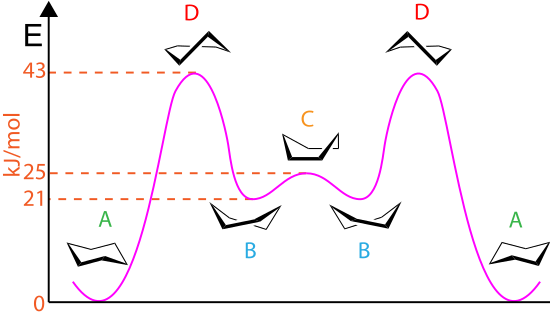
\includegraphics[scale=0.5]{images/cyclohexane_conformations}
		\caption{The conformations of cyclohexane.}
	\end{center}
\end{figure}
\fi
\begin{example}[Moduli space of elliptic curves]\label{}
A \index{moduli space}moduli space is a space whose points correspond to isomorphism classes of things.\footnote{It is tradition to use ``parameter space'' when the thing is embedded in something else and ``moduli space'' otherwise.} An \index{elliptic curve}elliptic curve over $\mathbf{C}$ is a nonsingular curve topologically isomorphic to a torus. Any elliptic curve in the form \[ y^2=x^3+ax^2+bx+c = (x-\alpha) (x-\beta) (x-\gamma).\] One can make some changes of variables to get the elliptic curve into the form
\begin{align*}
	y^2 = x(x-1) (x-\lambda)\quad\textrm{where}\quad \lambda \ne 0,1.
\end{align*}
Note that this does not change the isomorphism classes. One gets the impression that elliptic curves are classified by numbers $\lambda$, but this is invariant under $\lambda\longmapsto 1/\lambda$ and $\lambda \longmapsto 1-\lambda$. Therefore, it is also invariant under
\begin{align*}
	\lambda &\longmapsto \frac{1}{1-\lambda};\\
	\lambda&\longmapsto \frac{\lambda}{\lambda-1};\\
	\lambda&\longmapsto \frac{\lambda-1}{\lambda};
\end{align*}
etc. These six transformations form a group isomorphic to $\Sg_3$. We get this affine variety $\mathbf{A}^1 - \{0,1\}$ modulo $\Sg_3$. This is an affine variety: If $\lambda\in \mathbf{A}^1-\{0,1\}$, one can think of this set as the curve $\lambda(\lambda-1)\mu = 1\subset\mathbf{A}^2$. What is this space $(\mathbf{A}^1 - \{0,1\}) / \Sg_3$, exactly? Its coordinate ring is $K[\lambda, 1/\lambda, 1/(\lambda-1)]$, so one considers the ring of invariants under $\Sg_3$. The simplest invariant element is 
\begin{align*}
	j(\lambda) =  \frac{2^8(\lambda^2-\lambda+1)^3}{\lambda^2(\lambda-1)^2}.
\end{align*}
It turns out that $K[\lambda, 1/\lambda, 1/(\lambda-1)]^{\Sg_3} \isomto K[j]$. This is the so-called \index{$j$-invariant}\defn{$j$-invariant} of an elliptic curve.
\end{example}


\subsection{Dimension.}
Dimension\index{dimension} first was thought of as the number of parameters needed to define a point. However, this fails: Cantor showed that $\mathbf{R}^2$ and $\mathbf{R}$ have the same number of points. Peano and Hilbert showed that there are continuous maps from $\mathbf{R}$ onto $\mathbf{R}^2$. So, in a sense, one does not need two parameters to describe points in $\mathbf{R}^2$.\footnote{This makes sense if one looks at smooth manifolds.}

The second attempt was the \index{Lebesgue covering dimension}Lebesgue covering dimension: A set has dimension at most $n$ if every open cover has a refinement such that each point is in at most $n+1$ sets. This works for Euclidean space but isn't all that useful in algebraic geometry.

The next definition is due to Brouwer, Menger, and Urysohn: The boundary of a topological space should have smaller dimension than the topological space. A topological space has dimension at most $n$, then, if all points have arbitrarily small neighbourhoods whose boundary has dimension less than $n$. Traditionally, this definition is used for separable metric spaces, and the spaces one encounters in algebraic geometry are not separable or metrizable. However, this definition works well for definitions of algebraic sets.\footnote{This is called \index{inductive dimension}``inductive dimension,'' by the way.} If $\dim$ is the inductive dimension, one has
\begin{align*}
	\dim \emptyset := -1.
\end{align*}

Next, one has the \defn{Krull dimension}\index{Krull dimension}: The supremum of the numbers $n$ for which there is a chain
\begin{align*}
	Z_0\subsetneq Z_1\subsetneq \cdots \subsetneq Z_n
\end{align*}
of irreducible subsets. This only works well for Noetherian spaces. All Hausdorff spaces have Krull dimension $0$. Note that, in the case of Noetherian spaces, the Brouwer--Menger--Urysohn (inductive) dimension is the same as the Krull dimension.

\begin{remark}
	One uses the Krull dimension over the inductive dimension for historical reasons.
\end{remark}

One gets various variations on the \index{Hausdorff dimension}Hausdorff dimension, which is determined by counting the number of balls used to cover a metric space and then seeing what happens to the number of balls as the radii tend to $0$.\footnote{Interestingly, Hausdorff dimensions do not need to be integers; they don't need to be rational, either.} It isn't really relevant here, though.

One might consider transfinite dimensions\index{transfinite dimension}. Again, this isn't pertinent here.

Also, one can consider the \index{deviation of a poset}deviation of a poset. A poset has deviation at most an ordinal $\alpha$ if, for all descending chains, almost all intervals of the chain have deviation less than $\alpha$. For Noetherian rings, one looks at a poset of ideals; then, the deviation is the Krull dimension. This works well for modules and noncommutative rings. Notice that some posets do not have a deviation: for example, $\mathbf{Q}$. This means that there are some weird non-Noetherian commutative rings that do not have a deviation.\footnote{For non-Noetherian rings, there doesn't seem to be a good definition for ``dimension.''}

Now, we move on to algebraic definitions. The idea is that a set of high dimension has many functions on it.

Suppose that $B$ is a variety over a field $K$. Look at the field of fractions of the coordinate ring of $B$. Set the dimension of $B$ to be the transcendence degree of the field of fractions.\footnote{Recall that the transcendence degree is the largest number of algebraically indepdent elements in the field.} If $B=\mathbf{A}^2$, the coordinate ring is $K[z_1,z_2]$, so the field of fractions is rational functions in two variables. This, clearly, has transcendence degree $2$. This works for algebraic varieties, but it doesn't work for more general objects in algebraic geometry: For example, for non-irreducible algebraic sets.\footnote{Which don't have a fields of fractions.} This doesn't work well for schemes, either: $\Spec \Z$ should have dimension $1$, but this definition gives $0$.

Next, one has the \index{Hilbert polynomial}Hilbert polynomial. This works for local rings $A$.\footnote{Recall that a ring is a \index{local ring}local ring if and only if it has a unique maximal ideal $\mathfrak{m}$.} The (length of) dimension $\dim(A/\mathfrak{m}^k)$ is a polynomial in $k$ for large $k$ of degree $d$. Hence, one defines
\[
	\dim A := d.
\] 
Consider the local ring $K [\![z_1,\hdots, z_n]\!]$ which has the maximal ideal $\mathfrak{m} = (z_1,\hdots, z_n)$. The dimension of $A/\mathfrak{m}$ is $1$, that of $A/\mathfrak{m}^2$ is $1+n$, that of $A/\mathfrak{m}^3$ is $1+n+n(n+1)/2$, etc.

One also considers the Gelfand--Kirillov dimension\index{Gelfand--Kirillov dimension} of a ring, which applies to finitely-generated algebras over a field. It is given by
\begin{align*}
	\limsup_{n} \log \dim R_n / \log n
\end{align*}
where $R_n$ is the subspace generated by monomials in some set of generators of length at most $n$. This isn't of much concern to us, either, since we are concerned with commutative rings and the Hilbert polynomial suffices.

One can define the \index{dimension of the tangent space of a point}dimension of the tangent space of a point of a variety. This works for nonsingular varieties/schemes. For example, if one considers the point $(0,0)$ on the singular curve $y^2=x^3+x^2$, the tangent space will look two-dimensional though you want it to be one-dimensional. However, this is a useful concept because one can define the notion of a singular point with it: a space is nonsingular at a point if the dimension of the tangent space is equal to its dimension.

One can also look at the minimum number of elements in a system of parameters. This works, but it's not intuitive. 
\begin{quote}
	\small What's a system of parameters?
\end{quote}
A \index{system of parameters}\defn{system of parameters} for a local Noetherian ring of Krull dimension $d$ with maximal ideal $\mathfrak{m}$ is a set of elements $z_1,\hdots, z_d$ that satisfies these equivalent conditions:
\begin{enumerate}
	\item $\mathfrak{m}$ is a minimal prime over $(z_1,\hdots, z_d)$;
	\item The radical $\mathfrak{r}{(z_1,\hdots, z_d)}=\mathfrak{m} $;
	\item Some power of $\mathfrak{m}$ is contained in $(z_1,\hdots, z_d)$;
	\item $(z_1,\hdots, z_d)$ is $\mathfrak{m}$-primary.
\end{enumerate}

Finally, one has various notions of \index{homological dimension}homological dimension.

\subsection{Projective space.}
\begin{definition}[ ]\label{}
\defn{Projective space}\index{projective space} $\mathbf{P}^n_K$ is the set of all $1$-dimensional subspaces of $K^{n+1}$.
\end{definition}

We use coordinates as follows: $(z_0:z_1:\cdots : z_n)\sim (\lambda z_0:\lambda z_1:\cdots:\lambda x_n)$ where not all $z_i=0$ and $\lambda\in K - \{0\}$.

If $z_0\ne 0$, we can write
\begin{align*}
	(z_0:z_1:\cdots:z_n) = (1:y_1:\cdots : y_n)
\end{align*}
where $y_i = z_i/z_0$. Therefore, $\mathbf{P}^n \supset \mathbf{A}^n$. If $z_0=0$, we get a copy of $\mathbf{P}^{n-1}_K$. Therefore, $\mathbf{P}^n_K$ is a disjoint union $\mathbf{A}^n_K \sqcup \mathbf{P}^{n-1}_K $. One thinks of the points of $\mathbf{P}^{n-1}_K$ as ``\index{point at infinity}points at infinity.''

Consider $\mathbf{P}^n_{\mathbf{R}}$. One has $(z_0:\cdots:z_n)$, which one can rescale such that $z_0^2 +\cdots+z_n^2 = 1$. There are exactly two points, then, corresponding to the same line: $(z_0:\cdots:z_n)$ and $(-z_0:\cdots:-z_n)$. These correspond to antipodal points on the unit sphere. Hence, one has
\begin{align*}
	\mathbf{P}^n_{\mathbf{R}} = S^n / \sim
\end{align*}
where $\sim$ identifies antipodal points. One sees that $\mathbf{P}^0_{\mathbf{R}}$ is a point and $\mathbf{P}^1_{\mathbf{R}}$ is the unit circle. The space $\mathbf{P}^2_{\mathbf{R}}$ is the simplest \index{non-orientable surface}non-orientable surface.

Now, consider $(z_0:\cdots : z_n)\in \mathbf{P}^n_{\mathbf{C}}$. One can rescale this such that $\left\lvert z_0 \right\rvert ^2 + \cdots \left\lvert z_n \right\rvert ^2 = 1$, which gives the sphere $S^{2n+1}$. However, this point is equivalent to $(\lambda z_0:\cdots:\lambda z_n)$ whenever $\left\lvert \lambda \right\rvert =1$, which gives a copy of $S^1$. Thus, one gets a map from $S^{2n+1}$ to $\mathbf{P}^n_{\mathbf{C}}$ whose fibres are copies of $S^1$. This is a \index{fibration}\defn{fibration}. For $n=1$, one gets $\C \cup \{ \textrm{point}\}$---the Riemann sphere---which is topologically isomorphic to $S^2$. Thus, one gets a fibration $S^1 \longrightarrow S^3 \longrightarrow S^2$.\footnote{This is the \defn{Hopf fibration}\index{Hopf fibration}.} Another example of a fibration is 
\begin{align*}
	S^1 \longrightarrow S^1\times S^2 \longrightarrow S^2,
\end{align*}
which is the projection onto $S^2$. Thus, $S^3$ is a sort of ``twisted product'' $S^1\times S^2$.


One can cover projective space with copies of affine space. Coordinates of $\mathbf{P}^n_K$ are given by $(z_0:z_1:\cdots : z_n)$. If $z_0\ne 0$, we get a copy of affine space. Similarly, taking $z_1\ne 0$ gives another copy of affine space. So $\mathbf{P}^n_K$ is covered by $n+1$ copies of $\mathbf{A}^n_K$.

Suppose an artist is trying to draw an object---say, a triangle. He must project it onto the plane that is his canvas. What properties are preserved by projection? Parallel lines are not preserved.\footnote{Think of a railway track.} Straight lines are preserved, for example.

One can approach geometry in two ways. Synthetic geometry is the axiomatic approach.\footnote{Think Euclid.} Analytic geometry is the coordinate approach in which things are translated into algebra. The axioms for projective geometry follow:
\begin{enumerate}
	\item Any two distinct points meet a unique line;
	\item Any two distinct lines in the same plane meet in one point;
	\item Any line meets at least three points.
\end{enumerate}
Dimensions $0$ and $1$ are boring. For dimension $2$, we require any two lines meet at a unique point and any two points lie on a unique line. This is called a projective plane, and there are two types: Desarguesean\index{Desarguesean plane} and non-Desarguesean planes. One example of a projective plane is the Fano plane. 
\begin{figure}
	\begin{center}
		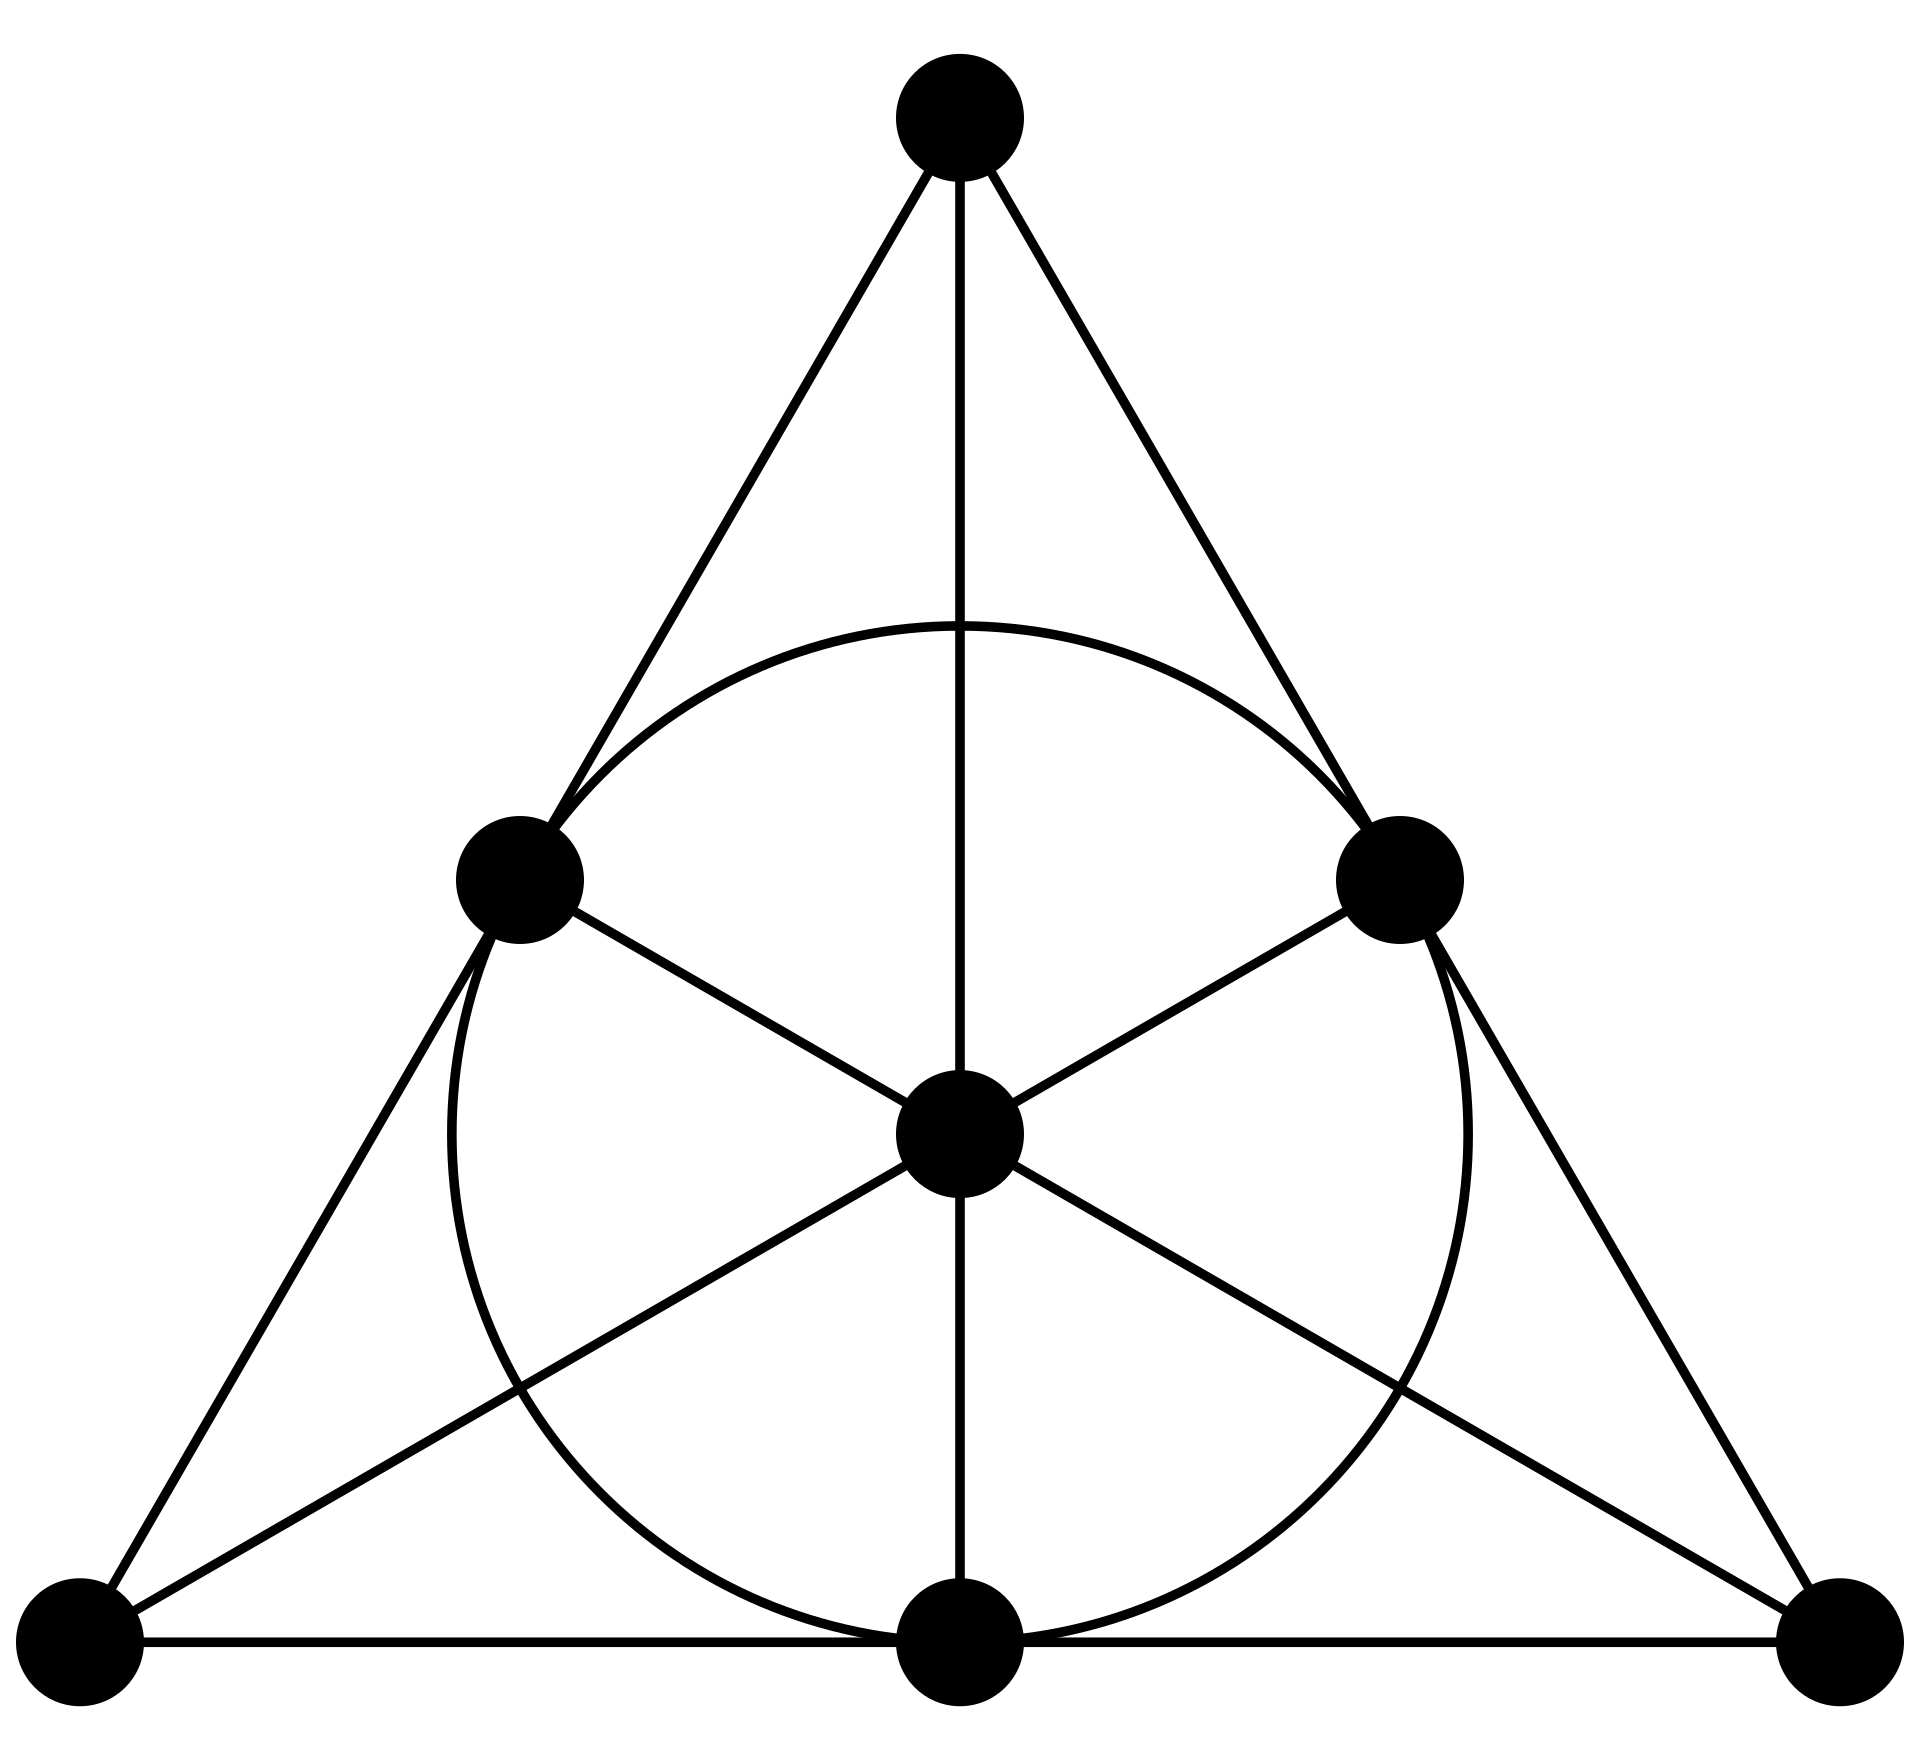
\includegraphics[scale=0.1]{images/fano_plane.png}
		\caption{The Fano plane.}
	\end{center}
\end{figure}
We get plenty of examples for dimension greater than $2$ by taking projective space over a field or division ring. These are all of the examples of projective space in these dimensions. The difference between fields and division rings is that being in a field means that \index{Pappus's theorem}Pappus's theorem holds.

\subsection{Desargues's theorem.}
\begin{theorem}[Desargues]\label{}\index{Desargues's theorem}
If the three straight lines joining the corresponding vertices of two triangles $ABC$ and $\tilde A\tilde B\tilde C$ all meet in a point (the perspector), then the three intersections of pairs of corresponding sides lie on a straight line (the perspectrix). Equivalently, if two triangles are perspective from a point, they are perspective from a line.\footnote{Weisstein, Eric W. ``Desargues's Theorem.'' From {MathWorld}---A Wolfram Web Resource. \url{https://mathworld.wolfram.com/DesarguesTheorem.html}.}
\end{theorem}

It is useful to think about these triangles in space. One sees that $AB$ and $\tilde A\tilde B$, $AC$ and $\tilde A\tilde C$, and $BC$ and $\tilde B\tilde C$ do meet. These three points all lie on the planes containing $ABC$ and $\tilde A\tilde B\tilde C$, so they lie on the intersection of these two planes, which is typically a line. ``So, if these triangles are not both contained in the same plane, then Desargues's theorem holds and, if they are contained in the same plane, then you can mumble something about taking limits and still deduce the theorem.''

A projective space automatically satisfies this theorem if it has dimension at least $3$. However, there are some cases in which projective planes do not satisfy it. These counterexamples are called non-Desarguesean planes. In some sense, Desargues's theorem is equivalent to associativity of multiplication. One can introduce coordinates to form a ring for a projective space, and it turns out that the truth of Desargues's theorem is equivalent to associativity holding in the ring, just as Pappus's theorem is equivalent to commutativity. An example of a non-Desarguesean plane is a projective plane over a non-associative ring such as the octonions.\footnote{That is, synthetic projective geometry is almost analytic projective geometry, but not quite.}

One has duality for projective space, too. Any two distinct points meet in a line, and any two distinct lines meet in a point. That is, points are dual to lines: anything you can say about lines and points you can say about points and lines. There is a dual to Pascal's theorem. 

One can think about this as duality of vector spaces. Points in projective space $\mathbf{P}^n$ correspond to lines in $\mathbf{A}^{n+1}$, which one thinks about as $K^{n+1}$. Lines in $\mathbf{P}^n$ correspond to planes in $K^{n+1}$. Consider the dual space $(K^{n+1})^*$ which is (non-canonically) isomorphic to $K^{n+1}$. The dual of a line in $\mathbf{A}^{n+1}$ is a hyperplane consisting of all linear transformations vanishing on it. So, lines correspond to hyperplanes, planes corresponds to things of codimension $2$, etc., so hyperplanes correspond to lines, which are points of projective space.

\subsection{Affine varieties. Projective varieties.}
Recall that affine space $\mathbf{A}^n$ corresponds to its coordinate ring $K[z_1,\hdots, z_n]$. An affine algebraic subset corresponds to a radical ideal $I=\mathfrak{r}({I}) $.

Projective space sort of corresponds to $K[z_0,\hdots, z_n]$ where one considers this a graded ring that is graded in the obvious way. Projective algebraic sets correspond to graded radical ideals in which every element is a sum of homogeneous elements in the ideal.\footnote{This correspondence ignores the ideal $(z_0,\hdots, z_n)$.} 

A cone over a projective variety in $\mathbf{P}^n$ sort of corresponds to an affine variety in $\mathbf{A}^{n+1}$ that is invariant under rescaling.

Projective space is affine space together with points at infinity.
\begin{example}[ ]\label{}
Consider the affine variety $y=x^3$. To make this into a projective variety, instead of considering $(x,y) \in \mathbf{A}^2$, we consider $(x:y:z)\in \mathbf{P}^2$. The affine point $(x,y)$ corresponds to the projective point $(x:y:1)$. One needs a homogenous polynomial, and one is $yz^2 = x^3$. What does this variety look like?

Well, $\mathbf{P}^2$ is covered by $3$ copies of affine space, so one can take either $x\ne 0$, $y\ne 0$, or $z\ne 0$. In each case, we scale the nonzero component to make it $1$. If $x=1$, we have $(y,z)$, if $y=1$, we have $(x,z)$, and, if $z=1$, we have $(x,y)$. In the case $z=1$, one gets the curve we had before: $y=x^3$. In the case $y=1$, one gets $z^2 = x^3$. In the case $x=1$, one gets $yz^2 = 1$. One can imagine these three curves, but how do they fit together? 

If one takes the point $(1,1)$ on the first curve, this corresponds to $(1:1:1)$ in projective space, which corresponds to $(1,1)$ on the other two curves. The point $(0,0)$ corresponds to $(0:0:1)$. On the second curve, one wants to rescale such that $y=1$, but one can't, so this corresponds to a point at infinity, and so it is with the third (here, the point at infinity in the ``rightward'' direction). Now, consider the point $(0,0)$ on the second curve. Again, this corresponds to a point at infinity on the first curve and the other point at infinity on the third one. All other points are on all three curves. Notice that this curve has a singularity at a point at infinity.
\end{example}

\begin{example}[ ]\label{}
Consider the elliptic curve $y^2 = x^3+bx+c$. This is the affine representation. In the projective plane, one has three coordinates $(x:y:z)$, and one needs to make this homogeneous, so one gets $y^2z = x^3 + bxz^2 + cz^3$. In the case $z\ne 0$, one gets the same curve: $y^2 = x^3 + bx + c$. In the case $z=0$, one gets $x=0$, so the only point at infinity is the point $(0:\lambda:0)$. What does the curve look like near this point? Is this singular?

For this, one considers the case $y=1$, so one gets $z = x^3 + bxz^2 + cz^3$. The point at infinity in the original curve is the point $(0,0)$ here. If $x$ and $z$ are small, then $z$ is $x^3$ plus something small, so, around $(0,0)$, one gets something that looks like $z=x^3$. Therefore, it is nonsingular, so the projective curve is nonsingular at the point at infinity.
\end{example}

\begin{example}[ ]\label{}
Consider $y^2 = x^2 + 1$. Looking at the curve, one sees that the curve tends to a point where $x$ and $y$ are large and equal to the right, corresponding to $(1:1:0)$. One gets another point $(1:-1:0)$. These are points at infinity. A straightforward check corroborates this.
\end{example}

\begin{example}[Twisted cubic]\label{}
The \index{twisted cubic}twisted cubic is the set of points of the form $(t,t^2,t^3)$. The ideal that defines this curve is $(y-x^2, z-x^3)$. What is its closure in projective space $\mathbf{P}^3$?

Here's the wrong answer: Take generators for the ideal and make them homogeneous: We get $ (wy-x^2,w^2z-x^3)$, which is a graded ideal in $K[w,x,y,z]$ and defines something in $\mathbf{P}^3$. The first ideal contains things like $y^2-zx$, but this second one doesn't (it also doesn't contain $z-xy$). In projective space, the closure of the twisted cubic is given by $(s^3:s^2t:st^2:t^3)$ (the curve above where $s=1$ and another point where $s=0$). The ideal of polynomials vanishing on this is $(wy-x^2, y^2-zx, wz- xy)$. What happens if you take the incorrect set of generators for the closure of the twisted cubic?

That is, what happens when one takes $(wy-x^2, w^2z - x^3) \subset K[w,x,y,z]$? What algebraic set in $\mathbf{P}^3$ does it define? Projective space $\mathbf{P}^3$ is covered by four copies of affine space $\mathbf{A}^3$, corresponding to $w=1$, $x=1$, $y=1$, and $z=1$. In the case $w=1$, one gets the twisted cubic with which we started. In the case $x=1$, one gets $wy=1$ and $w^2z = 1$, which is a copy of the affine $z$-line minus a point (the original curve minus a point). In the case $y=1$, one gets $w=x^2$ and $w^2z=x^3$, so $x^3(zx-1)=0$. Hence, one has a curve $zx=1$, which corresponds to the original curve and a triple line where $x=0=w$. That is, when one makes this na\"ive choice of generators, one picks up something strange at infinity.

That this contains two components corresponds to the following decomposition:
\begin{align*}
	(wy-x^2, w^2z - x^3) = (wy-x^2,y^2-xz, wz-xy) \cap  (wy-x^2, w^2, wx).
\end{align*}
\end{example}

\subsection{Products of varieties.}
Clearly, one has
\begin{align*}
	\mathbf{A}^m \times \mathbf{A}^n = \mathbf{A}^{m+n}
\end{align*}
where $((z_1,\hdots,z_m),(y_1,\hdots,y_n))\longmapsto  (z_1,\hdots, z_m,y_1,\hdots, y_n)$. In terms of coordinate rings, this is $K[z_1,\hdots,z_m]\tensor_K K[y_1,\hdots, y_n]$, which is. more or less, $K[z_1,\hdots, z_m,y_1,\hdots, y_m]$. Suppose that $X$ and $Y$ are algebraic sets with corresponding ideals $I$ and $J$. Then, $X\times Y$ corresponds to the ideal $(I,J)$.

Notice:
\begin{align*}
	\mathbf{P}^m \times \mathbf{P}^n\ne \mathbf{P}^{m+n}.
\end{align*}
This isn't true even topologically: $\mathbf{P}^1_{\mathbf{R}}\times \mathbf{P}^1_{\mathbf{R}}\isomto S^1\times S^1$ is the torus, while $\mathbf{P}^2_{\mathbf{R}}$ is non-orientable. Similarly, $\mathbf{P}^1_{\mathbf{C}}\times \mathbf{P}^1_{\mathbf{C}}\isomto S^2\times S^2$ whose second homology group is $\HH^2(S^2\times S^2) =  \mathbf{Z}\oplus \mathbf{Z}$, while $\mathbf{P}^2_{\mathbf{C}}$ is the union of a point, $\mathbf{C}$, and $\mathbf{C}^2$ whose second homology group is $\mathbf{Z}$. While the convenient equality doesn't hold between these two objects, they are birational.

Let's try to map $((z_0:\cdots:z_m), (y_0:\cdots:y_n))\longmapsto (z_0:\cdots:z_m:y_1:\cdots:y_n)$. This isn't even well defined. To get such a map, one needs everything to be of the same degree in $z$ and $y$:
\begin{align*}
	((z_0:\cdots:z_m), (y_0:\cdots:y_n))\longmapsto (z_0y_0:z_1y_0:\cdots:z_my_0:\cdots: z_0y_1:\cdots:z_my_n).
\end{align*}
This produces the non-surjective map $\mathbf{P}^m\times \mathbf{P}^n\longrightarrow \mathbf{P}^{mn+m+n}$ whose image is a closed subset. Write an element in the image $(w_{00}:w_{10}:\cdots: w_{m0} : \cdots: w_{mn})$. One has some relations: $w_{ij} = x_iy_j$, so $w_{ij}w_{pq}=w_{iq}w_{pj}$. 

Suppose that one has $v\in K^{m+1}$ and $w\in K^{n+1}$. Then, one has $v\tensor w \in K^{m+1}\tensor K^{n+1}$. This is, more or less, the map above.

One wants to show that the map from $\mathbf{P}^m\times \mathbf{P}^n$ to vectors $(w_{00}:\cdots:w_{mn})$ satisfying $w_{ij}w_{pq}=w_{iq}w_{pj}$ is surjective. One assumes that $w_{00}=1$ without loss of generality. Then, $w_{pq} = w_{0q}w_{p0}=y_qx_p$. Thus, the $w_{pq}$s are determined by $ w_{0q}$ and $w_{p0}$. One can fix these to be whatever one wants by choosing $z$ and $y$ correctly, assuming $z_0=y_0=1$. Therefore, this map, called the \index{Segre embedding}Segre embedding, is surjective.

\begin{example}[Segre embedding]\label{seg}
One has
\begin{align*}
	\mathbf{P}^1\times \mathbf{P}^1\longrightarrow \mathbf{P}^{1+1+1}
\end{align*}
given by $((z_0:z_1), (y_0:y_1)) \longmapsto (z_0y_0:z_0y_1: z_1y_0: z_1y_1) =:(w_0:w_1:w_2:w_3)$. One gets one relation: $w_0w_3=w_1w_2$. This is a quadric in $\mathbf{P}^3$. Over an algebraically closed field with characteristic not $2$, any two nonsingular quadrics are isomorphic. That is, any quadric in $\mathbf{P}^3$ is isomorphic to $\mathbf{P}^1\times \mathbf{P}^1$. In particular, it has two sets of lines on it. 

Suppose one takes a sphere $x^2+y^2+z^2=1$. One claims that this has two sets of straight lines on it. Indeed, it does over $\mathbf{C}$. Example: $x=1$, $y=iz$. Exercise: Find all straight lines on this sphere over $\mathbf{C}$.\footnote{Writing this as $(x+iy) (x-iy)= (1-z) (1+z)$ puts into the form of the quadric above.}
\end{example}


\subsection{The Veronese surface. The variety of lines in space.}

\begin{example}[Veronese surface]\label{}
\index{Veronese surface} The Veronese surface is given by
\begin{align*}
	(x^2:xy:xz:y^2:yz:z^2)\in  \mathbf{P}^5.
\end{align*}
One can think of this as a map $\mathbf{P}^2\longrightarrow \mathbf{P}^5$ where
\begin{align*}
	(x:y:z) \longmapsto (x^2:xy:xz:y^2:yz:z^2).	
\end{align*}
This is clearly not surjective. Write this point as $(w_{00}:w_{01}:w_{02}:w_{11}:w_{12}:w_{22})$. One has $w_{ij}w_{pq} = w_{ip}w_{jq}$. Accounting for these relations, the map is surjective. One can also think of this as a map $\mathbf{A}^3\longrightarrow \mathbf{A}^6$ where $\mathbf{A}^6 = \Sigma^2\mathbf{A}^3$ is thought of as the symmetric square of $\mathbf{A}^3$. Note that $\dim \Sigma^2\mathbf{A}^n = n(n+1)/2$. One can also consider maps $\mathbf{A}^3\longrightarrow \Sigma^3 \mathbf{A}^3$ and $\mathbf{A}^m \longrightarrow \Sigma^n \mathbf{A}^m$. The images of these maps are \index{Veronese variety}Veronese varieties.
\end{example}

\begin{example}[Variety of lines in $\mathbf{P}^3$]\label{}
We expect this variety to be of dimension $4$. A line in $\mathbf{P}^3$ corresponds to a two-dimensional subspace of $K^4$. This is a special case of a \index{Grassmannian}Grassmannian. A Grassmannian $\Gr(m,n)$ is the set of $m$-dimensional subspaces of the vector space $K^{m+n}$. The Grassmannians $\Gr(0,m)=\Gr (m,0)$ are points. The Grassmannian $\Gr(1,m)$ is projective space $\mathbf{P}^m$. Finally, $\Gr(m,n)\isomto \Gr (n,m)$. The first is an $m$-dimensional subspace of $K^{m+n}$; its dual $(K^{m+n})^*\isomto K^{m+n}$ gives an $n$-dimensional subspace. So $\Gr(m,1)\isomto \Gr(1,m)$. The first nontrivial case of this is $\Gr(2,2)$, which comprises the two-dimensional subspaces of $K^4$.

Grassmannians are special cases of \index{Hilbert scheme}Hilbert schemes: Schemes whose points correspond to certain configurations (algebraic sets, subschemes) of projective space satisfying certain conditions; the simplest condition is that this should be a linear subspace.

We would like to make $\Gr(2,2)$ a projective variety. We shall embed $\Gr(2,2)$ into $\mathbf{P}^5$. Pick a line in $\mathbf{P}^3$ which corresponds to a point of $\Gr(2,2)$. Pick two points $(a_0:a_1:a_2:a_3)$ and $(b_0:b_1:b_2:b_3)$ on the line. Consider the matrix
\begin{align*}
	\mat{a_0&a_1&a_2&a_3\\b_0&b_1&b_2&b_3}.
\end{align*}
Let $S_{ij}$ be the determinant of the columns $i$ and $j$. We get $(S_{01}:S_{02}:S_{03}:S_{12}:S_{13}:S_{23}) \in \mathbf{P}^5$. This point depends on only the line. The map we get is not surjective, since $\Gr(2,2)$ is dimension $4$ and $\mathbf{P}^5$ is dimension $5$. Therefore, there must be a relation between these determinants. This is the \index{Plucker relation}Plucker relation:
\begin{align*}
	S_{01}S_{23}-S_{02}S_{13}+S_{03}S_{12}=0.
\end{align*}
There are no other relations.

We want to show that the map from $\Gr(2,2)$ to solutions to the Plucker relation is surjective. Some $S_{ij}$ must be nonzero, so we can assume it is $1$. Without loss of generality, assume that $S_{01}=1$. Then $S_{01}S_{23}$ is some combination of the other determinants, and $S_{23}$ is determined by them. We get a matrix
\begin{align*}
	\mat{1&0&-S_{12}&-S_{13}\\0&1&S_{02}&S_{03}}
\end{align*}
which gives a line in $\Gr(2,2)$ with image a given point of $\mathbf{P}^5$.
\end{example}

One can use this to find the cohomology of a quadric in $\mathbf{P}^5_{\mathbf{C}}$. The Grassmannian is a union of subsets:
\begin{align*}
	&\mat{1&0&*&*\\0&1&*&*};
	\quad\mat{1&*&0&*\\0&0&1&*};\\
	&\mat{1&*&*&0\\0&0&0&1};
	\quad\mat{0&1&0&*\\0&0&1&*};\\
	&\mat{0&1&*&0\\0&0&0&1};
	\quad\mat{0&0&1&0\\0&0&0&1}.
\end{align*}\iffalse
\begin{align*}
	&\mat{0&0&1&0\\0&0&0&1}.
\end{align*}
\fi
These correspond to $\mathbf{A}^4$, $\mathbf{A}^3$, $\mathbf{A}^2$, $\mathbf{A}^2$, $\mathbf{A}^1$, and $\mathbf{A}^0$ respectively. One also uses this to determine how many points $\Gr(2,2)$ has over a finite field $K$. If $q=\left\lvert K \right\rvert $, then $\Gr(2,2)$ has $q^0 + q^1 + 2q^2 + q^3+q^4$ points. One sees that $\mathbf{P}^4$ has $q^0+q^1+q^2+q^3+q^4$ points.

This strongly suggests there is a relationship between the cohomology groups of a variety over $\mathbf{C}$ and the number of points of that variety over a finite field. This is the concern of the Weil conjectures.

\subsection{Grassmannians.}
The Grassmannian $\Gr(2,2)$ can be thought of as the two-dimensional subspaces of $K^4$, or, alternatively, lines in space. Grassmannians $\Gr(m,n)$ are injective maps $K^m \longrightarrow K^{m+n}$.
One can show that
\begin{align*}
	\Gr(m,n) \subseteq  \mathbf{P}^{\mathscr{C}({m+n},{m})-1}.
\end{align*}

Suppose we are given an $m$-dimensional subspace of $K^{m+n}$. Pick $m$ vectors spanning it. This gives an $m\times(m+n)$ matrix:
\begin{align*}
	\mat{a_1&\cdots &a_{m+n}\\b_1&\cdots &b_{m+n}\\&\vdots}.
\end{align*}
Pick any $m$ columns and consider the determinant of these columns. This generates $\mathscr{C}({m+n},{m})$ numbers. Call them $p_{{i_1},\hdots,{i_m}}$. These give a point in $\mathbf{P}^{\mathscr{C}({m+n},{m}) - 1}$. 

Instead, suppose that $V\subseteq W$ is a subspace of $W$ with with dimension $m$. Suppose $W$ has dimension $m+n$. Then, one has a map from the $m$th exterior power of $V$ to the $m$th exterior power of $W$:
\begin{align*}
	\bigwedge\nolimits^m V \longrightarrow  \bigwedge\nolimits ^m W.
\end{align*}
The first space has dimension $1$ and the second space has dimension $\mathscr{C}({m+n},{m})$. A one-dimensional subspace of something corresponds to the projective line over that thing: $\mathbf{P}_{\bigwedge\nolimits^m W}$. This map is not surjective. 
One has the Plucker relations:
\begin{align*}
	0 &= \sum_{\lambda}^{} (-1)^\lambda p_{i_1,\hdots, i_{m-1},j_\lambda} p_{j_1,\hdots, j_{\lambda -1},j_{\lambda+1},\hdots, j_{m+1}}.
\end{align*}
These give quadric relations that make the map from $\Gr(m,n)$ to the roots of the Plucker relations surjective. We can assume, say, that $p_{1,\hdots, m} = 1$. Then, we can find a point of $\Gr(m,n)$ with given values of $p_{1,\hdots, r-1,r+1,\hdots, m,s}$. The Plucker relations determine all of the other $p$s.

Grassmannians have applications.
\begin{enumerate}
	\item Grassmannians are covered by affine spaces that can be used to determine their cohomologies.
	\item One has the Littlewood--Richardson rule\index{Littlewood--Richardson rule} that gives the product of the cohomology of a Grassmannian.
	\item One has \index{line complex}line complexes. One constructs the quadric line complex by taking $\Gr(2,2)\subset  \mathbf{P}^5$ and intersecting it with a quadric.
	\item The Grassmannian $\Gr(m,n)$ is a quotient 
		\[
			{\GL_{m+n}(K)}/{\mat{*&*\\0&*}}.
		\] 
		Both members of the quotient are affine, but the resulting Grassmannian is not affine.\footnote{It is projective.} Quotients of affine varieties do not need to be affine or projective: Take 
		\begin{align*}
			K^2 - \{(0,0)\} =  {\GL_{2}(K) }/{\mat{1&*\\0&1}}.
		\end{align*}
	\item Grothendieck used Grassmannians in his construction of Hilbert schemes. A \index{Hilbert scheme}Hilbert scheme parameterizes subschemes of projective space. Take the coordinate ring $K[z_0,\hdots, z_n]$ of projective space and consider graded ideals $I = \bigoplus_j I_j$. Subschemes sort of correspond to graded ideals, so one tries to classify graded ideals and show that they correspond to points of a projective scheme. The dimension $\dim (I_j)$ is a polynomial in $j$ for $j$ large. Suppose that $I_d$ generates $I_{d+1},I_{d+2},\hdots$. Then $I_d \subseteq S_d$ (degree-$d$ monomials). This gives a point of a Grassmannian, which is itself a projective variety in a larger projective space.
\end{enumerate}

One would like to say that lines in $\mathbf{P}^3$ ``naturally'' correspond to points of $\Gr(2,2)\subset  \mathbf{P}^5$. 
\begin{quote}
	\small What does ``natural'' mean?
\end{quote} 
Grothendieck looked at functors from commutative rings $R$: Maps $F$ from $R$ to lines in $\mathbf{P}^3(R)$, maps from $R$ to $\Gr(2,2)$ over $R$, maps $G$ from $R$ to $R$-valued points of a quadric given by the Plucker relation. Grothendieck showed that these are isomorphic as functors. 

Suppose $\phi: R\longrightarrow  S$ is a ring homomorphism. Then, we have maps $F(R) \longrightarrow F(S)$ and $G(R) \longrightarrow G(S)$ that make this commute:
\[
\begin{tikzcd}
F(R) \arrow[d, -,double equal sign distance,double]\arrow[r] &F(S) \arrow[d, -,double equal sign distance,double] \\ G(R)\arrow[r] & G(S).
\end{tikzcd}
\]
Grothendieck showed that any scheme is defined by its functor of points.

\subsection{Projective space bundles.}
Recall the definition of a fibre bundle: A fibre bundle\index{fibre bundle} is a space that looks like a product locally. Specifically, a fibre bundle is a structure $(E,B, \pi, F)$ where $E$, $B$, and $F$ are topological spaces and $\pi:E\longrightarrow B$ is a continuous surjective map that, in small regions of $E$, behaves like a projection from $B\times F$ to $B$. For sufficiently small open sets $U$,
\begin{center}
	\begin{tikzcd}
		F \ar[r] & E\ar[d] & F\times U \ar[d]\\
			 &B&U\ar[l,hook']
	\end{tikzcd}
\end{center}
commutes.

Take $B=S^1$ and $F=\mathbf{R}$. Then, we can map $S^1\times \mathbf{R}$ onto $S^1$, which would look like a cylinder mapping onto a circle with fibres copies of $\mathbf{R}$. One can twist this construction, mapping a M\"obius strip onto $S^1$. One can think of the fibres as copies of $\R$. Locally, this looks like a product: The preimage of a little section of the circle looks like $\R$ times that little section.

Fibre bundles are ``twisted products.'' Often, the fibre is a vector space; in this case, we talk about a \index{vector bundle}vector bundle. If the fibre is a copy of projective space, we talk about a \index{projective space bundle}projective space bundle.

\begin{example}[Hirzebruch surface]\label{}
\index{Hirzebruch surface}Consider the space
\begin{align*}
	(\mathbf{A}^2 - \{0\})^2 = (\mathbf{A}^2 - \{0\}) \times (\mathbf{A}^2 - \{0\}).
\end{align*}
Act on this by $G\textsubscript{m}\times G\textsubscript{m}$.\footnote{For now, $G\textsubscript{m}$ is $\mathbf{C}^*$.} The quotient $(\mathbf{A}^2 - \{0\})/G\textsubscript{m}$ where $\lambda \in G\textsubscript{m}$ acts by $(z_1,z_2)\longmapsto  (\lambda z_1,\lambda z_2)$ is the projective line $\mathbf{P}^1$. Pick a point $(\lambda,\mu)\in  G\textsubscript{m}\times G\textsubscript{m}$; now, act on a point $(s,t,z_1,z_2)$ by
\begin{align*}
	(s,t,z_1,z_2)\longmapsto  (\lambda s, \lambda t,\mu z_1,\lambda^{-\alpha}\mu z_2),\ \alpha\in  \mathbf{Z}.
\end{align*}
The quotient defined by this action is a Hirzebruch surface. One has a map
\begin{align*}
	F := (\mathbf{A}^2-\{0\})^2/({G\textsubscript{m}\times G\textsubscript{m}})\longrightarrow \mathbf{P}^1
\end{align*}
given by
\begin{align*}
	(s,t,z_1,z_2)\longmapsto  (s:t).
\end{align*}
The fibre at any point is also isomorphic to $\mathbf{P}^1$. Locally, this is a product, but it isn't globally. One has a surface that is a fibre bundle over $\mathbf{P}^1$ with fibres in $\mathbf{P}^1$.
\end{example}

\begin{example}[Scrolls]\label{}
\index{scroll}
Act on the space $(\mathbf{A}^2-\{0\})^2$ by $G\textsubscript{m}\times G\textsubscript{m}$ where $(\lambda,\mu)$ acts on $(s,t,z_1,\hdots, z_n)$ by 
\begin{align*}
	(s,t,z_1,\hdots,z_n)\longmapsto  (\lambda s, \lambda t, \lambda^{-\alpha_1}\mu z_1,\hdots, \lambda^{-\alpha_n}\mu z_n), \ \alpha_i\in \mathbf{Z}.
\end{align*}
One gets a map from the scroll to the projective line
\begin{align*}
	{(\mathbf{A}^2-\{0\})^2}/({G\textsubscript{m}\times G\textsubscript{m}}) \longrightarrow \mathbf{P}^1
\end{align*}
given by
\begin{align*}
	(s,t,z_1,\hdots, z_n) \longmapsto (s:t).
\end{align*}
Here, the fibres are copies of $\mathbf{P}^{n-1}$. Grothendieck showed that, if one has a vector bundle over the projective line,  one can replace each vector space that is a fibre with the corresponding vector space, and this gives a projective bundle over $\mathbf{P}^1$. This construction covers all such vector bundles.

Let us map this to projective space. Assume that $\alpha_i>0$. Consider the monomials $s^it^{\alpha_j-1}z_j$. One can take these as the coordinates of a point in $\mathbf{P}^{\left( \sum_{}^{} \alpha_j+1 \right) - 1}$.
\end{example}

\index{abstract variety}Abstract varieties were invented by Andr\'e Weil to take the Jacobian of a curve to formulate his Weil conjectures. A differentiable manifold was viewed as a subset of $\mathbf{R}^n$ defined by some equations. For instance, $S^2$ is the set of points $x^2+y^2+z^2=1$ in $\mathbf{R}^3$. However, this isn't a differentiable manifold, really; it is a differentiable manifold together with an embedding into Euclidean space. Now, one covers $S^2$ with charts\index{chart}: A top hemisphere and a bottom hemisphere, each of which looks like an open disk in Euclidean space, glued together. 

The old view was that a variety is a subset of $\mathbf{P}^n$ defined by equations. The new one follows: Take some affine varieties and glue them together. One might have considered $\mathbf{P}^1$ as a subset of projective space (itself). Alternatively, one can glue together two copies of $\mathbf{A}^1$, so $\mathbf{P}^1=\mathbf{A}^1\cup \mathbf{A}^1$. The projective line is given by $(z_1:z_2)$, the first copy of $\mathbf{A}^1$ is given by $(1:z_2)$, and the second is given by $(z_1:1)$. For both copies, one considers the subset $\mathbf{A}^1-\{0\}$. Then, if one has $z_1$ in the first copy and $z_2$ in the second, one maps
\begin{align*}
	z_1\longmapsto \frac{1}{z_2}.
\end{align*}
The ``gluing'' given by $z_1\longmapsto z_2$ is kind of funny: One gets a line with two origins.\footnote{This is a non-Hausdorff manifold and a non-projective abstract variety.} If one eliminates this phenomenon, all dimension-$1$ abstract varieties are projective. One needs to exclude singularities in dimension $2$. There are some abstract nonsingular non-projective varieties in dimension $3$. \index{Chow's lemma}Chow's lemma says that an abstract complete variety is pretty close to a projective variety. 

\subsection{Toric varieties.}
\index{toric variety}Toric varieties give an easy way to construct examples of projective varieties.

\begin{example}[Constructing affine varieties from cones: Dimension $2$]\label{}
Consider the coordinate ring of $K^*\times K^*$, namely $K[z_1,z_1^{-1},z_2,z_2^{-1}]$. One gets a square lattice of monomials. One defines subrings by drawing cones:
\begin{center}
	\phantom{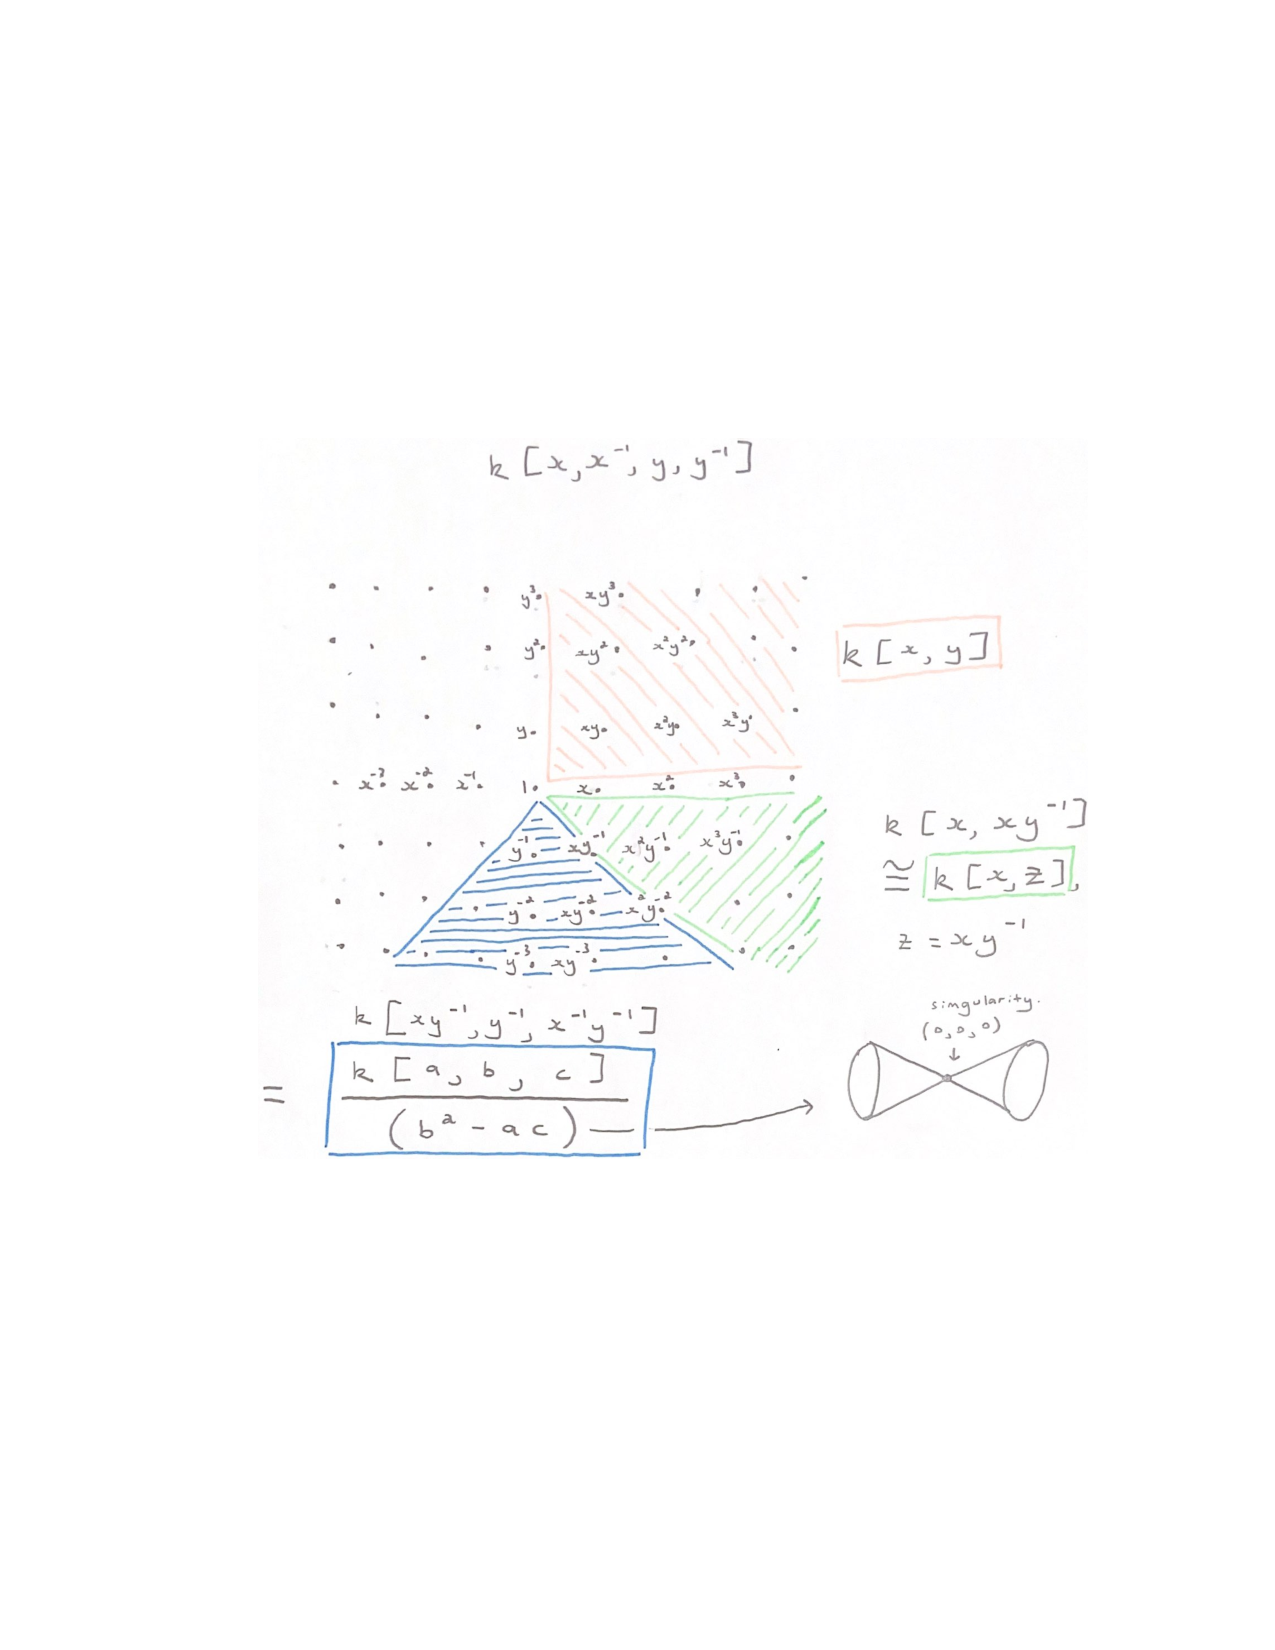
\includegraphics[scale=0.8]{images/subring_cone.pdf}}
\end{center}
A subring given by a cone has the following properties:
\begin{enumerate}
	\item It is a $K$-algebra;
	\item It has no nilpotent elements;
	\item If the cone is rational, it is a finitely-generated algebra.
\end{enumerate}
If these three conditions are met, this gives the coordinate ring of an affine variety. The orange and green cones correspond to $\mathbf{A}^2$ and the blue cone corresponds to a double cone as drawn above. 

Suppose we have an orange cone and a larger red cone that contains the orange cone. One sees that the orange ring is a subring of the red ring. Since we have a map from the orange ring to the red ring, we have a map from the red variety to the orange variety. We can get around this problem using duality. 

If one has a cone in $\mathbf{Z}^2$, one can look at the dual cone: the corresponding cone in $(\mathbf{Z}^2)^*=\mathbf{Z}^2$. The orange dual cone contains the red dual cone. The idea: For each cone $C$ in $\mathbf{Z}^2$, look at the dual cone and take the corresponding ring. This gives a variety of $C$.

Consider a degenerate cone (a vertical line). The dual of this cone is the upper half plane. The coordinate ring of this is $K[z_1,z_1^{-1},z_2]$, which corresponds to $K^*\times K$. This is the ring corresponding to the line.

Consider a quadrant. Its dual is the same quadrant whose coordinate ring is $K[z_1,z_2]$, so this corresponds to the affine plane or $K\times K$. Now, one sees that sub--- is preserved under taking coordinate rings of cones.\footnote{That is, $K^*\times K$ is a subring of $K\times K$ and, correspondingly, the line is a subcone of the quadrant.}
\end{example}

		One can do the same with more cones. Consider the following cones in $1$ dimension: An upward line at the origin, a downward line at the origin, and their intersection (a point). The lines are self-dual, but the dual of the point is the entire line. The lines correspond to $K[z]$ and $K[z^{-1}]$ respectively, thus $\mathbf{A}^1$, and the point corresponds to $K[z,z^{-1}]$, thus $\mathbf{A}^1 - \{0\}$. Take these affine varieties and glue them together. One gets $\mathbf{P}^1$. 


Now, in two dimensions, take four distinct quadrants. One gets four varieties which are isomorphic to $\mathbf{A}^2$. We are gluing them together along various subvarieties. The right horizontal one corresponds to $\mathbf{A}^2 - \mathbf{A}^1 = \mathbf{A}^1 \times (\mathbf{A}^1 - \{0\})$. The picture one has is just two copies of the picture one had in the one-dimensional case, so one gets $\mathbf{P}^1\times \mathbf{P}^1$. The variety $\mathbf{P}^1 \times \mathbf{P}^1$ as a toric variety is drawn like this. How does one get $\mathbf{P}^2$?

Consider these cones:
\begin{center}
	\phantom{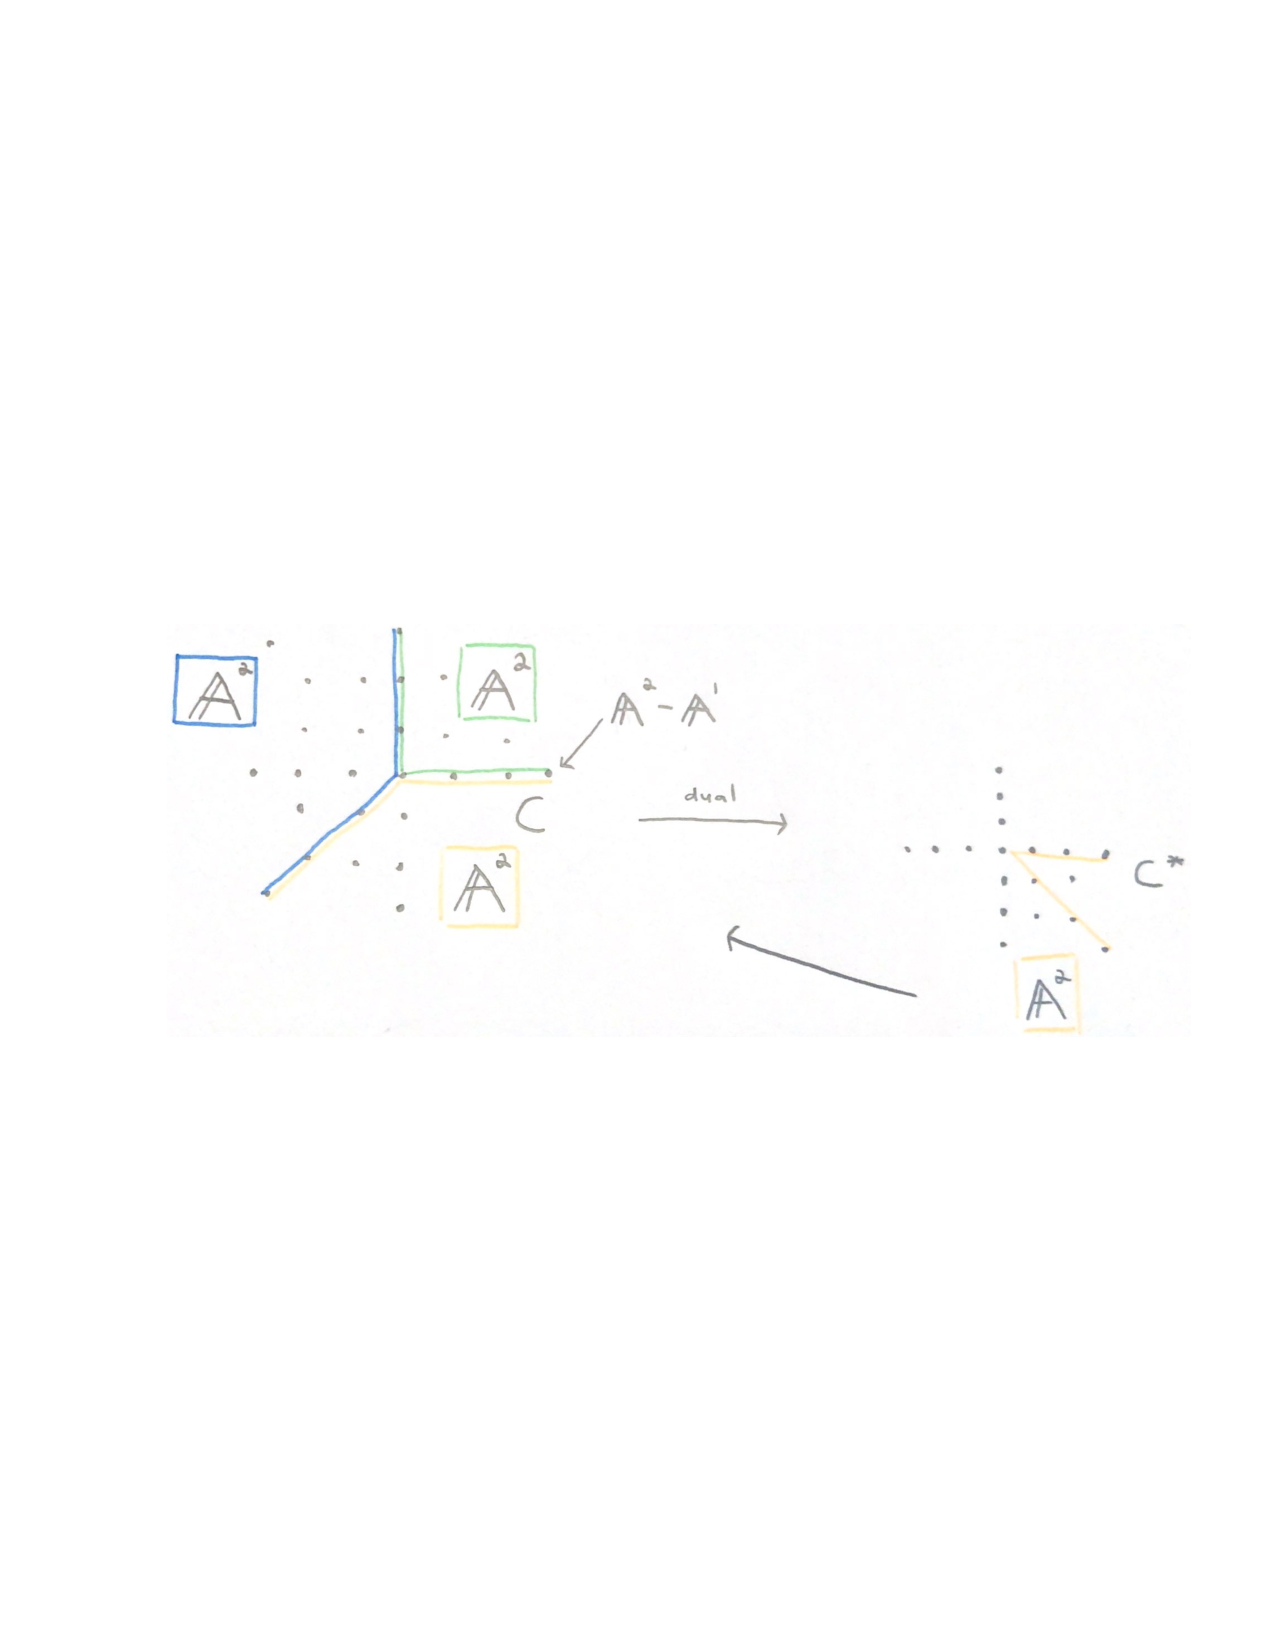
\includegraphics[scale=0.8]{images/toric_proj_plane.pdf}}
\end{center}
Looking at the dual cone, one sees that the orange and blue cones correspond to $\mathbf{A}^2$.  Again, one sees that the green and orange cones are glued together by the variety $\mathbf{A}^2 - \mathbf{A}^1$. So $\mathbf{P}^2$ is $\mathbf{A}^2\cup \mathbf{A}^2\cup \mathbf{A}^2$ glued along copies of $\mathbf{A}^1\times (\mathbf{A}^1-\{0\})$.

Consider this more exotic example:
\begin{center}
	\phantom{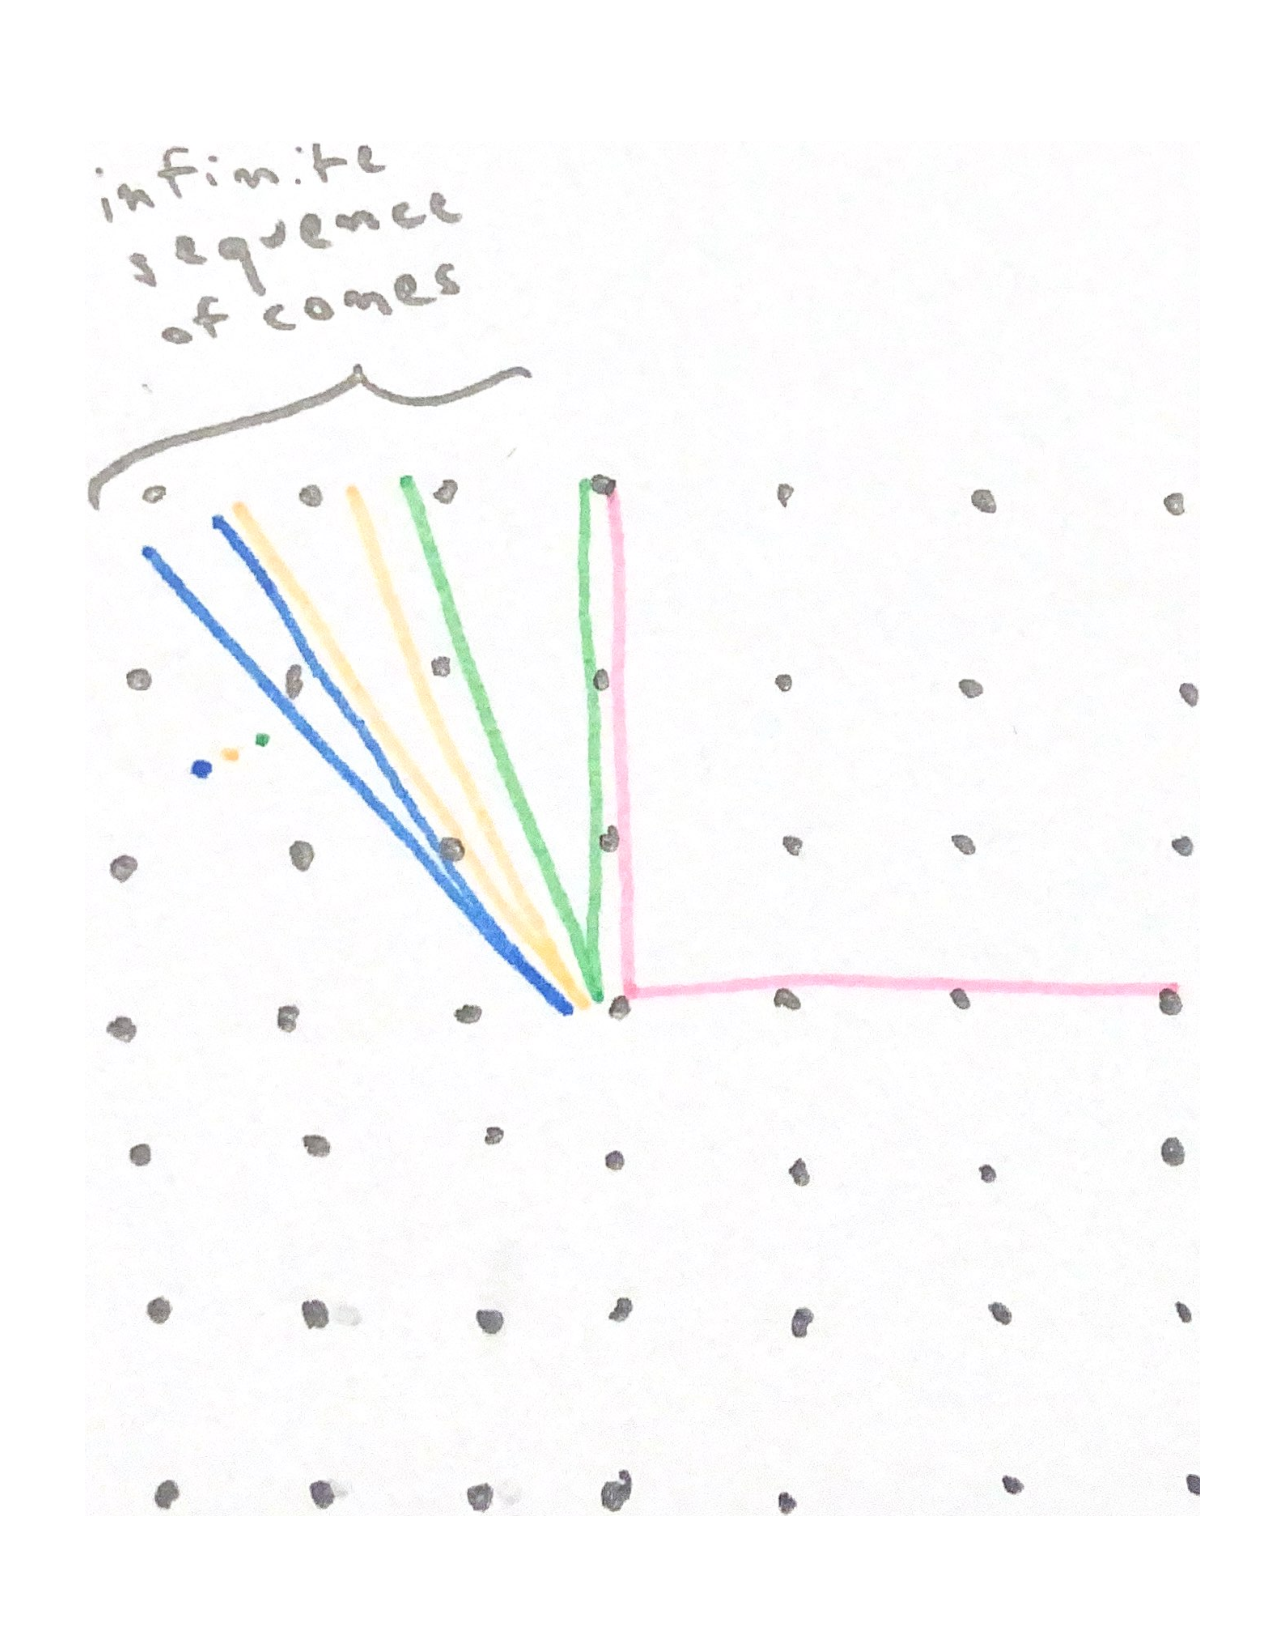
\includegraphics[scale=0.4]{images/cone_seq}}
\end{center}
One can take an infinite sequence of cones and glue together copies of $2$-dimensional affine space according to this sequence. What projective variety does one get? Well, one doesn't get one: It is too big. The resulting thing is not \index{quasicompact}quasicompact, and all projective varieties or their open subsets are quasicompact. Instead, it gives an \index{abstract variety}abstract variety. Varieties one gets like this are called toric varieties: They contain a torus as a dense subvariety.

In the drawing above, notice that there is a single point contained in all of the cones. The variety of this point is, looking at the dual cone, $K[z_1,z_1^{-1},z_2,z_2^{-1}]$. This is the coordinate ring of a torus. Why is this called a ``torus''?

One knows that, in algebraic topology, a torus is $S^1\times S^1$, or, more generally, $(S^1)^n$. Over $\mathbf{R}$, $S^1$ is the set of points $x^2 + y^2 = 1$. Over $\mathbf{C}$, this is $(x+iy) (x-iy)=1$ or $z_1z_2=1$. This is a hyperbola, which is $\mathbf{C}-\{0\}$. Hence, one can think of $\mathbf{C}^*$ as an analogue of $S^1$. Therefore, one can call $(\mathbf{C}^*)^n$ a torus. In the theory of algebraic groups, $(\mathbf{C}^*)^n$ plays the same role that $(S^1)^n$ plays is the theory of compact Lie groups. 

\subsection{Categories.}
A category has objects and morphisms. They are named after their objects. Here are some examples.
	\begin{center}
\begin{tabular}{lr}
    Objects & Morphisms\\
    \midrule
    Sets & Functions\\
    Groups & Group homomorphisms\\
    Topological spaces & Continuous maps\\
    Commutative rings & Ring homomorphisms
\end{tabular}
\end{center}
A category has a collection of objects. For any two objects, one has a collection of morphisms between them. Given objects $A$, $B$, and $C$, a morphism $f$ from $A$ to $B$, and a morphism $g$ from $B$ to $C$, one has a morphism $g\circ f$ from $A$ to $C$. For every object $A$, there is an identity morphism $I_A$. This identity must behave as one expects. Composition of morphisms must be associative when defined.

A theme of category theory is to focus on morphisms between objects, and not the objects themselves. How does one define products? The definitions of products of sets, groups, topological spaces, etc. are notably different. Suppose $A$ and $B$ are two objects. Suppose $C$ is another object with morphisms to $A$ and $B$. Then there is a unique morphism from $C$ to $A\times B$. This is universal:
\begin{center}
	\begin{tikzcd}
		C \ar[ddr] \ar[dr, dashed] \ar[drr] \\
		& A\times B \ar[r] \ar[d] & B\\
		& A
	\end{tikzcd}
\end{center}
One can check that products of sets, groups, rings, topological spaces, etc. satisfy this universal property. The product is not unique but it is unique up to unique isomorphism.

Suppose $X$ and $Y$ both satisfy the universal property above. Since $Y$ is a product and $X$ maps to $A$ and $B$, there is a unique map from $X$ to $Y$ that makes the diagram commute. Reverse the roles of $X$ and $Y$ to get a unique map from $Y$ to $X$. The composition of these two unique morphisms is a map from $Y$ to itself that makes the diagram commute; by unicity, this morphism must be the identity of $Y$. Reverse the roles of $X$ and $Y$.

We would like to make varieties or algebraic sets into a category. One can use \index{regular map}regular maps, which are somewhat analogous to smooth maps in differential geometry and defined everywhere, or one can use \index{rational map}rational maps, which are not defined everywhere.

Given a category $\mathscr{C} $, its opposite $\mathscr{C}\op$ is $\mathscr{C} $ with all arrows reversed. The morphisms of ${\mathscr{C}}\op $ from $A$ to $B$ are the same as the morphisms of $\mathscr{C} $ from $B$ to $A$. Affine varieties with regular maps is somewhat dual to finitely-generated algebras over $K$ with no nilpotent elements.\footnote{Affine schemes have the same correspondence to commutative rings.}

A map of varieties $V\longrightarrow W$ does not give a map from a coordinate ring of $V$ to that of $W$; it gives a map from functions on $W$ to functions on $V$.


\subsection{Regular functions.}
An affine variety $Y\subseteq \mathbf{A}^n$\index{affine variety} is defined by an ideal $I$ and the coordinate ring of $Y$ is $K[z_1,\hdots,z_n]/I$, which one thinks of as polynomial functions on affine space restricted to $Y$. This coordinate ring is the \index{ring of regular functions}ring of regular functions on $Y$.

We would like to define regular functions when $U$ is an open subset of an affine variety $Y$. Such open sets are called \index{quasiaffine variety}quasiaffine varieties.

\begin{example}[Quasiaffine varieties]\label{}
Take $U=\mathbf{A}^1-\{0\}$. We have seen that $U$ is isomorphic to the hyperbola of points $xy=1$ in $\mathbf{A}^2$. This quasiaffine variety is an affine variety disguised.

Take $U=\mathbf{A}^2-\{(0,0)\}$. We will see that this is not isomorphic to an affine variety.
\end{example}

What does one want the regular functions on $U$ to be? If $U=\mathbf{A}^1-\{0\}$, one wants $z^{-1}$ to be regular on $U$. Hence, one wants the ring to be $K[z,z^{-1}]$. One defines a regular function\index{regular function} on $U$ to be a function that is locally regular at all points $p\in U$.\footnote{A function $f$ is \index{locally regular}locally regular at $p$ if $f=g/h$ in some neighbourhood of $p$ where $g$ and $h$ are polynomials and $h$ is nonzero at $p$. Note that $g$ and $h$ depend on $p$.}

\begin{problem}
	Suppose that $Y$ is affine. Are regular functions regular? Note that the first ``regular'' means ``regular at each point'' and the second means that they are polynomials on affine space.
\end{problem}

Suppose $Y=U_1\cup U_2\cup \cdots \cup U_m$ is a union of open subsets. Let $f$ be a function on $Y$ that is regular on all $U_i$s. Therefore, $f=g_i/h_i$ on $U_i$ where $h_i\ne 0 $ on $U_i$. Is $f$ a polynomial? Observe that $1= a_1h_1 + a_2h_2 + \cdots +a_mh_m\pmod I$ for some polynomials $a_i$. This is because $Y$ is covered by the $U_i$s; thus, no point of $Y$ is outside of all $U_i$s, and no maximal ideal of $K[z_1,\hdots,z_n]$ containing $I$ contains all of the $h_i$s; so $(h_1,\hdots, h_m, I)=(1)$. This relation gives
\begin{align*}
	f &= a_1h_1f + a_2h_2f + \cdots + a_mh_mf \pmod I\\
	  &= a_1g_1 + a_2g_2+\cdots + a_mg_m \pmod I.
\end{align*}
Define $f:= a_1g_1+\cdots + a_mg_m$. We want to check that $h_if = g_i$ on $U_i$: Since $h_if = h_ia_1g_1 +\cdots + h_ia_mg_m$ and $h_ig_j = h_jg_i$, one gets
\begin{align*}
	h_if &= h_ia_1g_1 +\cdots + h_ia_mg_m\\
	     &= g_ia_1h_1 + \cdots + g_ia_mh_m\\
	     &= g_i(a_1h_1+\cdots+a_mh_m)\pmod I\\
	     &= g_i \pmod I.
\end{align*}
Therefore, the local and global conditions for regularity are equivalent.

Suppose that $U$ is a \index{quasiprojective variety}quasiprojective variety, so it is an open subset of a projective variety.\footnote{Every quasiaffine variety is a quasiprojective variety.} Notice that a quasiprojective variety is covered by open affine subvarieties. A function on a quasiprojective variety is  \index{regular function}regular if it is \index{locally regular}locally regular.

Given a quasiprojective variety $Y$, one has a \index{ring of regular functions}ring of regular functions $\mathscr{O}(U)$ for each open subset $U\subset Y$. 

Suppose that $U= U_1\cup U_2\cup \cdots$. One has the following properties:
\begin{enumerate}
	\item If $f\in \mathscr{O}(U) $ vanishes on $\mathscr{O}(U_i) $, then $f = 0$;
	\item If $f_i\in \mathscr{O}(U_i) $ and $f_i = f_j$ on $U_i\cap U_j$, then there exists $f\in \mathscr{O}(U) $ such that $f \big |_{U_i} = f_i$.
\end{enumerate}
These are the defining conditions of a \index{sheaf}sheaf.

\begin{example}[ ]\label{}
Let us find the regular functions on $\mathbf{P}^1$. The regular functions on $\mathbf{A}^1$ is $K[z]$. We cover the projective line with two copies of the affine line: $\mathbf{P}^1 = \mathbf{A}^1\cup \mathbf{A}^1$. To specify a regular function $f\in \mathbf{P}^1$, pick regular functions on $\mathbf{A}^1$ and $\mathbf{A}^1$ that are the same on the intersection $\mathbf{A}^1-\{0\}$. The ring of regular functions on $\mathbf{A}^1-\{0\}$ is $K[z,z^{-1}]$. One can identify the ring of regular functions of the second copy of $\mathbf{A}^1$, $K[y]$, with $K[z^{-1}]$. One needs to pick $f$ that is a polynomial in $z$ and a function that is a polynomial in $z^{-1}$ that are the same in $K[z,z^{-1}]$. Thus, $f$ is constant.
\end{example}

\subsection{Morphisms of varieties.}
Suppose that $X$ and $Y$ are quasiprojective varieties. We want to define a regular map $f:X\longrightarrow Y$. This should be a ``nice'' function from points of $X$ to points of $Y$. ``Nice'' functions from $\eta:Y\longrightarrow K$ are regular functions, so the composition $\eta\circ f$ should be regular.

Suppose $U$ is open in $Y$. Then $f^{-1}(U)$ is open in $X$. Let $g: U\longrightarrow K$ be a regular function. Then $f$ is called a morphism if the composition $g\circ f$ is regular on $f^{-1}(U)$. Indeed, the composition of two morphisms is a morphism. Quasiprojective varieties and this morphism comprise a category.

\begin{warn}
	This is a morphism of \index{ringed space}ringed spaces. A \defn{ringed space}\index{ringed space} is a topological space with a sheaf of rings. We have seen that regular functions on open sets form a sheaf of rings. This definition fails for schemes: One needs to use a morphism of locally ringed spaces.
\end{warn}

\begin{example}[Ringed spaces]\label{}
	 Topological manifolds: Take continuous functions on every open set. Then, one can take $C^1$ manifolds, $C^2$ manifolds, etc., and $C^\infty$ manifolds (smooth manifolds), in which the ringed space structure is given by smooth functions on every open set. Continuing, one can take analytic manifolds $C^\omega$, and then smooth algebraic varieties over $\mathbf{C}$ or $\mathbf{R}$. These are more or less inclusions. Topological manifolds are ``floppy,'' while smooth algebraic varieties are ``rigid.'' There is a significant change in behaviour between smooth manifolds and analytic manifolds.  

	 All of these are \index{locally ringed space}locally ringed spaces.
\end{example}

Suppose $X$ is a topological space together with a sheaf of rings. For each open set $U$ of $X$, we have a ring $\mathscr{O}(U)$. If we have open sets $U\subseteq V$, we have a restriction map $\mathscr{O} (U)  \longleftarrow \mathscr{O}(V)$. The local ring\index{local ring} at a point $\mathfrak{p}\in X$ is, informally, ``functions defined near $\mathfrak{p}$.'' More precisely, an element of a local ring is given by an open set $U$ such that $\mathfrak{p}\in U$ and a function $f\in \mathscr{O}(U)$ defined on $U$. We define an equivalence relation by $(f,U)\sim  (g,V)$ if there exists $W\subseteq U\cap V$ and $\mathfrak{p}\in W$  so $f=g$ on $W$. The set of equivalence classes is a ring called the \index{local ring}local ring at $\mathfrak{p}$. Indeed, this is a local ring with maximal ideal functions vanishing at $\mathfrak{p}$.

\begin{example}[ ]\label{}
Consider the hyperbola $xy=1$ and the points $\mathbf{A}^1-\{0\}$. We can define a morphism from the hyperbola by $(x,y)\longmapsto x$ and one in the other direction by $x\longmapsto (x,x^{-1})$. These maps are inverses of each other, so these two objects are isomorphic in the category of quasiprojective varieties.
\end{example}

\begin{example}[ ]\label{}
Consider the curve $C: y^2=x^3$. There is a map $\mathbf{A}^1\longrightarrow C$ given by $t\longmapsto (t^2,t^3)$. This morphism of varieties is a continuous bijection, so it an isomorphism of sets. Further, its inverse is continuous, so it is a homeomorphism of topological spaces. However, it is not an isomorphism of varieties. We might try to define $t = y/x$, but this is not regular at $x=0$.
\end{example}

\subsection{Affine algebraic sets and commutative rings.}
\begin{theorem}[ ]\label{}\index{}
Suppose $Y$ is affine. Then morphisms $X\longrightarrow Y$ are the same as ring homomorphisms $\mathscr{O}(Y)  \longrightarrow \mathscr{O}(X)$.
\end{theorem}

\begin{proof}
Suppose $\varphi \in \Mor(X,Y)$. This gives a ring homomorphism from $\mathscr{O}(Y) $ to $\mathscr{O}(X)$. An element of $\mathscr{O}(Y)$ is a regular function, just some $\psi\in \Mor(Y, \mathbf{A}^1)$, and this will map to $\psi\circ\varphi$. This works for all $Y$. The problem is constructing a map from $\Hom_{}(\mathscr{O}(Y), \mathscr{O}(X))$ to $\Mor(X,Y)$. 

Suppose $h\in \Hom_{}(\mathscr{O}(Y),\mathscr{O}(X) )$. Think of $\mathscr{O}(Y)$ as $K[z_1,\hdots, z_n]/I$ for some ideal $I$ since $Y$ is affine. Construct $\psi:X\longrightarrow Y$ as follows: For $p\in X$, one has $(h(z_1)(p),\hdots, h(z_n) (p))\in K^n$. This defines a map $X\longrightarrow \mathbf{A}^n$, which is $\psi$. One needs to check that the image of $\psi$ is in $Y$, and this follows from $h(I)=0$. Also, one needs to check that $\psi$ is a morphism, and this follows from $x_i\circ\psi$ being regular on $X$.

The two functions defined above are inverses of each other.
\end{proof}
\begin{remark}
This means that affine varieties over $K$ are ``the same as'' finitely-generated $K$-algebras with no nilpotent elements. That is, the category of affine varieties over $K$ is dually equivalent to the category of finitely-generated $K$-algebras.

Therefore, products of varieties correspond to coproducts of algebras. The coproduct is the dual of the product:
\begin{center}
        \begin{tikzcd}
                T \\
                & R\tensor S \ar[ul, dashed] & R\ar[l]\ar[llu]\\
                & S\ar[u] \ar[uul]
        \end{tikzcd}
\end{center}
\end{remark}
\begin{warn}
	This fails over non-perfect fields: If $L$ is an inseparable extension of $K$, then $K\tensor_L K$ might have nilpotent elements. 
\end{warn}

\begin{example}[Algebraic groups]\label{}
An \defn{algebraic group}\index{algebraic group} $G$ is an algebraic variety together with a morphism $G\times G\longrightarrow G$ (a ``product'') with an ``inverse'' morphism $G\longrightarrow G$ and an ``identity'' morphism from a point to $G$. The variety $\mathbf{A}^1$ with product
\begin{align*}
	(z_1,z_2)\longmapsto z_1+z_2
\end{align*}
is an algebraic group $G\textsubscript{a}$ with inverse
\begin{align*}
	z\longmapsto -z
\end{align*}
and identity $0$. Now, let us look at this from the point of view of rings. The coordinate ring of $\mathbf{A}^1$ is $K[z]$ and the coordinate ring of $\mathbf{A}^1\times \mathbf{A}^1$ is $K[z_1]\tensor K[z_2]$. The corresponding homomorphism is $z\longmapsto z_1+z_2$. That is, we have two maps: $K[z]\tensor K[z]\longrightarrow K[z]$, which is ring multiplication, and $K[z]\longrightarrow K[z]\tensor K[z]$, which is the group operation. These look dual (cf. \index{Cartier duality}Cartier duality).
\end{example}

\begin{example}[The multiplicative case: $G\textsubscript{m}$]\label{}
Here, the underlying variety is $\mathbf{A}^1 - \{0\}$ with group ring $K[z,z^{-1}]$ and product 
\begin{align*}
	(z_1,z_2)\longmapsto z_1\cdot z_2.
\end{align*}
The coproduct $K[z,z^{-1}] \longrightarrow K[z,z^{-1}]\tensor K[z,z^{-1}]$ is given by 
\begin{align*}
	z\longmapsto z\tensor z.
\end{align*}
\end{example}

\begin{example}[$\GL_2(K)$]\label{}
Here, the product is given by matrix multiplication and the inverse is given by the ordinary inverse. The coordinate ring is 
\[
	R:=K[a,b,c,d,(ad-bc) ^{-1}].
\] 
One can think of this as 
\[
	{K[a,b,c,d,e]}/{((ad-bc)e-1)}.
\] 
One has a homomorphism of rings $R\longrightarrow R\tensor R$ corresponding to the product where $a\longmapsto a_1a_2+b_1c_2$, etc. according to matrix multiplication. The inverse corresponds to a homomorphism of rings $R\longrightarrow R$ taking each entry to the appropriate entry of the inverse. These are called {Hopf algebras}\index{Hopf algebra}: Things with a multiplication $R \longrightarrow  R\tensor R$, a comultiplication $R\tensor R\longrightarrow R$, and an antipode corresponding to the inverse and satisfying some axioms.
\end{example}

\begin{definition}
The data $(B,\nabla, \eta,\Delta,\varepsilon)$ give a $K$-\defn{bialgebra}\index{bialgebra} if and only if the following conditions hold.
\begin{enumerate}
	\item $B$ is a $K$--vector space.
	\item There exists a $K$-linear map, a so-called ``multiplication,'' $\nabla : B\tensor B \longrightarrow B$ (equivalently, a $K$-multilinear map $\nabla:  B\times B\longrightarrow B$) and a so-called ``unit'' $\eta : K\longrightarrow B$ such that the data $(B, \nabla, \eta)$ comprise a unital associative algebra. 
	\item There exists a $K$-linear map, a so-called ``comultiplication,'' $\Delta  :B \longrightarrow B\tensor B$ and a so-called ``counit'' $\varepsilon : B\longrightarrow K$ such that the data $(B,\Delta, \varepsilon)$ comprise a counital coassociative coalgebra. 
	\item The diagram
	\begin{center}
	\begin{tikzcd}[row sep = 4 em, column sep = 4 em]
		B\tensor B \ar[r, "\nabla"] \ar[d, "\Delta\tensor \Delta", swap] & B\ar[r,"\Delta"] & B\tensor B\\
		B\tensor B\tensor B\tensor B \ar[rr, "\id\tensor \tau\tensor \id", swap] && B\tensor B\tensor B\tensor B\ar[u, "\nabla\tensor\nabla", swap]
	\end{tikzcd}
\end{center}
commutes where $\tau :B\tensor B\longrightarrow B\tensor B $ is given by $\tau (x\tensor y) = y\tensor x$.
\item The diagram
\begin{center}
	\begin{tikzcd}[row sep = 3 em, column sep = 3 em]
		B\tensor B \ar[rr, "\nabla"] \ar[dr, "\varepsilon\tensor\varepsilon", swap] &&B\ar[dl, "\varepsilon"]\\
		&K\tensor K\isomto K
	\end{tikzcd}
\end{center}
commutes.
\item The diagram
\begin{center}
	\begin{tikzcd}[row sep = 3 em, column sep = 3 em]
		& K\tensor K\isomto K \ar[dr, "\eta"] \ar[dl, "\eta\tensor \eta", swap] \\
		B\tensor B &&B\ar[ll,"\Delta"]
	\end{tikzcd}
\end{center}
commutes.
	\item The diagram
\begin{center}
	\begin{tikzcd}[row sep = 3 em, column sep = 3 em]
		& B \ar[dr, "\varepsilon"]\\
		K\ar[rr,"\id", swap] \ar[ur, "\eta"]&&K
	\end{tikzcd}
\end{center}
commutes.
\end{enumerate}
\end{definition}


\begin{definition}
A $K$-bialgebra $(B,\nabla, \eta,\Delta,\varepsilon)$ is a \defn{Hopf algebra}\index{Hopf algebra} if and only if there exists a $K$-linear function 
\[
	\alpha : B\longrightarrow B,
\]
the so-called ``antipode,'' such that
\[
	\nabla \circ(\id\tensor \alpha) \circ \Delta = \nabla \circ (\alpha\tensor \id) \circ \Delta = \eta\circ \varepsilon.
\]
\end{definition}



\subsection{The twisted cubic.}
We shall look at some examples of morphisms of varieties.

\begin{example}[Twisted cubic]\label{}
\index{twisted cubic}The twisted cubic is isomorphic to $\mathbf{P}^1$. Recall that the twisted cubic is given by points of the form $(w:x:y:z) = (s^3:s^2t:st^2:t^3)\in  \mathbf{P}^3$. One can also describe it as the roots of $wy=x^2$, $xz=y^2$, and $wz=xy$. We get a graded ring $K[w,x,y,z]$ modulo these polynomials.

One has an isomorphism from $\mathbf{P}^1$ to the twisted cubic given by 
\begin{align*}
	(s:t) \longmapsto  (s^3:s^2t:st^2:t^3).
\end{align*}
This is an isomorphism of topological spaces. However, this might not be an isomorphism of algebraic sets. So we need to construct a regular map from the twisted cubic to $\mathbf{P}^1$. Cover the cubic with open affine sets $U_i$. Choose a function on each $U_i$ and check that they are the same on $U_i\cap U_j$.

Projective space $\mathbf{P}^3$ is covered by four copies of $\mathbf{A}^3$, corresponding to the cases $w\ne 0$, $x\ne 0$, $y\ne 0$, and $z\ne 0$. The twisted cubic is covered by $2$ affine sets given by $w\ne 0$ and $z\ne 0$. For $w\ne 0$, we map
\begin{align*}
	(w:x:y:z)\longmapsto  (w:x).
\end{align*}
For $z\ne 0$, we map
\begin{align*}
	(w:x:y:z)\longmapsto  (y:z).
\end{align*}
For the intersection ($w\ne 0$ and $z\ne 0$), recall that $wz=xy$, so $(w:x)= (y:z)$, and, hence, we have a regular morphism from the cubic to $\mathbf{P}^1$. Indeed, this is the inverse of the map we gave earlier.
\end{example}

\begin{remark}
	Two affine varieties are isomorphic if and only if the corresponding coordinate rings are isomorphic. The same statement is false for projective varieties and the corresponding graded rings: The graded ring corresponding to $\mathbf{P}^1$---namely, $K[z_1,z_2]$---and the graded ring corresponding to the twisted cubic are certainly not isomorphic.
\end{remark}

\begin{example}[ ]\label{}
Recall that $\mathbf{A}^1-\{0\}$ is affine, while $\mathbf{A}^2 - \{(0,0)\}$ is not. Let us find the regular functions on $\mathbf{A}^2 - \{(0,0)\}$ (morphisms from it to $\mathbf{A}^1$). Cover $\mathbf{A}^2-\{(0,0)\}$ by affine sets $U$ and $V$. Let $U$ be $\mathbf{A}^2$ without the $x$ axis and $V$ be $\mathbf{A}^2$ without the $y$ axis. The corresponding coordinate rings are $K[z_1,z_2,z_2^{-1}]$ and $K[z_1,z_1^{-1},z_2]$. The intersection $U\cap V$ has coordinate ring $K[z_1,z_1^{-1},z_2,z_2^{-1}]$. We have maps from $U\cap V$ to $U$ and from $U\cap V$ to $V$ that induce dual maps of the coordinate rings. These corresponding maps are injective, so finding elements in either ring with the same image in $K[z_1,z_1^{-1},z_2,z_2^{-1}]$ is straightforward: One gets $K[z_1,z_2]$ for the regular functions on $\mathbf{A}^2-\{(0,0)\}$. This is the same as the coordinate ring of $\mathbf{A}^2$.

The inclusion $\mathbf{A}^2-\{(0,0)\}\longrightarrow \mathbf{A}^2$ induces a map $K[z_1,z_2] \longleftarrow K[z_1,z_2]$. Since morphisms of affine varieties correspond to homomorphisms of coordinate rings, if $\mathbf{A}^2-\{(0,0)\}$ were affine, then $K[z_1,z_2]$ would be its coordinate ring. Since the homomorphism here is an isomorphism, $\mathbf{A}^2-\{(0,0)\}$ would have to be isomorphic to $\mathbf{A}^2$. Hence, $\mathbf{A}^2-\{(0,0)\}$ is not affine.
\end{example}

\begin{remark}
	With $\mathbf{A}^1-\{0\}$, one is removing a subset of codimension $1$; with $\mathbf{A}^2-\{(0,0)\}$, one is removing a subset of codimension $2$. Roughly, if one removes a subset of codimension $1$ from an affine variety, it generally remains affine; this does not tend to happen for codimension greater than $1$.
\end{remark}


\subsection{Products of projective varieties.}
Suppose $A\subseteq \mathbf{P}^m$ and $B\subseteq \mathbf{P}^n$ are varieties. If we can find a product $\mathbf{P}^m\times \mathbf{P}^n$, it is not hard to find a product $A\times B$. We shall demonstrate that the product of two projective varieties is projective.

Recall that \index{Segre embedding}we have the Segre embedding:
\begin{align*}
	\mathbf{P}^m\times \mathbf{P}^n\longrightarrow \mathbf{P}^{mn+m+n}.
\end{align*}
We want to find that the image is a product in the category of varieties. This embedding is given by
\begin{align*}
	((x_0:\cdots:x_m), (y_0:\cdots:y_n))\longmapsto (x_0y_0:x_1y_0:\cdots:x_my_0:\cdots: x_0y_1:\cdots:x_my_n).
\end{align*}
Write $(z_{00}:\cdots:z_{mn}):=(x_0y_0:x_1y_0:\cdots:x_my_0:\cdots: x_0y_1:\cdots:x_my_n)$. We have the relations
\begin{align*}
	z_{ij}z_{k\ell} = z_{i\ell}z_{kj}.
\end{align*}

Let us check that there is a morphism from the variety given by those relations to projective space. Suppose $z_{00}\ne 0$. Then we have a map from the Segre variety to $\mathbf{P}^m$ by
\begin{align*}
(z_{00}:\cdots:z_{mn})\longmapsto (z_{00}:z_{10}:\cdots:z_{m0})\in \mathbf{P}^m.	
\end{align*}
If $z_{01}\ne 0$, we have a similar map given by
\begin{align*}
	(z_{00}:\cdots:z_{mn})\longmapsto (z_{01}:z_{11}:\cdots:z_{m1})\in \mathbf{P}^m.
\end{align*}
Do these maps coincide intersect on the intersection of the two open subsets? Yes: We have the relations $z_{ij}z_{k\ell} = z_{i\ell}z_{kj}$. 

Let $S$ be the Segre variety. If $C$ is a variety that maps to $\mathbf{P}^m$ and $\mathbf{P}^n$, we want to show that there is a unique map $C\longrightarrow S$:
\begin{center}
        \begin{tikzcd}
                C \ar[ddr] \ar[dr, dashed] \ar[drr] \\
                & S \ar[r] \ar[d] & \mathbf{P}^n\\
                & \mathbf{P}^m
        \end{tikzcd}
\end{center}
Cover $C$ by open affine varieties. If we have proved this works for affine varieties, we get maps from each open affine variety to $S$. By the unicity of the maps for the product, all of the maps must coincide on all of the intersections. Hence, one assumes that $C$ is affine without loss of generality.

One also covers the projective spaces by open affine varieties. A morphism from $C$ to the open subset $\{x_0\ne 0\}$ of $\mathbf{P}^m$ is given by a set of regular functions on $C$: $\{f_0=1,f_1,\hdots, f_m\}$. Similarly, one from $C$ to the open subset $\{y_0\ne 0\}$ of $\mathbf{P}^n$ is given by $\{g_0=1,g_1,\hdots, g_n\}$. 

In general, an affine variety will not map to the open subset $\{x_0\ne 0\}$ of $\mathbf{P}^m$. However, one can cover $C$ by smaller open subsets where each open subset maps to one of the standard open subsets of $\mathbf{P}^m$ and one of $\mathbf{P}^n$. Thus, one also assumes that the image of $C$ is in the open subset $\{x_0\ne 0\}$ of $\mathbf{P}^m$.\footnote{And similarly for $\mathbf{P}^n$.}

Now, we have a map 
\begin{align*}
	C\longrightarrow (f_0g_0:f_0g_1:\cdots:f_mg_n).
\end{align*}
One checks that this is well-defined, etc.

\subsection{Automorphisms of space.}
\begin{problem}
	What is the group of automorphisms of an algebraic set?
\end{problem}

Automorphism groups of algebraic sets tend to be trivial or uninteresting. However, affine and projective space happen to be quite symmetric.

\begin{example}[Automorphisms of the affine line]\label{}
The coordinate ring of $\mathbf{A}^1$ is $K[z]$, so morphisms $\mathbf{A}^1\longrightarrow \mathbf{A}^1$ correspond to algebra homomorphisms $K[z]\longrightarrow K[z]$ (that is, $z\longmapsto \rho(z)$). Therefore, morphisms from $\mathbf{A}^1$ to itself are polynomials with coefficients in $K$. These are invertible if $\rho(z) = az+b$ for $a\ne 0$. Therefore, $\Aut(\mathbf{A}^1)$ is the $az+b$ group, and one can identify this with
\begin{align*}
	\left\{ \mat{a&b\\0&1} \right\}. 
\end{align*}
This group is nonabelian and has a normal subgroup 
\begin{align*}
	\left\{\mat{ 1&b\\0&1} \right\} 
\end{align*}
isomorphic to the additive group $K$.\footnote{And whose quotient is isomorphic to the multiplicative group $K^*$.}
\end{example}

\begin{example}[Automorphisms of the affine plane]\label{}
The coordinate ring of $\mathbf{A}^2$ is $K[z_1,z_2]$. Some automorphisms include 
\begin{align*}
	(z_1,z_2)\longmapsto (az_1+bz_2+c, dz_1+ez_2+f) 
\end{align*}
where
\begin{align*}
	ae - bd \ne 0.
\end{align*}
The invertible map
\begin{align*}
	(z_1,z_2)\longmapsto  (z_1,z_2+\rho(z_1))
\end{align*}
is an automorphism. Hence, we have an infinite-dimensional abelian subgroup. One can do the same with $z_1$, consider compositions, etc. 
\end{example}

\begin{example}[Automorphisms of affine space]\label{}
Consider this endomorphism of $\mathbf{A}^n$:
\begin{align*}
	z_i\longmapsto f_i(z_1,\hdots, z_n).
\end{align*}
When is this an automorphism? Consider the Jacobian determinant $\det (\partial f_i/\partial z_j)$. One has
\begin{align*}
	\det (\Jac FG) =  (\det \Jac F) (\det \Jac G).
\end{align*}
Therefore, if $FG = 1$, then $\det\Jac F$ is invertible. One conjectures that this is an automorphism if and only if the Jacobian is invertible. One direction is trivial, and the other is the \index{Jacobian conjecture}Jacobian conjecture: If $\det \Jac F$ is invertible then $F$ is an automorphism. This is open.
\end{example}

\begin{example}[Automorphisms of the projective line]\label{}
One can restrict a map $\mathbf{P}^1\longrightarrow \mathbf{P}^1$ to a map $\mathbf{A}^1\longrightarrow \mathbf{P}^1$, and this gives a map from an open subset of $\mathbf{A}^1$ to $\mathbf{A}^1$. Hence, we have a regular map on an open subset of $\mathbf{A}^1$ given by a rational function $p(z)/q (z)$. These have inverses if they are of the form
\begin{align*}
	\frac{az+b}{cz+d}\textrm{\quad where\quad$ad - bc \ne 0$.}
\end{align*}
However, the matrix $\alpha I$ corresponds to the identity, so one needs to mod out by things of this form. This gives $\PGL_2(K)$, which is of dimension $3$. This is parallel to what one sees in complex analysis.
\end{example}
\iffalse
\begin{figure}
\begin{center}
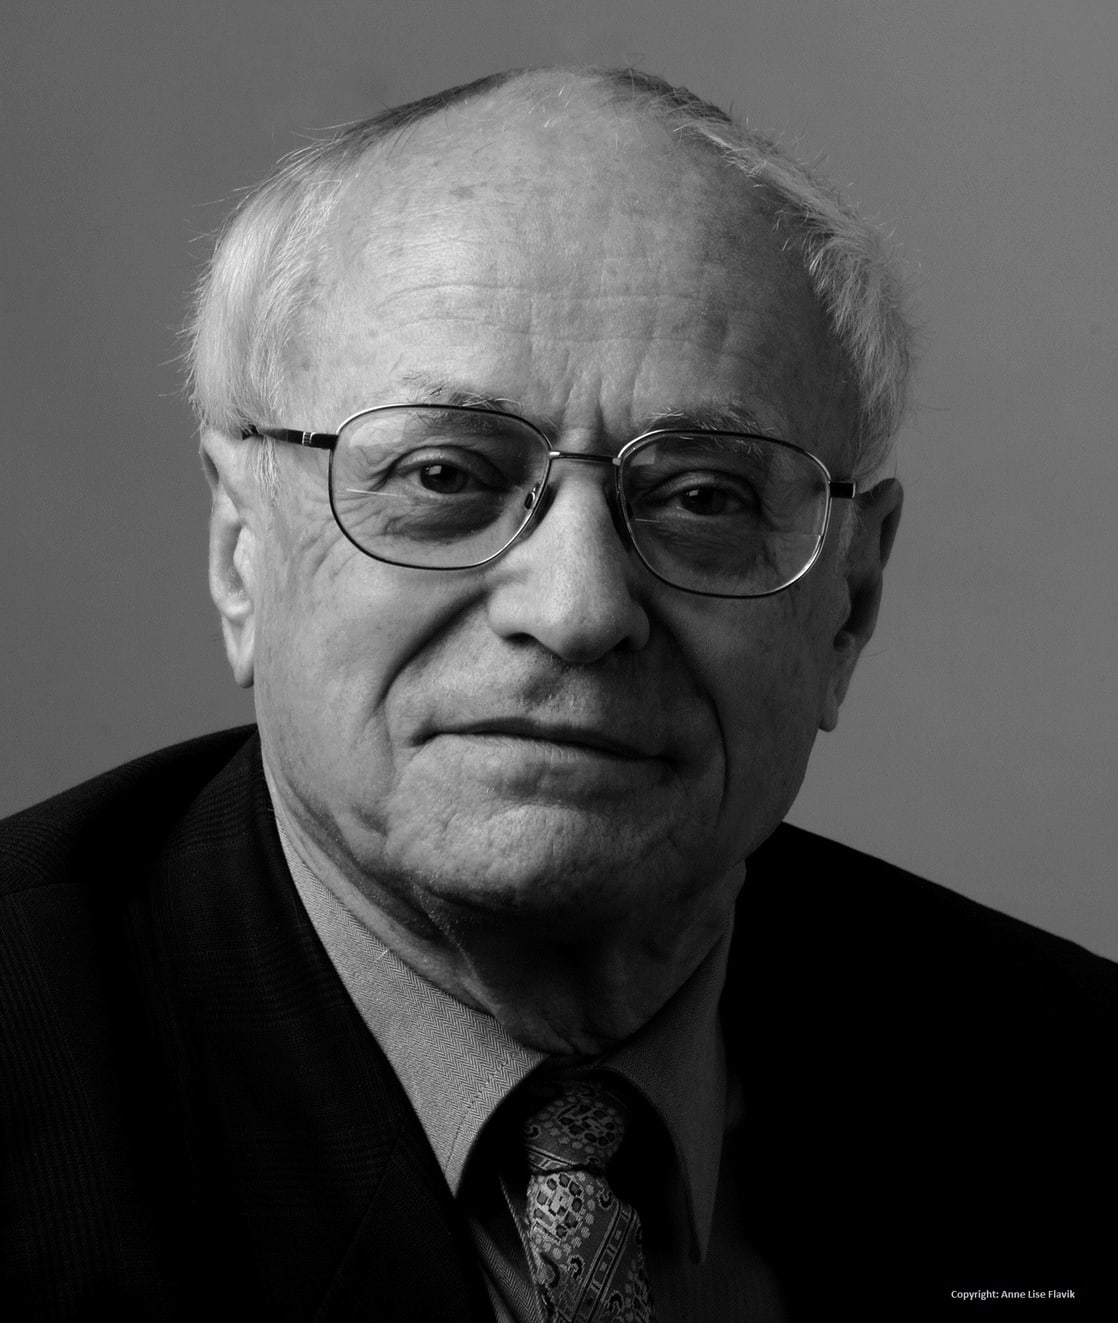
\includegraphics[scale=0.7]{images/serre}
\caption{Jean-Pierre Serre.}
\end{center}
\end{figure}
\fi
\begin{remark}
	A paper by Jean-Pierre Serre says, roughly, that analytic maps over projective manifolds tend to be algebraic whereas analytic things over affine manifolds are much more common than algebraic things.\footnote{``G\'eom\'etrie alg\'ebrique et g\'eom\'etrie analytique'' (GAGA), 1956.}
\end{remark}


\begin{example}[An automorphism of the affine plane]\label{}
Consider the endomorphism $\mathbf{A}^2\longrightarrow \mathbf{A}^2$ given by
\begin{align*}
	(z_1,z_2)\longmapsto  (z_1,z_1z_2).
\end{align*}
The image is not open, closed, or even locally closed. A theorem of Chevalley says that it must be a constructible set.\footnote{See EGA IV Th\'eor\`eme 1.8.4 (?).} For projective manifolds, the image of a closed set is closed.
\end{example}

\subsection{The Ax--Grothendieck theorem.}
\begin{remark}
	[First-order logic]\index{first-order logic} In first-order logic, one uses the usual logical connectives $\land$, $\lor$, $\lnot$, $\implies$, etc. to make statements. Also, one can use the operations of the field or model in question. One may also quantify over all elements in the model $X$ (with ``for all $x\in X$, . . .'' or ``there exists $x\in X$, . . .'').

	Here's an attempt at saying, ``$\Omega$ is algebraically closed'':
	\begin{quote}
		\small 
		For all polynomials $a_nX^n + \cdots + a_1X + a_0\in \Omega[X]$, there is a root.
	\end{quote}
	This is not allowed in first-order logic: One cannot say ``For all polynomials . . . .'' Here's the closest one can get:
	\begin{quote}
		\small 
		For all polynomials of degree $n$, there is a root.
	\end{quote}
	This is allowed because it is a statement on $n$ coefficients in $\Omega$. To say that $\Omega$ is algebraically closed takes infinitely many statements in first-order logic. One cannot quantify over all integers.
\end{remark}
\begin{definition}[ ]\label{}
A theory is \defn{complete}\index{complete theory} if every statement in it is provable or disprovable.
\end{definition}

\begin{proposition}[ ]\label{}
The theory of algebraically closed fields of a given characteristic is complete.
\end{proposition}

\begin{proof}
There is a unique algebraically closed field of a given characteristic and cardinality $\mathfrak{c}$.
\end{proof}

\begin{remark}
	This means that anything true for all algebraically closed fields of large characteristic is true for algebraically closed fields of characteristic $0$. One cannot say that $\Omega$ is of characteristic $0$ with one statement in first-order logic. One needs a countably infinite number of statements: For every prime number $p$, the statement
	\begin{quote}
		\small 
		For all $\omega\in \Omega$, $p\omega\ne 0$.
	\end{quote}
	must be true. Suppose you have proved something for algebraically closed fields of characteristic $0$. This proof uses only a finite number of axioms; that is, this proof can only eliminate a finite number of characteristics. Therefore, true for algebraically closed and characteristic $0$ implies true for algebraically closed and large characteristic.

	The converse is clearly true.
\end{remark}

\begin{theorem}[Ax--Grothendieck]\label{}\index{Ax--Grothendieck theorem}
Let $V$ be a variety over an algebraically closed field $K$. Let $f:V\longrightarrow V$ be a regular map. If $f$ is injective, then $f$ is surjective.
\end{theorem}

\begin{example}[$K$ must be algebraically closed]\label{}
Consider $K= \mathbf{Q}$ and $f:\mathbf{A}^1\longrightarrow \mathbf{A}^1$ given by $f(z)=z^ 3$. This is injective but not surjective.
\end{example}

\begin{example}[The converse is false]\label{}
Let $K=\mathbf{C}$ and $f(z)=z^2$. This is surjective but not injective.
\end{example}

\begin{proof}
This is trivial if $K$ is finite. Also, this is true over any algebraic extension of a finite field: The coefficients of all equations defining a variety and those of a point lie in some finite field. It is true for algebraic closures of finite fields. Recall that a first-order statement is true for an algebraically closed field of characteristic zero if and only if it is true for algebraically closed fields of all sufficiently large characteristics. Also, if a first-order statement is true for one algebraically closed field of a given characteristic, it is true for all algebraically closed fields of that characteristic.
\end{proof}

\begin{remark}
	A well-known example of proving something for positive characteristics and extending it to characteristic $0$ is Mori's bend-and-break argument.
\end{remark}

\subsection{Rational maps.}
Suppose $Y$ is an affine variety. The coordinate ring $\mathscr{O}(Y)$ is an integral domain. Hence, one can construct the field of fractions $K(Y)$. Its elements are called \defn{rational functions}\index{rational function} on $Y$.

\begin{example}[ ]\label{}
Suppose that $Y=\mathbf{A}^2$. Then $\mathscr{O}(Y) = K[z_1,z_2]$ and $K(Y) =K(z_1,z_2)$. 
\end{example}

\begin{remark}
	Regular functions on affine varieties are analogous to holomorphic functions on Riemann surfaces; rational functions correspond to meromorphic functions.
\end{remark}

Now, suppose that $Y$ is a projective variety. The previous construction does not work because the ring of regular functions $\mathscr{O}(Y)$ is just $K$ (whose field of fractions is itself). Instead, a rational function is given by the following:
 \begin{enumerate}
	\item A dense affine open set $U$;
	\item A rational function $f$ on $U$.
\end{enumerate}
One identifies $(f_1,U_1)$ and $(f_2,U_2)$ if $f_1=f_2$ on a dense open set containing $U_1$ and $U_2$. One gets the rational functions by taking a direct limit over dense open affine sets $U$ of the ring of regular functions on $U$. Therefore, the rational functions $K(Y)$ form a field.

\begin{remark}
	We are supposing that $Y$ is irreducible. One can define rational functions on a reducible algebraic set, but, then, the rational functions do not form a field.
\end{remark}

Suppose $X$ and $Y$ are varieties. A \defn{rational map}\index{rational map} $X\longrightarrow Y$ is a regular map $U\longrightarrow Y$ where $U$ is dense and open in $X$. One identifies $(f_1,U_1)$ and $(f_2,U_2)$ if $f_1=f_2$ on an open set contained in $U_1\cap U_2$.

\begin{example}[ ]\label{}
Rational maps $X\longrightarrow \mathbf{A}^1$ are rational functions on $X$.
\end{example}

Rational maps do not form a category: Composition does not need to be defined! For example, the composition of $0:\mathbf{A}^1\longrightarrow \mathbf{A}^1$ and $f:\mathbf{A}^1\longrightarrow \mathbf{A}^1$ given by $z\longmapsto 1/z$ is not defined.

\begin{definition}[ ]\label{}
A rational map is \defn{dominant}\index{dominant rational map} if its image contains a dense open set.
\end{definition}

\begin{definition}
	Two varieties are \defn{birational}\index{birational equivalence} if they are equivalent in the category whose morphisms are dominant rational maps.
\end{definition}

\begin{remark}
	Birational equivalence is a cruder notion of equivalence than isomorphism.
\end{remark}

\begin{example}[ ]\label{}
Consider $\mathbf{A}^1$, $\mathbf{P}^1 $, the hyperbola $xy=1$ in $\mathbf{A}^2$, and the curve $x^3=y^2$. These varieties are birational. However, no two are isomorphic.

The varieties $\mathbf{P}^1\times \mathbf{P}^1$, $\mathbf{P}^2$, $\mathbf{A}^2$, and $\mathbf{A}^2-\{(0,0)\}$ are birational but not isomorphic.
\end{example}

\begin{remark}
	A variety that is birational to an affine space is called a \defn{rational variety}\index{rational variety}.
\end{remark}

\begin{problem}
	Find a non-rational variety.
\end{problem}

\begin{example}[ ]\label{}
Consider the curve $x^3+y^3=1$. Let us show that this is not birational to $\mathbf{A}^1$, and, more generally, that there is no dominant rational map from $\mathbf{A}^1$ onto it. 

Suppose that there is a dominant map from $\mathbf{A}^1$ to the curve (this is non-constant). This means we have rational functions $x$ and $y$ with $x(t)^3+y (t)^3 =1$. Clearing denominators, we have 
\begin{align*}
	f(t)^3+g (t)^3=h (t)^3
\end{align*}
where $f$, $g$, and $h$ are coprime polynomials. Factoring, we get
\begin{align*}
	(f(t)+g (t)) (f(t)+\omega g (t)) (f(t) + \omega^2g (t)) = h(t)^3.
\end{align*}
The ring $K[t]$ in which these polynomials live is a UFD. Therefore, each term must be a cube (up to units, but the units are constants which are cubes in an algebraically closed field). Write
\begin{align*}
	h_1 (t)^3 h_2(t)^3  h_3(t)^3 = h (t)^3.
\end{align*}
One can eliminate $f$ and $g$ from the three equations one gets and a linear relation between $h_1^3$, $h_2^3$, and $h_3^3$ emerges. Multiplying by constants, one gets another relation between polynomials in which the sum of the cubes of the first two is the cube of the third. 

This gives another equation of the form above. If $f$, $g$, and $h$ are not constants, then $h_1$, $h_2$, and $h_3$ have smaller degree. This is a contradiction.
\end{example}

\begin{remark}
	This works for exponent greater than or equal to $3$. The result is false for exponent $2$:
	\begin{align*}
		(1-t^2)^2 +  (2t^2)^2 =  (1+t^2)^2.
	\end{align*}
	This corresponds to the fact that $x^2+y^2=1$ is rational.
\end{remark}

\begin{remark}
	The variety $\mathbf{A}^1$ has genus $0$ and $x^3+y^3=1$ has genus $1$. We will prove that there is no non-constant map from something to something of higher genus.
\end{remark}

\subsection{Elliptic functions. Cubic curves.}
We shall use elliptic functions to show that some cubic curves in the plane are not birational to the affine line.

Recall that $\wp$ is elliptic, so $\wp(z+\lambda) = \wp(z)$ where $\lambda$ is a point in a lattice $\Lambda$. This doubly periodic function is not holomorphic; if such a function were holomorphic, it would be bounded in a fundamental domain, so bounded everywhere, hence constant by Liouville's theorem. 

How does one find elliptic functions? One way is to take a function $g$ and sum over the lattice:
\begin{align*}
	f(z) :=  \sum_{\lambda\in \Lambda}^{} g (z+\lambda).
\end{align*}
This does not converge for $g(z) = 1/z$. This converges well for $g(z) = 1/z^3$ and borderline for $g(z)=1/z^2$ (that is, it doesn't converge for $1/z^2$, but does for $1/z^{2+\varepsilon}$). Hence, we define
 \begin{align*}
	\wp(z) :=  \frac{1}{z^2} + \sum_{\lambda\ne 0}^{} \frac{1}{(z-\lambda)^2} - \frac{1}{\lambda^2}.
\end{align*}
One shows that this is doubly periodic by looking at its first derivative and noticing that it is doubly periodic and showing that the constant up to which $\wp$ is doubly periodic is $0$.

Let's look at its Laurent expansion at $z=0$:
\begin{align*}
	\wp(z) = z^{-2} + 0 z + *z^2 + \cdots.
\end{align*}
Now, its derivative:
\begin{align*}
	\wp'(z) = -2z^{-3} + *z +\cdots.
\end{align*}
Square the derivative:
\begin{align*}
	(\wp'(z)) ^2 = 4z^{-6} + *z^{-2} + *z^0 + \cdots.
\end{align*}
Further,
\begin{align*}
	4(\wp(z)) ^3 = 4z^{-6} + *z^{-2} + \cdots.
\end{align*}
Hence,
\begin{align*}
	(\wp'(z)) ^2 = 4(\wp(z)) ^3 +  *\wp(z) + * + z.
\end{align*}
The first part is doubly periodic with no poles, and the whole thing vanishes at $z=0$. Therefore, one has
\begin{align*}
	(\wp'(z)) ^2 = 4(\wp(z)) ^3 - g_2 \wp(z) -  g_3.
\end{align*}

Why are these called elliptic functions? The arc length of an ellipse is given by 
\begin{align*}
	\int_{0}^{t} \frac{ds}{\sqrt{4s^3 - as - b} }. 
\end{align*}
Such integrals are called elliptic integrals. Write
\begin{align*}
	\kappa(z) = -\int_{z}^{\infty} \frac{ds}{\sqrt{4s^3 -g_2s - g_3} }. 
\end{align*}
Extending $\kappa\inv$ to $\C$ gives $\wp$. The inverses of such functions are doubly periodic, so they were called elliptic functions.

Now, consider the curve $C:y^2 = 4x^3 - g_2x-g_3$. Put $y=\wp'(z)$ and $x=\wp(z)$, and one sees that $(x,y)$ is on this curve. Hence, one has a map $\mathbf{C}-\Lambda \longrightarrow C$ given by
\begin{align*}
	z\longmapsto (\wp'(z),\wp (z)).
\end{align*}
It's somewhat unfortunate that we have to ignore the lattice, so we can define a map $f$ from $\mathbf{C}$ to the projective curve given by $C$ where $f(\Lambda) = \{\infty\}$. 

We have a doubly periodic function on our hands, so we have a map from $\mathbf{C}/\Lambda$ to the projective curve.\footnote{This is a homeomorphism of topological spaces.} One notices that $\mathbf{C}/\Lambda$ is isomorphic to $S^1\times S^1$ as a topological space, so it is a torus.

Any rational curve is the same as $\mathbf{P}^1$ up to a finite number of points. The variety $\mathbf{P}^1$ is isomorphic to $S^2$ and the curve $C$ is isomorphic to the torus $S^1\times S^1$. Therefore, the two are not birational.

\begin{remark}
	We constructed a doubly periodic function by taking (essentially) $\sum_{}^{} 1/(z-\lambda)^2 $. One can also do this for (singly) periodic functions by taking the almost-convergent $\sum_{}^{} 1/(z-\lambda)$ and reordering by absolute value. This is $\pi\cot (\pi z)$. Taking the logarithmic derivative gives the product formula of $\sin$.
\end{remark}

\subsection{The rationality of cubic surfaces.}
We have seen that cubic curves such as $x^3+y^3+z^3=0$ in $\mathbf{P}^2$ are not rational. Now, look at a cubic suface $w^3+x^3+y^3+z^3= 0$ in $\mathbf{P}^3$. One might argue that setting $w=0$ gives a cubic curve in $\mathbf{P}^2$ that isn't rational, but this doesn't work. In fact, it is rational.

First, observe that it contains two not intersecting lines: $w+x=0, y+z=0$ and $w+y=0, x+\omega z=0$ where $\omega$ is a primitive cube root of unity. Pick one point on each line and connect them. The resulting line should intersect the surface at one other point (ignoring the possibility that it lies on the cubic surface). Therefore, we have sort of constructed a map from $\mathbf{P}^1\times \mathbf{P}^1$ to the cubic surface. This is a rational map that is not defined everywhere. One can conclude that this map is almost surjective. Does it have a rational inverse?

Suppose there is a point on the third line that another line that goes through the first two lines intersects. This is a contradiction, since we assumed that the first two lines were skew. Hence, it is injective and (with some work) has a rational inverse; this strongly suggests that it's birational to $ \mathbf{P}^1\times \mathbf{P}^1$, and it is. Therefore, if a cubic surface has two not intersecting lines, it is birational to $\mathbf{P}^1\times \mathbf{P}^1$. Let's look at a different argument.

Pick $6$ points in $\mathbf{P}^2$ in general position.\footnote{Here, ``general position'' means that no three points are on a line and not all are on a conic.} The space of cubic functions in three variables is $10$ dimensional. Consider the cubics that vanish on all $6$ points. This gives a $4$-dimensional space. Suppose this is spanned by $f_1$, $f_2$, $f_3$, and $f_4$.

Try to define a map $\mathbf{P}^2 \longrightarrow \mathbf{P}^3$ by 
\begin{align*}
	(x:y:z)\longmapsto  (f_1:f_2:f_3:f_4).
\end{align*}
However, this is not defined at the $6$ points. So this is a rational map, not a regular map. What is its image?

One guesses that it's a hypersurface, so assume so. What is the degree of this hypersurface? Pick a line in $\mathbf{P}^3$, say $f_1=f_2=0$. Both $f_1$ and $f_2$ are cubics, so \index{B\'ezout's theorem}B\'ezout's theorem says that they have $9$ points of intersection. Six of these are the points with which we started, which leaves $3$ points. Therefore, the hypersurface has degree $168$. (Just kidding: It has degree $3$).

The dimension of the space of cubics in $\mathbf{P}^3$ has dimension $20$. Therefore, the dimension of the space of cubic surfaces is $19$.\footnote{Think of each cubic surface as being a point in a parameter space. This parameter space is $\mathbf{P}^{19}$.}

The dimension of the parameter space of the six points is $6\cdot 2$. Further, $\dim (\Aut(\mathbf{P}^2))=8$ and $\dim(\Aut(\mathbf{P}^3)) =15$. The dimension of the space of cubic surfaces one gets by taking $6$ points in $\mathbf{P}^2$ is probably going to be $12+15-8=19$, which strongly suggests that one can get all nonsingular cubic surfaces from this construction. Dr. Borcherds:
\begin{quote}
	\small 
	[This argument's] got more holes in it than a piece of Swiss cheese.
\end{quote}

These kinds of arguments were typical of old school algebraic geometry. Proving this true claim takes a lot more work.

\begin{problem}
	How might one guess that there are $27$ lines on a cubic surface from this construction?
\end{problem}

Take $6$ points in $\mathbf{P}^2$ as before. The map above is indeterminate at these points, and there are lines on the cubic surface whose preimages are these points. That is, $6$ points give rise to $6$ lines on the cubic. One also gets $15$ lines in $\mathbf{P}^2$ through $2$ of the $6$ points whose images are lines on the cubic surface. Lastly, take a conic through five of the points. There are $6$ conics through $5$ points, and the image of each is a line on the cubic surface. Altogether, there are $27$ lines.

\subsection{Blowing up.}
\index{blow up} 
\begin{example}[ ]\label{}
Take the curve $y^2 = x^3 +x^2$. This has a singularity at $(0,0)$. Let $y=tx$. Then one has $t^2x^2 = x^3+x^2$, which factorizes as follows:
\begin{align*}
x^2(t^2 - (x+1)) =0.
\end{align*}
One gets $2$ curves in the $(x,t)$ plane: $t^2=x+1$ and $x=0$. We get rid of the singularity but pick up another curve. The curve $x=0$ is called the \defn{exceptional curve}\index{exceptional curve}. This is blowing up.
\end{example}


Suppose we want to blow up the $(x,y)$ plane $\mathbf{A}^2$ at $(0,0)$. We introduce two new variables $(X:Y)\in  \mathbf{P}^1$. Consider the points $((x,y),  (X:Y))$ in $\mathbf{A}^2\times \mathbf{P}^1$ such that 
\begin{align*}
	xY = Xy.
\end{align*}
If $(x,y)\ne (0,0)$, there is one point of $\mathbf{P}^1$ to which it corresponds. If $(x,y)= (0,0)$, any point in $\mathbf{P}^1$ satisfies this. This subset of $\mathbf{A}^2\times \mathbf{P}^1$ is called the \index{blow up}blow up of $\mathbf{A}^2$ at a point.\footnote{This is a \index{quasiprojective variety}quasiprojective variety.} One gets a map from the blow up to $\mathbf{A}^2$ given by
\begin{align*}
	((x,y), (X:Y)) \longmapsto (x,y).
\end{align*}
The preimage of a nonzero point in $\mathbf{A}^2$ is one point and that of $(0,0)$ is $\mathbf{P}^1$. The projective line $\mathbf{P}^1$ is covered by two affine lines: $X = 1$ and $Y=1$. If $X=1$, then we have the transformation $xY=y$, and, if $Y=1$, we have $x = Xy$.

This generalizes. Take $\mathbf{A}^n$ with coordinates $(x_1,\hdots, x_n)$ and $\mathbf{P}^{n-1}$ with coordinates $(X_1:\cdots : X_n)$. Consider the subvariety of $\mathbf{A}^n\times \mathbf{P}^{n-1}$ given by the relation $x_iX_j = x_jX_i$ for all $i$ and $j$. This maps onto $\mathbf{A}^n$. The inverse image of $(x_1,\hdots, x_n)$ is a point if it's not $(0,\hdots, 0)$ and $\mathbf{P}^{n-1}$ if it is. The space $\mathbf{P}^{n-1}$ is covered by affine subsets of the form $X_i=1$, so we get $X_j = x_j/x_i$. That is, the effect of blowing up on the subset $X_i$ is introducing new coordinates by dividing the original coordinates by $x_i$.

\begin{example}[Resolving a singularity]\label{ressing}
We haven't formally defined \index{singularity}singularities yet, but they're fairly straightforward to understand. The curve $y^2=x^3$ has a singular point at $(0,0)$. Let us blow up at $(0,0)$. Let $y=xt$, so 
\begin{align*}
	x^2(t^2-x)=0.
\end{align*}
In the $(x,t)$ plane, one has the exceptional curve $x=0$ and the curve $t^2=x$. These curves have no singular points.
\end{example}

\begin{example}[ ]\label{}
Consider the surface $x^2+y^2=z^2$.\footnote{This is a cone.} There is a singularity at $(0,0,0)$. Let us blow up at $(0,0,0)$. Choose to divide by $z$, so $y=zs$ and $x=zt$. One gets
\begin{align*}
	z^2(t^2+s^2-1)=0.
\end{align*}
In the $(z,s,t)$ plane, the surface in question transforms into a cylinder given by $t^2+s^2-1$ and the exceptional plane $z=0$. The singularity has been resolved.
\end{example}

\begin{example}[ ]\label{}
Consider $y^8=z^5$. Blow this up once: If one divides $y$ by $z$, let $z=yt$. Then
\begin{align*}
	y^5(t^5-y^3)=0.
\end{align*}
The curve $y=0$ is exceptional, and $t^5-y^3$ still has a singularity, so blow it up again. Let $y= ts$. Therefore,
\begin{align*}
	t^3(s^3-t^2)=0.
\end{align*}
The curve $t=0$ is exceptional, and one blows up $s^3=t^2 $ by letting $t=su$, which means that $s=0$ and $s=u^2$ (see \cref{ressing}). Finally, the singularity has been resolved. 
\end{example}

\begin{example}[Pinch point\index{pinch point}]\label{ppoint}
Consider $xy^2=z^2$.\footnote{This is the \defn{Whitney umbrella}\index{Whitney umbrella}.} The points on the $x$ axis are the only singular points. The point $(0,0,0)$ seems to be worse off than the rest of them, so we blow it up. Take the variety $\mathbf{A}^3 \times \mathbf{P}^2$ with coordinates $((x,y,z),  (X:Y:Z))$. Choose one of the projective coordinates to be $0$ such that one of the affine pieces covers it. Dividing by $x$, we let $y=xY$ and $z=xZ$. Then, we get
\begin{align*}
	x^2(xY^2-Z^2)=0.
\end{align*}
Hence, we have transformed the singularity into an exceptional curve and another singularity. Notice that the new singularity is the same as the one with which we started. Oh no. Well, we can blow up a line, not just a point.

Take coordinates $(x,y,z)$, and, instead of taking $\mathbf{P}^2$, take $\mathbf{P}^1$ with coordinates $(s:t)$. Assert $yt=zs$. We have $xy^2=z^2$, so if we blow up along this line, we should choose $s=1$ or $t=1$. Choose $s=1$. Then $yt=z$. Thus, $y^2=0$ or $x=t^2$.
\end{example}

\begin{warn}
	One needs to define ``worst singularity'' in a very precise manner, as corroborated in \cref{ppoint}. 
\end{warn}

\subsection{Blowing up continued.}
\begin{example}[Blowing up a point of $\R^2$]\label{}
Blow up $(0,0)\in  \mathbf{R}^2$. Consider the coordinates $(x,y)$, and introduce new coordinates $(s:t) \in \mathbf{P}^1$. Take the set of points $((x,y), (s:t)) \in \mathbf{R}^2\times \mathbf{P}^1$ such that $xt=ys$. Every nonzero point in $\mathbf{R}^2$ corresponds to a unique point of the blow up and the zero point of $\mathbf{R}^2$ blows up to $\mathbf{P}^1_{\mathbf{R}}\isomto S^1$  (one can think of this having a point for every possible direction through the point). Hence, we have a map from the blow up to $\mathbf{P}^1_{\mathbf{R}}$ given by
\begin{align*}
	((x,y),  (s:t)) \longmapsto (s:t).
\end{align*}
The preimage of a point $(s:t) \in \mathbf{P}^1$ is a copy of $\mathbf{R}$. Let $E$ be the blow up. Then one has a map $E\longrightarrow S^1$ whose fibres are $\mathbf{R}$. One might guess that this might be a cylinder, but that's not right: The blow up is non-orientable\index{non-orientable surface}. Therefore, it is homeomorphic to an open M\"obius strip. 
\end{example}

\begin{example}[ ]\label{}\text{}
Let us construct a map 
\begin{align*}
	\mathbf{P}^1\times \mathbf{P}^1\longrightarrow \mathbf{P}^2.
\end{align*}
One might try with $((x_0:x_1),(y_0:y_1)) \longmapsto (x_0y_0:x_1y_0:x_0y_1)$. This is not defined if $x_0=y_0=0$, but we can make it so by blowing up $\mathbf{P}^1\times \mathbf{P}^1$ at $((0:1), (0:1) )$. Cover it with a copy of $\mathbf{A}^2$ with coordinates $(x_0,y_0)$ given by the points $x_1=1,y_1=1$. One blows up at $(0,0)$ and finds there is a map from this blown up plane to $\mathbf{P}^2$: Write $x_0=ty_0$, so $(x_0y_0:x_1y_0:x_0y_1)$ becomes $(ty_0^2:x_1y_0:ty_0y_1)$ or $(ty_0:x_1:ty_1)$. This is a good point of $\mathbf{P}^2$.

Therefore, one gets a regular map from the blow up of $\mathbf{P}^1\times \mathbf{P}^1$ to $\mathbf{P}^2$ from a rational map $\mathbf{P}^1\times \mathbf{P}^1\longrightarrow \mathbf{P}^2$.

\begin{remark}
	This regular map is not an isomorphism. The point $(0:0:1)\in  \mathbf{P}^2$ is the image of the line $y_0=0$ in $\mathbf{P}^1\times \mathbf{P}^1$ and $(0:1:0)\in \mathbf{P}^2$ is the image of the line $x_0=0$. This map is just the map one gets by blowing up these two points of $\mathbf{P}^2$. That is, the blow up of $\mathbf{P}^1\times \mathbf{P}^1$ at one point is the blow up of $\mathbf{P}^2$ at two points.
\end{remark}
\end{example}

The geometric meaning of blowing up a point is taking it to the projective space over its tangent space. We have seen that we can blow up a line, and, more generally, we can blow up a subvariety $X$; the geometric interpretation here is mapping a point in $X$ to the projective space over the normal space at that point. 

We can also blow up an ideal or a \index{quasicoherent sheaf}quasicoherent sheaf of graded algebras. One can construct a projective variety from a graded algebra. Suppose we have a graded algebra for every point in the variety and replace every point by the projective space of the corresponding graded algebra. That's a blow up. But how does one assign a graded algebra to every point of the variety? The nice way to do this is through a quasicoherent sheaf of graded algebras. This corresponds to the projective space of a graded algebra at each point.

There is one straightforward example to consider: Suppose the variety is a point. Then a quasicoherent sheaf of graded algebras is a graded algebra, say $K[z_0,\hdots,z_n]$. Blowing up a point along this sheaf is the usual construction of $\mathbf{P}^n$.

\begin{example}[ ]\label{introsing}\text{}
Consider the affine plane $\mathbf{A}^2$ with coordinate ring $K[z_1,z_2]$. Blowing up a point $(0,0)\in  \mathbf{A}^2$ corresponds to blowing up the ideal $(z_1,z_2)$. Suppose that $g_1,\hdots, g_n\in K[z_1,z_2]$ generate an ideal. Take the set of all pairs $((z_1,z_2), (g_1:\cdots:g_n))$ in $\mathbf{A}^2\times \mathbf{P}^{n-1}$ where $z_1$ and $z_2$ are not in the subvariety generated by the $g_i$s. Take the closure of the image of $\mathbf{A}^2- V$ in $\mathbf{A}^2\times \mathbf{P}^{n-1}$.

Take $I=(z_1^2,z_2^2)$. Then, take 
\begin{align*}
	(z_1,z_2)\longmapsto  ((z_1,z_2), (z_1^2:z_2^2)) \in \mathbf{A}^2\times \mathbf{P}^1.
\end{align*}
Write the elements in the image $((z_1,z_2),  (s:t))$. The projective line is covered by two copies of the affine line. Take $s=1$. Notice that $z_1^2t = z_2^2s$ so $z_1^2t=z_2^2$. This is the Whitney umbrella\index{Whitney umbrella}.
\end{example}

\begin{warn}
	One must be careful about blowing up. While Hironaka showed that blowing up always resolves singularities in characteristic $0$, if you blow up the wrong thing, you may introduce new singularities, as the end of \cref{introsing} demonstrated.
\end{warn}

\subsection{The Atiyah flop.}
\iffalse
\begin{figure}
\begin{center}
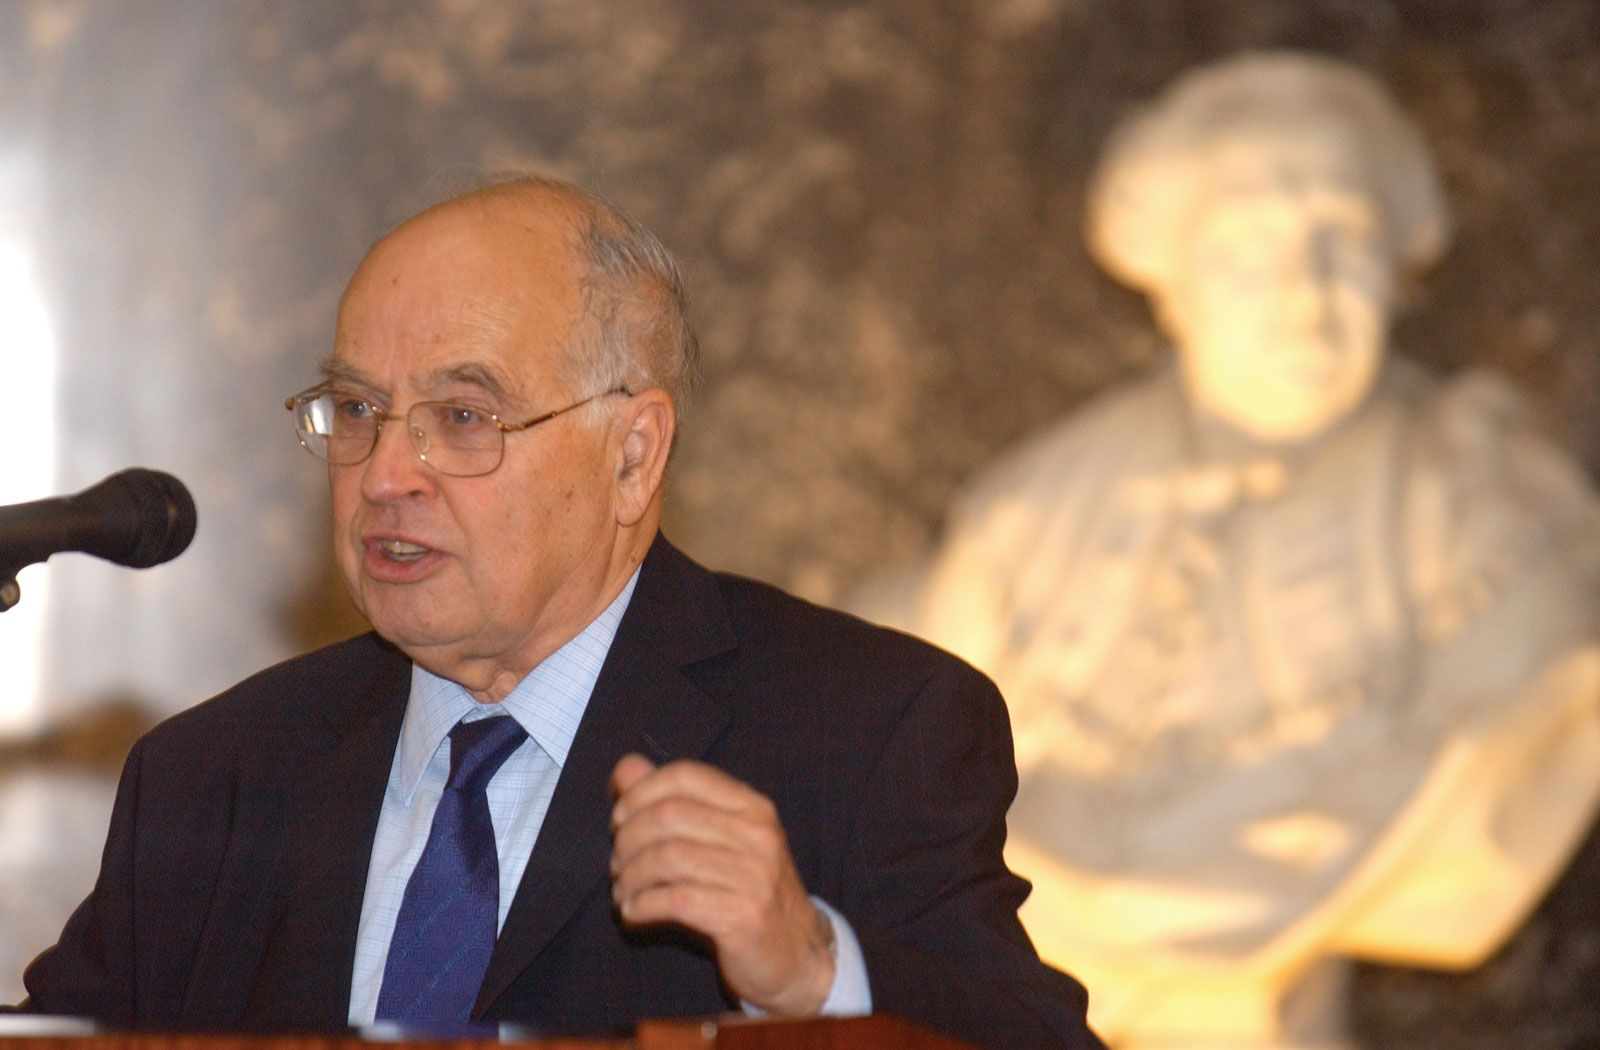
\includegraphics[scale=0.15]{images/atiyah}
\caption{Michael Atiyah.}
\end{center}
\end{figure}
\fi
Consider the hypersurface $xy=zt$ in $\mathbf{A}^4$. This looks like a cone over $\mathbf{P}^1\times \mathbf{P}^1$: One looks at the corresponding variety of points $(x:y:z:t)\in \mathbf{P}^3$ satisfying $xy=zt$. This is a quadric in projective space, which gives a product $\mathbf{P}^1\times \mathbf{P}^1$.\footnote{Cf. \cref{seg}.} In particular, this variety has a singularity at $(0,0,0,0)$ that is the singular point of the cone.

One resolves this singularity by blowing up at $(0,0,0,0)$. Consider points $((x,y,z,t),  (X:Y:Z:T)) \in \mathbf{A}^4\times \mathbf{P}^3$ satisfying $xy=zt$, $xY=Xy$, $xZ = Xz$, etc. Take the image of the nonzero points in $\mathbf{A}^4$ under
\[
	(x,y,z,t)\longmapsto  ((x,y,z,t),  (X:Y:Z:T))
	\]
	Taking the Zariski closure of the image, one has the equation $XY=ZT$. Every nonzero point of $\mathbf{A}^4$ corresponds to a unique point in the blow up $\mathbf{A}^4\times \mathbf{P}^3$ while $(0,0,0,0)$ corresponds to a copy of $\mathbf{P}^1\times \mathbf{P}^1$. This is not singular\iffalse, since, along $X=1$, it becomes $Y=ZT$ in the coordinates $(x,Y,Z,T)$\fi.

	One can also resolve this by blowing up to $\mathbf{P}^1$: Blow up along the line $y=t=0$. Consider the points $((x,y,z,t),  (X:Z)) \in \mathbf{A}^4\times \mathbf{P}^1$. Blowing up, we get the equations $xy=zt$ and $xZ=Xz$. However, taking the closure of the image of $\mathbf{A}^4$, we get the equation $tZ = Xy$, too. Say $X=1$. Then $y=tZ$, $z=xZ$, and $xy=tz$, which reduces to affine $3$-space. Hence, the blow up nonsingular. The point $(0,0,0,0)$ is blown up to $\mathbf{P}^1$.\footnote{One can also blow up along $x=z=0$, which results in a distinct resolution to $\mathbf{P}^1$.}

	The birational map from the first resolution to the second resolution is called the \defn{Atiyah flop}\index{Atiyah flop}.\footnote{This explanation from Wikipedia is slightly more clear: Let $Y$ be the zeros of $xy=zw$ in $\mathbf{A}^4$, and let $V$ be the blowup of $Y$ at the origin. The exceptional locus of this blowup is isomorphic to $\mathbf{P}^1\times \mathbf{P}^1$ and can be blown down to $\mathbf{P}^1$ in two different ways, giving varieties $X_1$ and $X_2$. The natural birational map from $X_1$ to $X_2$ is the Atiyah flop.}
	\begin{figure} 
		\begin{center}
			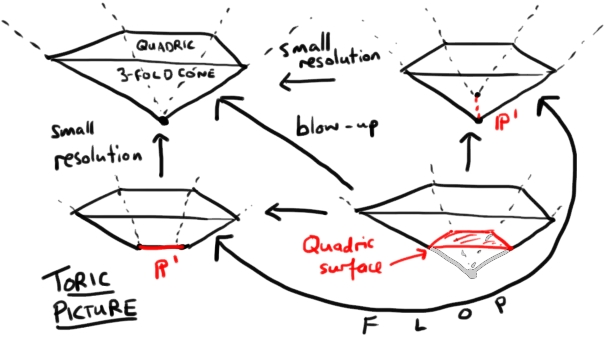
\includegraphics[scale=0.53]{images/flop_1}
			\caption{An illustration of a flop.}
		\end{center}
	\end{figure}

	\begin{figure}
		\begin{center}
			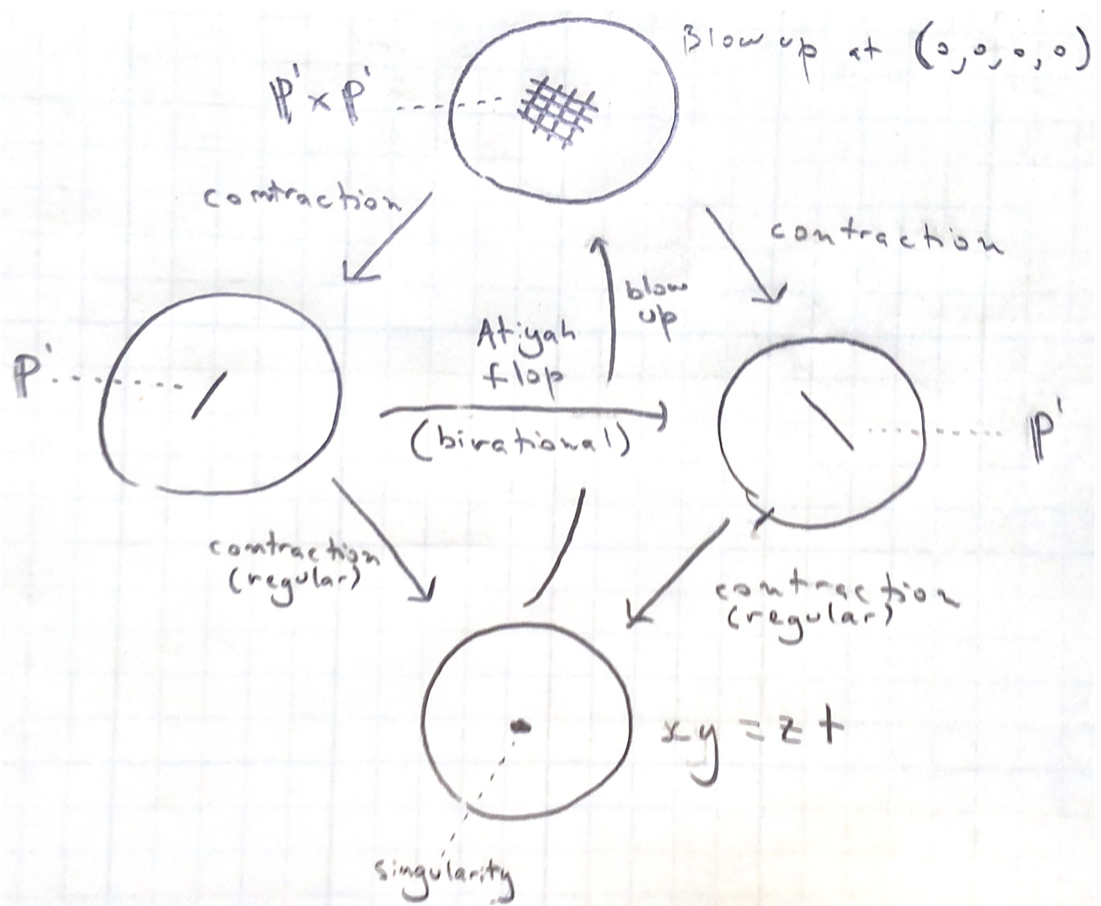
\includegraphics[scale=0.5]{images/atiyah_flop}
			\caption{An illustration of the Atiyah flop.}
		\end{center}
	\end{figure}

	This shows that there is no minimal way to resolve singularities in general. If one wants to find a minimal model---a ``smallest possible'' resolution of singularities---the best thing to do is to allow ``mild'' singularities in it.\footnote{More precisely, one allows for \index{terminal singularity}terminal singularities.}

\subsection{Singular points.}
Suppose that $p$ is a point of a variety $V$. The point $p$ is called \defn{singular}\index{singular point} if and only if the tangent space at $p$ has the wrong dimension.\footnote{That is, the dimension is greater than the dimension of $V$.}

Let $p=(0,\hdots, 0)\in  \mathbf{A}^n$ and let $V$ be the set of points at which an irreducible polynomial $f$ vanishes. Then, the \defn{tangent space}\index{tangent space} at $p$ is given by the roots of the linear part of $f$. For example, if this irreducible polynomial is $x-2y-3x^2+4xy =0$, then the tangent space is given by $x-2y=0$.

Let $f(x,y)=0$ be a plane curve. Saying that $(0,0)$ is singular is equivalent to saying that $f(0,0)=0$ and the linear terms vanish. If the linear terms vanish, then the tangent space is $\mathbf{A}^2$, which is the wrong dimension.

\begin{example}[ ]\label{}\text{}
For the curves $y^2 = x^3$ and $y^2 = x^3+x^2$, the tangent spaces at $(0,0)$ are $2$-dimensional.
\end{example}

If one has $f(z_1,\hdots, z_n) =0$, then saying that $(0,\hdots, 0)$ is singular is equivalent to saying that $f(0,\hdots,0)=0$ and the linear terms vanish: 
\begin{align*}
	\frac{\partial f}{\partial z_i}(0,\hdots, 0) =0.
\end{align*}

Suppose that $V\subseteq \mathbf{A}^n$ is the zero set of polynomials $f_1,\hdots$. Take $p=(0,\hdots, 0)$, so all of the $f_i$s vanish at $p$. The tangent space is the common roots of all linear parts of $f_1,\hdots$. The dimension of the tangent space is given by the rank of the Jacobian:
\begin{align*}
	\dim(\textrm{tangent space at $p$}) = n-\rank \frac{\partial f_i}{\partial x_j}.
\end{align*}
This is difficult to compute, in general, which is why we started with codimension-$1$ hypersurfaces. However, one sees that the subset of singular points is closed: The condition for a matrix having rank less than a fixed constant is a closed condition on the entries. Therefore, the condition for the tangent space having the wrong dimension is closed.

\begin{warn}
	For varieties, the set of singular points is closed, but this does not hold for schemes.
\end{warn}

\begin{proposition}[ ]\label{}\text{}
The nonsingular points of a variety are dense.
\end{proposition}

The nonsingular points comprise an open set, so one needs to show that the set of nonsingular points is nonempty. 

\begin{example}[ ]\label{}\text{}
Consider the variety $x^3+y^3=1$. Over $\mathbf{C}$, there are no singular points. However, over a field of characteristic $3$, all points are singular. What goes wrong: $x^3+y^3-1=(x+y-1)^3$ is not irreducible over $\mathbf{F}_{3}$.
\end{example}


First, we reduce to the case of hypersurfaces. The key is that every variety $V$ is birational to a hypersurface. Consider the function field $L$ of the variety $V$. Choose $z_1,\hdots, z_n$ such that $L$ is separable over $K(z_1,\hdots, z_n)$. Then, it is generated by $1$ element, so $L=K(z_1,\hdots, z_n,y)$ and $f(z_1,\hdots, z_n,y)=0$ for some $f$.

Consider the hypersurface $f(z_1,\hdots, z_n)=0$ where $f$ is irreducible. Also, suppose that the field $K$ over which we are working is algebraically closed. If all points are singular, then 
\begin{align*}
	\frac{\partial f}{\partial z_i} =0
\end{align*}
at all points of $V$. However, $\deg \partial f/\partial x_i< \deg f$, and, since $f$ is irreducible, $f$ divides $\partial f/\partial z_i$, so $\partial f/\partial z_i =0$. This implies that $f=0$ in characteristic $0$ and that $f$ is a linear combination of $p$th powers of monomials in characteristic $p$. This implies that $f=g^p$, so $f=0$.\footnote{Since $K$ is algebraically closed.}

 \begin{remark}\label{convvv}
	At nonsingular points over $\mathbf{R}$ or $\mathbf{C}$, a variety $V$ looks like a smooth manifold locally.
\end{remark}

\begin{example}[The converse of \cref{convvv}]\label{}\text{}
Consider $y^2=x^3$ over $\mathbf{R}$. This is a topological manifold.
\end{example}

\subsection{The Zariski tangent space.}
We would like to determine a definition of ``tangent space'' that does not depend on how one embeds the variety $V$ into affine space.

 \begin{definition}[ ]\label{}\text{}
The \index{tangent space}tangent space at a point is the dual of the \index{cotangent space}cotangent space at that point.
\end{definition}

\begin{remark}
	From the perspective of differential geometry, this definition seems circular. However, while the tangent space is fundamental in differential geometry, the cotangent space is fundamental in algebraic geometry.
\end{remark}

One defines the cotangent space as $\mathfrak{m}/\mathfrak{m}^2$ where $\mathfrak{m}$ is the maximal ideal of the local ring\index{local ring} at the point---the ring of functions of the form $f/g$ where $g\ne 0$ there. Hence, one might think of $\mathfrak{m}$ as functions vanishing at the point. The local ring at a point does not depend on the embedding of the variety as desired, but is this definition the same as the earlier one?

Consider $p= (0,\hdots, 0)$ for simplicity and $V\subseteq \mathbf{A}^n$ with coordinates $(z_1,\hdots, z_n)$. The maximal ideal $\mathfrak{m}$ is generated by $z_1,\hdots,z_n$, so $V$ is the set of zeros of functions $f_1,\hdots, f_n$. Now, $\mathfrak{m}$ is $(z_1,\hdots, z_n)$ modulo $(f_1,\hdots, f_n)$ and all monomials of degree greater than or equal to $2$. This is the vector space spanned by $z_1,\hdots, z_n$ modulo the linear parts of the $f_i$s. This is the dual of the tangent space. Therefore, the new definition is compatible with the old one.

\begin{remark}
	This definition works for any local ring $R$: The quotient $\mathfrak{m}/\mathfrak{m}^2$ is a vector space over $R/\mathfrak{m}$. The space $\mathfrak{m}/\mathfrak{m}^2$ is called the \defn{Zariski cotangent space}\index{Zariski cotangent space} of the local ring. The \defn{Zariski tangent space}\index{Zariski tangent space}, naturally, is the dual of this.
\end{remark}
\iffalse
\begin{figure}
\begin{center}
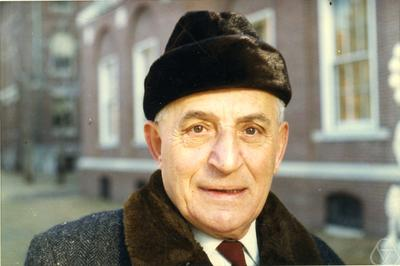
\includegraphics[scale=0.8]{images/zariski}
\caption{Oscar Zariski.}
\end{center}
\end{figure}
\fi

Let $R$ be a local ring. The quotient $\mathfrak{m}/\mathfrak{m}^2$ is an $R/\mathfrak{m}$--vector space whose dual $(\mathfrak{m}/\mathfrak{m}^2) ^*$ can be seen as ring homomorphisms 
\begin{align*}
	R\longrightarrow K[\varepsilon]/(\varepsilon^2).
\end{align*}
The target here is a two-dimensional vector space with a basis $\{1,\varepsilon\}$ and $\varepsilon^2=0$. This takes $\mathfrak{m}^2$ to $(0)$ and $\mathfrak{m}$ to multiples of $\varepsilon$. A ring $K[z_1,\hdots, z_n]/I$ often corresponds to a variety or algebraic set. However, this only works if $I$ is reduced (has no nilpotents), and $\varepsilon$ is nilpotent. 

This ring corresponds to the scheme $\Spec K[\varepsilon]/(\varepsilon^2)$. The only prime ideal of $K[\varepsilon]/(\varepsilon^2)$ is $(\varepsilon^2)$, so one might say its spectrum looks like a point; however, it is better thought of as a point with a tangent vector corresponding to the point $\varepsilon$.

Consider vector fields on a smooth manifold $V$ over $\mathbf{R}$. Look at the ring of smooth functions $C(V)$. The space of vector fields is a $C(V)$-module. Define the module $W$ of cotangent vector fields to be the dual of the module of vector fields. Recall, from differential geometry, that there is a map
\begin{align*}
	d:C(V) \longrightarrow W
\end{align*}
where $f$ maps to its $1$-form. Note that $d$ is not linear and satisfies Leibniz's rule. 

Instead of considering $C(V)$, one might consider $R=K[z_1,\hdots, z_n]/I$.\footnote{See \url{https://en.wikipedia.org/wiki/Kähler_differential}.} One wants to find a map $d$ from $R$ to an $R$-module $W$ that one thinks of as the module of cotangent vectors.

Note that $W$ is generated over $R$ by elements $dr$ for $r\in R$. One asserts that $dr=0$ for $r\in K$ and that Leibniz's rule holds. Define $W$ to be the module with these generators and relations.

\begin{example}[ ]\label{}\text{}
Take $R=K[z_1,\hdots, z_n]$. Then, $W$ is the free module on $dz_1,\hdots, dz_n$. One defines the module of tangent vector fields by $\Hom_{R}(W, R)$.
\end{example}

\begin{remark}
	The module $W$ is free only when the cotangent bundle is a sum of trivial bundles. Otherwise, $W$ is quite difficult to compute.
\end{remark}

Consider the homomorphism $R\tensor R\longrightarrow R$.\footnote{For now, $\tensor\equiv\tensor_K$.} Let $\mathfrak{h}$ be the kernel of this homomorphism. Write $W = \mathfrak{h}/\mathfrak{h}^2$.\footnote{Note that $\mathfrak{h}$ is an ideal of $R\tensor R$.} Define 
\begin{align*}
	d :R\longrightarrow W
\end{align*}
by $dr = 1\tensor r - r\tensor 1$. The set $W$ is an $R$-module: $R$ acts by multiplication on the left $R$ in $R\tensor R$. Leibniz's rule holds. However, one needs to check the universal property.

That is, suppose there is an $R$-module $M$ with a map $d:R\longrightarrow M$ satisfying Leibniz's rule and a map from $R$ to $W$. One wants to show that there is a unique map such that
\begin{center}
	\begin{tikzcd}
		R \ar[r, "d"] \ar[dr, swap, "d"]&M\\&W\ar[u,dashed]
	\end{tikzcd}
\end{center}
commutes. One has $\mathfrak{h}\subseteq R\tensor R\longrightarrow R$, a map $R\longrightarrow \mathfrak{h}$, and a map $d:R\longrightarrow M$. One can define $f:R\tensor R\longrightarrow M$ by $a\tensor b \longmapsto a(db)$. This gives a map $f:\mathfrak{h}\longrightarrow M$. However, we want a map from $\mathfrak{h}/\mathfrak{h}^2$ to $M$, so we check that $f$ is $0$ on $\mathfrak{h}^2$.

Pick $\sum_{i}^{} s_i\tensor t_i\in \mathfrak{h}$ and $\sum_{j}^{} u_j\tensor v_j\in \mathfrak{h}$. So $\sum_{i}^{} s_it_i=0$ and $\sum_{j}^{} u_jv_j=0$. Now
\begin{align*}
	f \left( \left( \sum_{i}^{} s_i\tensor t_i \right)\tensor \left( \sum_{j}^{} u_j\tensor v_j \right)  \right)&= \sum_{i,\,j}^{} s_iu_j\, d(t_iv_j) \\
														   &= \left( \sum_{i}^{} s_i\, dt_i \right) \underbrace{\left( \sum_{j}^{} u_jv_j \right)}_{0} \\ &\phantom{=}\ + \underbrace{\left( \sum_{i}^{} s_it_i \right)}_{0} \left( \sum_{j}^{} u_j\, dv_j \right) \\
														   &=0
\end{align*}
as desired.

From here, it is straightforward to show that $W$ is the universal module with a map $R\longrightarrow W$ satisfying Leibniz's rule.


\begin{remark}
	A local ring is \defn{regular}\index{regular local ring} if and only if the dimension of the Zariski tangent space is the dimension of the local ring. A variety is nonsingular at a point if its local ring is regular.
\end{remark}

\subsection{DV singularities.}
Other names for a \index{DV singularity}DV singularity include \index{simple surface singularity}``simple surface singularity,'' \index{Kleinian singularity}``Kleinian singularity'', \index{rational double point}``rational double point,'' and \index{canonical singularity}``canonical singularity'' in dimension $2$.

Take a finite group $G$ acting on $\mathbf{C}^2$. Consider $\mathbf{C}^2/G$. For reasonable groups $G$, this gives a variety that has a singular point at the origin. Recall that this quotient is the ring of invariants of the coordinate ring of $\C$ under $G$: $K[z_1,z_2]^G$. 

Suppose that $G=\Zmod n$ is generated by $\sigma$. Suppose further that $\sigma z_1 = \zeta z_1$ and $\sigma z_2 =\zeta^{-1}z_2$ where $\zeta$ is a primitive $n$th root of unity. Invariants under this action are given by $X =z_1^n$, $Y=z_2^n$, and $Z=z_1z_2$. Hence, one has
\begin{align*}
	K[z_1,z_2]^G = K[X,Y,Z] / (Z^n- XY).
\end{align*}

DV singularities are classified as follows:
\begin{center}
	\begin{tabular}{lcr}
		Name		& Notation	& Singularity\\
		\midrule
		Cyclic		& $\operatorname{A}_n$	& $x^2+y^2+z^{n+1}=0$\\
		Dihedral		& $\operatorname{D}_n$& $x^2+zy^2+z^{n-1}=0$\\
		Tetrahedral	& $\operatorname{E}_6$	& $x^2+y^3+z^4=0$\\
		Octahedral	& $\operatorname{E}_7$	& $x^2+y^3+yz^3=0$\\
		Icosahedral	& $\operatorname{E}_8$	& $x^2+y^3+z^5=0$
	\end{tabular}
\end{center}

The binary icosahedral group of order $120$---not the icosahedral group of order $60$---acts on $\mathbf{C}^2$ and gives the icosahedral singularity. 
\begin{remark}
	For the remainder of this section, we work in characteristic $0$ and the only singular point is $(0,0,0)$.
\end{remark}
\begin{example}[Resolving the icosahedral singularity]\label{}\text{}
The idea is to blow up the singular point until we don't get a singular point back. Consider the variety $x^2+y^3+z^5=0$. Let us introduce coordinates in $\mathbf{P}^2$ given by $(x_1:y_1:z_1)$. Assert $xy_1=x_1y$, $xz_1=x_1z$, and $yz_1=y_1z$. The projective plane $\mathbf{P}^2$ is covered by $3$ copies of $\mathbf{A}^2$ given by $x_1=1$, $y_1=1$, and $z_1=1$. Making $x_1=1$ means we have $y=y_1z$ and $z=xz_1$. This gives 
\begin{align*}
	x^2+x^3y_1^3+x^5z_1^5=0.
\end{align*}
One checks that $1+xy_1^3 + x^3z_1^5=0$ is nonsingular. For $y_1=1$, one gets something similar:
\begin{align*}
	x_1^2y^2 + y^3 +y^5z_1^5=0.
\end{align*}
Again, this is nonsingular. Now, suppose $z_1=1$. Then $x=x_1z$ and $y=y_1z$, so
\begin{align*}
	x_1^2z^2 + y_1^3z^3 + z^5 =0.
\end{align*}
Checking derivatives, one sees that $x_1^2 + y_1^3z+z^3=0$ is singular at $x_1=y_1=z=0$.

Now, let us blow up $x_1^2+y_1^3z+z^3=0$. Introduce coordinates in $\mathbf{P}^2$ given by $(x_2:y_2:z_2)$. Again, one covers $\mathbf{P}^2$ with $3$ copies of $\mathbf{A}^2$ corresponding to $x_2=1$, $y_2=1$, and $z_2=1$. One sees that there are no singularities corresponding to $x_2=1$ or $z_2=1$.For $y_2=1$, one makes the substitutions $z=y_1z_2$ and $x_1=x_2y_1$ to get
\begin{align*}
	x_2^2y_1^2 + y_1^4z_2+y_1^3z_2^3=0.
\end{align*}
One finds that $x_2^2+y_1^2z_2+z_1z_2^3=0$ has one singularity at $(0,0,0)$.\footnote{Determining the ``complexity'' of a singularity is challenging: While this singularity looks ``as bad'' as the last one, it's ``simpler'' by some mysterious invariant.}

Blow up $x_2^2+y_1^2z_2+z_1z_2^3=0$. Introduce coordinates in $\mathbf{P}^2$ given by $(x_3:y_3:z_3)$. Cover $\mathbf{P}^2$ by $3$ copies of $\mathbf{A}^2$ given by $x_3=1$, $y_3=1$, and $z_3=1$. One has no singularities for $x_3=1$. For $y_3=1$, one gets the equation 
\begin{align*}
	x_3^2+y_1z_3+y_1^2z_3^3 =0
\end{align*}
and finds that the only singularity is at $x_3=y_1=z_3=0$. For $z_3=1$, one gets
\begin{align*}
	x_3^2+y_3^2z_2+y_3z_2^2 =0
\end{align*}
and sees that there is a singularity at $x_3=y_3=z_2=0$.

Let us look at the singularity of $x_3^2+y_1z_3+y_1^2z_3^3 =0 $. Introduce coordinates of $\mathbf{P}^2$ given by $(x_4:y_4:z_4)$ and cover $\mathbf{P}^2$ by $x_4=1$, $y_4=1$, and $z_4=1$. Each of the corresponding varieties have no singularities.

Now, let us consider the singularity of $x_3^2+y_3^2z_2+y_3z_2^2 =0$. Introduce coordinates $(x_5:y_5:z_5)$ of $\mathbf{P}^2$. The variety given by $x_5=1$ has no singularities. However, that given by $y_5=1$ has $2$ singularities: $x_5=0$, $y_3=0$, $z_5=0,-1$. That given by $z_5=1$ has $2$ singularities, too: $x_5=0$, $z_2=0$, $y_5=0,-1$. Two of these singularities are really the same, so one gets three singularities. 
When one blows up these three varieties, the singularities all resolve.
\end{example} 

After $8$ blowups, we ended up with something nonsingular. Each blowup gives an exceptional curve that looks like $\mathbf{P}^1$. If one considers how they intersect and takes the dual, one gets the $\E_8$ Dynkin diagram. 

\begin{figure}
	\begin{center}
		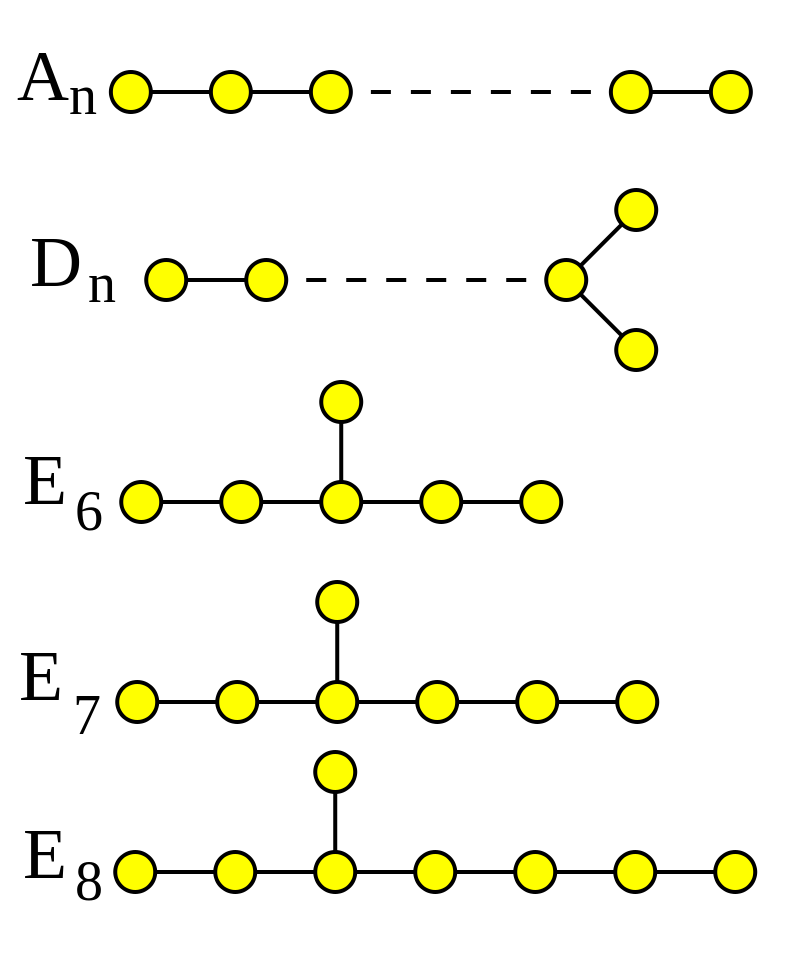
\includegraphics[scale=0.225]{images/simply_laced}
		\caption{Simply-laced Dynkin diagrams.}
	\end{center}
\end{figure}

\subsection{Examples of resolutions.}
\begin{example}[ ]\label{}\text{}
Consider $x^4+y^4=z^2$.\footnote{Fermat showed that this equation has no integer solutions, demonstrating Fermat's last theorem for $n=4$.} Differentiating, one gets $4x^3=0$, $4y^3=0$, and $2z=0$. Therefore, the only singularity here is at $(0,0,0)$. Let us blow up the point $(0,0,0)$. Hence, we work in $\mathbf{A}^3\times \mathbf{P}^2$, introducing new coordinates $(X:Y:Z)$ in $\mathbf{P}^2$. We assert $xY=Xy$, $xZ=Xz$, and $yZ=Yz$. Cover $\mathbf{P}^2$ by three copies of $\mathbf{A}^2$ corresponding to $Z=1$, $Y=1$, and $X=1$. For the first case, one gets 
\begin{align*}
	z^2X^4+z^2Y^4=1.
\end{align*}
This is nonsingular. For the second case, one gets
\begin{align*}
	y^2X^4+y^2=Z^2.
\end{align*}
This has singularities whenever $y=Z=0$. A similar thing happens with $X=1$.\footnote{There is a projective line of singular points.}

\begin{remark}
	A singularity's ``complexity'' has more to do with its codimension than its dimension.
\end{remark}

Let us blow up $y^2X^4+y^2=Z^2$ along $y=Z=0$. Introduce coordinates $(s:t)$ where $sZ=ty$. With $s=1$, one gets 
\begin{align*}
	X^4 + 1=t^2,
\end{align*}
which is nonsingular. One also gets a nonsingular variety with $t=1$.
\end{example}


\begin{example}[Blowing up can make the singularity worse]\label{}\text{}
Consider $x^2-yz=0$. Instead of blowing up at the conical singularity $(0,0,0)$, blow up along $y=z=0$. Introduce coordinates $(Y:Z)$ of $\mathbf{P}^1$ where $yZ=Yz$. Take $Y=1$. Then, one gets
\begin{align*}
	x^2-y^2Z=0,
\end{align*}
which is the more complicated \index{Whitney umbrella}Whitney umbrella.
\end{example}

\begin{example}[ ]\label{}\text{}
The ring $\mathbf{Z}\!\left[\sqrt{-3}\right]$ does not have unique factorization:
\begin{align*}
	2\cdot 2 = (1+\sqrt{-3} ) (1-\sqrt{-3} ).
\end{align*}
Even though it is the coordinate ring of a scheme, pretend that $\mathbf{Z}\!\left[\sqrt{-3}\right]$ is the coordinate ring of a variety. This ring has a maximal ideal $(2,\sqrt{-3}-1 )$. If one, somehow, thinks of maximal ideals as points, one wants to show that the variety has a singular point at that maximal ideal. Let us look at the local ring $R=\Z_{(2)} \!\!\left[ \sqrt{-3}  \right] $ whose maximal ideal is $\mathfrak{m}=(2,\sqrt{-3}-1 )$. One sees that \begin{align*}
	R/\mathfrak{m} = \mathbf{F}_{2}.
\end{align*}
Further, $R/\mathfrak{m}^2$ has order $8$, so $\mathfrak{m}/\mathfrak{m}^2$ is a $2$-dimensional vector space over $R/\mathfrak{m}$.\footnote{Recall that $\mathfrak{m}/\mathfrak{m}^2$ is the \index{Zariski cotangent space}Zariski cotangent space at $\mathfrak{m}$.} The \index{Krull dimension}Krull dimension of $R$ is $1$ since the only prime ideals of $R$ are $(0)$ and its maximal ideals. One notices that this is smaller than the dimension of the cotangent space at $\mathfrak{m}$, so $\mathfrak{m}$ corresponds to a ``singular point.''

\begin{remark}
	The existence of a singular point is somehow related to unique factorization failing. However, there are some rings of algebraic integers with no singular points in which unique factorization fails. 
\end{remark}

Now, we will resolve this singularity. One can blow up, but we won't do that. To resolve a singularity in number theory, one might take the \defn{normalization}\index{normalization} (i.e. \defn{integral closure}\index{integral closure}) of the ring. The integral closure of $\Z\!\left[ \sqrt{-3}  \right] $ is
\begin{align*}
	\Z \!\left[ \frac{1+\sqrt{-3} }{2} \right] = \Z[\omega] .
\end{align*}
Since $\omega^2+\omega+1=0$, $\omega$ is an algebraic integer in the field of fractions of $\Z\!\left[ \sqrt{-3}  \right] $. This integral closure has unique factorization, and its points are nonsingular.
\end{example}

\begin{example}[Application of resolutions]\label{}\text{}
Recall that
\begin{align*}
	\Gamma(s) :=  \int_{0}^{\infty}\exp(-t)t^{s-1}  \, dt
\end{align*}
	converges for $\Re (s)>0$ and can be extended to a meromorphic function of $s$ by integrating by parts. Suppose that $f(z_1,\hdots,z_n)$ is a polynomial and $\varphi(z_1,\hdots, z_n)$ is a smooth function with compact support. Then,
	\begin{align*}
		\int_{0}^{\infty} \left\lvert f(z_1,\hdots, z_n) \right\rvert ^s\varphi(z_1,\hdots,z_n)  \, dz_1\cdots dz_n 
	\end{align*}
	will be a holomorphic function of $s$ for $s$ large enough. The question of whether one can continue this to all $s$ is, more or less, the situation of $\Gamma$.\footnote{Indeed, $\exp({-t})$ does not have compact support.} The problems here occur at the roots of $f$, which correspond to hypersurfaces with singularities.
	
	Atiyah suggested to use Hironaka's theorem to resolve the singularities of $\{f=0\}$. What one ends up with isn't really nonsingular, since blowing up introduces exceptional curves. These exceptional curves don't really matter, though, since they cross transversally. That is, when one blows up, one gets singularities $z_1\cdots z_k=0$ (one gets hyperplanes intersecting orthogonal to each other). Therefore, we reduce to 
	\begin{align*}
		\int_{}^{}  \left\lvert z_1\cdots z_n \right\rvert^s\varphi(z_1,\hdots,z_n)   \, dz_1\cdots dz_n =0.
	\end{align*}
	This splits into integrals of the form
	\begin{align*}
		\int\left\lvert z_i \right\rvert ^sf(z_i)\, dz_i=0,
	\end{align*}
	which one can do with integration by parts, just as one does with $\Gamma$. Hence, one can continue integrals of the form above. Bernstein came up with a much more simpler way of showing this using Bernstein (or Bernstein--Sato) polynomials.
\end{example}

\subsection{Completions.}
The completion of $R=K[z]$ is the formal power series ring $K[\![z]\!]$. \iffalse How does one get this, though? Take the ideal $I=(x)$. Then
\begin{align*}
	R/I&= k;\\
	R/I^2 &= \{a_0+a_1x:a_0,a_1\in k\};\\
	R/I^3 &= \{a_0+a_1x+a_2x^2:a_0,a_1,a_2\in k\};
\end{align*}
etc. An element One has a sequence
\[
\begin{tikzcd}
	\cdots \ar[r] &R/I^4\ar[r] &R/I^3\ar[r]&R/I^2 \ar[r] &R/I\\
		      &&\widehat{R}\ar[lu]\ar[u]\ar[ru]
\end{tikzcd}
\]
\fi Let's see how one gets this.

Consider the ideal $I=(z)$. Notice that there is a natural surjective map $\varphi_n :R/I^{n+1} \longrightarrow R/I^{n}$. One says that the sequence
\[
\begin{tikzcd}
	\cdots\ar[r] &R/I^{n+1}\ar[r,"\varphi_n"]&R/I^n \ar[r] &\cdots\ar[r] &R/I^2 \ar[r,"\varphi_1"] &R/I 
\end{tikzcd}
\]
forms a \defn{projective system}\index{projective system} indexed by the natural numbers.
The completion of $R$ at $I$ is the \defn{projective limit}\index{projective limit} or \defn{inverse limit}\index{inverse limit} of the system $(R/I^n, \varphi_n)$; that is, an element of the completion
\begin{align*}
	\widehat{R}_I = \widehat{R} := \varprojlim (R/I^n, \varphi_n)
\end{align*}
is a sequence $z=(\hdots, z_n,\hdots,z_1)$ with $z_n\in R/I^n$ and $\varphi_n (z_n)=z_{n-1}$ if $n\ge 2$. This naturally extends to all rings $R$ and their ideals.

\begin{example}[ ]\label{}\text{}
Let $p$ be a prime number. Take $R=\mathbf{Z}$ and $\mathfrak{p}=(p)$. Then, the completion $\widehat{R}_{\mathfrak{p}} = \mathbf{Z}_p$ is the $p$-adic integers.
\end{example}

In algebraic geometry, one likes to consider the completion of a local ring $R$ at its maximal ideal $\mathfrak{m}$.

The natural map $R\longrightarrow \widehat{R}$ is injective if $R$ is Noetherian.

\begin{example}[The natural map does not need to be injective]\label{}\text{}
\begin{enumerate}
	\item Let $R$ be all smooth functions on $\mathbf{R}$.\footnote{Note that $R$ isn't local.} Let $I=(z)$ be those functions that vanish at $0$. Then, the completion $\widehat{R}_I$ is given by power series. However, the natural map is not injective: Consider
		\begin{align*}
			f(z):=
			 \begin{cases}
				 e^{-1/z^2}&z\ne 0\\
				 0&z=0,
			\end{cases}
		\end{align*}
		which is in the kernel of the natural map.
	\item Let $R = K [\![z,z^{1/2},z^{1/4},\hdots]\!]$. Let $I=(z,z^{1/2},z^{1/4},\hdots)$.\footnote{$I=I^2$.} Then, $\widehat{R}_I = K$.
\end{enumerate}
\end{example}

An application of completions of rings is \defn{Hensel's lemma}\index{Hensel's lemma}. There are many different ``Hensel's lemmas'' that are context-dependent, but here's the main idea: Solutions in $R/\mathfrak{m}$ can be lifted to solutions in $\widehat{R}$ under some conditions.

\begin{example}[Factorizing polynomials]\label{}\text{}
Suppose $f(z)\equiv g_0(z) h_0(z)\pmod{\mathfrak{m}}$ where $g_0,h_0\in K[z]$ and $f\in R[z]$. Then this lifts to a factorization $f(z)=g (z)h (z)$ in $R[z]$ if $g_0$ and $h_0$ are coprime in $K[z]$.
\end{example}

\begin{esquisse}
	Suppose that $f\equiv gh\pmod{\mathfrak{m}^n}$. Try to find elements $a,b\in \mathfrak{m}^{n+1}/\mathfrak{m}^{n+2}$ such that $f\equiv (g+a) (h+b)\pmod { \mathfrak{m}^{n+1}}$. One needs to solve an equation $g_0b+h_0a = *$, which one can solve if $g_0$ and $h_0$ are coprime.\footnote{This relates to the fact that two coprime polynomials over a field generate the unit ideal.}
\end{esquisse}

\begin{example}[ ]\label{}\text{}
Consider the curve $y^2 = x^3+x^2$. Looking closely at its singularity, one wants to say that the curve is a union of lines that intersect there. However, one struggles to see this looking at the local ring. If the local ring allowed for this, then it would have zero divisors, and it doesn't. The local ring isn't ``aware'' that the curve seems to split into two components near the origin. However, the completion is. 

Let $R$ be the local ring at $(0,0)$. Let $\widehat{R} = K [\![x,y]\!]/(y^2-x^3-x^2)$. Notice that $y^2-x^3-x^2\equiv (y-x) (y+x)\pmod {I^3}$. One lifts this to a product of power series $(y-x+\cdots) (y+x+\cdots)$. This corresponds to the components.
\end{example}

\begin{remark}
	One says that the varieties $y^2=x^3+x^2$ and $y^2=x^2$ are \defn{analytically isomorphic}\index{analytic isomorphism}; that is, the completions of their local rings are isomorphic.
\end{remark}

\begin{remark}
	The completion $\widehat{R}$ has zero divisors, though $R$ does not. There are examples of reduced rings whose completions are not reduced.
\end{remark}

\begin{remark}
	There is a variation on completion called \defn{Henselization}\index{Henselization} that is better behaved.
\end{remark}

One has the following maps:
\[
\begin{tikzcd}
	R\ar[r]&\widehat{R}\ar[r] &\cdots\ar[r] & R/\mathfrak{m}^2 \ar[r]& R/\mathfrak{m} = K.
\end{tikzcd}
\]
One can think of successive maps as focusing on a point in a finer neighbourhood.


\subsection{Resultants.}
This section will concern elimination theory. Andr\'e Weil's \ul{Foundations of Algebraic Geometry} has an infamous footnote:
\begin{quote}
	\small 
	The device that follows, which, it may be hoped, finally eliminates from algebraic geometry the last traces of elimination-theory, is borrowed from C. Chevalley's Princeton lectures.
\end{quote}
This is quite funny next to the following line from a poem by Shreeram Abhyankar:
\begin{quote}
	\small 
	Eliminate the eliminators of elimination theory!
\end{quote}

		Suppose you have two polynomials, say $x^3y^4 - 7x^2-xy^8$ and $3x^2y^5+4y^2+x^4y^7$. Now, suppose you want to eliminate $y$. The variable $x$ should satisfy a polynomial of degree $9\cdot 11$. Here's the general problem: Suppose
		\begin{align*}
			f(z)&=a_mz^m+\cdots +  a_1z+a_0;\\
			g(z)&=b_nz^n+\cdots +  b_1z+b_0.
		\end{align*}
What is the condition for $f$ and $g$ to have a common root? Temporarily suppose that $a_m\ne 0$ and $b_n\ne 0$. Then the condition is $f(z)p (z)=g (z)q (z)$ where $\deg p<n$ and $\deg q<m$. If $f$ and $g$ have a common root $\alpha$, one has
\begin{align*}
	p(z)&= \frac{g(z)}{z-\alpha};\\
	q(z)&= \frac{f(z)}{z-\alpha}.
\end{align*}
The equation $f(z)p (z)=g (z)q (z)$ gives homogeneous linear equations. The condition for homogeneous equations having a nontrivial solution is that some determinant vanishes. What one wants is the determinant of this matrix:
\begin{align*}
	\mat{a_m & \cdots & a_0 && &&\\ & a_m & \cdots & a_0& &&\\ &&&\ddots&&&\\&&&a_m & \cdots & a_0\\&&&&a_m & \cdots & a_0\\b_n & \cdots & b_0 && &&\\ & b_n & \cdots & b_0& &&\\ &&&\ddots&&&\\&&&b_n & \cdots & b_0\\&&&&b_n & \cdots & b_0 }.
\end{align*}
This $ (m+n)\times  (m+n)$ matrix is called the \defn{Sylvester matrix}\index{Sylvester matrix} and its determinant is called the \defn{resultant}\index{resultant} of $f$ and $g$.\footnote{The prefix ``ant'' indicates that the resultant is some invariant and that Sylvester probably named it.}

\begin{remark}\label{ifffffffffff}
	One can think of the case where the leading coefficient of a polynomial $f$ is $0$ as $f$ having a root at infinity: One expects that
	\begin{align*}
		f(z) = a_mz^m+\cdots+a_1z+a_0
	\end{align*}
	has $m$ roots, but it doesn't if $a_m=0$. One makes up for this by saying that $f$ has a root at infinity. One way to think about this is looking at the homogeneous polynomial
	\begin{align*}
		a_mz^my^0 + a_{m-1}z^{m-1}y^1+\cdots +a_1z^1y^{m-1} +a_0z^0y^m
	\end{align*}
	and considering a root to be a point $(z:y)\in  \mathbf{P}^1 = K\cup \{\infty\}$. The resultant is $0$ if and only if the homogenized polynomials have a common root in $\mathbf{P}^1$.
\end{remark}

\begin{example}[ ]\label{}\text{}
The polynomial $f(z)=az^2+bz+c$ has a double root if it and its derivative have a root in common.\footnote{This is true for all polynomials.} Let $g(z)=2az+b$ be the derivative of $f$. One sees that the resultant of $f$ and $g$ is
\begin{align*}
	\det\mat{a&b&c\\2a&b&0\\0&2a&b} = a(b^2-4ac).
\end{align*}
The factor $(b^2-4ac)$ is the well-known quadratic discriminant, and the factor $a$ corresponds to the case when the leading coefficient is $0$, as discussed in \cref{ifffffffffff}.  
\end{example}

\begin{example}[ ]\label{}\text{}
Let us see when $f(z)=z^3+bz+c$. has a double root. Write $g (z)= 3z^2 + b$ for the derivative of $f$. Then, the resultant of $f$ and $g$ is
\begin{align*}
	\det\mat{1&0&b&c&0\\0&1&0&b&c\\3&0&b&0&0\\0&3&0&b&0\\0&0&3&0&b}&= 4b^3+27c^2.
\end{align*}
Notice that the definition of the resultant allows for sign inaccuracy: The discriminant of a cubic is $-(4b^3+27c^2)$.
\end{example}

\subsection{Proper maps.}
Suppose $f$ and $g$ are homogeneous polynomials in $z_1$ and $z_2$ with coefficients in $K[y_1,\hdots, y_\ell]$. One might think of $f$ and $g$ as hypersurfaces $H_f$ and $H_g$ in $\mathbf{A}^\ell\times \mathbf{P}^1$. Consider the projection $\mathbf{A}^\ell\times \mathbf{P}^1\longrightarrow \mathbf{A}^\ell$. The condition that the resultants of $f$ and $g$ vanish (that is, the condition that $f$ and $g$ have a common root in $\mathbf{P}^1$) is that a point is in the image of $H_f\cap H_g\longrightarrow \mathbf{A}^\ell$. The image comprises the roots of the resultant (a polynomial in $K[y_1,\hdots,y_\ell]$). This is closed.

\begin{remark}
	It is a common mistake to think that the image of a closed set under a projection is closed.
\end{remark}

\begin{example}[ ]\label{}\text{}
The projection $\mathbf{A}^1\times \mathbf{A}^1 \longrightarrow \mathbf{A}^1$ is not closed: Consider $\{xy=1\}\longmapsto \mathbf{A}^1-\{0\}$.
\end{example}

\begin{exercise}\label{}\text{}
Show that the image of a polynomial under $\mathbf{R}^n\longrightarrow \mathbf{R}$ does not need to be closed.
\end{exercise}

We have seen that $\mathbf{P}^n_{\mathbf{R}}$ and $\mathbf{P}^n_{\mathbf{C}}$ are compact in the usual topology. Projective space over a field is compact in the Zariski topology, but even affine space over a field is compact in this setting.

\begin{problem}
	What is the correct analogue of compactness?
\end{problem}

First, let us digress. A map of topological spaces $X\longrightarrow Y$ is \defn{proper}\index{proper map} if and only if it is continuous and universally closed.\footnote{Recall that a map is \defn{universally proper}\index{universally proper morphism} if and only if $X\times W\longrightarrow Y\times W$ is closed for all $W$.} Notice that this is equivalent to saying that $X\longrightarrow Y$ is continuous and closed and has compact fibres.

Maps of Hausdorff spaces are proper if and only if they are continuous and the preimage of a compact set is compact.

A map of varieties $X\longrightarrow Y$ is called \defn{proper}\index{proper map} if it is universally closed for the Zariski topology on the product $X\times Y$. 

Now, we have somewhat of an analogue: Saying that a map from $X$ to a point is proper is like saying that $X$ is compact. We would like to show that, if $X$ is a projective variety, then maps from $X$ to a point is proper. One can reduce this to showing that $\mathbf{P}^n\times \mathbf{A}^m\longrightarrow \mathbf{A}^m$ is closed.

First, let us show that $\mathbf{P}^1\times \mathbf{A}^m\longrightarrow \mathbf{A}^m$. Suppose that $S$ is closed in $\mathbf{P}^1\times \mathbf{A}^m$. Then $S$ is given by the roots of polynomials $f_1,\hdots, f_\ell$ in $x,y, z_1,\hdots,z_m$. Consider 
\begin{align*}
	&s_1f_1+s_2f_2+\cdots+s_\ell f_\ell;\\
	&t_1f_1+t_2f_2+\cdots+t_\ell f_\ell.
\end{align*}
These are homogeneous polynomials in $x$ and $y$ with coefficients that are polynomials in $s_1,\hdots,s_\ell,t_1,\hdots, t_\ell,z_1,\hdots, z_m$. The projection of $S$ to $\mathbf{A}^m$ is given by the points where these polynomials have a common root---given by roots of all of the coefficients of all of the monomials in $s_1,\hdots,s_\ell,t_1,\hdots, t_\ell$ of the resultant. One can show that this implies that a map from $\mathbf{P}^1$ to a point is proper.

Showing that maps from $\mathbf{P}^n$ to a point are proper would be straightforward if $\mathbf{P}^n$ was a product of $\mathbf{P}^1$s: One knows that maps from $\mathbf{P}^{n-1}\times \mathbf{P}^1$ to a point are proper, since
\begin{align*}
	\mathbf{P}^{n-1} \times \mathbf{P}^1\times X\longrightarrow X
\end{align*}
is closed.\footnote{This follows from $\mathbf{P}^{n-1}\times X\longrightarrow X$ being closed.}

Even though $\mathbf{P}^n\ne \mathbf{P}^{n-1}\times \mathbf{P}^1$, one can still use this. The blow up of $\mathbf{P}^n$ at a point is a nontrivial $\mathbf{P}^1$-bundle over $\mathbf{P}^{n-1}$.\footnote{That is, it looks like a product of $\mathbf{P}^1$ and something even if it doesn't globally. There might be some ``twisting'' going on.} Let us show that this is true, first.

The map $\mathbf{P}^{n}\longrightarrow \mathbf{P}^{n-1}$ isn't defined everywhere, but is still a sort of correspondence. Consider the graph $G\subseteq \mathbf{P}^n\times \mathbf{P}^{n-1}$ of this map.\footnote{Note that this map is not a function.} This is the set of pairs $((z_0:\cdots:z_n), (y_1:\cdots:y_n))$ such that $z_iy_j=z_jy_i$ for all $i$ and $j$. The map $G\longrightarrow \mathbf{P}^n$ is an isomorphism except that it maps $\mathbf{P}^{n-1}$ to $(1:0:\cdots:0)$. This means that $G$ is the blowup of $\mathbf{P}^n$ at this point. Further, $G\longrightarrow \mathbf{P}^{n-1}$ is, locally, a map from a product of $\mathbf{P}^1$ and an affine set to the same affine set. Thus, $G\longrightarrow \mathbf{P}^{n-1}$ is proper.

One gets the diagram
\[
\begin{tikzcd}[column sep = 8 em, row sep = 5 em]
	G \ar[r, "\textrm{surjective}" \iffalse twoheadrightarrow\fi] \ar[d,swap,"\textrm{proper}"] \ar[dr, "\textrm{proper}"] & \mathbf{P}^n\ar[d]\\
	\mathbf{P}^{n-1}\ar[r,"\textrm{proper }\\ \textrm{by induction}", swap] &\textrm{point,}
\end{tikzcd}
\]
whence it follows that the rightmost arrow is proper.

\begin{remark}
	This illustrates the technique of using blow up to turn a rational map into a regular map.
\end{remark}

\begin{remark}
	For $n=2$, the set $G$ is called a \defn{ruled surface}\index{ruled surface} over $\mathbf{P}^1$; that is, it is a surface $G$ where the fibres of $G\longrightarrow \mathbf{P}^1$ are copies of $\mathbf{P}^1$. The set $\mathbf{P}^1\times \mathbf{P}^1$ is also a ruled surface over $\mathbf{P}^1$.\footnote{Ruled surfaces over $\mathbf{P}^1$ are \index{Hirzebruch surface}Hirzebruch surfaces.}
\end{remark}

\subsection{A survey of curves.}
Algebraic curves over $\mathbf{C}$ are birational to nonsingular projective curves. These are more or less the same as compact Riemann surfaces. They also correspond to finitely-generated fields over $\mathbf{C}$ of transcendence degree $1$.\footnote{One goes from a nonsingular projective curve to a field by taking rational functions. See p. 39 of Hartshorne's \ul{Algebraic Geometry} for the other direction.} Of course, there is a correspondence between compact Riemann surfaces and function fields of dimension $1$.

The principal invariant of curves is the \defn{genus}\index{genus}. One talks about the genus for compact Riemann surfaces since one already has the notion of genus for orientable topological surfaces. For every genus, one has a \defn{moduli space}\index{moduli space} whose points are the isomorphism classes of curves of that genus.

The only curve\footnote{That is, nonsingular projective curve.} of genus $0$ is $\mathbf{P}^1$, so the moduli space of curves of genus $0$ has one point.

Genus-$1$ curves are called \defn{elliptic curves}\index{elliptic curve}. If one looks at curves as compact Riemann surfaces, any elliptic curve can be written as $\mathbf{C}/\Lambda$ where $\Lambda$ is a lattice. The Weierstrass $\wp$ function, which satisfies
\begin{align*}
	(\wp') ^2 = 4\wp^3 -g_2\wp-g_3,
\end{align*}
maps $\mathbf{C}/\Lambda$ to the algebraic curve $y^2=4x^3-g_2x-g_3$. There is a two-to-one map from this curve to the plane that ramifies at four points: The three roots of the equation and a point at infinity.

Given three points $\lambda_1,\lambda_2,\lambda_3$ in the projective line, there is a linear fractional transformation 
\begin{align*}
	\tau\longmapsto \frac{a\tau+b}{c\tau+d}
\end{align*}
that takes $\lambda_1$ to $0$, $\lambda_2$ to $1$, and $\lambda_3$ to $\infty$. A fourth point $\lambda_4$ will be taken to some $\lambda$. Thus, any elliptic curve is defined by a number $\lambda$ and the equation $y^2=x(x-1) (x-\lambda)$. Different values of $\lambda$ can give the same algebraic curve: There is a group of order $6$ permuting $0$, $1$, and $\infty$ given by one of these transformations:
\begin{align*}
	\lambda&\longmapsto\lambda;\\
	\lambda&\longmapsto 1-\lambda;\\
	\lambda&\longmapsto\frac{1}{\lambda};\\
	\lambda&\longmapsto \frac{1}{1-\lambda};\\
	\lambda&\longmapsto \frac{\lambda}{\lambda-1};\\
	\lambda&\longmapsto 1-\frac{1}{\lambda}.
\end{align*}
This group is isomorphic to $\Sg_3$. Hence, the moduli space of elliptic curves is given by the affine line parameterized by $\lambda$ modulo $\Sg_3$. An invariant under this action is the \index{$j$-invariant}$j$-invariant of the elliptic curve $y^2 = x(x-1) (x-\lambda)$:
\begin{align*}
	j(\lambda) := \frac{256(\lambda^2-\lambda+1)^3}{\lambda^2(\lambda-1)^2}.
\end{align*}

However, one can also write an elliptic curve as $\mathbf{C}/\Lambda=\mathbf{C}/\langle 1,\tau\rangle$. That is, given $\tau$, one should have a $j$-invariant. If $q=e^{2\pi i\tau}$, one has
\begin{align*}
	j(\tau) := q ^{-1} + 744 + 196884q + \cdots.
\end{align*}

Elliptic curves are isomorphic if and only if they have the same $j$-invariant, so one might say that the moduli space of elliptic curves is, more or less, the affine line. However, this moduli space isn't a variety at all: It is an \defn{algebraic stack}\index{algebraic stack}. Describing moduli spaces of things that have automorphisms is kind of difficult.

Let us move on to genus-$2$ curves. One considers the equation
\begin{align*}
	y^2 = (x-a_1)(x-a_2)(x-a_3)(x-a_4) (x-a_5) (x-a_6).
\end{align*}
One takes $6$ points in $\mathbf{C}$ and a curve that is ramified to order $2$ over these points. In general,
\begin{align*}
	y^2 = (x-a_1)\cdots (x-a_{2n})
\end{align*}
has Euler characteristic $\chi = 2+2n-4n +2 = 4-2n$, so its genus is $g=n-1$ (since $\chi = 2-2g$). Curves of the form above are called \defn{hyperelliptic curves}\index{hyperelliptic curve}. All genus-$2$ curves are hyperelliptic. Classifying genus-$2$ curves is equivalent to taking $6$ distinct points in $\mathbf{P}^1$ modulo the action of the group $\PSL_{2}(\mathbf{C})$ given by
\begin{align*}
	\tau \longmapsto \frac{a\tau+b}{c\tau+d}.
\end{align*}
This is, more or less, the same as classifying binary forms of degree $6$ modulo the action of $\SL_{2}(\mathbf{C})$. This comes down to the problem of classifying the invariance of binary quantics. One sees that this looks like $\mathbf{A}^3/(\mathbf{Z}/5\mathbf{Z})$ where $\mathbf{Z}/5\mathbf{Z}$ acts by
\begin{align*}
	(x,y,z) \longmapsto  (\zeta x,\zeta^2 y, \zeta^3 z)
\end{align*}
for a $5$th root of unity $\zeta$. The set of generators for the invariants of this action is $\{x^5,x^3y,xy^2,y^5,x^2z, xz^3, z^5, yz\}$. Hence, there is an explicit description of the moduli space genus-$2$ curves. 

We continue to consider curves of genus $3$. There are hyperelliptic genus-$3$ curves and degree-$4$ nonsingular curves in the plane. One can determine the genus of a nonsingular plane curve of degree $d$: One can think of a generic degree-$d$ plane curve as a $d$-fold cover of the line and, generally, it will have $d(d-1)$ $2$-fold branch points and only $2$-fold branch points. Therefore, its Euler characteristic is $\chi = 2d -  d(d-1)$, so its genus is $(d-1) (d-2)/2$. Hence, the genus of nonsingular plane curve must be a triangular number.

There is a $6$-dimensional family of degree-$4$ nonsingular plane curves. The hyperelliptic curves form a family of dimension $5$.
\begin{figure}
        \begin{center}
                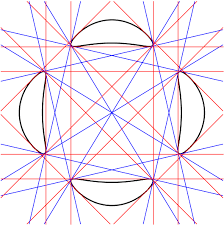
\includegraphics{images/trott_curve.png}
                \caption{The Trott curve and its $28$ bitangents.}
        \end{center}
\end{figure}
\begin{example}[Trott curve]\label{}\text{}
The \defn{Trott curve}\index{Trott curve} is given by
\begin{align*}
	12^2(x^4+y^4) - 15^2 (x^2+y^2) + 350 x^2y^2+81=0.
\end{align*}
This is a simple example of a nonsingular genus-$3$ curve with $28$ bitangents.
\end{example}

Curves of genus $4$ are intersections of a cubic and quadric in $\mathbf{P}^3$. Curves of genus $5$ are intersections of three quadrics in $\mathbf{P}^4$.

\subsection{Hurwitz curves.}
Hurwitz curves are the most symmetric curves of a given genus $g$. The group of automorphisms for the cases $g=0$ and $g=1$ are infinite. Thus, we would like to consider the automorphism group $G$ of curves of genus $g>1$. Hurwitz proved that
\begin{align*}
	\# G \le 84(g-1)
\end{align*}
in characteristic $0$. 
\begin{esquisse}
	Consider the orbifold Euler characteristic. Recall that the Euler characteristic is $\chi =n_2-n_1+n_0$ where $n_i$ is the number of cells of dimension $i$ (in a suitable cellular decomposition). The Euler characteristic of a compact orientable surface is $\chi = 2-2g$. An \defn{orbifold}\index{orbifold} is the quotient of a surface by a finite group.\footnote{That is, it is for our purposes.} If one has a point fixed by a subgroup $H$, then the quotient of this point by $H$ might be thought of as $1/\# H$ of a point. \iffalse Consider the unit disk. Take the automorphism of order $2$ that corresponds to a rotation by $\pi$. If\fi One can check that, if $S$ is a surface and $G$ is a finite group,
	\begin{align*}
		\chi(S/G) =  \frac{\chi(S)}{\# G}.
	\end{align*}
One can consider $S/G$ a surface, provided the action of $G$ is ``nice'' enough. That is, $S/G$ has a topological Euler characteristic and an orbifold Euler characteristic. Suppose that $S/G$ is a surface $T$ with conical singular points of orders $p_1,p_2,\hdots, p_m$. The orbifold Euler characteristic is the topological Euler characteristic minus $\sum_{i}^{}  (1-1/p_i)$.\footnote{What is happening here is that each conical singularity contributes $1$ to the topological Euler characteristic and $1/p_i$ to the orbifold one.} We want to show that the maximal value of the orbifold Euler characteristic is $-1/42$.

First, note that the topological Euler characteristic is $2-2h$ where $h$ is genus of the topological surface. One sees that $h=0$, since the orbifold Euler characteristic must be negative.\footnote{Recall that $g>1$.} Suppose that there are at most $2$ conical points $p_1$ and $p_2$. Then, again, the orbifold Euler characteristic will be positive. Suppose there are at least $4$ conical points. Then the orbifold Euler characteristic will be at most $-1/6$ (since $0$ is not possible), which is less than $-1/42$. Therefore, we look at the case where there are $3$ conical points $p_1$, $p_2$, and $p_3$. 

Suppose that there are no conical points of order $2$. If each point has an order of $3$, then the orbifold Euler characteristic is $0$. If two points are of order $3$ and one is of order $4$, then it is $-1/12< -1/42$. Thus, there is at least $1$ point of order $2$. One also sees that there cannot be more than $2$ points of order $2$, since that makes the orbifold Euler characteristic positive. That is, there is $1$ point of order $2$.

Suppose $p_2,p_3\ge 4$. If one has equality, then the orbifold Euler characteristic is $0$. If $p_2=4$ and $p_3=5$, then the orbifold Euler characteristic is $-1/20<-1/42$. Thus, one can assume that $p_1=2$, $p_2=3$, and $p_3\ge 3$. The possibilities for $p_3$ give
\begin{align*}
	\frac{1}{6},\ \frac{1}{12},\ \frac{1}{30},\ 0, \ -\frac{1}{42},\  -\frac{1}{24},\ \hdots
\end{align*}
for the orbifold Euler characteristic.

Therefore, if $\chi<0$, then $\chi\le -1/42$. Further, if $\chi \ne -1/42$, then $\chi \le -1/24$. Hence, if the orbifold Euler characteristic is negative (that is, if $g>1$), then 
\begin{align*}
	\frac{2-2g}{\# G}\le -\frac{1}{42}.
\end{align*}
This implies
\begin{align*}
	\# G\le 84(g-1).
\end{align*}
\end{esquisse}
In particular, $G$ is generated by $\alpha$, $\beta$, and $\gamma$ where $\alpha^2=1$, $\beta^3=1$, $\gamma^7=1$, and $\alpha\beta\gamma=1$. A finite group $G$ generated by $3$ elements with these properties is called a \defn{Hurwitz group}\index{Hurwitz group}.

 \begin{definition}[ ]\label{}\text{}
A \defn{Hurwitz curve}\index{Hurwitz curve} is a genus-$g$ curve with $84(g-1)$ automorphisms.
\end{definition}

\subsection{Examples of Hurwitz curves.}
One gets interesting information about genus $0$ or $1$ from the arguments of the previous section. If the genus is $g=0$, then the orbifold Euler characteristic is positive. The smallest orbifold Euler characteristic one gets is 
\begin{align*}
	2-\frac{1}{2}-\frac{2}{3}-\frac{4}{5}= \frac{1}{30} = \frac{2}{\# G}.
\end{align*}
This implies that there is a group of automorphisms of order $60$ that acts on $\mathbf{P}^1$. 

If $g=1$, then $\chi=0$. One can get this if there are no conical singularities, $4$ conical singularities of order $2$, $3$ conical singularities of order $3$, $1$ conical singularity of order $2$ and $2$ of order $4$, or $3$ conical singularities where the orders are $2$, $3$, and $6$.\footnote{These possibilities correspond to finite cyclic groups of orders $1$, $2$, $3$, $4$, and $6$ acting on an elliptic curve.} 

		Let us try to find the ``most symmetric'' curve of genus $g=2$. First, note that there isn't a genus-$2$ curve whose automorphism group has order $84$: Suppose that the automorphism group $G$ has order $84$. By the Sylow theorems, $G$ has a normal subgroup of order $7$. The group $G$ modulo this group of order $7$ is of order $12$ and has a normal subgroup of order $3$ or $4$. If it is of order $4$, then every element of order $2$ or $7$ is in the normal subgroup of order $28$, which has no elements of order $3$. Recall that any Hurwitz group has generators such that $\alpha^2 = \beta^3 = \gamma^7 = \alpha\beta\gamma = 1$. Therefore, one does not have a normal subgroup of order $4$. The order-$3$ normal subgroup case is similar: Every element of order $3$ or $7$ is contained in the normal subgroup of order $21$. Therefore, there is no Hurwitz group of order $84$.

		We also saw that if $\# G\ne 84(g-1)$, then $\# G \le 48(g-1)$. One sees that there is a curve whose automorphism group has order $48(g-1)=48$: Consider the double branched cover of $\mathbf{P}^1$ branched over $0$, $\infty$, $1$, $-1$, $i$, and $-i$.\footnote{One might think of these points as the vertices of an octahedron.} The subgroup of $\PSL_2(\mathbf{C})$ fixing these points is generated by
		\begin{align*}
			z&\longmapsto iz;\\
			z&\longmapsto \frac{z+1}{1-z}.
		\end{align*}
		Indeed, these generate a group of order $24$. The group of automorphisms is a central extension of this group in which the two branches are exchanged. This gives a group of order $48$ that acts on this hyperelliptic curve.

		There is a genus-$3$ Hurwitz curve that is given by the \defn{Klein quartic}\index{Klein quartic}:
		\begin{align*}
			x^3y + y^3z + z^3x=0.
		\end{align*}
		Indeed, this is nonsingular, and it is the only genus-$3$ curve whose automorphism group has order $84(g-1)=168$ up to isomorphism. Further, this automorphism group is the simple group $\PSL_{2}(\mathbf{F}_{7})$.\footnote{This is the smallest simple group after $\Ag_5$.} There is a manifest order-$3$ automorphism: $x\longmapsto y\longmapsto z\longmapsto x$. There are also order-$7$ automorphisms given by
		\begin{align*}
			x&\longmapsto \zeta^4x;\\
			y&\longmapsto \zeta^2y;\\
			z&\longmapsto \zeta z;
		\end{align*}
		where $\zeta$ is a $7$th root of unity. Determining the remaining automorphisms is quite difficult and, hence, omitted.

\begin{remark}
	In characteristic $p\ne 0$, the Euler characteristic behaves much differently than it does in characteristic $0$.\footnote{One defines the Euler characteristic in characteristic $p$ using \'etale cohomology.} Hence, the Hurwitz bound does not hold: The double cover of the projective line $y^2=x^p-x$ branched at all points defined over $\F_p$ has genus $g = (p-1)/2$ but is acted on by the group $\SL_{2}(\Z/p\Z)$ of order $p^3-p$.
\end{remark}

\subsection{Resolutions of curve singularities.}
We have seen that function fields of transcendence degree $1$ sort of correspond to nonsingular projective curves.\footnote{Hartshorne constructs a curve directly from a function field.} 

If a function field has transcendence degree $1$, then it is of the form $K(z_1,z_2)$ where $z_1$ is transcendental over $K$ and $f(z_1,z_2)=0$ for some $f$, which gives a possibly singular projective curve. We shall demonstrate that one can resolve the singularities of $f(z_1,z_2)=0$ by repeated blow ups.\footnote{We assert that $\chr K =0$, though the result holds in all characteristics.}

Assume that the singular point is $(0,0)\in  \mathbf{A}^2$. Consider the lowest-degree terms, say $a_ny^n + a_{n-1}xy^{n-1} + \cdots + a_1 x^{n-1}y + a_0 x^n$. The number $n$ is the \defn{multiplicity}\index{multiplicity of a singularity} of the singularity. The roots of this homogeneous polynomial given by the lowest-degree terms are in $\mathbf{P}^1$ and correspond to the ``directions'' of the singularity. Blowing up this point means separating these directions. Therefore, $1$ blow up reduces multiplicities unless all of the points are the same. In the latter case, this homogeneous polynomial is of the form $a_n(y+\alpha x)^n$.

Make the change of variables $y\longmapsto y-\alpha x$. Then, the degree-$n$ terms are given by only $y^n$.

\begin{example}[ ]\label{}\text{}
Let us blow up $y^2+x^9 + x^3y^5$ at $(0,0)$. This corresponds to either $x\longmapsto xy$, which does not produce any singularities, or $y\longmapsto xy$. In this case, one gets
\begin{align*}
	y^2 + x^7 + x^6y^5=0.
\end{align*}
One sees that, under this change of variables, monomials of the form $y^nx^\alpha$ are invariant (by $y^nx^\alpha\longmapsto y^nx^{\alpha+n}$ and dividing out by the common $x^n$). In general, one has $y^{n-\ell}x^\alpha \longmapsto y^{n-\ell}x^{\alpha-\ell}$. Hence, one can blow up until at least $1$ monomial has degree $n$. Then, one is in the previous case in which multiplicities can be reduced by blowing up.
\end{example}

However, one sees that the monomials of degree $n$ might be another $n$th power. Nevertheless, either the process terminates or the polynomial is transformed into a power series. In the latter case, the original polynomial is divisible by some $m$th power of a power series where $m\ge 2$.\footnote{An example of this is $f(x,y)= (y^2-y+x^2)^2$.} This is not possible, though, since the original polynomial $f(x,y)$ doesn't have repeated factors.\footnote{It is actually an irreducible curve.} Therefore, one has an algorithm for resolving singularities of an algebraic curve by blowing up.

\begin{remark}
	Subschemes can be defined by a polynomial with repeated factors; in this case, their singularities cannot be resolved by blowing up.
\end{remark}

\subsection{Newton's rotating ruler.}
Consider a polynomial $f(x,y)\in  \mathbf{C}[x,y]$ that is not a polynomial in $x$. Newton proved that $y$ is a power series in $x^{1/N}$ for some $N$. These are called \defn{Puiseux series}\index{Puiseux series}.\footnote{Puiseux series can have negative exponents, too.}

\begin{example}[ ]\label{}\text{}
If $f(x,y) = y^2-x^2 -x^3$, then
\begin{align*}
	y &= x\sqrt{1+x}\\
	  &= x \left( 1 + \frac{1}{2}x^{1/2} + \cdots \right). 
\end{align*}
\end{example}

\begin{esquisse}
	Suppose that $f$ has a $y^n$ term but not $y^i$ for $i<n$. Draw a square lattice of monomials. Mark all monomials $x^iy^j$ that occur in $f$. Get a ruler.\footnote{This ruler will transfigure to become Newton's rotating ruler.} Place it vertically on the left of the lattice. Rotate it counterclockwise about the $y^n$ point until it reaches the first marked point. Draw a line through these points. Rotate about this point. Repeat. This process will generate a \defn{Newton polygon}\index{Newton polygon}.

	One notices that the line that one draws might not pass through a point on each horizontal. Hence, one introduces extra points by $x\longmapsto x^{1/r}$ for a suitable $r$. Write the next monomial through which the line crosses $y^{n-1}x^m$. One can call the terms on the first line of the Newton polygon (which, now, passes through a point on each horizontal) the ``smallest-degree terms.'' Put $\deg y = m$ and $\deg x = 1$. The monomials on this line give a homogeneous polynomial in $y$ and $x^m$. Factorize this to $(y-\alpha x^m) (y-\beta x^m)\cdots$. Then, with $y\longmapsto y+\alpha x^m$, this polynomial becomes $y(y-\gamma x^m)\cdots$. Notice that there is no term in $x^{mn}$.

	Now, with $y\longmapsto x^my$, all of the terms are divisible by $x^{mn}$, so one divides out by $x^{mn}$. One sees that all of the points on that line are pushed all the way to the left. Now, if any of the coefficients are nonzero, then the exponent on $y$ is less than $n$; then, one repeats with this smaller exponent. This happens when the first root in the factorization has multiplicity less than $n$. Hence, one focuses on the case when the multiplicity of this root is $n$.\footnote{Typically, this occurs when $n=1$.}

	In this case, the coefficient on $y^n$ is $1$. Further, every other coefficient on the line is $0$. Then, Newton's ruler has not met a marked point, so it rotates on. Therefore, either $n$ is decreased or the ruler is rotated counterclockwise. This rotation process\footnote{The rotation process here corresponds to $y\longmapsto y + *x^m$.} either continues ad infinitum or the smallest power of $y$ is reduced. There are finitely many times that one can reduce the exponent on $y$, so the rotation process will continue forever.

	When it continues on and on, one sees that the following sequence of variable changes is happening:
	\begin{align*}
		y &\longmapsto y + *x;\\
		y &\longmapsto y + *x^2;\\
		y &\longmapsto y + *x^3;
	\end{align*}
	etc. That is, one has $y\longmapsto y + *x + *x^2 + *x^3 + \cdots$. Then, all monomials $y^ix^j$ for $i< n$ vanish. Now, the series is divisible by $y$, so the original $f(x,y)$ is divisible by $y$ minus some power series in $x^{1/r}$ for some $r$. Thus, $y$ is a power series in $x^{1/r}$ that satisfies $f(x,y)=0$.
\end{esquisse}

\begin{corollary}[ ]\label{}\text{}
The field of Puiseux series\index{Puiseux series}
\begin{align*}
	K = \bigcup_{n>0} \mathbf{C} (\!(z^{1/n})\!)
\end{align*}
is algebraically closed.
\end{corollary}

If one has a polynomial in $y$ whose coefficients are Puiseux series in $z$, its roots are Puiseux series. That is, $K$ is algebraically closed.

The field $K$ is a \defn{quasifinite field}\index{quasifinite field}. That is, its absolute Galois group is $\widehat{\mathbf{Z}}$, which is the absolute Galois group of $\mathbf{F}_{p}$.

\subsection{Hilbert polynomials.}
Suppose $M=\bigoplus_{n}M_n$ is a finitely-generated graded module over a graded ring $R = K[z_1,\hdots, z_m]/I$ where $\deg z_i = d_i >0$. If $R$ is the graded ring of some projective variety, the ``growth rate'' of the $M_n$s might give some information about the variety.

Consider
\begin{align*}
	f_M(z) :=  \sum_{n}^{} z^n\dim_K(M_n)
\end{align*}
where $\dim_K(M_n)$ is the dimension of $M_n$ as a $K$--vector space. First, notice that $f_M$ is a \index{rational function}rational function. Consider the exact sequence
\[
\begin{tikzcd}
	0\ar[r]&\Ker z_m \ar[r] & M \ar[r,"\times z_m"]& M(d_m) \ar[r] & M(d_m)/z_m M \ar[r]& 0. 
\end{tikzcd}
\]
Note that $M(d_m)$ means $M$ with its grading shifted by $d_m$. Since this is an exact sequence of vector spaces, one gets a relation between the dimensions of these vector spaces. Furthermore, $\Ker z_m$ and $M(d_m)/z_m M$ are $R/(z_m)$-modules. Also,
\begin{align*}
	f_{M(d_m)}(z) = z^{d_m} f_M(z).
\end{align*}
Thus, by induction, $(1-z^{-d_m})f_M$ is a rational function. Further, $f_M$ is a rational function with denominator dividing $(1-z^{d_1})\cdots(1-z^{d_m})$.

Let us focus on the case $d_i=1$ for all $i$. Then, the denominator is $(1-z)^m$, and the coefficients of $z_i$ for $i\ge 0$ in the expansion of $1/(1-z)^m$ are given by a polynomial in $i$. Therefore, $\dim_k (M_n)$ is a polynomial in $n$ for $n>0$ large. This is called the \defn{Hilbert polynomial}\index{Hilbert polynomial} of $M$. It describes how rapidly the graded pieces of $M$ grow in large degree.

Write $g(n) := \dim_K(M_n)$ for the Hilbert polynomial of $M$. Though its coefficients are not necessarily integers, the restriction
\begin{align*}
	g:\mathbf{Z}\longrightarrow \mathbf{Z}
\end{align*}
is well defined; that is, $g$ is integer-valued. Let us see what integer-valued polynomials look like. Clearly, $a_mz^m + \cdots + a_1z + a_0$ is an integer if $z$ is an integer and $a_i$ is an integer for all $i$. However, an integer-valued function does not need integral coefficients: Consider
\begin{align*}
	\frac{z(z-1)}{2}.
\end{align*}

Notice that the binomial coefficients
\begin{align*}
	1 &= \binom{z}{0};\\
	z &= \binom{z}{1};\\
	\frac{z(z-1)}{2} &= \binom{z}{2};\\
	\frac{z(z-1) (z-2)}{3!}&= \binom{z}{3};
\end{align*}
are integer-valued. We shall demonstrate that these span the integer-valued polynomials. Write 
\begin{align*}
	g_n(z) := \binom{z}{n}.
\end{align*}
Then
\begin{center}
	\begin{tabular}{cccccccc}
		$z$&0&1&2&3&4&5\\
    		\midrule
		 $g_0(z)$& $1$ &     &     &    \\
		 $g_1(z)$& $0$ & $1$ &     &    \\
		 $g_2(z)$& $0$ & $0$ & $1$ &    \\
		 $g_3(z)$& $0$ & $0$ & $0$ & $1$\\
		 $g_4(z)$& $0$ & $0$ & $0$ & $0$ & $1$\\
		 $g_5(z)$& $0$ & $0$ & $0$ & $0$ & $0$ & $1$
	\end{tabular}
\end{center}
Suppose $f(n)$ is a degree-$\ell$ integer-valued polynomial. Then, one can choose coefficients such that
\begin{align*}
	f(n) -  a_0g_0(n) -  a_1g_1(n) - \cdots - a_\ell g_\ell (n) =0
\end{align*}
for $n = 0,\hdots, \ell$. The above is a polynomial of degree $\ell$ that vanishes at $\ell + 1$ points, so it is $0$. Notice that the leading coefficient of $f$ is $a_\ell n^\ell / \ell!$ where $a_\ell$ is an integer.\footnote{This integer will give the degree of projective varieties.}

\begin{remark}
In the construction of the Hilbert polynomial, we used $\dim_K(M_n)$ because it was additive on short exact sequences. Any other measure of the ``size'' of $M_n$ that is additive on short exact sequences can give a variation on the Hilbert polynomial of $M$.	
\end{remark}

\subsection{The degree of a projective variety.}
\index{degree of a projective variety}
Suppose that $V\subseteq \mathbf{P}^n$ is a projective variety. If $V$ is a hypersurface, it is given by $f(z_0,\hdots,z_n)=0$ for a polynomial $f$. One defines
\begin{align*}
	\deg V := \deg f.
\end{align*}

\iffalse
Most of the time, if $V$ has codimension greater than $1$, then $\deg V$ is the number of intersection points of $V$ with a hyperplane section $H$ or the number of intersections of $V$ with a linear variety of codimension $\dim V$. However, one requires the hyperplane section or linear variety to be in ``general position,'' whatever that means.
\fi

One used to define $\deg V$ in terms of intersections with hyperplane sections or linear varieties, but these ``definitions'' had many caveats to them.

Suppose $V$ corresponds to an ideal $I$ of $K[z_0,\hdots, z_n]=R$.\footnote{That is, $V$ is the set of roots of $I$.} Now, $R/I$ is a graded ring, so it has a Hilbert polynomial. The degree of this Hilbert polynomial is $\dim V$. This is closely related to the following theorem from commutative algebra.

\begin{theorem}[ ]\label{}\index{}\text{}
Let $R$ be a local ring with maximal ideal $\mathfrak{m}$. Then, $\dim R$ is $1$ plus the degree of the Hilbert polynomial of $\mathfrak{m}^n / \mathfrak{m}^{n+1}$.
\end{theorem}

If $d:=\dim V$, the leading coefficient of the Hilbert polynomial is $\alpha z^d/d!$ where $\alpha\in \Z$. One defines
\begin{align*}
	\deg V := \alpha.
\end{align*}
Notice that $\alpha>0$ since the Hilbert polynomial takes on positive values for large inputs.

\begin{remark}
	The degree defined this way is a well-defined invariant of a projective variety together with its embedding in projective space.
\end{remark}

\begin{example}[ ]\label{}\text{}
Suppose that $V=\mathbf{P}^n$. Hence, one considers the graded ring $K[z_0,\hdots,z_n]/(0)=K[z_0,\hdots,z_n]$. The Hilbert polynomial of this is
\begin{align*}
	\binom{n+z}{n} = \frac{z^n}{n!} + \cdots.
\end{align*}
This counts the monomials of degree $z$. One sees that $\dim V = n$ and $\deg V = 1$. 
\end{example}

\begin{example}[ ]\label{}\text{}
Consider a hypersurface of a degree-$d$ polynomial $f(z_0,\hdots, z_n)$. Now, one considers $K[z_0,\hdots, z_n]/(f)$. The Hilbert polynomial of this is
\begin{align*}
	\binom{n+z}{n} - \binom{n+z-d}{n}  = d \frac{z^{n-1}}{(n-1)!} + \cdots,
\end{align*}
so the dimension of the hypersurface is $n-1$ and the degree of the hypersurface is $d$.
\end{example}

\begin{example}[Twisted cubic]\label{}\text{}
\index{twisted cubic} Recall that the twisted cubic is given by
\begin{align*}
	wz &= xy;\\
	x^2 &= wy;\\
	y^2 &= xz.
\end{align*}
One can kill off $x^2$, $y^2$, and $xy$, so a basis for the relevant quotient ring is 
\[
	\{w^iz^{z- i}, w^ixz^{z- i -1}, w^iyz^{z-i-1}\}. % ``Overfull \hbox'' . . . 
\] 
There are $( z+ 1)+z +  z = 3z + 1$ of these, so the Hilbert polynomial is $3z+1$. Therefore, the twisted cubic has dimension $1$ and degree $3$.
\end{example}

\begin{remark}
	The twisted cubic is isomorphic to the projective line, which is of degree $1$. Thus, the degree depends on the embedding.
\end{remark}

The \defn{Euler polynomial}\index{Euler polynomial} of $V$, $\chi(V)$, is the constant term of the Hilbert polynomial. The Euler polynomial depends on only the abstract variety, not on the variety's embedding. It is the Euler characteristic of the sheaf of rings of $V$. People didn't use $\chi(V)$; they used the \defn{arithmetic genus}\index{arithmetic genus}:
\begin{align*}
	(-1)^{\dim V}  (\chi(V)-1).
\end{align*}
However, the Euler characteristic is ``better,'' since
\begin{align*}
	\chi(V\times W) = \chi (V)\chi (W).
\end{align*}

\begin{problem}
	Determine the arithmetic genus of a plane curve of degree $d$.
\end{problem}

The Hilbert polynomial of this plane curve is
\begin{align*}
	\binom{2+z}{2} - \binom{2+z-d}{2} = dz + 1 - \frac{(2-d) (1-d)}{2},
\end{align*}
so the arithmetic genus is $(2-d) (1-d)/2$.

Robin Hartshorne proved the following theorem.\footnote{``Connectedness of the Hilbert scheme,'' 1963.}

\begin{theorem}[Hartshorne]\label{}\index{}\text{}
Let $S$ be a Noetherian prescheme, let $n$ be an integer, and let $\rho(z)\in\Q [z]$ be a polynomial. If $S$ is connected, then the Hilbert scheme $\Hilb^\rho(\mathbf{P}^n_S/S)$ is connected.
\end{theorem}

This implies that the Hilbert polynomial is, essentially, the only continuous invariant of things in projective space.

\subsection{B\'ezout's theorem.}
Here is B\'ezout's theorem in its simplest form.
\begin{theorem}[B\'ezout]\label{b_1}\index{B\'ezout's theorem}\text{}
Curves of degrees $m$ and $n$ intersect at $mn$ points.
\end{theorem}
However, this is wrong as stated. Two distinct parallel lines, for example, do not intersect. To patch this, one includes points at infinity.\footnote{That is, one works in projective space.} The curves $y=0$ and $y=x^2+1$ do not intersect over $\R$, but they do over $\C$. Thus, one needs to work over an algebraically closed field. Thirdly, the curves must not have components in common. Further, the curves $y=0$ and $y=x^2$ intersect at one point, so one needs to consider multiplicities.\footnote{Things get even more complicated here when one considers, for example, $y^3-x^4=0$ and $y^5 - x^6=0$.} It is challenging, though, to define ``multiplicity.''

Let's try again.

\begin{theorem}[B\'ezout]\label{b_2}\index{B\'ezout's theorem}\text{}
Two distinct irreducible curves in $\mathbf{P}^2\mathbf{C}$ of degress $m$ and $n$ intersect at $mn$ points up to multiplicity.
\end{theorem}

Further, one might want that $n$ distinct hypersurfaces in $\mathbf{P}^n\mathbf{C}$ of degrees $d_1,\hdots, d_n$ usually\footnote{That is, when the intersections are not of the wrong dimension.} intersect at $d_1\cdots d_n$.

One might ask whether the intersection of two algebraic sets of degrees $m$ and $n$ is of degree $mn$, setting aside the definition of the degree of an algebraic set. Oftentimes, it is.\footnote{Recall the informal ``perturbation proof'' from \cref{s_3}. Even though it doesn't prove anything, it gives one the impression that B\'ezout's theorem is true, and it extends to higher dimensions.} 

Now, one recalls the theory of finitely-generated modules over Noetherian rings. Suppose $M$ is a finitely-generated module over a Noetherian ring $R$. One can filter $M$
\begin{align*}
	0=M_0 \subset M_1\subset \cdots\subset M_n=M
\end{align*}
such that $M_i/M_{i-1} \isomto R/\mathfrak{p}$ where $\mathfrak{p}$ is a prime ideal.
\begin{esquisse}
	Choose $I$ maximal among ideals such that $R/I$ is isomorphic to a submodule of $M$. Check that $I$ is prime. Set $M_1\isomto R/I$. Induction.
\end{esquisse}

One would like to define the multiplicity of $R/\mathfrak{p}$ in $M$ to be the number of times $R/\mathfrak{p}\isomto M_i/M_{i-1}$.

\begin{example}[ ]\label{}\text{}
Take $R=\mathbf{Z}$ and $M$ a finite (abelian) group. Then $R/\mathfrak{p} \isomto \Z/2\Z,\Z/3\Z,$ etc. If $\# M = p_1^{n_1}\cdots p_\ell^{n_\ell}$, the number of times $\Z/p_1\Z$ is in $M$ is $n_1$. 
\end{example}

\begin{example}[ ]\label{fail_1}\text{}
Let $M=\mathbf{Z}$. In the filtration $0=M_0\subset M_1=\mathbf{Z}$, $\mathbf{Z}/2\mathbf{Z}$ doesn't occur. However, in the filtration $0\subset 2\mathbf{Z}\subset \mathbf{Z}$, $\mathbf{Z}/2\mathbf{Z}$ occurs once.
\end{example}

\begin{remark}
	Therefore, one cannot define ``multiplicity'' as above for all primes: It depends on the filtration.
\end{remark}

\begin{example}[ ]\label{}\text{}
Let $M$ be a finitely-generated module over $\mathbf{Z}$. Then, the multiplicity of $\mathbf{Z}/(0)$ in $M$ is defined: It is the rank of $M$, which one might determine by tensoring with $\mathbf{Q}$ and taking the dimension of the resulting vector space.
\end{example}

Look at the prime ideals $\mathfrak{p}_1,\mathfrak{p}_2,\hdots$ with $R/\mathfrak{p}_i$ in a filtration of $M$. If $\mathfrak{p}_j$ is minimal, one gets a well-behaved multiplicity. Notice that, in \cref{fail_1}, $(0)$ is minimal but $(2)$ is not. If $\mathfrak{p}$ is minimal, its \defn{multiplicity}\index{multiplicity of an ideal} is the length of $M_{\mathfrak{p}}$ over $R_{\mathfrak{p}}$, where $R_{\mathfrak{p}}$ is the localization of $R$ at $\mathfrak{p}$, etc.

Let $R=\mathbf{C}[z_1,z_2]$. Prime ideals of $R$ correspond to points, curves, and the plane. Suppose one draws the prime ideals that occur in a filtration of an $R$-module $M$. The minimal primes are ``maximal varieties.''\footnote{That is, if one has a point and a curve that intersects that point, the minimal prime there is the curve.} One might think of this set of primes as the annihilator of $M$, an ideal that corresponds to an algebraic set that splits up into irreducible subsets that correspond to the minimal primes.

There is a similar theorem for graded modules over graded rings, in which the only difference is that one might shift the degree of $R/\mathfrak{p}$ by an integer $\ell$. 

Now, let us state and prove B\'ezout's theorem.

\begin{theorem}[B\'ezout]\label{b_3}\index{B\'ezout's theorem}\text{}
Let $Y$ be a variety in $\mathbf{P}^n$. Let $H$ be a hypersurface given by $f(z_0,\hdots, z_n)=0$. Suppose that $Y$ is not contained in $H$. Then,
\begin{align*}
	\sum_{j}^{} \mult(Y, H; Z_j) \deg (Z_j) = \deg  (Y)\deg (H)
\end{align*}
where $Y\cap H$ is a union of irreducible components $Z_j$ and $\mult(Y,H;Z_j)$ is the multiplicity of the intersection of $Y$ and $H$ at $Z_j$.
\end{theorem}

\begin{proof}
Consider the exact sequence of modules
\[
\begin{tikzcd}
	0\ar[r] & K[z_0,\hdots,z_n] / I_Y \ar[r, "\times f"] & K[z_0,\hdots, z_n] /I_Y \ar[r] & K[z_0,\hdots, z_n]/(I_Y, f)\ar[r] &0
\end{tikzcd}
\]
in which the degree of the second term is shifted by $-\deg f$. Note that the Hilbert polynomials of these terms are related: The Hilbert polynomial of the last term is $P_Y(z) - P_Y (z-d)$ where $d=\deg f$. The Hilbert polynomial of $Y$ is
\begin{align*}
	P_Y(z) =  \frac{\deg(Y)z^{\dim Y}}{(\dim Y)^!}+\cdots
\end{align*}
and
\begin{align*}
	P_Y(z-d) =  \frac{\deg(Y) (z-d)^{\dim Y}}{(\dim Y)!}+\cdots.
\end{align*}
Thus, the leading term of $P_Y(z)-P_Y (z-d)$ is $d = \deg(Y) z^{\dim Y-1}/ (\dim Y- 1)!$, so the Hilbert polynomial of $K[z_0,\hdots,z_n]/(I_Y,f)$ has leading term
\begin{align*}
	\deg(H)\deg (Y)  \frac{z^{\dim Y\cap H}}{(\dim Y\cap H)!}.
\end{align*}
This implies that $\dim (Y\cap H) =\dim (Y)-1$. 

The module $M=K[z_0,\hdots, z_n]/(I_Y, f)$ has a filtration 
\begin{align*}
	0  = M_0\subset M_1\subset\cdots \subset M_k = M
\end{align*}
such that the quotients are of the form $R/\mathfrak{q}_i(\ell_i)$ for some graded prime ideal $\mathfrak{q}_i$. Shifting by $\ell_i$ does not change the leading coefficient since it is comes with the dominant term asymptotically. Thus, the Hilbert polynomial of each $R/\mathfrak{q}_i(\ell_i)$ has leading term
\[
	\frac{\deg (Z_i)}{(\dim Z_i)!}z^{\dim Z_i}.
\]
Quoting dimension theory, $\dim Z_i = \dim (Y)-1$. Hence, 
\begin{align*}
	\deg(H)\deg (Y) =  \sum_{j}^{} \deg(Z_j) \mult (R/\mathfrak{q}_j(\ell_j) \textrm{ in $K[z_0,\hdots, z_n]/(I_Y,f)$}).
\end{align*}
The claim is that this last term is the multiplicity of the corresponding intersection.
\begin{quote}
	\small There's an old joke about a target shooter who got 100 percent in his target shooting. He would fire at the target and, then, draw a circle around the bullet to indicate that that was the target at which he was firing. 
\end{quote}
We shall employ the same technique. Notice that we haven't defined the multiplicity of an intersection yet. Drawing inspiration from the target shooter, we define the multiplicity of an intersection such that the result holds. 
\end{proof}


\section{Schemes}
\iffalse
\begin{figure}
\begin{center}
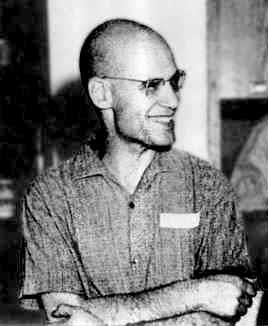
\includegraphics[scale=0.8]{images/groth}
\caption{Alexander Grothendieck.}
\end{center}
\end{figure}
\fi
\subsection{Introduction. Presheaves. Sheaves.}
Affine varieties over a field $K$ correspond to commutative rings $R$ that satisfy the following properties:
\begin{enumerate}
	\item $R$ is a $K$-algebra;
	\item $R$ is finitely-generated as an algebra;
	\item $R$ is reduced.
\end{enumerate}
The coordinate ring of an affine variety has these properties. Further, one can construct an affine variety from a commutative ring with these properties.

The coordinate ring of a line $K[z]$ behaves similarly to $\mathbf{Z}$ or algebraic number fields such as $\mathbf{Z}[i]$. It was noticed in the nineteenth century that the theory of algebraic number fields was very similar to the theory of curves over finite fields. Hence, one wants algebraic geometry to include these things, so we don't want to require that $R$ is an algebra over a field. 

One might want to consider the localization of the ring of rational functions $K(z)$ at the ideal $(z)$. However, this is not finitely-generated as an algebra.

Further, one might want to intersect curves $y=x^2$ and $y=0$. Then, one considers the ring $K[z_1,z_2]/(z_2,z_1^2-z_2) \isomto K[z]/ (z^2)$. Classically, one replaces this with $K[z]/(z) = K$. However, when one does this, one loses information about the intersection. This replacement is the coordinate ring of a point, and while these curves intersect at a point, that point is really a ``double point.'' The ring $K[z]/(z^2)$ is two-dimensional, so it keeps track of the ``double point''; however, it has nilpotent elements.

One sees the benefit in abandoning these extra conditions. Hence, one wants to define some generalization of an affine variety that corresponds to commutative rings. We shall call these mysterious things ``affine schemes.''\index{affine scheme} However, to define them, one needs to look into the theory of sheaves.

\index{sheaf}Sheaves were introduced by Jean Leray circa 1950. Thereafter, Jean-Pierre Serre and Henri Cartan used them to study analytic varieties. Serre introduced sheaves to algebraic geometry in his famous ``Faisceaux Algébriques Cohérents'' of 1955.\footnote{FAC is a superb introduction to sheaf theory.}

Prior to the introduction of sheaves, people found all sorts of invariants in algebraic geometry. Take, for example, the \index{arithmetic genus}arithmetic genus, which didn't seem to depend on a surface's embedding in projective space. It was hard to define or compute, though: One of its definitions was
\begin{align*}
	p\textsubscript{a} = \binom{\mu_0-1}{2} - (\mu_0 - 4) \varepsilon_0 + \frac{\varepsilon_1}{2} - \varepsilon_0+2t
\end{align*}
where these numbers are some rather strangely-defined invariants.\footnote{This was the definition for two dimensions. Good luck generalizing it.} With sheaves, the arithmetic genus of a surface is
\begin{align*}
	p\textsubscript{a} = \chi -1
\end{align*}
where the Euler characteristic $\chi$ is given by an alternating sum of dimensions of sheaf cohomology groups.

Another such invariant was the \defn{irregularity}\index{irregularity of a surface} of a surface. The irregularity was a weird thing that was related to the difference between the arithmetic and geometric genuses. However, with sheaves, it is, simply, the dimension of the first sheaf cohomology group of the structure sheaf. One extends this to higher dimensions by considering the dimension of higher sheaf cohomology groups. More generally, one defines the \defn{Hodge number}\index{Hodge number} 
\begin{align*}
	{\h}^{pq}(X) := \dim \HH^q(X,\Omega^p) 
\end{align*}
as the dimension of the $q$th homohology group of a sheaf of $p$-forms over a surface.

\begin{example}[Motivation]\label{}\text{}
Suppose $X$ is a topological space with an open set $U$. Let $\mathscr{F}(U)$ be the continuous functions from $U$ to $\mathbf{R}$. That is, $\mathscr{F}$ goes from open sets to abelian groups. One will call $\mathscr{F}$ a (pre)sheaf of abelian groups. 

If $V$ and $U$ are open sets and $V\subseteq U$, there is a restriction map
\begin{align*}
	\rho_{U}^V : \mathscr{F}(U)  \longrightarrow \mathscr{F}(V).
\end{align*}
Given open sets $W\subseteq V\subseteq U$, the restriction map $\rho$ makes
\[
\begin{tikzcd}
	\mathscr{F}(U)\ar[r,"\rho"] \ar[dr,"\rho", swap] &  \mathscr{F}(V)\ar[d,"\rho"] \\
						   & \mathscr{F}(W)
\end{tikzcd}
\]
commute. That is, $\rho_{U}^W = \rho_{V}^W \rho_{U}^V$. Further, $\rho_{U}^U$ is the identity.

A \defn{presheaf}\index{presheaf} of abelian groups is a map
\begin{align*}
	\mathscr{F} : \textrm{open subsets of $X$} \longrightarrow \textrm{abelian groups}
\end{align*}
together with restriction maps $\rho_{U}^V : \mathscr{F}(U) \longrightarrow  \mathscr{F}(V)$ for all open sets $U\subseteq V$ satisfying the above conditions. 
\end{example}

One can think of $\mathscr{F}$ as a contravariant functor from $\catn{Op}_X$ to $\catn{Ab}$. The objects of $\catn{Op}_X$ are open sets; further, there is $1$ morphism $U\longrightarrow V$ if $U\subseteq V$ and $0$ otherwise. One sees that $\mathscr{F}$ is assigning an abelian group to every open set and giving a map from the abelian group of $V$ to the abelian group of $U$ whenever $U\subseteq V$.

\begin{remark}
	This indicates that one can replace $\catn{Op}_X$ with another category and still define presheaves.\footnote{And similarly for $\catn{Ab}$.} Grothendieck did this to define \'etale cohomology.
\end{remark}

\begin{example}[Presheaves]\label{}\text{}
\begin{enumerate}
	\item Let $X$ be a smooth manifold. Let $\mathscr{F}(U)$ be the smooth vector fields on $U$. Not only is $\mathscr{F}$ a presheaf, $\mathscr{F}$ is a sheaf.
	\item Let $X$ be an affine variety. Let $\mathscr{F}(U)$ be the regular functions on $U$.
	\item Let $X$ be a Riemann surface. Let $\mathscr{F}(U)$ be the holomorphic functions on $U$. Riemann surfaces can be viewed as complex manifolds, smooth real manifolds, or topological manifolds. One gets different sheaves of functions from these perspectives.
	\item Let $\mathscr{F}(U) = A$ be a fixed abelian group. This is a presheaf.\footnote{This is not true for all definitions of ``presheaf.'' For example, Hartshorne adds the condition that $\mathscr{F}(\emptyset) = 0$.}
\end{enumerate}
\end{example}


Suppose $U$ is a union of open sets $U_\alpha$. A presheaf $\mathscr{F}$ is \defn{separated}\index{separated presheaf} if the image of $f$ in all $\rho_{U}^{U_\alpha}$ is $0$ implies $f=0$ for all $f\in \mathscr{F}(U)$. 

Suppose that $\mathscr{F}$ is separated. Suppose $f_\alpha,f_\beta\in \mathscr{F}(U_\beta)$ have the same image in $\mathscr{F}(U_\alpha\cap U_\beta)$. If one can find $f\in \mathscr{F}(U)$ with images $f_\alpha$ in $\mathscr{F}(U_\alpha)$, then $\mathscr{F}$ is a \defn{sheaf}\index{sheaf}.

\begin{example}[Presheaves that are not sheaves]\label{}\text{}
\begin{enumerate}
	\item Let $\mathscr{F}(U) = A$ for a fixed abelian group $A\ne 0$. A sheaf satisfies $\mathscr{F}(\emptyset) = 0$.
	\item Let
		\begin{align*}
			\mathscr{F}(U) = 
			 \begin{cases}
				 0&U=\emptyset\\
				 A&\textrm{otherwise.}
			\end{cases}
		\end{align*}
		Let $U = U_1\sqcup U_2$. Then $\mathscr{F}(U) =A$, but, if $\mathscr{F}$ were a sheaf, then $\mathscr{F}(U) =  \mathscr{F}(U_1)\times \mathscr{F}(U_2) = A\times A$.
\end{enumerate}

A presheaf $\mathscr{F}$ is a sheaf if the following sequence is exact:
\[
\begin{tikzcd}
	0 \ar[r] & \mathscr{F}(U) \ar[r] & \displaystyle\prod_\alpha  \mathscr{F}(U_\alpha) \ar[r, yshift = 0.5 ex] \ar[r, yshift = -0.5 ex] & \displaystyle\prod_{\alpha,\beta}  \mathscr{F}(U_\alpha\cap U_\beta).
\end{tikzcd}
\]
Note that 
\[
\begin{tikzcd}
	A\ar[r] &A\times A \ar[r, yshift = 0.5 ex] \ar[r, yshift = -0.5 ex] & 0 
\end{tikzcd}
\]
is not exact.
\end{example}

By the way, an element $s\in \mathscr{F}(U)$ is called a \defn{section}\index{section} and an element $s\in \mathscr{F}(X)=: \Gamma(\mathscr{F})$ is called a \defn{global section}\index{global section}.

\subsection{\'Etale spaces.}
Sheaves seem to be an unnecessarily complicated and abstract way to describe functions on a space. Of course, this isn't the case.

\begin{example}[ ]\label{}\text{}
The points of the affine line $\mathbf{C}$ correspond to the maximal ideals of the ring $\mathbf{C}[z]$.\footnote{The point $\alpha\in \mathbf{C}$ corresponds to the maximal ideal $(z-\alpha)$.} Given $f\in \mathbf{C}[z]$, define
\begin{align*}
	U(f) := \{\alpha : f(\alpha)\ne 0\}.
\end{align*}
Then, open sets have a basis $\{U(f)\}$ in the Zariski topology. Further, the ring of regular functions of an open set is given as follows: 
\begin{align*}
	\mathscr{F}(U(f)) = \{g/f^n: g\in \C[z]\}.
\end{align*}

Let us replace $\mathbf{C}[z]$ with $\mathbf{Z}$. The maximal ideals of $\mathbf{Z}$ are given by
\begin{align*}
	\specmax\mathbf{Z} = \{(2),  (3),\hdots\}.
\end{align*}
This set is called the \defn{maximal spectrum}\index{maximal spectrum} of $\mathbf{Z}$. Given $f\in \mathbf{Z}$, define 
\begin{align*}
	U(f) := \{\mathfrak{m}: f\notin  \mathfrak{m}\}.
\end{align*}
Then, one gets a basis of open sets $\{U(f)\}$. Now, define
\begin{align*}
	\mathscr{F}(U(f)) := \{ g/f^n : g\in \mathbf{Z}\}.
\end{align*}

One pretends that an integer is a function on the space $\specmax \mathbf{Z}$. One notes the difference, though: $f\in \C[z]$ has values in $\mathbf{C}$ at all points of $\mathbf{C} = \mathbf{C}[z]/(z-\alpha)$, but $f\in \mathbf{Z}$ has values in $\mathbf{Z}/(p)$, which varies as the point varies. Nevertheless, $\mathscr{F}$ satisfies the sheaf property.\footnote{This fact comes down to the fundamental theorem of arithmetic.}
\end{example}

Sheaves of sets behave similarly to sets; likewise, sheaves of abelian groups behave similarly to abelian groups. Hence, one can form a category of sheaves of sets and of sheaves of abelian groups. Given sheaves $\mathscr{F}$ and $\mathscr{G}$, one has a morphism by defining a morphism $\mathscr{F}(U) \longrightarrow \mathscr{G}(U)$ for all open sets $U$ that is compatible with the restriction map: Given open sets $V\subseteq U$,
\[
\begin{tikzcd}
	\mathscr{F}(U)\ar[d,"\rho", swap] \ar[r]&  \mathscr{G}(U)  \ar[d,"\rho"] \\
	\mathscr{F}(V) \ar[r]&  \mathscr{G}(V)
\end{tikzcd}
\]
commutes. Hence, sheaves comprise a category.

The category of sheaves of sets is a sort of weak model of set theory. It is called a \defn{topos}\index{topos}: One does set theory with sheaves over a topological space instead of sets.

Suppose
\[
\begin{tikzcd}
	0\ar[r]&A\ar[r]&B\ar[r]&C\ar[r]&0
\end{tikzcd}
\]
is an exact sequence of abelian groups. What this means is clear. Now, what does it mean for
\[
\begin{tikzcd}
        0\ar[r]&\mathscr{A}\ar[r]&\mathscr{B}\ar[r]&\mathscr{C}\ar[r]&0,
\end{tikzcd}
\]
a sequence of sheaves, to be exact? The obvious guess is that
\[
\begin{tikzcd}
	0\ar[r]&\mathscr{A}(U)\ar[r]&\mathscr{B}(U)\ar[r]&\mathscr{C}(U)\ar[r]&0
\end{tikzcd}
\]
is exact for all open sets $U$. This is wrong: While this is okay for saying that $\mathscr{A}\longrightarrow \mathscr{B}$ is injective, it is not for saying that $\mathscr{B} \longrightarrow \mathscr{C}$ is surjective.

\begin{example}[ ]\label{}\text{}
Let $X$ be a circle. Let $X_1=X$ and $X_2$ be a circle winding around $X$ twice. Let $\mathscr{F}_1(U)$ be the sections from $U$ to $X_1$ and $\mathscr{F}_2(U)$ be the sections from $U$ to $X_2$. These are sheaves. There is a natural surjective map from $X_2$ to $X_1$ (and a map from $X_1$ to $X$), whence one gets a natural map $\mathscr{F}_2\longrightarrow \mathscr{F}_1$. Note that $\mathscr{F}_2(X) \longrightarrow \mathscr{F}_1(X)$ is not surjective: $\mathscr{F}_1(X)$ is a point and $\mathscr{F}_2(X)$ is empty, since there are no continuous maps from $X$ to $X_2$ that are sections of it.

Hence, one has two different ways to talk about surjectivity depending on whether one looks at $X_2\longrightarrow X_1$ or $\mathscr{F}_2(X) \longrightarrow \mathscr{F}_1(X)$. These correspond to local and global notions respectively, and it turns out that one should work with a local definition. 
\end{example}

Suppose one has a continuous map from $A$ to $X$. One can construct a sheaf by letting $\mathscr{F}(U)$ be continuous sections from $U$ to $A$. Suppose further that one has a continuous map from $B$ to $X$. If $\mathscr{F}$ is the ``sheaf of $A$'' and $\mathscr{G}$ is the ``sheaf of $B$,'' a continuous map from $A$ to $B$ such that
\[
\begin{tikzcd}
	A \ar[d]\ar[r] &B\ar[dl]\\X
\end{tikzcd}
\]
commutes induces a map $\mathscr{F}\longrightarrow \mathscr{G}$. The map $\mathscr{F}(X) \longrightarrow \mathscr{G}(X)$ does not need to be surjective if $A\longrightarrow B$ is surjective.

\begin{problem}
	Does a sheaf $\mathscr{F}$ come from a map $A\longrightarrow X$ for some $A$?
\end{problem}

The answer is ``yes,'' even if one replaces ``sheaf'' with ``presheaf.'' Now, we shall construct the \index{\'etale space}\'etale space of the presheaf $\mathscr{F}$. 

Given a space $X$, we want to construct a space $A$ mapping to $X$ that has something to do with $\mathscr{F}$. First, given $z_0 \in X$, one wants to determine the fibre of $A$ above $z_0$. A point $z$ of the fibre is given by a section $f\in \mathscr{F}(U)$ for some open neighbourhood $U$ of $z$. One says that $f$ and $g$ are the same point of the fibre if the images of $f$ and $g$ in $V$ are the same for some small $V$ containing $z$. Thus, if one thinks of $\mathscr{F}$ as the continuous sections of something, then the fibre is, roughly, equivalence classes of sections.

Now, endow $A$ with a topology. A basis of open sets is given as follows: Suppose that $f\in \mathscr{F}(U)$. For every $z\in U$, take the image of $f$ in the fibre above $z$. The union of these images is an open set. These open sets give a basis for the topology. One calls $A$ the \defn{\'etale space}\index{\'etale space} of $\mathscr{F}$. Notice that a map $A\longrightarrow X$ is \defn{\'etale} if and only if, for all $\alpha\in A$, there is a neighbourhood $V$ of $\alpha$ such that the map from $V$ to $\Image X$ is a homeomorphism.

\subsection{Sheafification. Definitions. Exactness.}
\begin{example}[ ]\label{}\text{}
Let $X=\mathbf{R}$ and let $\mathscr{F}$ be the sheaf of smooth functions, so $\mathscr{F}(U)$ comprises the smooth functions on $U$. One can think about the fibre above $0$ as germs of smooth functions at $0$. Let $A = \Et ( \mathscr{F})$ be the \'etale space of $\mathscr{F}$. 

Note that $A$ is not Hausdorff: Consider the fibres $f=0$ and $g$, where $g$ is a smooth function that is $0$ to the left of $0$ and has infinitely many bumps to the right. 
One sees that $f$ and $g$ are distinct points of the fibre above $0$ since there are no open neighbourhoods of $0$ in which they are the same. However, any open neighbourhoods of $f$ and $g$ have a point in common.

If $\mathscr{G}$ is the sheaf of analytic functions, then $\Et(\mathscr{G})$ is Hausdorff.
\end{example}

From any presheaf $\mathscr{F}$, one gets an \'etale space. From any \'etale space, one gets a sheaf of sections $\mathscr{F}\sh = \mathscr{F}^\sharp$. The sheaf $\mathscr{F}\sh$ is called the \defn{sheafification}\index{sheafification} of the presheaf $\mathscr{F}$. Note the following properties:
\begin{enumerate}
	\item If $\mathscr{F}$ is a presheaf and $\mathscr{G}$ is a sheaf and one has a map $\mathscr{F}\longrightarrow \mathscr{G}$, one has a unique sheaf morphism such that
		\[
		\begin{tikzcd}
			\mathscr{F} \ar[r] \ar[d] & \mathscr{G}\\
			\mathscr{F}\sh \ar[ur, dashed]
		\end{tikzcd}
		\]
		commutes.
	\item If $\mathscr{F}$ is a sheaf, then $\mathscr{F}\longrightarrow \mathscr{F}\sh$ is an isomorphism. 
	\item If $A\longrightarrow X$ is \'etale and $\mathscr{F}$ is the sheaf of sections, then
		\begin{align*}
			\Et ( \mathscr{F} ) \isomto A.
		\end{align*}
\end{enumerate}

Thus, sheaves over $X$ are sort of equivalent to \'etale spaces $A\longrightarrow X$.\footnote{Sheaves are called ``sheaves'' because the \'etale space of a sheaf is the union of its fibres (stalks). Note that the definition of ``sheaf'' is ``a bundle of grain stalks laid lengthwise and tied together after reaping.''} In particular, a morphism of sheaves $\mathscr{F}\longrightarrow \mathscr{G}$ is an isomorphism if and only if the corresponding morphism of \'etale spaces is an isomorphism if and only if it is an isomorphism for all stalks. Let us digress to clarify some useful definitions.

 \begin{definition}[ ]\label{}\text{}
Let $\mathscr{F}$ be a presheaf on $X$. Let $z\in X$. The \defn{stalk}\index{stalk} of $\mathscr{F}$ at $z$ is the set
\begin{align*}
	\mathscr{F}_z := \varinjlim_{U\ni z} \mathscr{F}(U).
\end{align*}
Equivalently,
\begin{align*}
	\mathscr{F}_z= \{(U,s) : U\ni z, s\in  \mathscr{F}(U)\} / \sim
\end{align*}
where $(U_1,s_1)\sim(U_2,s_2) $ if and only if there exists an open set $U_3 \subset U_1\cap U_2$ with $z\in U_3$ and $s_1\big |_{U_3} = s_2\big |_{U_3}$.
\end{definition}

\begin{definition}[ ]\label{}\text{}
The \defn{germ}\index{germ} of $s\in \mathscr{F}(U)$ at a point $z$ is the equivalence class of $(s,U) \in  \mathscr{F}_z$.
\end{definition}

\begin{example}[Sheafification]\label{}\text{}
Let $\mathscr{F}$ be the constant presheaf; that is,
\begin{align*}
	\mathscr{F}(U) := A
\end{align*}
for some fixed abelian group $A$. The fibre at each point is $A$. Hence, one sees that the \'etale space is $X\times A \longrightarrow X$ where $A$ has the discrete topology. Hence, $\mathscr{F}\sh(U)$ is continuous maps $U\longrightarrow A$. Since $A$ has the discrete topology, $\mathscr{F}\sh(U)=A$ if $U$ is connected and nonempty.\footnote{Apparently, the connectedness of the empty set is contested.} Further, $\mathscr{F}\sh(\emptyset ) = 0$. If $U$ has two open components, then $\mathscr{F}\sh(U) = A\times A$. 
\end{example}

A sequence of sheaves on $X$
\[
\begin{tikzcd}
	\mathscr{F} \ar[r] &\mathscr{G}\ar[r] &\mathscr{H}
\end{tikzcd}
\]
is exact if it is exact on the fibres (stalks). Similarly, a morphism of sheaves $\mathscr{F}\longrightarrow \mathscr{G}$ is injective/surjective if it is on the fibres (stalks).

\begin{example}[Skyscraper sheaf]\label{}\text{}
Fix $z \in X$ and an abelian group $A$. Define
\begin{align*}
	\mathscr{F}(U) := 
	 \begin{cases}
		 A & z\in U\\
		 0&\textrm{otherwise.}
	\end{cases}
\end{align*}
This is a sheaf called the \defn{skyscraper sheaf}\index{skyscraper sheaf} of $\mathscr{F}$ at $z$. 

Let $\mathscr{G}$ be the sheaf of smooth functions on $\mathbf{R}$. Given $\alpha\in \mathbf{R}$, one gets a map 
\[
\begin{tikzcd}
	0\ar[r] & \mathscr{G}\ar[r, "\times \alpha"] &\mathscr{G}.
\end{tikzcd}
\]
At all nonzero points, the corresponding map of fibres is an isomorphism, so the second arrow is an isomorphism except at $0$. One sees that
\[
\begin{tikzcd}
	0\ar[r] &\mathscr{G}\ar[r,"\times \alpha"] &\mathscr{G}\ar[r] &\mathscr{F}\ar[r] &0
\end{tikzcd}
\]
is exact where $\alpha = 0$ and $A=\mathbf{R}$, since, for nonzero $\alpha$, one gets the sequence of fibres
\[
\begin{tikzcd}
	0 \ar[r] & B\ar[r, "\times \alpha"] & B\ar[r] &0
\end{tikzcd}
\]
where $B$ is a space of all germs of functions at $0$ and the second arrow is an isomorphism, and, for $\alpha = 0$, one gets
\[
\begin{tikzcd}
	0\ar[r] & B\ar[r,"\times\alpha"] & B\ar[r] & \mathbf{R}\ar[r] & 0.
\end{tikzcd}
\]
\end{example}

\begin{example}[ ]\label{}\text{}
Consider the sequence
\[
\begin{tikzcd}
	0 \ar[r] & 2\pi i \mathbf{Z} \ar[r] & \textrm{holomorphic functions} \ar[r, "\exp"] &\textrm{holomorphic functions $\ne 0$} \ar[r] & 0
\end{tikzcd}
\]
where $2\pi i \mathbf{Z}$ is, really, the constant sheaf of $2\pi i \mathbf{Z}$ (and the rest of the things are sheaves, too).\footnote{``Holomorphic functions $\ne 0$'' means ``(the sheaf of) holomorphic functions that do not vanish anywhere.''} This is an exact sequence of sheaves because it is exact on fibres (the third arrow is surjective since one can take $\log$ in the neighbourhood of a point). However, it is not exact on sections of open sets: Take $U = \mathbf{C}-\{0\}$ and let $f(z)=z$ be the nonzero holomorphic function. Then, there must be a function $g$ such that $\exp g = z$ at all points. One recalls that this doesn't work: $\log$ is not holomorphic.
\end{example}

\subsection{The functors \texorpdfstring{$f_*$}{f*} and \texorpdfstring{$f^{-1}$}{f-1}.}\label{functorsp_1}
Suppose $f:X\longrightarrow Y$ is a continuous map of topological spaces. Let $\catn{Sh}(X)$ be the category of sheaves of abelian groups on $X$. We shall define functors $f_* : \catn{Sh}(X) \longrightarrow \catn{Sh}(Y)$ and $f^{-1} : \catn{Sh}(Y) \longrightarrow \catn{Sh}(X)$.

Recall that a sheaf $\mathscr{F}$ on $X$ can be viewed as a map from the open sets of $X$ to abelian groups or as an \'etale space over $X$.

If $U$ is an open subset of $Y$, then
\begin{align*}
	f_*(\mathscr{F}) (U) :=  \mathscr{F}(f^{-1}(U))
\end{align*}
where $f^{-1}(U)$ is the preimage of $U$ under $f$.

\begin{example}[ ]\label{}\text{}
Let $Y$ be a point. Let $\mathscr{F}$ be a sheaf on $X$. The space $Y$ has $1$ nonempty open set, so a sheaf on $Y$ is a group. Therefore,
\begin{align*}
	f_*(\mathscr{F}) (Y) =  \mathscr{F}(X)
\end{align*}
comprises the global sections of $\mathscr{F}$.
\end{example}

One sees that $f_*$ does not preserve surjectivity: If $\mathscr{F}_1\longrightarrow \mathscr{F}_2$ is a surjective morphism of sheaves, then $f_*(\mathscr{F}_1)\longrightarrow f_*(\mathscr{F}_2)$ does not need to be surjective.

Suppose
\[
\begin{tikzcd}
	0 \ar[r] &\mathscr{A} \ar[r] &\mathscr{B} \ar[r] &\mathscr{C}\ar[r]&0
\end{tikzcd}
\]
is an exact sequence of sheaves on $X$. Then
\[
\begin{tikzcd}
	0 \ar[r]&f_*(\mathscr{A}) \ar[r] &f_*(\mathscr{B}) \ar[r] &f_*(\mathscr{C})
\end{tikzcd}
\]
is exact. 

Suppose that $\mathfrak p$ is a point of $Y$. The elements of the fibre of $f_*(\mathscr{B})$ above $\mathfrak p$ are given by elements of $f_*(\mathscr{B})(U)$ where $U\ni \mathfrak p$; this set is given by $\mathscr{F}(f^{-1}(U))$ where $f^{-1}(U)$ denotes the preimage of $U$ under $f$. Given an exact sequence sequence of sheaves
\[
\begin{tikzcd}
	 0 \ar[r] &\mathscr{A} \ar[r] &\mathscr{B} \ar[r] &\mathscr{C}\ar[r]&0
\end{tikzcd}
\]
and an element in $f_*(\mathscr{B})$ that is in the kernel of the third arrow, it must be the image of something in $f_*(\mathscr{A})$. Thus, the resulting sequence is exact.

Let $\mathscr{G}$ be a sheaf on $Y$. The sheaf $\mathscr{G}$ corresponds to an \'etale space $B$ over $Y$. so there is a local homeomorphism $B\longrightarrow Y$. One has a pullback square
\[
\begin{tikzcd}
	B\times_Y X \ar[r] \ar[d] & B\ar[d]\\
	X \ar[r] & Y
\end{tikzcd}
\]
whose kernel is the subset of $B\times_Y X$ consisting of points that have the same image in $Y$. Alternatively, if $\mathfrak p$ is a point in $X$, then the fibre above $\mathfrak p$ of $B\times_Y X$ is the same as the fibre above $f(\mathfrak p)$ of $B$. The check that, if $B$ is \'etale over $Y$, then $B\times_Y X$ is \'etale over $X$ is straightforward, so $B\times_Y X$ gives a sheaf. One defines $f^{-1}(\mathscr{G})$ to be the sheaf of the \'etale space $B\times_Y X\longrightarrow X$.

\begin{remark}
	The functor $f^{-1}$ preserves exactness.
\end{remark}

\begin{example}[ ]\label{}\text{}
Suppose $X\subseteq Y$. If $\mathscr{G}$ is a sheaf on $Y$, then $f^{-1}(\mathscr{G})$ can be thought of as the restriction of $\mathscr{G}$ to $X$. The fibre of $f^{-1}(\mathscr{G})$ at $\mathfrak p\in X$ is the fibre of $\mathscr{G}$ at $\mathfrak p\in Y$.
\end{example}

Notice that $f^{-1}$ is left adjoint to $f_*$: Suppose $\mathscr{F}$ is a sheaf on $X$ and $\mathscr{G}$ is a sheaf on $Y$. Then $f^{-1}(\mathscr{G})$ is a sheaf on $X$ and $f_*(\mathscr{F})$ is a sheaf on $Y$. One has maps
\[
\begin{tikzcd}
	f^{-1}(\mathscr{G}) \ar[d]& \mathscr{G}\ar[d]\\
	\mathscr{F} & f_*(\mathscr{F}).
\end{tikzcd}
\]
Informally, ``adjointness'' means that these maps are the same (in some sense). One might see this via the fact that maps $f^{-1}(\mathscr{G})\longrightarrow \mathscr{F}$ and $\mathscr{G}\longrightarrow f_*(\mathscr{F})$ are somehow the same as collections of maps $\mathscr{G}(V) \longrightarrow \mathscr{F}(U)$ whenever one has open sets $U\subseteq X$ and $V\subseteq Y$ with $f(U)\subseteq V$; these maps must be compatible with the restriction maps.

If $F$ is left adjoint to $G$, then $F$ preserves right exactness and $G$ preserves left exactness. Since $f^{-1}$ is left adjoint to $f_*$, one sees that $f_*$ is left exact (as we showed) and $f^{-1}$ is right exact (as we showed). Note, however, that we showed that $f^{-1}$ is exact (that is, it is also left exact).

\subsection{Schemes. Locally ringed spaces.}
Alexander Grothendieck introduced schemes in the 1950s. At this time, mathematicians such as Weil, Serre, Chevalley, and Grothendieck were experimenting with the foundations of algebraic geometry and looking at potential generalizations of algebraic varieties. The figure below illustrates generalizations of projective varieties.
\begin{center}
\begin{tikzpicture}[level 1/.style = {sibling distance = 5 cm}, level 4/.style = {sibling distance = 5 cm}]
	\node {Projective variety}[edge from parent fork down]
		child { node {Abstract variety\index{abstract variety} (Weil)}
			child {node {Scheme (Grothendieck)\index{scheme}}
				child {node {Locally ringed space\index{locally ringed space}}
					child {node{Locally ringed topos\index{locally ringed topos}}}}
				child {node {Algebraic space\index{algebraic space}}
					child {node{Stack\index{stack}}}}
				}
		};
\end{tikzpicture}
\end{center}

Smooth manifolds, complex manifolds, and topological manifolds are examples of locally ringed spaces.
A quotation of János Kollár that is found in \ul{The Princeton Companion to Mathematics} sums up the theory of stacks: 
\begin{quote}
	\small 
	The study of stacks is strongly recommended to people who would have been flagellants in earlier times. (367)
\end{quote}

\begin{definition}[ ]\label{}\text{}
A \defn{scheme}\index{scheme} is a \index{locally ringed space}locally ringed space that is locally isomorphic to an \index{affine scheme}affine scheme.
\end{definition}

\begin{definition}[ ]\label{}\text{}
A \defn{ringed space}\index{ringed space} is a space $X$ together with a sheaf of rings.
\end{definition}

\begin{example}[Ringed space]\label{}\text{}
	A smooth manifold with the sheaf of smooth functions is a ringed space.
\end{example}

\begin{definition}[ ]\label{}\text{}
A \defn{locally ringed space}\index{locally ringed space} is a ringed space in which all stalks are local rings.
\end{definition}

\begin{remark}
	The maximal ideal corresponding to a stalk sort of corresponds to functions that vanish at the point.
\end{remark}

\begin{example}[Ringed space that isn't locally ringed]\label{}\text{}
Let $X$ be a topological space. Let $\mathscr{O}$ be a presheaf on $X$ given by $\mathscr{O}(U) := R$ for a fixed ring $R$. Then, $\mathscr{O}\sh(U)$ comprises functions $U\longrightarrow R$ where one gives $R$ the discrete topology. The local ring at $\mathfrak{p}\in X$ is isomorphic to $R$; hence, if $R$ is not a local ring, the corresponding ringed space is not locally ringed. 
\end{example}

\begin{definition}[ ]\label{}\text{}
An \defn{affine scheme}\index{affine scheme} is isomorphic to the spectrum $\Spec R$ of a ring $R$. The spectrum $\Spec R$ is a locally ringed space whose points are the prime ideals of $R$ and whose topology is given by a basis of open sets
\begin{align*}
	U(r) = \{\mathfrak{p} \textrm{ prime}: \mathfrak{p}\not\ni r\}
\end{align*}
for $r\in R$; the sheaf of $\Spec R$ is given by
\begin{align*}
	\mathscr{O}(U(r)) := R[r ^{-1}].
\end{align*}
\end{definition}

\begin{remark}
	One needs to define the sheaf on only the open sets $U(r)$. Open sets that are not of this form tend to be unimportant and the action of the sheaf on the basis determines everything. By the way, it is not trivial that $\mathscr{O}$ is a sheaf.
\end{remark}

\begin{example}[ ]\label{}\text{}
\begin{enumerate}
	\item Let $R$ be a field. Then, $\Spec R$ has $1$ point $0$ and $\mathscr{O}(0)= R$.
	\item Let $R=\mathbf{Z}$. Then, the points of $\Spec R$ are $(0),  (2),  (3),\hdots$. One sees that $U(r)$ is either $\emptyset$ or $\Spec R$ minus a finite number of nonzero primes.\footnote{Not only is $\Spec R$ not necessarily Hausdorff, its points don't need to be closed: $(0)$ is not closed.} Also,
		 \begin{align*}
		 	\mathscr{O}(U(r)) = \{ m/r^k\}.
		 \end{align*}
		 Further, the local ring at $(0)$ is $\mathbf{Q}$ and the local ring at $(q)$ is
		 \begin{align*}
		 	\mathbf{Z}_{(q)} := \{ m/n:q\nmid n\}.
		 \end{align*}
	 \item Let $R=\mathbf{C}[z]$. Then, $\Spec R$ has points $(0)$ and $(z-\alpha)$ for $\alpha\in \mathbf{C}$. One sees that 
\begin{align*}
	U(f)= \{ (z-\alpha) : f (\alpha)\ne 0\}
\end{align*}
is either $\emptyset$ or $\Spec R$ minus a finite number of points. Also, $\mathscr{O}(U(f))$ consists of rational functions $g/f^k$ that have no poles on $U(f)$. Further, the local ring at $(0)$ is $\mathbf{C}(z)$ and the local ring at $(z-\alpha)$ comprises rational functions with no poles at $\alpha$.
\end{enumerate}
\end{example}

Let us see why the locally ringed space $\Spec R$ is called the ``spectrum.'' First, the spectrum of an atom is related to the spectrum of a linear operator on a Hilbert space. 

Second, the eigenvalues of a matrix $A$ correspond to the maximal ideals of $\mathbf{C}[A]\isomto \mathbf{C}[z]/(\mu(z))$ where $\mu$ is the minimal polynomial of $A$. 

Now, let $X$ be compact and Hausdorff. Let $R=C(X)$ be the ring of continuous real-valued functions on $X$. Then, the points of $X$ correspond to the (closed) maximal ideals of $R$ and the topology is given by $U(f)$ (the open set of maximal ideals that do not contain $f$) for all $f$.

Hence, one says that the maximal ideals of a commutative ring form a topological space defined in this way. An obvious question arises:
\begin{quote}
	\small 
	Why prime ideals instead of maximal ideals, then?
\end{quote}
Maximal ideals work just fine in specific settings, but not in general: Suppose $f:R\longrightarrow S$ is a homomorphism of rings. One wants to define a map $\Spec S \longrightarrow \Spec R$ given by $\mathfrak{m} \longmapsto f^{-1}(\mathfrak{m})$. However, $f^{-1}(\mathfrak{m})$ does not need to be maximal.\footnote{Let $f:\mathbf{Z} \longrightarrow \mathbf{Q}$ be the inclusion. Then $\mathfrak{m}=(0)$ is maximal in $\mathbf{Q}$ since $\mathbf{Q}$ is a field, but $f^{-1}(\mathfrak{m}) = (0)$ is not maximal in $\mathbf{Z}$ since $\mathbf{Z}$ is not a field.}

An $R$-ideal $\mathfrak{m}$ is maximal if and only if $R/\mathfrak{m}$ is a field. One sees that $R/f^{-1}(\mathfrak{m})$ is a subring of the field $S/\mathfrak{m}$, so one finds that $R/f^{-1}(\mathfrak{m})$ is an integral domain, but not necessarily a field. An $R$-ideal $\mathfrak{p}$ is prime if and only if $R/\mathfrak{p}$ is an integral domain. Therefore, if $\mathfrak{p}$ is a prime ideal, then $f^{-1}(\mathfrak{p})$ is prime. This is why Grothendieck considered prime ideals instead of maximal ideals.

\subsection{The locally ringed spaces \texorpdfstring{$\Spec \C[z_1,z_2]$}{Spec C[z1,z2]} and \texorpdfstring{$\Spec \Z[z]$}{Spec Z[z]}.}
Consider $\C[z_1,z_2]$.\footnote{One can consider $\Omega[z_1,z_2]$ for any algebraically closed $\Omega$.} There are three types of prime ideals:
\begin{enumerate}
	\item For any $(\alpha,\beta)\in  \mathbf{C}^2$, the maximal ideal $(z_1-\alpha,z_2-\beta)$ is prime;
	\item If $f(z_1,z_2)$ is irreducible, then $(f(z_1,z_2))$ is prime; 
	\item $(0)$.
\end{enumerate}
The local ring at $(0)$ is $\mathbf{C}(z_1,z_2)$. The local ring at $(z_1-\alpha, z_2-\beta)$ consists of rational functions whose denominators are nonzero at $(\alpha,\beta)$. The local ring at $\mathfrak{p} = (f(z_1,z_2))$ comprises all rational functions whose denominators are not divisible by $f$ (rational functions that are regular at almost all points).

\begin{definition}[ ]\label{}
The ring $R$ is a \defn{discrete valuation ring}\index{discrete valuation ring} if and only if it is a PID that has a unique nonzero maximal ideal $\mathfrak{m}(R)$. The field $R/\mathfrak{m}(R)$ is the \defn{residue field}\index{residue field} of $R$. 
\end{definition}

\begin{remark}
The localization $\mathbf{C}[z_1,z_2]_{\mathfrak{p}}$ is a discrete valuation ring. Therefore, every element in the localization can be written as a power of $f$ times a unit.	
\end{remark}

Now, let $R$ be a discrete valuation ring (for example, $\mathbf{Z}_{(2)}$). One sees that $\mathfrak{m}(R) =  (2) $. The other ideals of $R$ are $(0)$ and $(2^n)$.\footnote{Note that the ideal $(0)$ is prime, not maximal, and $(2^n)$ is neither prime nor maxmial.} Hence, $\Spec R$ has two points.\footnote{The space $\Spec R$ is the \defn{Sierpi\'nski space}\index{Sierpi\'nski space}; that is, it is the topological space with two points, of which only one is closed.} The local ring at $(2)$ is $R$ and the stalk at $(0)$ is the field of fractions of $R$ (that is, $\mathbf{Q}$).

Now, let us consider $\Spec \mathbf{Z}[z] $. There is a ring homomorphism $\mathbf{Z}\longrightarrow \mathbf{Z}[z]$, so there is a map $\Spec \mathbf{Z}[z] \longrightarrow \Spec \mathbf{Z}$.\footnote{Recall that the generic point $(0)$ in $\Spec \mathbf{Z}$ contains all of the other points of $\Spec\mathbf{Z}$ in its closure.} The fibre above $(2)$ is $\Spec\mathbf{F}_{2}[z]$, which is the closure of the generic point $(2)$. The same thing happens for all prime numbers $p$. For the fibre above $(0)$, one looks at ideals whose intersection with $\mathbf{Z}$ is $(0)$, so one tensors with $\mathbf{Q}$ to get a map
\begin{align*}
	\mathbf{Z}[z]/\mathfrak{p}\tensor \mathbf{Q}\longrightarrow \mathbf{Q}(\alpha). 
\end{align*}
The image of $z$ under this map is some algebraic integer. The corresponding prime ideals shall be of the form $(f(z))$ where $f(z) $ is irreducible in $\mathbf{Z}[z]$. These prime ideals corresponding to irreducibles in $\mathbf{Z}[z]$, essentially, comprise $\Spec \mathbf{Q}[z]$. Thus, the closure of the generic point (the fibre above $(0)$) consists of $(z),  (z+1), (z+2),\hdots,  (z^2+1),\hdots$. These points correspond to algebraic numbers up to the action of $\Gal (\overline{\mathbf{Q}}/\mathbf{Q})$.

However, this isn't what $\Spec \mathbf{Z}[z]$ looks like. One thinks about $\Spec \mathbf{Z}[z]$ as a surface with points, vertical lines, and horizontal lines that illuminate algebraic number theory happening when they intersect.\footnote{See \url{https://youtu.be/WirufRI1_Uo?t=957}.} 

The local ring at $(2,z)$ consists of rational functions whose denominator has an odd constant term. The local ring at $(2)$ consists of rational functions whose denominator has an odd coefficient. The local ring at $(0)$ is $\mathbf{Q}(z)$.

\subsection{Examples of \texorpdfstring{$\Spec(R)$}{Spec (R)}.}
\begin{example}[ ]\label{}\text{}
We have seen that $\Spec \mathbf{C}[z]$ looks like $\mathbf{C}$ with a generic point corresponding to the ideal $(0)$. This is not the case for $\mathbf{R}[z]$: While polynomials of the form $z-\alpha$ are irreducible, polynomials $z^2 + az + b$ with two complex conjugate roots $\beta\pm \gamma i$ are also irreducible. Hence, one should also add in points that correspond to pairs of real numbers. Thus, $\Spec \mathbf{R}[z]$ consists of the orbits of $\mathbf{C}$ under complex conjugation---under $\Gal(\mathbf{C}/\mathbf{R})$---plus a generic point.
\end{example}

\begin{example}[ ]\label{}\text{}
Consider the ring of Gaussian integers $\mathbf{Z}[i]$. The principal ideal domain $\mathbf{Z}[i]$ has three flavours of prime ideals. To determine them, one takes a prime ideal in $\mathbf{Z}$ and figures out how it splits in $\mathbf{Z}[i]$. Observe how the following prime numbers factorize in $\mathbf{Z}[i]$:
\begin{align*}
	2 &= -i (1+i)^2;\\ 
	3 &= 3;\\
	5 &= (2+i) (2-i).
\end{align*}
The first case is unique to $2$; the second case happens for all $p\equiv 3\pmod 4$; and the third case happens for all $p\equiv 1\pmod 4$.

There is a map $\mathbf{Z}\longrightarrow \mathbf{Z}[i]$, so there is a map $\Spec \mathbf{Z}[i]\longrightarrow \Spec \mathbf{Z}$. The fibre above $(2)$ is $(1+i)$; the fibre above $(3)$ is $(3)$; and the fibre above $(5)$ is $\{(2+i),  (2-i)\}$. Similarly, the fibre above $(13)$ is $\{(3+2i),  (3-2i)\}$. One can think of the generic point $(0)$ as a curve that goes through all of these points. One might see that $\Spec \mathbf{Z}$ is similar to an affine line.\footnote{Note that $\mathbf{Z}[i]$ is a PID.}
\end{example}

\begin{remark}
	Given a geometric object (a ringed space) $X$, the \defn{Picard group}\index{Picard group} $\Pic X$ is the group of line bundles on $X$.\footnote{``Roughly speaking, a line bundle is a way of assigning a $1$-dimensional vector space to each point.''} Given an algebraic number field $K$, the \defn{ideal class group}\index{ideal class group} $\Cl_K$ of $K$---the group of fractional ideals modulo principal fractional ideals---correspond to a Picard group in some way.
\end{remark}

\begin{example}[ ]\label{}\text{}
Let us consider the spectrum of the localization $\C[z_1,z_2]_{(z_1,z_2)}$. First, $(0)$ is the generic point of $\Spec \C[z_1,z_2]_{(z_1,z_2)}$. Second, $(z_1,z_2)$ is the maximal ideal of this localization, so it gives a closed point. Further, one has points $(f(z_1,z_2))$ for $f(z_1,z_2)=0$. If one draws the spectra of $\mathbf{C}[z_1,z_2]$ and the localization that we are considering, one notices that the latter looks like a magnification of the former at one point.
\end{example}

\begin{problem}
	What is $\Spec \text{}(0)$?
\end{problem}

The points of $\Spec R$ are the prime ideals of $R$. However, $(0)$ is not an integral domain, and it is its only ideal, so $\Spec \text{}(0)$ is empty. It has one open set, namely $\emptyset$. One defines the structure sheaf on $\Spec R$ by $\mathscr{O}(\emptyset) :=  (0)$.

\begin{example}[$\Spec (R\times S)$]
	The prime ideals of $R\times S$ are homomorphisms to integral domains. Either $S$ maps to $(0)$ or $R$ maps to $(0)$, so the primes of $R\times S$ are the primes of $R$ with the primes of $S$. It follows that $\Spec (R\times S)$ is a disjoint union $\Spec R\times \Spec S$. The corresponding structure sheaf is defined in the obvious way.
\end{example}

\subsection{Localization.}
Suppose $R$ is a commutative ring and $S$ is a multiplicative subset of $R$. Suppose further that one wants to invert all elements of $S$. We shall construct a ring $R[S^{-1}]$ such that there is a universal homomorphism $R\longrightarrow R[S^{-1}]$ under which the image of $S$ consists of invertible elements. One takes
\begin{align*}
	R[S^{-1}] := \frac{R[t_1,t_2,\hdots]}{(s_1t_1-1,s_2t_2-1,\hdots)}.
\end{align*}

Let's determine the kernel $I$ of the map $R\longrightarrow R[S^{-1}]$. If $rs=0$ for some $s\in S$, then $r\in I$. Define
\begin{align*}
	I := \{r\in R: rs=0\textrm{ for some $s\in S$}\}.
\end{align*}
One can check that $I$ is an ideal. Further, $I$ is the kernel of $R\longrightarrow R[S^{-1}]$.

First, one assumes that $S$ has no zero divisors and copies the construction of $\mathbf{Q}$ from $\mathbf{Z}$: One sees that
\begin{align*}
	R[S^{-1}] = \left\{ (r,s) =  \frac{r}{s} : r\in R, s\in S \right\}/\sim 
\end{align*}
where $r_1/s_1 \sim r_2/s_2$ if and only if $r_1s_2 = r_2s_1$. Then, one defines 
\begin{align*}
	\frac{r_1}{s_1}+\frac{r_2}{s_2} &:= \frac{r_1s_2+r_2s_1}{s_1s_2};\\
	\frac{r_1}{s_1}\cdot\frac{r_2}{s_2}&:= \frac{r_1r_2}{s_1s_2}.
\end{align*}
Checking that $\sim$ is an equivalence relation and that these operations well-define a ring is relatively mundane, except for checking that $\sim$ is transitive: Suppose that
\begin{align*}
	\frac{r_1}{s_1}&\sim \frac{r_2}{s_2};\\
	\frac{r_2}{s_2}&\sim \frac{r_3}{s_3}.
\end{align*}
Then, $r_1s_2=r_2s_1$ and $r_2s_3=r_3s_2$. These equations imply $r_1s_2s_3=r_3s_2s_1$, so
\begin{align*}
	s_2(r_1s_3-r_3s_1)=0.
\end{align*}
Therefore, $r_1s_3=r_3s_1$ and $r_1/s_1\sim r_3/s_3$ if $s_2$ is not a zero divisor.

Now, suppose $S$ has zero divisors. Then, replace $R$ by $R/I$. The image of $S$ in $R/I$ has no zero divisors, so one can form $R/I[S^{-1}]$. One defines $R[S^{-1}]$ to be this ring. 

There is a one-step construction: Define
\begin{align*}
\frac{r_1}{s_1}\sim \frac{r_2}{s_2}	
\end{align*}
if $(r_1s_2-r_2s_1)s=0$ for some $s$. The construction above, however, is more intuitive and gives a clearer picture of things.

Now, suppose $S$ is the complement of a prime ideal $\mathfrak{p}$.\footnote{Exercise: Show that $S$ is multiplicative.} One writes
\begin{align*}
	R[S^{-1}] = R_{\mathfrak{p}}.
\end{align*}
This is the \defn{localization}\index{localization} of $R$ at $\mathfrak{p}$.

\begin{remark}
	If $R=\mathbf{C}[z]$, the dimension of the spectrum of $R/(0)$ is $1$ and that of $R_{(0)}$ is $0$. Further, the dimension of the spectrum of $R/(z-\alpha)$ is $0$ and that of $R_{(z-\alpha) }$ is $1$.

	If $R=\mathbf{C}[z_1,z_2]$, the dimension of the spectrum of $R/(0)$ is $2$ and that of $R_{(0)}$ is $0$. Furthermore, the dimensions of the spectra of $R/(f)$ and $R_{(f)}$ are $1$. Lastly, the dimension of the spectrum of $R/(z_1-\alpha, z_2-\beta)$ is $0$ and that of $R_{(z_1-\alpha,z_2-\beta)}$ is $2$. 
\end{remark}

\begin{remark}
	Taking $R/\mathfrak{p}$ makes $\mathfrak{p}$ minimal and taking $R_{\mathfrak{p}}$ makes $\mathfrak{p}$ maximal.
\end{remark}

\subsection{\texorpdfstring{$\Spec R$}{Spec R} is a locally ringed space.}
First, note that one can define a sheaf on a set $X$ by defining it on elements $U_i$ of a basis. One wants the basis to be closed under intersection. To demonstrate this, one checks the sheaf condition for covers of a basis element $U_i$ by basis elements $U_j$. This is left as an exercise.

\iffalse
One handles basis elements that do not have this property in the following way.

\begin{example}[ ]\label{}\text{}
Let $R=\mathbf{C}[z_1,z_2]$. Consider the open sets $U_1 = U(z_1)$ and $U_2 = U(z_2)$.
\end{example}
\fi

Suppose that one is given a basis $U(f) = \bigcup_ i U(f_i)$. One checks the sheaf condition as follows: First, notice that one can replace $R$ by $R[f^{-1}]$, since $\Spec R[f^{-1}]= U(f)$. That is, one can assume that $U(f) = \Spec R$. Hence, one supposes that $\{U(f_i)\}_i$ covers $\Spec R$. Consider the ideal $(f_1,\hdots, f_n)$. Since there is no prime ideal that contains $(f_1,\hdots, f_n)$, one sees that $(f_1,\hdots, f_n)=R$. Particularly, 
\begin{align*}
	\alpha_1f_1 + \cdots +\alpha_nf_n = 1
\end{align*}
for some $\alpha_i\in R$. This implies that $\Spec R$ is \index{quasicompact}quasicompact.\footnote{``Which means the same as `compact' unless you're French.'' This decomposition is something like a \index{partition of unity}partition of unity, by the way.}

Now, given $r\in R = \mathscr{O}(\Spec R)$, one needs to show that if $r$ is $0$ in $U({f_i})$ for all $i$, then $r=0$. One sees that the image of $r$ in $R[f_i^{-1}]$ is $0$. Equivalently, $f_i^{n_i} r = 0$ for some $n_i$. Also, $\sum_{i=1}^{n} \alpha_if_i=1$ as above. Replacing $f_i^{n_i}$ by $f_i$ since $U(f_i)=U({f_i^{n_i}})$, one assumes that $f_ir = 0$ for all $i$. Thus,
\begin{align*}
	r &= r \sum_{i=1}^{n} \alpha_if_i\\
	  &= \sum_{i=1}^{n} \alpha_i f_ir\\
	  &= 0.
\end{align*}

Suppose that $\Spec R = \bigcup_i U({f_i})$.
Recall that $\mathscr{O}(U({f_i}))=R[f_i^{-1}]$. Suppose that $r_i/f_i^{n_i}\in \mathscr{O}(U({f_i}))$ where
\begin{align*}
	\frac{r_i}{f_i^{n_i}} \sim \frac{r_j}{f_j^{n_j}}
\end{align*}
in $R[f_i^{-1},f_j^{-1}]$. By definition, $(f_if_j)^{n_{ij}}(f_j^{n_j}r_i - r_j f_i^{n_i})=0$. One wants to show that there exists $r\in R$ such that $r\sim r_i/f_i^{n_i}$ in $R[f_i^{-1}]$. Equivalently, $f_i^{m_i}(f_i^{n_i} r - r_i)=0$ in $R$ for some $m_i$.

First, note that one can replace $f_i^{\ell}$ by $f_i$. Therefore, $f_if_j(r_if_j - r_jf_i)=0$. Now, define $s_i := r_if_i$, so $s_i f_j^2 - s_jf_i^2=0$, and $s_if_j - s_j f_i =0$. Let's summarize.

Given $\alpha_i$, $f_i$, and $s_i$ with $\sum_{i}^{} \alpha_if_i=1$ and $f_is_j - f_js_i=0$, one wants to find an $r$ such that $f_jr = s_j$. Suppose $r\in R$ satisfies this. Then,
\begin{align*}
	r &= r \sum_{i}^{} \alpha_if_i\\
	  &= \sum_{i}^{} \alpha_i f_ir\\
	  &= \sum_{i}^{} a_is_i.
\end{align*}
Define $r:= \sum_{i}^{} \alpha_is_i$. Then,
\begin{align*}
	f_j r &= f_j \sum_{i}^{} \alpha_is_i\\
	      &= \sum_{i}^{} \alpha_i f_i s_j\\
	      &= s_j.
\end{align*}
Thus, $\Spec R$ satisfies the sheaf property.

\begin{problem}
	What is the stalk of $\Spec R$ at a point $\mathfrak{p}$?
\end{problem}

Well, this is the direct limit of $\mathscr{O}(U({f_i}))= R[f_i ^{-1}]$ where the $U({f_i})$s form a basis for the open sets containing $\mathfrak{p}$. This is the localization $R_{\mathfrak{p}}$. This is a local ring, so $\Spec R$ is a locally ringed space.

\subsection{Morphisms of affine schemes.}
One might define morphisms of schemes to be morphisms of ringed spaces, but this is wrong. One defines a morphism of schemes to be a morphism of locally ringed spaces. 

Let $X$ and $Y$ be topological spaces. Let $f:X\longrightarrow Y$ be continuous. Let $\mathscr{O}_X$ on $X$ be the sheaf of rings of continuous real-valued functions on $X$. Define a sheaf of rings $\mathscr{O}_Y$ on $Y$ analogously. Suppose that $U$ (resp. $V$) is an open set of $X$ (resp. $Y$) and $f(U)\subseteq V$. This induces a restriction map $\mathscr{O}_Y(V) \longrightarrow \mathscr{O}_X(U)$.

Hence, a morphism of ringed spaces consists of a continuous map $X\longrightarrow Y$ and, for all $U$ and $V$ such that $f(U)\subseteq V$, a map $\mathscr{O}_Y(V) \longrightarrow \mathscr{O}_X(U)$ that is compatible with restrictions. This is a morphism of sheaves of rings $\mathscr{O}_Y\longrightarrow f_*(\mathscr{O}_X)$ or $f^{-1}(\mathscr{O}_Y)\longrightarrow \mathscr{O}_X$.

A homomorphism of rings $R\longrightarrow S$ induces a morphism of ringed spaces $\Spec S \longrightarrow \Spec R$. This morphism of ringed spaces induces a morphism of rings $\Gamma(\mathscr{O}_{\Spec R})\longrightarrow \Gamma(\mathscr{O}_{\Spec S})$.\footnote{Recall that $\Gamma(\mathscr{F})$ denotes the set of global sections of a sheaf $\mathscr{F}$.} We have seen that $\Gamma(\mathscr{O}_{\Spec R})$ (resp. $\Gamma(\mathscr{O}_{\Spec S})$) is a complicated way of talking about $R$ (resp. $S$). Hence, the morphism of ringed spaces $\Spec S \longrightarrow \Spec R$ gives a homomorphism of rings $R\longrightarrow S$.

The composition of the maps taking homomorphisms of rings to morphisms of ringed spaces and morphisms of ringed spaces to homomorphisms of rings is the identity. However, the first map is injective, but not necessarily surjective, and the second map is surjective, but not necessarily injective.

\begin{example}[ ]\label{}\text{}
Let $R= \mathbf{Z}_{(q)}$ and let $S=\mathbf{Q}$. There is $1$ homomorphism of rings $R\longrightarrow S$. The spectrum of $R$ has two points: $1$ corresponding to $(q)$ and $1$ corresponding to $ (0)$. The stalk at $(0)$ is $\mathbf{Q}$ and that at $(q)$ is $R$. The spectrum of $S$ has one point at which the stalk is $S$. There is a natural morphism of locally ringed spaces $f:\Spec S \longrightarrow \Spec R$ given by $(0)\longmapsto  (0)$. This defines the morphism of locally ringed spaces topologically, so one still needs to define it on sheaves. One can identify $\mathscr{O}_{\Spec S}$ with $S=\mathbf{Q}$ since $\Spec S$ has one point whose stalk is $S=\mathbf{Q}$. Further, one sees that $f^{-1}(\mathscr{O}_{\Spec R})= \mathbf{Q}$, so one gets the identity map $\mathbf{Q}\longrightarrow \mathbf{Q}$ that gives the morphism of locally ringed spaces.

There is another morphism of locally ringed spaces, though: Consider $g:(0)\longmapsto  (q)$. One sees that $g^{-1}(\mathscr{O}_{\Spec R})= \mathbf{Z}_{(q)}$. One defines a map from $g^{-1}(\mathscr{O}_{\Spec R})$ to the stalk at $(0)$, namely $\mathbf{Q}$, via the natural embedding.\footnote{The first morphism is ``good'' and this one is ``bad.''} 
\end{example}

One wants to add a condition to exclude these ``bad'' morphisms of locally ringed spaces. A homomorphism of local rings $f:R\longrightarrow S$ is deemed \defn{local}\index{local homomorphism} if and only if the preimage of the maximal ideal of $S$ under $f$ is the maximal ideal of $R$.

\begin{example}[Not all homomorphisms of local rings are local]\label{}\text{}
Consider the homomorphism $f:\mathbf{Z}_{(q)} \longrightarrow \mathbf{Q}$. The maximal ideal of $ \mathbf{Z}_{(q)}$ is $(q)$, and that of $\mathbf{Q}$ is $(0)$. However, $f^{-1}(0)=  (0)\ne  (q)$. 
\end{example}

Hence, a \index{morphism of locally ringed spaces}morphism of locally ringed spaces is a morphism of ringed spaces such that every induced homomorphism of local rings is a local homomorphism. If $R\longrightarrow S$ is a homomorphism of rings, $\Spec S\longrightarrow \Spec R$ is a morphism of locally ringed spaces.

Suppose that $A$ and $B$ are rings. Suppose further that there is a morphism of locally ringed spaces $f:\Spec B\longrightarrow \Spec A$. One asks if this morphism comes from a ring homomorphism $A\longrightarrow B$: Certainly, this morphism induces a homomorphism $\varphi : A\longrightarrow B$. Consider $\mathfrak{p}\in \Spec B$, so
\[
\begin{tikzcd}
	B \ar[d] & A \ar[l,"\varphi", swap] \ar[d] \\ B_{\mathfrak{p}} &A_{f(\mathfrak{p}) } \ar[l]
\end{tikzcd}
\]
commutes.
One does not have $f(\mathfrak{p}) = \varphi ^{-1}(\mathfrak{p})$ in general, but, if the bottom arrow is a local homomorphism, one can pull back $\mathfrak{p}$ from $B_{\mathfrak{p}}$ to $B$ to $\varphi^{-1}(\mathfrak{p})$, and the preimage of $\mathfrak{p}$ in the bottom arrow is the maximal ideal of $A_{f(\mathfrak{p}) }$, which pulls back to $f(\mathfrak{p})$. Hence, if the bottom arrow is a local homomorphism, $f(\mathfrak{p}) = \varphi^{-1}(\mathfrak{p})$. This implies that $f$ is induced by $\varphi : A\longrightarrow B$.

Thus, homomorphisms of rings $R\longrightarrow S$ correspond to morphisms of locally ringed spaces $\Spec S \longrightarrow \Spec R$. Precisely, the category of rings is equivalent to the opposite of the category of affine schemes.

Suppose $X$ and $Y$ are schemes. Cover $Y$ by open affine subschemes. Then, cover $X$ by open affine subschemes such that the image of every such subscheme is in an open affine subscheme of $Y$. That is, for every open affine subscheme in the cover, choose a map to some open affine subscheme of $Y$. These are things with which one can work since they are given by homomorphisms of rings. Now, one chekcs that these are compatible on all intersections.

\begin{example}[ ]\label{}\text{}
Let us show that the scheme corresponding to $\mathbf{C}^2 - \{(0,0)\}$ is not affine. There is a natural map from the scheme of $\mathbf{C}^2-\{(0,0)\}$ to $\Spec \mathbf{C}[z_1,z_2]$. The rings of global functions for these are both $\mathbf{C}[z_1,z_2]$. This is an isomorphism, so the schemes above would have to be isomorphic if they were both affine. So, $\mathbf{C}^2-\{(0,0)\}$ is not affine. 
\end{example}

\subsection{Gluing schemes.}
One can think of a smooth manifold as open subsets of $\mathbf{R}^n$ glued together. Similarly, one gets a scheme by gluing together copies of open affine schemes.

\begin{example}[ ]\label{gluing_1}\text{}
Let us glue together $2$ copies of $\Spec K[z]$. The affine line $\mathbf{A}^1_K$ is the points of $K$ minus a generic point, so one considers the open subset got by discarding the origin. This is the affine scheme of $K[z,z^{-1}]$. One has
\iffalse
\[
\begin{tikzcd}
	\Spec K[z] &&\Spec K[z]\\
		   &\Spec K[z,z^{-1}]\ar[ul]\ar[ur] 
\end{tikzcd}
\]
and
\fi
\[
\begin{tikzcd}
	K[z]\ar[dr] && K[z] \ar[dl]\\
		    &K[z,z^{-1}].
\end{tikzcd}
\]
One can choose $z\longmapsto z$ or $z\longmapsto z^{-1}$ for either arrow. If both arrows are the injection, one gets ``a line with two origins.'' If one arrow is the injection and the other isn't, one gets $\mathbf{P}^1_K$.
\end{example}

\begin{problem}
	What are the morphisms to $K[z]$?
\end{problem}

The ring $K[z]$ corresponds to the affine line. If one wants to consider morphisms from the affine line to itself, one wants to consider the ring homomorphisms $\varphi$ such that
\[
\begin{tikzcd}
	K[z] \ar[rr, "\varphi"] &&K[z] \\
			       &K\ar[lu] \ar[ru]
\end{tikzcd}
\]
commutes, not all ring homomorphisms $K[z] \longrightarrow K[z]$.\footnote{One wants $\varphi(K)=K$.} In terms of schemes, one wants
\[
\begin{tikzcd}
	\Spec K[z] \ar[dr] \ar[rr] &&\Spec K[z] \ar[dl]\\
				   &\Spec K
\end{tikzcd}
\]
to commute.\footnote{That is, we're working over $\Spec K$.} Given a ring $R$, if one wants to know when
\[
\begin{tikzcd}
\Spec R \ar[dr] \ar[rr] &&\Spec K[z] \ar[dl]\\
                                   &\Spec K	
\end{tikzcd}
\]
commutes, one wants maps $\varphi$ such that
\[
\begin{tikzcd}
	R && K[z] \ar[ll,  "\varphi",  swap] \\
	  &K \ar[ul]\ar[ur]
\end{tikzcd}
\]
commutes. This is equivalent to choosing elements of $R$ or global sections of $\Spec R$. That is, for affine algebras over $K$, morphisms to $\Spec K[z]$ correspond to functions on $R$. The same holds for all schemes $X$: Morphisms such that
\[
\begin{tikzcd}
	X \ar[dr] \ar[rr] &&\Spec K[z] \ar[dl]\\
                                   &\Spec K    
\end{tikzcd}
\]
commutes correspond to regular functions on $X$.

Let us do this with the two examples from \cref{gluing_1}.

\begin{example}[Line with two origins]\label{}\text{}
This scheme is covered by two affine lines. One takes the coordinate rings of each affine line and takes elements from each that correspond on the intersection. That is, one looks at the images of elements under
\[
\begin{tikzcd}
	K[z]\ar[dr] && K[z] \ar[dl]\\
	&K[z,z^{-1}]
\end{tikzcd}
\]
where these arrows are the inclusions. This is $K[z]$, so $K[z]$ is the coordinate ring of the scheme.\footnote{Therefore, this scheme is not affine. If it were, then it would be $\Spec K[z]$, and the map from $K[z]$ to it would have to be an isomorphism. This map is not an isomorphism since it maps two points (the ``origins'') to one point in $K[z]$.}
\end{example}

\begin{example}[ ]\label{}\text{}
Now, let's do this for $\mathbf{P}^1_K$. One considers the images of elements under
\[
\begin{tikzcd}
        K[z]\ar[dr] && K[z^{-1}] \ar[dl]\\
        &K[z,z^{-1}]
\end{tikzcd}
\]
where these arrows are the inclusions.\footnote{The arrow on the right is the same as the map $K[z]\longrightarrow K[z,z\inv]$ given by $z\longmapsto z^{-1}$.} One sees that the coordinate ring of $\mathbf{P}^1_K$ is $K$.\footnote{Again, this scheme is not affine.}
\end{example}

\begin{remark}
	As above, the process of gluing affine schemes does not need to result in an affine scheme.
\end{remark}

Let us try to determine the morphisms to $\mathbf{P}^1_K$. First, let us consider the morphisms $\varphi$ such that 
\[
\begin{tikzcd}
	\Spec K \ar[dr]\ar[rr,"\varphi"] && \mathbf{P}^1_K\ar[dl]\\
					 &\Spec K
\end{tikzcd}
\]
commutes. Since $\Spec K$ is, really, a point, morphisms $\varphi$ should correspond to points of $\mathbf{P}^1_K$ as with classical varieties: $\mathbf{P}^1_K$ is the union of $\mathbf{A}^1_K$ and $\mathbf{A}^1_K$ glued along an open subset, so the morphisms $\varphi$ are a union of two copies of morphisms from $\Spec K$ to $\mathbf{A}^1_K$ over $\Spec K$ modulo an equivalence relation, namely $\alpha\sim \alpha ^{-1}$ for $\alpha\ne 0$, which gives $K$ together with a point at infinity.

\begin{problem}
	What about $\mathbf{P}^1_{R}$?
\end{problem}

\begin{example}[ ]\label{}\text{}
Suppose $R=\mathbf{Z}$. Then, one considers morphisms $\varphi$ such that
\[
\begin{tikzcd}
	\Spec \mathbf{Z} \ar[rd]\ar[rr,"\varphi"] &&\mathbf{P}^1_{\mathbf{Z}}\ar[ld]\\
						  &\Spec \mathbf{Z}
\end{tikzcd}
\]
commutes.
Here's a wrong guess: $\mathbf{P}^1_{\mathbf{Z}}$ is a union of two copies of $\mathbf{A}^1_{\mathbf{Z}}$ identified along a subset, so morphisms $\varphi$ are given by a union of two copies of morphisms from $\Spec \mathbf{Z}$ to $\mathbf{A}^1_{\mathbf{Z}}$ (viz., $\mathbf{Z}$) in which $\alpha\sim \alpha^{-1}$ when $\alpha$ has an inverse. This doesn't work because $\Spec \mathbf{Z}$ is not a point.

The open subsets of $\Spec \mathbf{Z}$ are $\emptyset$ and $\Spec \mathbf{Z}[m^{-1}]$ for $m\in \mathbf{Z}$. One is gluing together the affine lines over $\mathbf{Z}$ ($\Spec \mathbf{Z}[z]$ and $\Spec \mathbf{Z}[z^{-1}]$) along $\Spec \mathbf{Z}[z,z^{-1}]$:
\[
\begin{tikzcd}
	\Spec \mathbf{Z}[z] &&\Spec \mathbf{Z}[z^{-1}]\\
			    &\Spec \mathbf{Z}[z,z^{-1}]. \ar[ru]\ar[lu]
\end{tikzcd}
\]
One also wants to glue together the open subsets $\Spec \mathbf{Z}[m^{-1}]$ and $\Spec \mathbf{Z}[n^{-1}]$:
\[
\begin{tikzcd}
	\Spec \mathbf{Z}[m^{-1}] &&\Spec \mathbf{Z}[n^{-1}]\\
	&\Spec \mathbf{Z}[(mn)^{-1}]. \ar[ru]\ar[lu]
\end{tikzcd}
\]
The union of these open subsets over $\Spec \mathbf{Z}[(mn)^{-1}]$ is $\Spec \mathbf{Z}$; similarly, the union of $\Spec \mathbf{Z}[z]$ and $\Spec \mathbf{Z}[z^{-1}]$ over $\Spec \mathbf{Z}[z,z^{-1}]$ is $\mathbf{P}^1_{\mathbf{Z}}$. One wants to define a map $\Spec \mathbf{Z}\longrightarrow \mathbf{P}^1_{\mathbf{Z}}$ given by
\[
\begin{tikzcd}
	\Spec \mathbf{Z}[z] &&\Spec \mathbf{Z}[z^{-1}]\\
	&\Spec \mathbf{Z}[z,z^{-1}] \ar[ru]\ar[lu]\\
	\Spec \mathbf{Z}[m^{-1}]\ar[uu, dashed]  &&\Spec \mathbf{Z}[n^{-1}]\ar[uu, dashed]\\
	&\Spec \mathbf{Z}[(mn)^{-1}].\ar[uu, dashed] \ar[ru]\ar[lu]
\end{tikzcd}
\]
A morphism $\Spec \mathbf{Z}[m^{-1}]\longrightarrow \Spec \mathbf{Z}[z]$ is a homomorphism of rings $\mathbf{Z}[z]\longrightarrow \mathbf{Z}[m^{-1}]$, so this will be something of the form $z\longmapsto a/m^{\ell_1}$; similarly, the rightmost dashed arrow corresponds to a homomorphism of rings $\mathbf{Z}[z^{-1}] \longrightarrow \mathbf{Z}[n^{-1}]$ given by $z^{-1}\longmapsto b/n^{\ell_2}$. Thus, $(a/m^{\ell_1}) ^{-1}=b/n^{\ell_2}$, since one can interpret $\mathbf{Z}[m^{-1}]$ and $\mathbf{Z}[n^{-1}]$ as subsets of $\mathbf{Q}$ where the restriction maps are the identity, so
\begin{align*}
	\frac{ab}{m^{\ell_1}n^{\ell_2}}=1
\end{align*}
in $\Spec \mathbf{Z}[(mn) ^{-1}]$.

If $mn\ne 0$ and $q:= a/m^{\ell_1}$, $q$ can be an arbitrary nonzero rational number, so the points correspond to nonzero rational numbers. If $mn=0$, this corresponds to the points $0$ and $\infty$ in the projective plane.

Altogether, morphisms $\varphi$ correspond to pairs of integers $(i:j)$ where $i$ and $j$ are coprime and $(i:j)\sim  (\lambda i :\lambda j)$ if $\lambda$ is a unit.\footnote{Notice the similarity to the definition of the projective line over a field: The coprime condition corresponds to the condition that the numbers are not both zero.}
\end{example}

This does not work for all rings.

\begin{example}[ ]\label{}\text{}
Consider $R=\mathbf{Z}[\sqrt{-5} ]$.\footnote{Famously, $2\cdot 3 = (1+\sqrt{-5} ) (1-\sqrt{-5} )$, so $R$ is not a UFD.} One considers morphisms $\varphi$ such that
\[
\begin{tikzcd}
	\Spec R \ar[rr,"\varphi"] \ar[dr] &&\mathbf{P}^1_{R}\ar[dl]\\
				       &\Spec R
\end{tikzcd}
\]
commutes. Since $2$ and $3$ are coprime, $\Spec R$ is covered by $\Spec R[2^{-1}]$ and $\Spec R[3^{-1}]$, so one considers
\[
\begin{tikzcd}
	R[2^{-1}] \ar[rd] && R[3^{-1}] \ar[dl]\\
			  &R[6^{-1}].
\end{tikzcd}
\]
Consider $(1+\sqrt{-5} ) /2\in R[2^{-1}]$ and $(1-\sqrt{-5} ) /3\in R[3^{-1}]$. The product of the images of these things is $1$, so these are inverses in $R[6^{-1}]$. For the first element, one has $(1+\sqrt{-5}:2 ) \in \mathbf{P}^1_{R}$, but $(1+\sqrt{-5}, 2 ) \ne R$ is not a principal ideal. The element $(1+\sqrt{-5}:2 )$ is an ``extra'' point of $\mathbf{P}^1_{R}$. 
\end{example}

\begin{remark}
	The nonprincipal ideals of $R=\mathbf{Z}[\sqrt{-5}] $ are invertible modules. Invertible modules correspond to line bundles over schemes. Classifying points of the projective line over $\Spec R$ (or any scheme) involves classifying invertible modules.
\end{remark}

\subsection{\texorpdfstring{$\Proj(S)$}{Proj (S)}.}
\label{Projc}
Let $K$ be an algebraically closed field. Let $S=K[z_0,\hdots, z_n]/I$ be a finitely-generated graded $K$-algebra where $I$ is graded. Projective space $\mathbf{P}^n_K$ corresponds to the graded ring $K[z_0,\hdots, z_n] /(0)= K[z_0,\hdots,z_n]$: The points in $\mathbf{P}^n_K$ are given by $(z_0:\cdots:z_n)\sim (\lambda z_0:\cdots:\lambda z_n)\ne (0:\cdots:0)$. These correspond to homogeneous ``maximal'' ideals in the set of ideals not containing $(z_0,\hdots,z_n)$. The point $(1:0:\cdots:0)$ corresponds to the ideal $(z_1,\hdots,z_n)$.

A basis of open sets is given by the sets $U(f)$ that contain the ``maximal'' ideals not containing the homogeneous polynomial $f$ of positive degree. If $f=z_0$, then $U(f)$ is given by the points $(1:z_1:\cdots:z_n)$, which is $\mathbf{A}^n_K$. In general, $U(f)$ is the complement of the hypersurface $f\ne 0$ in $\mathbf{P}^n_K$.

The ring of regular functions on open sets is given by the degree-$0$ elements of $K[z_0,\hdots, z_n,f^{-1}]$:
\begin{align*}
	\mathscr{O}(U(f)) := K[z_0,\hdots, z_n,f^{-1}]^0.
\end{align*}
If $f=z_0$, then $\mathscr{O}(U(f)) =K[z_0,\hdots, z_n,z_0^{-1}]^0$. One can think of this as
\begin{align*}
	K \left[ \frac{z_1}{z_0}, \hdots, \frac{z_n}{z_0} \right] \isomto K[z_1,\hdots,z_n]. 
\end{align*}

This construction gives a locally ringed space. The stalk of a point $\mathfrak{m}$ is the localization
\begin{align*}
	K[z_0,\hdots, z_n]^0_{\mathfrak{m}}.
\end{align*}
This gives rise to a correspondence between finitely-generated reduced $K$-algebras and projective varieties over $K$. Such an algebra $K[z_0,\hdots, z_n]/I$ corresponds to a subset of $\mathbf{P}^n_K$ with $I=(0)$.

Let us copy this construction for graded rings
\begin{align*}
	S = \bigoplus_{n\ge 0}S_n.
\end{align*}
Notice that $S_0$ does not need to be a field, $S$ does not need to be finitely generated, and $S$ may have nilpotent elements.
One shall call the scheme that is constructed from the graded ring the \defn{Proj}\index{Proj} of $S$ or {$\Proj S$}.

The points of $\Proj S$ shall be given by
\begin{align*}
	\left\{ \textrm{prime ideals $\mathfrak{p}$} : \mathfrak{p} \nsupseteq \bigoplus_{n>0}S_n\right\}. 
\end{align*}
A basis of open sets is given by $\left\{U(f) : \textrm{$f$ is homogeneous of positive degree}\right\}$ where $U(f)$ is the set of prime ideals as above that do not contain $f$.\footnote{Informally, one thinks of this as the set of points where $f$ does not vanish.} As before, the regular functions are given by
\begin{align*}
	\mathscr{O}(U(f)) := S[f ^{-1}]^0.
\end{align*}

\begin{exercise}\label{}\text{}
Show that $\Proj S$ is a scheme.
\end{exercise}

In fact, $U(f)$ is an open and affine subset isomorphic to $\Spec(S[f^{-1}]^0)$. If $f_1,\hdots, f_m$ generate $\bigoplus_{n>0}S_n$ as an ideal, then $\Proj S$ is covered by $\{U(f_1),\hdots,U(f_m)\}$. 

\begin{example}[ ]\label{}\text{}
Suppose $S=R[z_0,z_1]$. Then, $\Proj S$ is covered by $U(z_0)$ and $U(z_1)$. Notice that
\begin{align*}
	U(z_0) &= R\left[ \frac{z_1}{z_0} \right] ;\\
	U(z_1)&= R \left[ \frac{z_0}{z_1} \right] .
\end{align*}
Further,
\begin{align*}
	U(z_0) \cap U(z_1) &= U(z_0z_1)\\
			     &= R [z_0,z_1,z_0^{-1},z_1^{-1}]^0\\
			     &= R \left[ \frac{z_0}{z_1},\frac{z_1}{z_0} \right] .
\end{align*}
Write $y:=z_0/z_1$. Then, there are maps
\[
\begin{tikzcd}
	R[y] \ar[dr] && R[y^{-1}] \ar[dl]\\
		     &R[y,y^{-1}]
\end{tikzcd}
\]
that induce maps
\[
\begin{tikzcd}
	\Spec R[y] &&\Spec R[y^{-1}]\\
		   &\Spec R[y,y^{-1}]\ar[ur]\ar[ul].
\end{tikzcd}
\]
We are gluing together two copies of the affine line over the affine line minus the origin to get $\Proj S$. Hence, $\Proj S $ is the $\mathbf{P}^1_{R}$ that was constructed in the previous section.

\end{example}

\begin{remark}
	The construction $\Proj S$ gives a generalization of the construction of $\mathbf{P}^1_{R}$ to $n$ dimensions.
\end{remark}

\begin{example}[ ]\label{}\text{}
Let us determine the $K$-valued points of $\mathbf{P}^n_K = \Proj K[ z_0,\hdots, z_n]$. One considers morphisms $\varphi$ such that
\[
\begin{tikzcd}
	\Spec K \ar[rr,"\varphi"] \ar[dr] &&\mathbf{P}^n_K \ar[dl] \\
					  &\Spec K
\end{tikzcd}
\]
commutes. More generally, if $R$ is a $K$-algebra, then one can consider morphisms such that
\[
\begin{tikzcd}
\Spec R\ar[rr,"\varphi"] \ar[dr] &&\mathbf{P}^n_K \ar[dl] \\
                                          &\Spec K	
\end{tikzcd}
\]
commutes. For the sake of simplicity, we consider local rings.

Let $R$ be a local ring with maximal ideal $\mathfrak{m}$. Then, $\mathfrak{m}$ is in the closure of every other point of $\Spec R$. Suppose that one has a morphism $f:\Spec R\longrightarrow S$ where $S$ is a scheme that is covered by open sets. The closure of the image of all other points of $\Spec R$ must contain $f(\mathfrak{m})$, so, if $f(\mathfrak{m}) \subseteq U$, then $f(\Spec R)\subseteq U$.

Now, $\mathbf{P}^n_K$ is covered by $\{U({z_0}), \hdots, U(z_n)\}$ where 
\begin{align*}
	U(z_j)= \Spec K \left[ \frac{z_0}{z_j},\hdots, \frac{z_{j-1}}{z_j}, \frac{z_{j+1}}{z_j},\hdots, \frac{z_n}{z_j} \right] = \mathbf{A}^n_K, 
\end{align*}
so morphisms $\Spec R\longrightarrow U(z_j)$ are given by points of $R^n$ $(r_0:\cdots:r_{j-1}:1:r_{j+1}:\cdots:r_n)$. One glues the $U(z_j)$s together and sees that morphisms $\varphi$ such that 
\[
\begin{tikzcd}
	\Spec R\ar[dr]\ar[rr,"\varphi"] &&\mathbf{P}^n_K\ar[dl]\\
				       &\Spec K
\end{tikzcd}
\]
commutes correspond to points $(r_0:\cdots:r_n)$ such that some $r_i$ are invertible and $(r_0:\cdots:r_n) \sim (\lambda r_0:\cdots:\lambda r_n)$ when $\lambda$ is invertible.
\end{example}

\begin{remark}
	Morphisms of varieties $V\longrightarrow W$ correspond to morphisms of schemes $\varphi$ such that
	\[
	\begin{tikzcd}
		S\ar[rr,"\varphi"] \ar[dr] && T\ar[ld] \\
					   &\Spec K
	\end{tikzcd}
	\]
	commutes.	
\end{remark}

\subsection{The functor of points.}
There are two ideas that we shall consider herein. The first is this:
\begin{quote}
	\small 
	One should focus on morphisms of schemes, not schemes.
\end{quote}
For example, one should focus on morphisms $\mathbf{A}^n_K\longrightarrow \Spec K$ rather than $\mathbf{A}^n_K$ itself. Here's one from more recent memory: Do not focus on $S\longrightarrow \mathbf{A}^n_K$; focus on morphisms such that
\[
\begin{tikzcd}
	S\ar[d] \ar[r] &\mathbf{A}^n_K\ar[dl]\\
	\Spec K
\end{tikzcd}
\]
commutes. Over a field, this doesn't make too much of a difference, but one can consider these things over any base scheme $S$. That is, one can consider morphisms $\varphi$ such that
\[
\begin{tikzcd}
	 A\ar[r,"\varphi"]\ar[d]&B\ar[dl]\\
        S
\end{tikzcd}
\]
commutes.

\begin{example}[ ]\label{}\text{}
One can think of an elliptic curve $y^2 = x^3+ax+b$ as a subset of $\mathbf{C}^2$ if one fixes $a$ and $b$. However, one can think of it as a subset of $\mathbf{C}^4$ where $a$ and $b$ are not fixed.

One can map $\mathbf{C}^4\longrightarrow \mathbf{C}^2$ in the obvious way, and that makes $\mathbf{C}^2$ the ``base scheme.'' One can think of the subset of $\mathbf{C}^4$ as a family of curves parameterized by the base scheme $\mathbf{C}^2$.
\end{example}

\begin{remark}
	Any scheme has a unique map to $\Spec \mathbf{Z}$, so ``schemes'' is, roughly, the same as ``schemes over $\Spec \mathbf{Z}$.''\footnote{That is, $\Spec \mathbf{Z}$ is a terminal object in the category of affine schemes.}
\end{remark}

An extension of this philosophy\footnote{This philosophy is due to Grothendieck.} is seen in the notion of a \index{complete variety}complete variety: One does not define complete varieties; one defines proper maps of schemes.

Here's the second idea: 
\begin{quote}
	\small 
	A scheme is a contravariant functor from the category of schemes to the category of sets.
\end{quote}
Let $X$ be a scheme (over $S$). Let $\eta_X$ be the functor from schemes to sets where $\eta_X(T)$ comprises the morphisms $T\longrightarrow X$ (over $S$). This functor is contravariant. Write
\begin{align*}
	\tilde \eta_X(R) := \eta_X (\Spec R).
\end{align*}
If $R_1\longrightarrow R_2$ is a homomorphism of rings, then one gets a map $\tilde \eta_X(R_1)\longrightarrow \tilde \eta_X(R_2)$. Thus, $\tilde\eta$ is a covariant functor from the category of rings to the category of sets. If $X=\Spec \mathbf{Z}[z]$, then $\tilde \eta_X(R)=R$.

\begin{remark}
	Informally, $\eta_X(T)$ gives the points of $X$ with values in $T$.
\end{remark}

\begin{problem}\text{}
	\begin{enumerate}
		\item Let $X$ be a scheme. What functor $\eta_X$ does $X$ represent?
		\item Given a functor from the category of schemes or the category of rings to the category of sets, is it represented by a scheme?
	\end{enumerate}
\end{problem}

\begin{example}[ ]\label{}\text{}
Let $X=\Spec \mathbf{Z}$. There is a unique map from any scheme $S$ to $\Spec \mathbf{Z}$. This represents the functor $\eta_X$ where $\eta_X(T)$ is a $1$-point set.
\end{example}

\begin{example}[ ]\label{}\text{}
Let $X = \Spec \mathbf{Z}\sqcup \Spec \mathbf{Z}$. No, $\eta_X(T)$ is not a $2$-point set in general. It is a $2$-point set only if $T$ is connected. In general, $\eta_X(T)$ corresponds to the subsets of $T$ that are clopen.
\end{example}

\begin{example}[ ]\label{}\text{}
Let $X=\Spec \mathbf{Z}[z_1,z_2]$. One sees that $\tilde \eta_X(R) = R^2$. Correspondingly, $\eta_X(T)$ is given by pairs of elements that are regular functions on $T$.

If $X = \Spec \mathbf{Z}[z_1,z_2]/(z_2^2-z_1^3-z_1)$, then
\begin{align*}
	\tilde \eta_X(R) =  \left\{ (z_1,z_2)\in R^2 :  z_2^2-z_1^3-z_1=0\right\}.
\end{align*}
One can think of $\tilde\eta_X$ as a functor from rings to elliptic curves over $R$.
\end{example}

\begin{example}[ ]\label{}\text{}
Let $X=\Spec \mathbf{Z}[z] / (z^n-1)$. Then, 
 \begin{align*}
	\tilde \eta_X(R) =  \left\{ \textrm{$n$th roots of unity in $R$}\right\} 
\end{align*}
is a group under multiplication. Thus, $\tilde\eta_X$ can be viewed as a functor from rings to groups. This is an example of an \index{algebraic group}algebraic group scheme.
\end{example}

\begin{remark}
	Scheme morphisms $X\longrightarrow Y$ correspond to ``functor morphisms'' (natural transformations) $\eta_X\longrightarrow \eta_Y$. That is, the category of schemes is contained in the category of functors.
\end{remark}

Suppose that one wants to ``classify'' elliptic curves. Can one find a scheme such that, say, its points correspond to elliptic curves over $K$? Yes: One can construct a scheme whose points are a given set. Consider a functor $f$ where $f(S)$ consists of ``nice'' families over elliptic curves over $S$.\footnote{A ``nice'' family is a flat one, thanks to Grothendieck. Note that we have not defined elliptic curves over schemes.} This functor cannot be represented by a scheme. To see this, let's take a step back.

Can one represent $2$-point sets by a scheme? That is, one wants a scheme $X$ whose points with values in $S$ are families of $2$-point sets over $S$. If $S=\Spec K$, then $f(S)$ should be a point. However, one can have a double cover of a set that gives nontrivial two point sets (given by the fibre above each point). That is, a $2$-point set has an automorphism.\footnote{Grothendieck discovered that the existence of automorphisms is an obstruction to constructing ``nice'' families, and, in some sense, it is the only obstruction.} 

Elliptic curves have automorphisms. One can kill the automorphisms by making the points of order $3$ distinct. One can circumvent this problem without killing the automorphisms via the theory of stacks.

\subsection{Reduced, irreducible, integral, and connected schemes.}
Suppose $S$ is a scheme. The scheme $S$ is \defn{integral}\index{integral scheme} if it is reduced and irreducible. The scheme $S$ is \defn{reduced}\index{reduced scheme} if all stalks (which are local rings) are reduced. The scheme $S$ is \defn{irreducible}\index{irreducible scheme} if it is not a union of $2$ proper closed subsets and $S$ is nonempty. An irreducible scheme is \defn{connected}\index{connected scheme}: The only clopen sets of $S\ne \emptyset$ are $S$ and $\emptyset$.

\begin{example}[ ]\label{}\text{}
The scheme $\Spec K[z]/(z^2)$ is irreducible but not reduced. The scheme $\Spec K[z_1,z_2]/(z_1,z_2)$ is reducible and reduced. The scheme $\Spec K[z]/(z^2-z)$ is disconnected but reduced.
\end{example}

The scheme $\Spec R$ is reduced if and only if $R$ is reduced. Suppose $r^n =0$ for some nonzero $r\in R$. Pick a maximal ideal $\mathfrak{p}\supseteq \Ann r$. One can check that $r\ne 0$ in $R_{\mathfrak{p}}$, so $R_{\mathfrak{p}}$ is not reduced. Conversely, if $R_{\mathfrak{p}}$ is not reduced, then $(r/\alpha)^n=0$ for some nonzero $r\in R_{\mathfrak{p}}$. Thus, $\beta r^n =0$ for some $\beta\notin \mathfrak{p}$, so $(\beta r)^n=0$ and $\beta r\ne 0$, so $R$ is not reduced. 

\begin{proposition}[ ]\label{}\text{}
Let $S$ be a scheme. The following are equivalent:
\begin{enumerate}
	\item $S$ is reduced;
	\item $S_{\mathfrak{p}}$ is reduced for all points $\mathfrak{p}$;
	\item Every open affine subscheme is reduced;
	\item $S$ is covered by reduced open affine subschemes.
\end{enumerate}
\end{proposition}

\begin{remark}
	Being reduced is a local property.
\end{remark}

\begin{remark}
	Being integral, being irreducible, and being connected are not local properties: The points of the $2$-point scheme $\Spec (K\times K)$ are integral, connected, and irreducible, though $\Spec(K\times K)$ is neither integral, connected, nor irreducible. These are global properties.
\end{remark}

The scheme $\Spec R$ is connected if and only if $R$ has no idempotents other than $0$ and $1$ and $R\ne 0$. Suppose $r^2 = r$ nontrivially. Then, $\Spec R$ is a disjoint union of sets $U\sqcup V$ where $U = \left\{ \textrm{$\mathfrak{p}$ prime}: \mathfrak{p}\ni r \right\} $ and $V = \left\{\textrm{$\mathfrak{p}$ prime}: \mathfrak{p} \ni 1-r \right\}$. That is, $\Spec R$ is disconnected. Conversely, suppose $\Spec R$ is a disjoint union of open sets $U\sqcup V$. Choose $r$ to be $1$ on $U$,\footnote{That is, its image in the local rings is $1$.} so $1-r$ is $0$ in $U$ and $1$ in $V$ and $r(1-r)=0$.

The scheme $\Spec R$ is integral if and only if $R$ is an integral domain. The proof that if $R$ is an integral domain then $\Spec R$ is integral is straightforward. Suppose $\Spec R$ is reduced and $rs=0$ in $R$. Then, the scheme $\Spec R$ is a union of sets $U\cup V$ where $U = \left\{ \textrm{$\mathfrak{p}$ prime}: \mathfrak{p}\ni r \right\} $ and $V = \left\{\textrm{$\mathfrak{p}$ prime}: \mathfrak{p} \ni s \right\}$. The sets $U$ and $V$ are closed and $\Spec R$ is irreducible, so one can suppose that all prime ideals contain $r$ without loss of generality. This implies that $r$ is nilpotent.\footnote{See \cref{below}.} Since $R$ is reduced, $r=0$.
\begin{proposition}[ ]\label{below}\text{}
Let $\mathfrak{N}$ be the nilradical of $R$. Then,
\begin{align*}
	\mathfrak{N} = \bigcap_{\textrm{$\mathfrak{p}$ prime ideal}} \mathfrak{p}.
\end{align*}
\end{proposition}
\begin{esquisse}
	If $r^n =0$, then $r$ is an element of all prime ideals. Now, suppose $r^n\ne 0$ for all $n$. Consider the multiplicative subset $M = \{1,r,r^2,\hdots\}$. By supposition, $M\cap (0)=\emptyset$. Pick a maximal element $I$ in the set of ideals that contain $0$ and are disjoint from $M$.\footnote{Zorn's lemma.} One sees that $I$ is prime, so $r$ is not in some prime ideal.
\end{esquisse}

Irreducible closed subsets of a scheme correspond to closures of sets. Let $C$ be an irreducible closed subset of $\Spec R$. Define $I$ to be the intersection of the ideals contained in $C$. The ideal $I$ is prime. Since $\overline{I}$ consists of the ideals that contain $I$, $C\subseteq \overline{I}$. Conversely, if $U(f)$ is an open set such that $I\subseteq U(f)$, then $f\notin I$. Therefore, $f\notin J$ for some $J\in C$, so $J\subseteq U(f)$ and $I\subseteq \overline{C}$. Since $C$ is closed, $I\subseteq C$ and $\overline{I}\subseteq C$, so $C=\overline{I}$.

\begin{example}[ ]\label{}\text{}
Let $G=\mathbf{Z}/4\mathbf{Z}$. Consider the group rings
\begin{align*}
	\mathbf{Z}[G] \subseteq \mathbf{Q}[G] \subseteq \mathbf{C}[G].
\end{align*}
One can think of this as $\mathbf{Z}[z]/(z^4-1)$. The spectrum of the group ring has $4$ points: $(z-1)$, $(z+1)$, $(z-i)$, and $(z+i)$. These correspond to idempotents:
\begin{align*}
	&\frac{1+z+z^2+z^3}{4};\\
	&\frac{1iz+z^2-z^3}{4};\\
	&\frac{1 -iz-z^2 + iz^3}{4};\\
	&\frac{1+iz-z^2-iz^3}{4}.
\end{align*}
These are the $4$ irreducible idempotents. There are $16$ idempotents. 
Thus, the points of the spectrum correspond to the $4$ complex representations of $G$. Over $\mathbf{Q}$, the spectrum has points $(z-1)$, $(z+1)$, and $(z^2+1)$. There is a map $\mathbf{Q}[G] \longrightarrow \mathbf{C}[G]$, so there is a morphism that takes $(z\pm1)$ to itself and $(z\pm i)$ to $(z^2+1)$. Over $\mathbf{Z}$, the representations of $G$ are complicated.
\end{example}

\begin{remark}
	Notice:
	\begin{align*}
		\mathbf{Z}[G] / (2) &=  \mathbf{F}_{2}[z]/(z^4-1) =  \mathbf{F}_{2}[z] /(z-1)^4
	\end{align*}
	is not reduced.
\end{remark}

\subsection{Quasicompact schemes. Noetherian schemes.}
A scheme $S$ is \defn{Noetherian}\index{Noetherian scheme} if it is quasicompact and locally Noetherian. A scheme $S$ is \defn{quasicompact}\index{quasicompact scheme} if the underlying topological space is (quasi)compact. A scheme $S$ is \defn{locally Noetherian}\index{locally Noetherian scheme} if it can be covered by open affine subschemes of the form $\Spec R_i$ where $R_i$ is a Noetherian ring.

\begin{remark}
	All affine schemes $\Spec R$ are quasicompact.
\end{remark}

Suppose $\Spec R$ is covered by open sets $U({f_i})$. Then, no maximal ideal contains all $f_i$s, so $(f_i)$ is $R$. Therefore, $\sum_{i}^{} \alpha_if_i=1$ for some $\alpha_i$ of which almost all are $0$. In particular,
\begin{align*}
	\sum_{j=1}^{n} \alpha_{j}f_{\sigma(j) },
\end{align*}
so $\Spec R$ is covered by $\{U({f_{\sigma(j)}})\}$.

\begin{remark}
	A scheme $S$ is quasicompact if and only if $S$ can be covered by a finite number of open sets of the form $\Spec R_i$.
\end{remark}

\begin{example}[ ]\label{}\text{}
The schemes of projective and affine varieties are quasicompact. 
\end{example}

\begin{example}[ ]\label{}\text{}
A disjoint union of a countable number of schemes is not quasicompact in general. One example of this is the \index{Hilbert scheme}Hilbert scheme.
\end{example}

Recall that a topological space $X$ is \index{Noetherian topological space}Noetherian if and only if every nonempty collection of open sets has a maximal element; equivalently, it satisfies the descending chain condition for closed sets. 
One does not define a scheme to be Noetherian if and only if the underlying topological space is Noetherian: Suppose $R = K[z_1,z_2,\hdots]/(z_1^2,z_2^2,\hdots)$. Then, $\Spec R$ consists of the point $(z_1,z_2,\hdots)$ and, therefore, is Noetherian as a topological space. However, this point is not finitely generated, so $R$ is not Noetherian.

One says that $S$ is \index{locally Noetherian scheme}locally Noetherian if it is covered by open affine subschemes of the form $\Spec R_i$ where $R_i$ is Noetherian. Since a Noetherian scheme is a locally Noetherian, quasicompact scheme, a Noetherian scheme is a scheme that is covered by a finite number of $\Spec R_i$s where $R_i$ is Noetherian.

\begin{example}[ ]\label{}\text{}
Projective varieties are Noetherian. Hilbert schemes are locally Noetherian.
\end{example}

\begin{problem}
	Should one restrict to Noetherian schemes?
\end{problem}

Most schemes are Noetherian in practice and the theory of Noetherian schemes is simpler than that of schemes. However, some schemes are not Noetherian and show up, e.g. the spectrum of a non-discrete valuation ring.

\begin{remark}
	Being locally Noetherian is a local property, so, if $\Spec R$ is covered by open affine subschemes of Noetherian rings, then $R$ is Noetherian. Here's the key: Being an ideal is a local property: Suppose $r\in R$ and $I$ is an ideal of $R$. The following things are equivalent.
	\begin{enumerate}
		\item $r\in I$;
		\item $r\in I[f_i^{-1}]\le R[f_i^{-1}]$ where $\{U({f_i})\}$ covers $\Spec R$;
		\item $r\in I_{\mathfrak{p}}\le R_{\mathfrak{p}}$ for all maximal ideals $\mathfrak{p}$.
	\end{enumerate}
	The demonstrations that (1) implies (2) and (2) implies (3) are trivial. Consider
	\begin{align*}
		J := \{ s : rs \in I\}.
	\end{align*}
	If $\mathfrak{m}$ is a maximal ideal, then $r\in I_{\mathfrak{m}}$ implies $\alpha(\beta r - t) =0$ for all $\alpha,\beta\notin \mathfrak{m}$ and $t\in I$. This, in turn, implies $\alpha\beta r\in I$, so $J$ is not contained in $\mathfrak{m}$: $\alpha\beta\in J-\mathfrak{m}$. Therefore, $J=R$, so $r\in I$. That is, (3) implies (1).

Suppose that $\Spec R$ is covered by open sets $U({f_i})$. Then, an $R$-ideal is determined by its images $I[f_i^{-1}]$ in the rings $R[f_i]$. Thus, if $R$ has an increasing sequence of ideals $I_1\subseteq I_2\subseteq \cdots$, one can consider $I_1[f_i^{-1}]\subseteq I_2[f_i^{-1}]\subseteq\cdots$. If $R[f_i]$ is Noetherian for all $i$, then these chains terminate. Since $\Spec R$ is covered by finitely many of the $U({f_i})$s, $I_1\subseteq I_2\subseteq \cdots$ terminates. That is, $R$ is Noetherian.  
\end{remark}

\begin{remark}
	Being Noetherian somewhat corresponds to being finite-dimensional. Note the word ``somewhat'': $R = K[z_1,z_2,\hdots]/(z_1^2,z_2^2,\hdots)$ is a finite-dimensional non-Noetherian ring. Local Noetherian rings are finite-dimensional. However, look at this example of Nagata of an infinite-dimensional Noetherian ring:
\begin{quote}
\small
Let $K$ be a field and let $z_1,\hdots, z_n,\hdots$ be infinitely many algebraically independent elements over $K$. Let $m_1,\hdots, m_i,\hdots$ be a sequence of natural numbers such that $0<m_i-m_{i-1} < m_{i+1}-m_i$ for all $i$. Let $\mathfrak{p}_i$ be the prime ideal of $K[z_1,\hdots, z_n,\hdots]$ generated by all the $z_j$ such that $m_i\le j<m_{i+1}$, and let $S$ be the intersection of complements of $\mathfrak{p}_i$ in $K[z_1,\hdots, z_n,\hdots]$. Then, the ring $R = K[z_1,\hdots, z_n,\hdots]_S$ is an infinite-dimensional Noetherian ring.\footnote{\ul{Local Rings}, A1.}
\end{quote}

	Counterexamples like this shot down the hopes that Noetherian rings were the ``nice'' rings to study in scheme theory. Perhaps Grothendieck's notion of an excellent ring is that which one should study.
\end{remark}

\begin{definition}[ ]\label{}\text{}
A ring $A$ is a \defn{chain ring}\index{chain ring} if and only if, for any two prime $A$-ideals $\mathfrak{p}\ne \mathfrak{q}$, the lengths of any two unsaturated chains 
\begin{align*}
	\mathfrak{p} = \mathfrak{p}_0 \subset \mathfrak{p}_1\subset\cdots\subset \mathfrak{p}_n=\mathfrak{q}
\end{align*}
are the same. A ring $A$ is a \defn{universal chain ring}\index{universal chain ring} if and only if any polynomial ring $A[T_1,\hdots, T_k]$ is a chain ring.
\end{definition}


\begin{definition}[ ]\label{}\text{}
A ring $A$ is \defn{excellent}\index{excellent ring} if and only if the following axioms hold:
\begin{enumerate}
	\item The ring $A$ is a universal chain ring;
	\item The formal fibres of $A$ are geometrically regular: For any prime ideal $\mathfrak{p}$ of $A$ and any homomorphism from $A$ to a field $K$, the ring $\widehat{A_{\mathfrak{p}}}\tensor_A K$ is regular;
	\item For any integral finite $A$-algebra $B$, there exists a nonzero $\beta\in B$ such that $B[\beta^{-1}]$ is regular.
\end{enumerate}
\end{definition}

\subsection{Morphisms of finite type. Quasicompact morphisms.}
Morphisms of finite type are not finite morphisms. If $R\longrightarrow S$ is a homomorphism of rings where $S$ is a finitely-generated $R$-algebra, the induced morphism of schemes $\Spec S \longrightarrow \Spec R$ is a morphism of finite type. The consideration of finitely-generated rings $R$ is too restricted and taken on by algebraic number theory.

A \defn{morphism of finite type}\index{morphism of finite type} is a morphism of schemes that is quasicompact and locally of finite type. A morphism of schemes $X\longrightarrow Y$ is \defn{quasicompact}\index{quasicompact morphism} if and only if the preimage of an open quasicompact subscheme of $Y$ is quasicompact in $X$. A morphism of schemes $\varphi: X\longrightarrow Y$ is \defn{locally of finite type}\index{locally of finite type morphism} if and only if, for all $\alpha\in X$, there exist an open affine subscheme $U\ni \alpha$ and an open affine subscheme $V \ni \varphi(\alpha)$ such that $\varphi(U)\subseteq V$ and $\mathscr{O}(U)$ is a finitely-generated $\mathscr{O}(V)$-algebra.

\begin{example}[ ]\label{}\text{}
Let $Y=\Spec K$ be a point and let $X$ be a line with infinitely many origins (cf. \cref{gluing_1}). The morphism $X\longrightarrow Y$ is locally of finite type but not of finite type.
\end{example}

\begin{example}[ ]\label{}\text{}
Let $X =\Spec K[z_1,z_2,\hdots]$. The morphism $X \longrightarrow \Spec K$ is not locally of finite type.
\end{example}

If $Y=\Spec K$ and $X $ is the scheme of a variety over $K$, then $X$ is covered by a finite number of $\Spec R_i$s where $R_i$ is a finitely-generated $K$-algebra. Therefore, $X \longrightarrow Y$ is of finite type. \index{abstract variety}Abstract varieties over $K$ approximately correspond to schemes $X$ over $\Spec K$ such that $X\longrightarrow \Spec K$ is (locally) of finite type\footnote{``Locally'' depends on one's definition of ``abstract variety.''} and $X$ is integral (reduced and irreducible). 

Morphisms of finite type are somewhat related to fibres being finite-dimensional. Notice the word ``somewhat,'' again: The morphism $\Spec K[z] \longrightarrow \Spec K$ is of finite type. The localization $\Spec K[z]_{(z)}$ is not finitely-generated as a $K$-algebra, so the map $\Spec K[z]_{(z)} \longrightarrow \Spec K$ is not of finite type.

\begin{theorem}[Hilbert]\label{htheo}\index{Hilbert's theorem}\text{}
Suppose that $S$ is a finitely-generated $R$-algebra. If $R$ is Noetherian, then $S$ is Noetherian.
\end{theorem}

\begin{remark}
	\Cref{htheo} can be translated into the language of schemes: Suppose $X\longrightarrow Y$ is a morphism of finite type. If $Y$ is Noetherian, then $X$ is Noetherian. If $Y$ is locally Noetherian, then $X$ is locally Noetherian.
\end{remark}

\begin{remark}
	Most properties of morphisms (quasicompactness, for example) are preserved under composition.
\end{remark}

\begin{remark}
	Most properties of morphisms $X\longrightarrow Y$ (being of finite type, for example) are local on $Y$.
\end{remark}

\begin{remark}
	Sometimes, properties of morphisms are local on fibres. This holds for morphisms locally of finite type, but not for morphisms of finite type.
\end{remark}

\subsection{Finite morphisms.}
Suppose $R\longrightarrow S$ is a ring homomorphism. One can consider $S$ being finitely-generated as an $R$-algebra or as an $R$-module. If $S$ is finitely-generated as an $R$-module, then it is as an $R$-algebra. As in the previous section, the first case corresponds to the induced morphism of schemes being of finite type. The second case corresponds to a \index{finite morphism}finite morphism.

Suppose $\varphi:X\longrightarrow Y$ is a morphism of schemes. The morphism $\varphi$ is a \defn{finite morphism}\index{finite morphism} if and only if $Y$ is covered by open affine subschemes $V_i = \Spec R_i$ such that $\varphi^{-1}(V_i) =\Spec S_i$ is an open affine subscheme where $S_i$ is a finite $R_i$-module. 

\begin{proposition}
If $\varphi:X\longrightarrow Y$ is a finite morphism, then all fibres are finite and discrete.
\end{proposition}

It suffices to prove this result for finite morphisms $\varphi: \Spec S\longrightarrow \Spec R$. Suppose that $\tilde\varphi :R\longrightarrow S$ is a homomorphism of rings. Suppose further that $\mathfrak{p}$ is prime in $R$ and $S$ is a finitely-generated $R$-module. There are finitely many primes $\mathfrak{q}$ of $S$ such that $\tilde\varphi^{-1}(\mathfrak{q})=\mathfrak{p}$: 

One can assume that $\mathfrak{p}=(0)$ by taking $R \longmapsto R/\mathfrak{p}$ and $S\longmapsto S/\mathfrak{p}S$. One can also take the field of fractions of $R$, so one assumes that $R$ is a field. Therefore, $S$ is a finite-dimensional $R$--vector space, hence an Artinian ring. Since $S$ is Artinian, it has a finite number of prime ideals (which are maximal and open in $\Spec R$). This completes the sketch of the proof.

\begin{proposition}[SGA 1 I Proposition 2.1]\label{}\text{}
Let $A\longrightarrow B$ be a local homomorphism and let $\mathfrak{m}$ be the maximal ideal of $A$. The following conditions are equivalent:
\begin{enumerate}
	\item $B/\mathfrak{m}B$ is of finite dimension over $K=A/\mathfrak{m}$.
	\item $\mathfrak{m}B$ is an ideal of definition and $B/\mathfrak{r}(B) = K(B)$ is an extension of $K=K(A)$.
	\item The completion $\widehat{B}$ of $B$ is finite over the completion $\widehat{A}$ of $A$.
\end{enumerate}
\end{proposition}

One calls $B$ \defn{quasifinite}\index{quasifinite ring} over $A$.
\begin{definition}[SGA 1 I 2]\label{qf_1}\text{}
A morphism $\varphi:X\longrightarrow Y$ is \defn{quasifinite}\index{quasifinite morphism} at $z\in X$ if and only if $\mathscr{O}_z$ is quasifinite over $\mathscr{O}_{\varphi (z)}$. Equivalently, $z$ is isolated in its fibre $\varphi^{-1}(z)$.\footnote{``The fibres are finite and discrete.''}
\end{definition}
\begin{definition}[EGA II 6.2]\label{qf_2}\text{} 
	A morphism $\varphi: X \longrightarrow Y$ is \defn{quasifinite}\index{quasifinite morphism} at $z\in X$ if it is quasifinite in the sense of \cref{qf_1} and of finite type. 
\end{definition}
\begin{definition}[Hartshorne p. 91]\label{qf_3}\text{}
A morphism $\varphi : X\longrightarrow Y$ is \defn{quasifinite}\index{quasifinite morphism} if, for all $z\in Y$, $\varphi^{-1}(z)$ is finite.\footnote{``The fibres are finite.''}
\end{definition}
\begin{remark}\label{qfnf_1}
	The morphism $\Spec K[z,z^{-1}]\longrightarrow \Spec K[z]$ has finite fibres, so it is quasifinite, but it is not finite: $K[z,z^{-1}]$ is not a finitely-generated $K[z]$-module.
\end{remark}
\begin{remark}
	Finiteness implies quasifiniteness\footnote{With \cref{qf_2}.} implies being of finite type implies being locally of finite type and quasicompactness.
\end{remark}

\begin{example}[ ]\label{}\text{}
Let $X$ be the spectrum of the ring of integers of an algebraic number field, say $\Spec \mathbf{Z}[i]$. The morphism $X\longrightarrow \Spec \mathbf{Z}$ is finite since $\mathbf{Z}[i]$ is a finitely-generated $\mathbf{Z}$-module. 
\end{example}

\begin{example}[ ]\label{}\text{}
The morphism $\Spec K(z) \longrightarrow \Spec K[z]$ has finite fibres. Therefore, it is quasicompact with respect to \cref{qf_1} and \cref{qf_3}, but not \cref{qf_2}.
\end{example}

\begin{example}[ ]\label{}\text{}
The morphism $\Spec K[z]_{(z)} \longrightarrow \Spec K$ induced by $K\longrightarrow K[z]_{(z) }$ is quasifinite with respect to \cref{qf_3} but not \cref{qf_1}. That is, it is finite, but not discrete.
\end{example}

\subsection{Immersions.}
Topological spaces have open sets and closed sets. Analogously, schemes have open immersions and closed immersions. 

Suppose that $Y$ is a scheme. One can interpret an open subset $U$ of $Y$ as a scheme by defining $\mathscr{O}_U (V):=\mathscr{O}_Y(V)$ for all open sets $V$ of $U$. The morphism $\phi : U\longrightarrow Y$ is an open immersion.

\begin{definition}[ ]\label{}\text{}
Let $\varphi:X\longrightarrow Y$ be a morphism of locally ringed spaces. The morphism $\varphi$ is an \defn{open immersion}\index{open immersion of locally ringed spaces} if and only if $\varphi$ is a homeomorphism of $X$ onto an open subset of $Y$ and the map $\varphi^{-1}(\mathscr{O}_Y)\longrightarrow \mathscr{O}_X$ is an isomorphism.
\end{definition}

A morphism of schemes $X\longrightarrow Y$ is an \defn{open immersion}\index{open immersion of schemes} if and only if it is an open immersion of locally ringed spaces.\footnote{A scheme morphism $X\longrightarrow Y$ is an open immersion if and only if it is of the form $X\longrightarrow U\longrightarrow Y$ where the first arrow is an isomorphism and the second arrow is of the form $\phi$ above.}

\begin{example}[ ]\label{op_im_ex}\text{}
The morphism described in \cref{qfnf_1} is an open immersion. The inclusion $\mathbf{A}^1 \longrightarrow \mathbf{P}^1$ is an open immersion.
\end{example}

\begin{remark}
	\Cref{op_im_ex} demonstrates that open immersions do not need to be finite. 
\end{remark}

\begin{remark}
	Trivially, open immersions are locally of finite type. A quasicompact open immersion is quasifinite in the sense of \cref{qf_2}: An open immersion is quasicompact if and only if it is of finite type if and only if it is quasifinite.
\end{remark}

\begin{remark}
	Open immersions have closed, discrete fibres. If $X$ is Noetherian, then an open immersion $X\longrightarrow Y$ is quasifinite, since all open subsets of $X$ are quasicompact.
\end{remark}

\begin{example}[ ]\label{remember}\text{}
Let $Y:= \Spec K[z_1,z_2,\hdots]$ and let $X := Y - (z_1,z_2,\hdots) =: Y-\mathfrak{p}$. The morphism $\varphi : X\longrightarrow Y$ is an open immersion since the complement of a point is open, but it is not quasicompact: $\varphi^{-1}(Y)=X$ and $X$ is not quasicompact: There is no finite subcover for $\{U(f)\}$.
\end{example}

Open immersions and finite morphisms are quasifinite in the Noetherian case. Grothendieck pointed out a sort of converse.

\begin{definition}[Stacks project Definition 17.24.1]\label{this oneno}\text{}
Let $(X,\mathscr{O}_X)$ be a ringed space. An \defn{invertible $\mathscr{O}_X$-module}\index{invertible module} is a sheaf of $\mathscr{O}_X$-modules $\mathscr{L}$ such that the functor $\catn{Mod}({\mathscr{O}_X})\longrightarrow \catn{Mod}({\mathscr{O}_X})$ given by $\mathscr{F}\longmapsto \mathscr{L}\tensor_{\mathscr{O}_X} \mathscr{F}$ is an equivalence of categories. One says that $\mathscr{L}$ is \defn{trivial}\index{trivial invertible module} if it is isomorphic to $\mathscr{O}_X$ as an $\mathscr{O}_X$-module.
\end{definition}

\begin{definition}[Stacks project Definition 28.26.1]\label{ample}\text{}
Let $X$ be a scheme. Let $\mathscr{L}$ be an invertible $\mathscr{O}_X$-module. One says that $\mathscr{L}$ is \defn{ample}\index{ample sheaf} if and only if $X$ is quasicompact and, for all $\alpha\in X$, there exists a natural number $n\ge 1$ and a global section $s\in \Gamma(X, \mathscr{L}^{\tensor n})$ such that $\alpha \in X_s := \{  \beta\in X :\Image s\notin \mathfrak{m}_\beta \mathscr{L}_\beta \}$ and $X_s$ is affine.
\end{definition}

\begin{definition}[Stacks project Definition 29.37.1]\label{}\text{}
Let $\varphi:X\longrightarrow S$ be a morphism of schemes. Let $\mathscr{L}$ be an invertible $\mathscr{O}_X$-module. One says that $\mathscr{L}$ is $\varphi$--\defn{relatively ample}\index{relatively ample sheaf} if $\varphi$ is quasicompact and, for all affine open $V\subset S$, the restriction of $\mathscr{L}$ to the open subscheme $\varphi ^{-1}(V)$ of $X$ is ample.
\end{definition}

\begin{definition}[Stacks project Definition 29.40.1]\label{}\text{}
Let $\varphi : X\longrightarrow S$ be a morphism of schemes. One says that $\varphi$ is \defn{quasiprojective}\index{quasiprojective morphism} if and only if $\varphi$ is of finite type and there exists a $\varphi$--relatively ample invertible $\mathscr{O}_X$-module.
\end{definition}

\begin{theorem}[EGA III Th\'eor\`eme 4.4.3, \guillemotleft Main theorem\guillemotright\ de Zariski]\label{mtdz}\index{main theorem de Zariski}\text{}
Suppose that $Y$ is a Noetherian scheme, $\varphi: X\longrightarrow Y$ is a quasiprojective morphism, and $\tilde X$ is the set of points $\alpha\in X$ that are isolated in their fibre $\varphi^{-1}(\varphi(\alpha))$. The set $\tilde X$ is an open subset of $X$ and the induced subscheme is isomorphic to an open subset of a scheme $\tilde Y$ that is finite over $Y$.\footnote{``The morphism $X\longrightarrow Y$ can be factored as $X\longrightarrow Z\longrightarrow Y$ where the first arrow is an open immersion and the second arrow is finite.'' These conditions can be strengthened and simplified: ``If everything in sight is Noetherian and separable, . . . .''}
\end{theorem}

A typical example of a closed immersion is $\Spec R/I\longrightarrow \Spec R$. In general, a closed immersion $X\longrightarrow Y$ looks like the following locally: $Y$ is covered affine $Y_i$s and the morphisms $X\cap Y_i\longrightarrow Y_i$ look like $\Spec R_i/I_i \longrightarrow \Spec R_i$.

\begin{definition}[Stacks project Definition 17.4.1]\label{gensec}\text{}
Let $(X,\mathscr{O}_X)$ be a ringed space. Let $\mathscr{F}$ be a sheaf of $\mathscr{O}_X$-modules. One says that $\mathscr{F}$ is \defn{generated by global sections}\index{generation by global sections} if and only if there exists a set $I$ and a global section $s_i\in \Gamma(X,\mathscr{F})$ for all $i\in I$ such that the map
\begin{align*}
	\bigoplus_{i\in I}\mathscr{O}_X \longrightarrow \mathscr{F},
\end{align*}
the map associated to $s_i$ on the summand corresponding to $i$, is surjective.
\end{definition}


\begin{definition}[Stacks project Definition 17.8.1]\label{}\text{}
Let $(X,\mathscr{O}_X)$ be a ringed space. Let $\mathscr{F}$ be a sheaf of $\mathscr{O}_X$-modules. One says that $\mathscr{F}$ is \defn{locally generated by sections}\index{local generation by sections} if and only if, for all $\alpha\in X$, there exists an open neighbourhood $U$ such that $\mathscr{F}\big |_U$ is globally generated as a sheaf of $\mathscr{O}_U$-modules.
\end{definition}

\begin{remark}
	That is, there exists a set $I$ and a section $s_i\in \mathscr{F}(U)$ for all $i\in I$ such that the associated map
	\begin{align*}
		\bigoplus_{i\in I}\mathscr{O}_U\longrightarrow \mathscr{F}\big|_U
	\end{align*}
	is surjective.
\end{remark}

\begin{definition}[Stacks project Definition 26.4.1]\label{}\text{}
Let $\varphi : X\longrightarrow Y$ be a morphism of locally ringed spaces. The morphism $\varphi$ is a \defn{closed immersion}\index{closed immersion of locally ringed spaces} if and only if the following conditions hold.
\begin{enumerate}
	\item The morphism $\varphi$ is a homeomorphism of $X$ onto a closed subset of $Y$.
	\item The map $\phi : \mathscr{O}_Y \longrightarrow \varphi_* \mathscr{O}_X$ is surjective.
	\item The $\mathscr{O}_Y$-module $\mathscr{I} = \Ker \phi$ is locally generated by sections.
\end{enumerate}
\end{definition}

A morphism of schemes is a \defn{closed immersion}\index{closed immersion of schemes} if and only if it is a closed immersion of locally ringed spaces. This construction is ``local,'' and closed immersions are finite since $R/I$ is a finitely-generated $R$-module. 

\begin{example}[ ]\label{ci_1}\text{}
The morphism $\Spec K[z]/(z) \longrightarrow \Spec K[z]$ is a closed immersion whose image is the ``origin.'' However, $\Spec K[z] /(z^n)\longrightarrow \Spec K[z]$ is a closed immersion with the same image. Thus, a closed immersion is not determined by the closed subset $\varphi (X)\subset Y$. 
\end{example}

\begin{remark}
	Closed immersions correspond to closed subschemes up to isomorphism.
\end{remark}

\begin{problem}
	Given a closed subset, what closed subschemes correspond to it?
\end{problem}

In general, there is more than one closed subscheme that corresponds to a closed subset; however, there is a ``minimal'' closed subscheme associated to a closed subset. Here's the construction.

Consider $\Spec R$ and a closed subset given by $I$. One sees that $\Spec R/ \mathfrak{r}({I}) $ is a subscheme of $\Spec R$. Further, $\Spec R/\mathfrak{r}({I}) $ is a reduced scheme. These fit together to give a reduced subscheme associated to any closed subset.

\begin{warn}
	An intersection of $2$ reduced closed subschemes does not need to be reduced.
\end{warn}

\begin{example}
Let $Y = K[z_1,z_2]$, $X_1 = K[z_1,z_2]/(z_2)$, and $X_2 = K[z_1,z_2] / (z_2-z_1^2)$. Then, 
\begin{align*}
	X_1\cap X_2 = K[z_1,z_2] / (z_2,z_2-z_1^2) \isomto K[z]/(z^2)
\end{align*}
is not reduced.
\end{example}

\subsection{Products.}
Suppose that $X$ and $Y$ are objects in a category $\mathscr{C} $. The product $X\times Y$ is the universal element with morphisms to $X$ and $Y$: That is, if $Z$ is an object with morphisms to $X$ and $Y$, there is a unique morphism $\varphi$ such that
\[
\begin{tikzcd}
	&Z\ar[d,dashed, "\varphi"] \ar[dr]\ar[dl] \\
	X& X\times Y\ar[l]\ar[r]&Y
\end{tikzcd}
\]
commutes.
Products are unique up to isomorphism. Let us work toward showing that products of schemes over a base scheme $S$ exist: That is, as above,
\[
\begin{tikzcd}
	&Z\ar[dl] \ar[dr] \ar[d,dashed,"\varphi"] \\
	X\ar[dr]&X\times_S Y \ar[l]\ar[r] &Y\ar[dl]\\
	 &S
\end{tikzcd}
\]
commutes.

Let us begin with the affine case.
Recall that affine schemes correspond to rings. 
If $A$ and $B$ are $R$-algebras,\footnote{One wants to work over a base ring.} the tensor product $A\tensor_R B$ is the universal element that makes
\[
\begin{tikzcd}
	&C \\
	A\ar[ur] \ar[r]& A\tensor_R B\ar[u,dashed,swap,"\varphi"] & B\ar[l]\ar[ul]\\
		 & R \ar[ur]\ar[ul]
\end{tikzcd}
\]
commute.

If $M$ and $N$ are $R$-modules, the tensor product $M\tensor_R N$ is universal for bilinear maps: That is, given a bilinear map of modules $M\times N \longrightarrow X$, one gets a linear map where
\[
\begin{tikzcd}[column sep = 4 em, row sep = 3 em]
	M\times N \ar[r, "\textrm{bilinear}"]\ar[d,swap,"\textrm{bilinear}"]& X\\
	M\tensor_R N \ar[ur,swap,dashed,"\textrm{linear}"]
\end{tikzcd}
\]
commutes. One generates $M\tensor_R N$ by elements $m\tensor n$ modulo relations that make the map $M\times N \longrightarrow M\tensor_R N$ bilinear: $(m_1+m_2)\tensor n = m_1\tensor n + m_2\tensor n$, $(rm)\tensor n = r (m\tensor n)$, etc. for $n$. 

If $A$ and $B$ are $R$-algebras, $A\tensor_R B$ is an $R$-algebra by $(a_1\tensor b_1)(a_2\tensor b_2)=a_1a_2\tensor b_1b_2$. This is universal. One sees that $A\tensor_R B$ is a coproduct (pushout) in the category of commutative rings. Therefore, $\Spec (A\tensor_R B)$ is the product in the category of affine schemes:
\[
\begin{tikzcd}
	\Spec (A\tensor_R B)\ar[r]\ar[d] & \Spec B\ar[d]\\
	\Spec A\ar[r] &\Spec R.
\end{tikzcd}
\]

Suppose $X$ and $S$ are affine schemes and $Y$ is a non-affine scheme. Cover $Y$ by open affine schemes $Y_i$ and glue together the schemes $X\times_S Y_i$. 

Suppose that $S$ is affine and $X$ and $Y$ are non-affine schemes. Cover $X$ by open affine schemes $X_i$ and glue together $X_i \times_S Y$.

Finally, cover $S$ by open affine schemes $S_i$ and let $X_i$ (resp. $Y_i$) be the preimage of $S_i$ in $X$  (resp. $Y$). Form products $X_i\times_{S_j}Y_k$ and glue them together.

\begin{remark}
	The product $\mathbf{A}^1\times_K \mathbf{A}^1$ does not have the product topology.\footnote{Notice that $K[z_1]\tensor_K K[z_2] = (K\tensor_KK) [ z_1,z_2] \isomto K[z_1,z_2]$, so $\mathbf{A}^1\times_K \mathbf{A}^1$ is $\mathbf{A}^2$.}
\end{remark}

\begin{remark}
	The product $\mathbf{A}^1\times_K\mathbf{A}^1$ does not have the same set as the product of sets $\mathbf{A}^1\times \mathbf{A}^1$.
\end{remark}

\begin{remark}
	The product of two points does not need to be a point.\footnote{That is, a scheme whose underlying topological space is a point.} Suppose that $K$ and $L$ are algebraic extensions of a field $F$. First, notice that $\Spec K$, $\Spec L$, and $\Spec F$ are points. Now, suppose $K$ is a separable extension of $F$. Then, $K = F[z]/(\rho(z))$ where $\rho$ is irreducible without repeated roots. Thus,
	\begin{align*}
		K\tensor_F L &= L[z]/(\rho(z)) \\
			     &= L[z]/(\rho_1(z)\cdots\rho_\ell (z))
	\end{align*}
	where $\rho_i$ is irreducible over $L$. By the Chinese remainder theorem,
	\begin{align*}
		K\tensor_F L \isomto L[z] /(\rho_1(z)) \times \cdots\times L[z]/(\rho_\ell(z))
	\end{align*}
	is a product of fields that corresponds to a disjoint union of spectra. Hence, $\Spec(K\tensor_F L)$ is a finite, discrete set with $1$ point for every irreducible factor $\rho_i$ of $\rho$ over $L$.
\end{remark}

\begin{example}[ ]\label{}\text{}
Notice that
\begin{align*}
	\mathbf{Q}[\sqrt{2} ] \tensor_\mathbf{Q} \mathbf{Q}[\sqrt{3} ] = \mathbf{Q}[\sqrt{2} ,\sqrt{3} ].
\end{align*}
However,
\begin{align*}
	\mathbf{Q}[i] \tensor_\mathbf{Q} \mathbf{Q}[i] &= \mathbf{Q}[i] \times \mathbf{Q}[i].
\end{align*}
\end{example}

\begin{example}[$K$ and $L$ are inseparable over $F$]\label{}\text{}
Let $K=L= \mathbf{F}_{p}(t)$ and $F = \mathbf{F}_{p}(t^p)$. Then, $[K:F] = p$ and 
\begin{align*}
	K = F[z] /(z^p - t^p).
\end{align*}
Now, 
\begin{align*}
	K\tensor _FL &= L[z]/(z^p-t^p)\\&= L[z]/ (z-t)^p,
\end{align*}
so $z-t$ is nilpotent in $K\tensor _F L$. Thus, $K\tensor _F L$ is not a product of fields. In particular, $K\tensor_F L$ is not reduced.
\end{example}
\begin{remark}
	``One sees that $\Spec K\times \Spec K$ can be large.'' However, one has
	\begin{align*}
		\Spec K\times_{\Spec K} \Spec K = \Spec K.
	\end{align*}
\end{remark}

\subsection{Group schemes.}
Recall that a group $G$ is a set with a product $\mu:G\times G\longrightarrow G$, an identity $\rho:1\longrightarrow G$, and an inverse $\cdot ^{-1} : G\longrightarrow G$ such that
\[
\begin{tikzcd}[column sep = 3 em, row sep = 3 em]
	G\times G \times G \ar[r, "\id\times \mu"] \ar[d, "\mu\times \id"] & G\times G\ar[d,"\mu"]\\
	G\times G \ar[r,"\mu"] & G
\end{tikzcd}
\]
and
\[
\begin{tikzcd}[column sep = 3 em, row sep = 3 em]
	G\times 1 \ar[r, "\id\times \rho"]\ar[dr] &G\times G\ar[d, "\mu"]& 1\times G \ar[l, "\rho\times \id", swap] \ar[dl]\\
						  & G
\end{tikzcd}
\]
and
\[
\begin{tikzcd}[column sep = 3 em, row sep = 3 em]
	G\ar[r] \ar[d] & G\times G\ar[d,"\mu"]\\
	1\ar[r] & G
\end{tikzcd}
\]
commute. This makes sense for any category that has a product and a terminal object $1$. 
Hence, one defines groups in the category of schemes over a fixed scheme $S$; one calls such a thing a \defn{group scheme}\index{group scheme} over $S$. If $G$ is a group scheme over $S$, the morphisms $G\longrightarrow T$ over $S$ form a group denoted $G(T)$. By abuse of notation, $G(R) = G(\Spec R)$.
One sees that $G$ is a contravariant (resp. covariant) functor from the category of schemes (resp. rings) to the category of groups.

\begin{example}[ ]\label{ga}\text{}
Suppose $S=\Spec \mathbf{Z}$. Suppose further that $G\textsubscript{a}(R)=G(R)$ is the additive group of $R$. 
Then, $G=\Spec \mathbf{Z}[z]$ since $\Hom_{}(\mathbf{Z}[z], R)=R$. The map $G\times G\longrightarrow G$ corresponds to $\mathbf{Z}[z] \longrightarrow \mathbf{Z}[z]\tensor \mathbf{Z}[z]$ where $z\longmapsto z\tensor 1 + 1\tensor z$. The map $1\longrightarrow G$ corresponds to $z\longmapsto 0$ and the map $G\longrightarrow G$ corresponds to $z\longmapsto -z$.

Note that one does not have to consider $S=\Spec \mathbf{Z}$ and that one can consider the pullback
\[
\begin{tikzcd}
	G\times_{\Spec \mathbf{Z}} \Spec \mathbf{F}_{p} \ar[r]\ar[d] & G\ar[d]\\
	\Spec \mathbf{F}_{p} \ar[r] & \Spec \mathbf{Z}.
\end{tikzcd}
\]
This gives a group scheme over $\Spec \mathbf{F}_{p}$. The underlying scheme in this case is $\Spec \mathbf{F}_{p}[z]$. The maps that define the group scheme structure are similar.
\end{example}

\begin{example}[ ]\label{}\text{}
Suppose $R$ is an $\mathbf{F}_{p}$-algebra. Let 
\begin{align*}
	\alpha_p(R) = \{ r\in R : r^p =0\}.
\end{align*}
This is a group under addition, so $\alpha_p$ is a functor. Consider the scheme $\Spec \mathbf{F}_{p}[z]/(z^p)$. One can identify elements of this group with morphisms $\Spec R \longrightarrow \Spec \mathbf{F}_{p}[z]/(z^p)$. This makes $\alpha_p$ a scheme. There is a map $\Spec \mathbf{F}_{p}[z]/(z^p)\longrightarrow \Spec \mathbf{F}_{p}[z]$, so $\Spec \mathbf{F}_{p}[z]/(z^p)$ is a closed subscheme of $\Spec \mathbf{F}_{p}[z]$, so $\alpha_p$ is a closed subgroup of the group $G \textsubscript{a}$ in the second part of \cref{ga}. Notice that $\alpha_p \longrightarrow \Spec \mathbf{F}_{p}$ is a finite morphism since $\mathbf{F}_{p}[z]/(z^p)$ is a finite $\mathbf{F}_{p}$-module. The order of $\alpha_p$ is given by
\begin{align*}
	\left\lvert \alpha_p \right\rvert := \dim_{\mathbf{F}_{p}} \mathbf{F}_{p}[z]/(z^p) =p.
\end{align*}
One can say that the group scheme $\alpha_p$ is a ``group scheme of order $p$.''\footnote{The order shall be more difficult to define when one is not working over a field.}

Note that $\mathbf{F}_{p}[z]/(z^p)$ has nilpotent elements, so $\Spec \mathbf{F}_{p}[z]/(z^p)$ is a non-reduced scheme. This is another example of a fibered product of reduced schemes being non-reduced.
\end{example}

There are two other ways to get a ``group scheme of order $p$.'' The first way is to take the group $\mathbf{Z}/p\mathbf{Z}$ and construct a scheme of $p$ discrete points with some group scheme structure. If $A=\mathbf{Z}$, the coordinate ring of this is $\mathbf{Z}[\beta_1,\hdots, \beta_p]$ where $\beta_{i}\beta_j =\delta_{ij}\beta_i $ and $\sum_{i}^{} \beta_i=1$. One can construct a group scheme from any finite group.

\begin{remark}
	Notice that $\mathbf{Z}/p\mathbf{Z}(R)$ does not need to have $p$ points if $R$ has nontrivial idempotents.
\end{remark}

The second way is to take the functor $G\textsubscript{m}(R)=R^*$ which is represented by $\Spec \mathbf{Z}[z,z^{-1}]$. Again, $G\textsubscript{m}\times G\textsubscript{m}\longrightarrow G\textsubscript{m}$ corresponds to $z\longmapsto z\tensor z$, $G\textsubscript{m}\longrightarrow G\textsubscript{m}$ corresponds to $z\longmapsto z^{-1}$, and $1\longrightarrow G\textsubscript{m}$ corresponds to $z\longmapsto 1$.
This has a closed subgroup $\mu_p$ which comprises the $p$th roots of unity. This is represented by
\begin{align*}
	\Spec \mathbf{Z}[z]/(z^p-1) \subset \Spec \mathbf{Z}[z,z^{-1}].
\end{align*}
Again, reduce mod $p$: Consider $\mu_p$ over $\mathbf{F}_{p}$. This is represented by
\begin{align*}
	\mathbf{F}_{p}[z]/(z^p-1) =  \mathbf{F}_{p}/(z-1) ^p
\end{align*}
which has nilpotent elements. 
In general, $\mu_p(R)$ comprises the $p$th roots of unity in $R$.

One has three ``group schemes of order $p$'': $\mathbf{Z}/p\mathbf{Z}$ takes rings without idempotents to the cyclic group of order $p$; $\mu_p$ takes an $\mathbf{F}_{p}$-algebra to its $p$th roots of unity; and $\alpha_p$ takes an $\mathbf{F}_{p}$-algebra to its points that are killed by $z^p$.

\begin{exercise}[Cartier duality]\label{cduality}\text{}
\index{Cartier duality}Suppose that $\Spec R$ is a group scheme. The ring structure of $R$ gives maps $R\tensor R\longrightarrow R$ and $1\longrightarrow R$. The group scheme structure gives maps $R\longrightarrow R\tensor R$, $R\longrightarrow 1$, and $R\longrightarrow R$. 
Suppose that $R$ is a finite-dimensional $K$--vector space. Consider $R^* = \Hom_{K}(R, K)$. Dualizing reverses all of the arrows above, and one sees that $\Spec R^*$ is an \index{algebraic group scheme}algebraic group scheme.

Determine the duals of $\alpha_p$, $\mu_p$, and $\mathbf{Z}/p\mathbf{Z}$.
\end{exercise}

\subsection{Separated morphisms.}
Two fundamental properties in analysis are compactness and being Hausdorff. 
\begin{quote}
	\small What is the appropriate analogue of these properties for schemes?
\end{quote}
Something that one should consider is that projective space is compact while affine space is not.

\iffalse Being Hausdorff corresponds to being \index{separated}separated and compactness corresponds to \index{completeness}completeness, which corresponds to the notion of a\index{proper morphism}proper morphism.\fi

Recall the following definition from general topology.

 \begin{definition}[ ]\label{}\text{}
A topological space $X$ is \defn{Hausdorff}\index{Hausdorff topological space} if and only if the diagonal $\Delta\subset X\times X$ is closed.
\end{definition}

Here's the scheme-theoretic analogue.

\begin{definition}[ ]\label{}\text{}
A scheme $X$ is \defn{separated}\index{separated scheme} if and only if the morphism $\Delta : X\longrightarrow X\times X$ (with the Zariski topology) is a \index{closed immersion of schemes}closed immersion (equivalently, the image of $\Delta$ is closed).
\end{definition}

 \begin{definition}[ ]\label{}\text{}
A morphism of schemes $X\longrightarrow S$ is a \defn{separated morphism}\index{separated morphism} if and only if $\Delta_{X/S} : X\longrightarrow X\times_S X$ is a closed immersion.
\end{definition}

\begin{remark}
	A scheme $X$ is separated if and only if $X\longrightarrow \Spec \mathbf{Z}$ is a separated morphism. 
\end{remark}

\begin{example}[ ]\label{}\text{}
Suppose that $A$ and $B$ are rings and $\varphi: \Spec A\longrightarrow \Spec B$ is a morphism of schemes. Then, $\varphi$ is separated. 

Define $X = \Spec A$ and $Y=\Spec B$. Then, 
\[
\begin{tikzcd}
	&X\ar[d, "\Delta_{X/Y}"] \\
	X\ar[dr] & X\times_Y X \ar[l]\ar[r] & X\ar[dl]\\
		 &Y
\end{tikzcd}
\]
commutes. Therefore,
\[
\begin{tikzcd}
	&A\\
	A\ar[r]&A\tensor_B A\ar[u] &A\ar[l]\\
	       &B \ar[ur]\ar[ul]
\end{tikzcd}
\]
commutes. Now, $A\tensor_B A\longrightarrow  A$ is surjective (that is, $A = (A\tensor_BA)/I$), so $\Delta_{X/Y}$ is a closed immersion.
\end{example}

\begin{example}[ ]\label{}\text{}
Suppose that $X$ and $Y$ are the lines with two origins. Though $X$ and $Y$ are not separated schemes, the morphism $X\longrightarrow Y$ is separated: The diagonal morphism $\Delta_{X/Y} :X\longrightarrow X\times_YX$ is the identity, which is a closed immersion.
\end{example}

\begin{remark}
	Schemes were called ``preschemes'' and separated schemes were called ``schemes.''
\end{remark}

\begin{definition}
	A morphism of schemes $X\longrightarrow S$ is \defn{quasiseparated}\index{quasiseparated morphism} if and only if $\Delta_{X/S}$ is quasicompact.
\end{definition}

\begin{example}[ ]\label{}\text{}
Let $X_1=X_2 = \Spec K[z_1,z_2,\hdots]= \mathbf{A}^\omega$. Glue $X_1$ and $X_2$ along $\mathbf{A}^\omega - \{(0,0,\hdots) \}$. Call the resulting scheme $X$. Then, if $S=\Spec K$, consider 
\[
\begin{tikzcd}
	&X \ar[d, "\Delta_{X/S}"]\\
	X\ar[dr] & X\times_SX \ar[l]\ar[r] & X\ar[dl]\\
		 & S.
\end{tikzcd}
\]
Now, $X_1\times_S X_2\subset X\times_S X$ is an affine scheme, so it is quasicompact. The preimage $(\Delta_{X/S}) ^{-1} (X_1\times_S X_2)$ is $\mathbf{A}^\omega - \{(0,0,\hdots) \}$ which is not quasicompact by \cref{remember}. 
\end{example}
\iffalse
\begin{remark}
	The intersection of $2$ open affine sets is not open affine in general.
\end{remark}
\fi

Suppose that $\varphi : X\longrightarrow S$ is separated and $S$ is affine. If $U$ and $V$ are open and affine, then $U\cap V$ is open and affine.

One sees that $U\times_SV$ is open and affine in $X\times_SX$ since $U$, $V$, and $S$ are open and affine. Furthermore, $U\cap V$ is the preimage $(\Delta_{X/S}) ^{-1} (U\times_S V)$. The preimage of an open and affine set is open and affine. Therefore, since $\Delta_{X/S}$ is a closed immersion, $U\cap V$ is affine and open.

\subsection{Valuation rings.}
Let $R$ be an integral domain and let $K$ be its field of fractions. Then, $R$ is a \defn{valuation ring}\index{valuation ring} if and only if, for all nonzero elements $\alpha\in K$, one has $\alpha$ or $\alpha^{-1}$ in $R$.

\begin{example}[Valuation rings]\label{}\text{}
The ring $K [\![z]\!]$ is a valuation ring. Localizations $\mathbf{Z}_{\mathfrak{p}}$ are valuation rings.
\end{example}

Suppose that $\alpha$ and $\beta$ are nonzero elements of a valuation ring $R$. Then, $\alpha\mid \beta$ or $\beta\mid \alpha$. In particular, $R$ is a local ring, so the non-units of $R$ comprise an $R$-ideal.

Suppose that $R$ is a valuation ring with field of fractions $K$. Then, $G = K^*/R^*$ is a totally-ordered group called the \defn{valuation group}\index{valuation group} of $R$. There exists a homomorphism $v : K^* \longrightarrow G$ called a \defn{valuation}\index{valuation} of $K$. If $G=\mathbf{Z}$, then $R$ is a \defn{discrete valuation ring}\index{discrete valuation ring}.

Discrete valuation rings are principal ideal domains with ideals $(0)$ and $(\alpha)$ where $v(\alpha)\in \Z_{\ge 0}$. 

Suppose $f\in K[\![z]\!]$. Then, $v(f)$ is the order of the root of $f$ at $0$.

\begin{proposition}[ ]\label{}\text{}
Suppose that $R$ is a valuation ring. The following conditions are equivalent:
\begin{enumerate}
	\item $R$ is a discrete valuation ring.
	\item $R$ is Noetherian.
	\item $R$ is a principal ideal domain.
\end{enumerate}
\end{proposition}

Suppose that $R$ is a discrete valuation ring. Then, the two prime ideals of $R$ are $(0)$ and $\mathfrak{p}= (\ell)$ where $v(\ell)=1$. Therefore, $\Spec R$ has a closed point $\mathfrak{p}$ and a generic point $(0)$. One can think of $\Spec R$ as a short smooth curve.

\begin{definition}[ ]\label{}\text{}
Let $R$ be a valuation ring with valuation group $G$. Then, the \defn{rank}\index{rank of a valuation ring} of $R$ is given by
\begin{align*}
	\rank R := \dim_\mathbf{Q} (G\tensor_\mathbf{Z}\mathbf{Q}).
\end{align*}
\end{definition}

\begin{remark}
	Discrete valuation rings have rank $1$.
\end{remark}

\begin{example}[Non-discrete valuation rings]\label{}\text{}
\begin{enumerate}
	\item The ring of \index{Puiseux series}Puiseux series
		\begin{align*}
			R = \bigcup_{n>0} K[\![z^{1/n}]\!]
		\end{align*}
		whose field of fractions is
		\begin{align*}
			L = \bigcup_{n>0} K(\!(z^{1/n})\!)
		\end{align*}
		is a valuation ring with valuation group $\mathbf{Q}$. It is a rank-$1$ valuation ring that is not a discrete valuation ring. 
	\item Let $G$ be a totally-ordered group. The set of formal power series
		\begin{align*}
			\sum_{g\ge 0}^{} a_gz^g
		\end{align*}
		such that $\{g\in G: a_g\ne 0\}$ is well-ordered is a valuation ring $R$ with valuation group $G$. If $G=\mathbf{C}$, then $R$ has uncountable rank.
\end{enumerate}
\end{example}

Let $\mathfrak{p}_0$ be a point on a nonsingular surface $X$. Let $Y$ be the blow up of $X$ at $\mathfrak{p}_0$. The image of $\mathfrak{p}_0$, $\mathbf{P}^1\subset Y$, is a codimension-$1$ variety, so its local ring is a discrete valuation ring. Now, pick a point $\mathfrak{p}_j$ in the blow up of $\mathfrak{p}_{j-1}$ for $j\ge 1$. Then,
\begin{align*}
	R = \bigcup_j R_{\mathfrak{p}_j}
\end{align*}
is a non-discrete valuation ring.

Suppose that $C$ is a curve over a field $F$. Let $K$ be the function field of $C$. One reconstructs a complete nonsingular model of $C$ by letting the points of $C$ be the valuation rings of $K$ containing $F$ (excluding $K$).\footnote{See \ul{Algebraic Geometry} 1.6.} For curves, these valuation rings are discrete valuation rings.

Suppose that $C$ is a variety of dimension bigger than $1$ with function field $K$. The \defn{Zariski--Riemann space}\index{Zariski--Riemann space} is the set of valuation rings of $K$ that contain $F$. One can think of this as a ``nonsingular'' model of $C$.\footnote{Look up ``Zariski's local uniformization theorem.''} Locally, it is quite complicated.

The points of a scheme correspond to the prime ideals of a ring. The points of a Zariski--Riemann space correspond to the valuations of a field. One can endow schemes and Zariski--Riemann spaces with the Zariski topology and one can give both a ringed space structure. However, Zariski--Riemann spaces are given by only integral domains and are complicated locally.\footnote{As opposed to schemes, which are given by rings and are, locally, affine schemes.} Here's a quotation of Grothendieck from his correspondence with Serre that illustrates his detestation of non-discrete valuations:
\begin{quote}
	\small I have proposed several times in vain that VI (Valuations) should be purely and simply thrown out; although since then I have come to understand why resolution of singularities is useful, I nevertheless remain of the opinion that VI should be removed, or at the very least moved from its current position to the end of the book, among the things ``not to be read.'' Its current central position will mislead the reader as to the right ideas and methods. Even concerning the resolution of singularities, which to be perfectly honest is not yet finished even in dimension $2$ (because of unequal characteristics), I really have the impression that the whole question will have to be taken up again with an approach entirely different from Zariski's, and it would be premature to predict whether and in what form valuations will be needed; I suspect not at all. In these circumstances, the importance given to valuations in the current plan, for the sole reason that this concept was central to Krull and Zariski (who have also done better things) is anti-Bourbaki. (Oct. 19, 1961)
\end{quote}

\subsection{Valuations and separation.}
Suppose $X$ is a Hausdorff topological space. Given a map $(0,1)\longrightarrow X$, there is at most $1$ lifting to a map $(0,1]\longrightarrow X$.

Suppose that $X\longrightarrow Y$ is a map of topological spaces. Then, given an open interval and a closed interval with maps to $X$ and $Y$ respectively, one wants to know how many liftings $\varphi$ there are from that closed interval to $X$:
\[
\begin{tikzcd}[column sep = 3 em, row sep = 3 em]
	\textrm{open interval} \ar[r]\ar[d] &X \ar[d]\\ \textrm{closed interval} \ar[r]\ar[ur,dashed,"\varphi"] &Y
\end{tikzcd}
\]
where the open interval looks like
\begin{center}
\begin{tikzpicture}
	\draw[-] node[below] {$0$}(0,0) -- (4,0) node[below] {$1$} ;
\end{tikzpicture}
\end{center}
and the closed interval looks like
\begin{center}
\begin{tikzpicture}
	\draw[-{Circle[black]}] node[below] {$0$}(0,0) -- (4,0) node[below] {$1$} ;
\end{tikzpicture}
\end{center}
If there is at most $1$ lifting, one might think of $X$ as ``relatively Hausdorff over $Y$.'' Now, one wants to translate these notions into algebraic geometry.

The interval $(0,1)$ together with $1$ corresponds to $\Spec R$ where $R$ is a discrete valuation ring. Recall that $\Spec R$ consists of a generic point $(0)$ and a closed point $\mathfrak{p}$. That is, it looks like
\begin{center}
\begin{tikzpicture}
	\draw[-{Circle[black]}] (0,0) -- node[below] {$(0)$} (4,0) node[below] {$\mathfrak{p}$} ;
\end{tikzpicture}
\end{center}

Suppose that $R$ is a discrete valuation ring and $K$ is its field of fractions. Then, given a morphism of schemes $X\longrightarrow Y$, one wants to know how many liftings $\varphi$ there are in the following setting:
\[
\begin{tikzcd}[column sep = 3 em, row sep = 3 em]
	\Spec K \ar[r]\ar[d]&X\ar[d]\\ \Spec R \ar[r]\ar[ur,dashed,"\varphi"] &Y.
\end{tikzcd}
\]
One expects that having at most $1$ lifting relates to $X\longrightarrow Y$ being separated. In general, this correspondence does not hold.
\begin{proposition}[EGA II Prop. 7.2.3]\label{}\text{}
Suppose that $Y$ is a scheme (resp. a locally Noetherian scheme) and $\varphi : X\longrightarrow Y$ is a morphism (resp. a morphism locally of finite type). The following conditions are equivalent:
\begin{enumerate}
	\item $\varphi$ is separated.
	\item The diagonal morphism $\Delta_{X/Y} : X\longrightarrow X\times_Y X$ is quasicompact, and, for any $Y$-scheme of the form $\tilde Y =\Spec A$ where $A$ is a valuation ring (resp. a discrete valuation ring), two morphisms $\tilde Y\longrightarrow X$ that coincide at the generic point of $\tilde Y$ are equal.
	\item The diagonal morphism $\Delta_{X/Y}$ is quasicompact, and, for any $Y$-scheme of the form $\tilde Y = \Spec A$ where $A$ is a valuation ring (resp. a discrete valuation ring), two $\tilde Y$-sections of $\tilde X = X_{(\tilde Y)}$ that coincide at the generic point of $\tilde Y$ are equal.
\end{enumerate}
\end{proposition}

\begin{problem}
	What is a morphism from $\Spec K$ or $\Spec R$ to a scheme $X$ where $K$ is a field and $R$ is a discrete valuation ring?
\end{problem}

Suppose that $K$ is a field. A morphism from $\Spec K$ to a scheme $X$ is got by, first, picking a point $\mathfrak{p}\in X$. Let $X_{\mathfrak{p}}$ be the local ring of $X$ at $\mathfrak{p}$. For $\Spec K\longrightarrow X$ to be a morphism of schemes, one requires a local homomorphism $X_{\mathfrak{p}}\longrightarrow K$. Define $K(\mathfrak{p}):= X_{\mathfrak{p}}/\mathfrak{m}(X_{\mathfrak{p}})$ where  $\mathfrak{m}(X_{\mathfrak{p}})$ is the maximal ideal of $X_{\mathfrak{p}}$. Thus, a morphism of schemes $\Spec K\longrightarrow X$ is equivalent to picking a point of $X$ and a homomorphism of fields $K(\mathfrak{p})\longrightarrow K$.

Suppose that $R$ is a discrete valuation ring. Then, $\Spec R$ has a closed point $\mathfrak{p}_0$ and a generic point $\mathfrak{p}_1$. Associate $\mathfrak{p}_i$ to $\mathfrak{q}_i\in X$ where $\mathfrak{q}_0\subset \overline{\mathfrak{q}_1}$. If $\mathfrak{q}_0$ is contained in an open and affine set, then $\mathfrak{q}_1$ is contained in that open and affine set. Thus, if $X$ is covered by open and affine sets, then the image of a morphism $\Spec R\longrightarrow X$ is contained in one of those open and affine sets. This gives a map $K(\mathfrak{q}_1)\longrightarrow K$. One requires a local homomorphism $\varphi$ such that
\[
\begin{tikzcd}[column sep = 3 em, row sep = 3 em]
	K(\mathfrak{q}_1)\ar[r]&K\\ X_{\mathfrak{q}_0} \ar[u] \ar[r,dashed,"\varphi"] &R\ar[u,hookrightarrow]
\end{tikzcd}
\]
commutes. Since $R$ is a subring of $K$, one considers a local homomorphism from the image of $X_{\mathfrak{q}_0}$ in $K(\mathfrak{q}_1)$ to $R$.

\begin{example}[ ]\label{}\text{}
Let us demonstrate that $\mathbf{P}^1_{\mathbf{Z}}\longrightarrow \Spec \mathbf{Z}$ is separated. First, let us recall what the points of $\mathbf{P}^1_{\mathbf{Z}}$ with values in a local ring $R$ are. Consider a map $\Spec R\longrightarrow \mathbf{P}^1_{\mathbf{Z}}$. If the image of the closed point of $\Spec R$ is contained in an open and affine set, then the image of $\Spec R$ is contained in that open and affine set. Morphisms from $\Spec R$ to $\mathbf{A}^1_{\mathbf{Z}}$ correspond to elements of $R$. 
Thus, morphisms to the $i$th copy of $\mathbf{A}^1_{\mathbf{Z}}$ for $i=1,2$ correspond to elements $r_i$ of $R$.\footnote{Recall that $\mathbf{P}^1_{\mathbf{Z}}$ is given by gluing together two copies of $\mathbf{A}^1_{\mathbf{Z}}$.} Now, one glues these together: $r_0\sim r_1$ if and only if $r_0r_1 = 1$. Therefore, points are pairs $(z_0:z_1)$ where $z_0$ or $z_1$ is a unit and $(z_0:z_1)\sim (\lambda z_0:\lambda z_1)$ where $\lambda$ is a unit.

Now, one considers
\[
\begin{tikzcd}[column sep = 3 em, row sep = 3 em]
	\Spec K \ar[r]\ar[d] & \mathbf{P}^1_{\mathbf{Z}}\ar[d]\\
	\Spec R \ar[r]\ar[ur,dashed,"\varphi"] &\Spec \mathbf{Z}.
\end{tikzcd}
\]
Morphisms of the form of the top arrow correspond to pairs $(z_0:z_1)$ where $z_0$ or $z_1$ is nonzero and $(z_0:z_1)\sim(\lambda z_0:\lambda z_1)$ for $\lambda\ne 0$. Morphisms of the form of $\varphi$ correspond to pairs $(r_0:r_1)$ where $r_0$ or $r_1$ is a unit and $(r_0:r_1)\sim(\lambda r_0:\lambda r_1)$ for all units $\lambda$.
Given $(z_0:z_1)$, there is exactly $1$ pair $(r_0:r_1)$ up to $\sim$.\footnote{That is, $z_0r_1 = z_1r_0$.}
\end{example}

\subsection{Proper morphisms.}
Recall that a topological space $X$ is compact if and only if the continuous map $X\times Z\longrightarrow Z$ is closed for all $Z$.

There is a relative notion: A continuous map of topological spaces $X\longrightarrow Y$ is \defn{proper}\index{proper map of topological spaces} if and only if $X\times Z\longrightarrow Y\times Z$ is closed for all $Z$. A topological space $X$ is compact if and only if all continuous maps with domain $X$ and target a point are proper.

\begin{remark}[ ]\label{}\text{}
A continuous map of topological spaces $X\longrightarrow Y$ is proper if and only if it is closed and its fibres are compact.
\end{remark}

\begin{remark}
	Suppose that $Y$ is locally compact and Hausdorff. Then, a continuous map $X\longrightarrow Y$ is proper if and only if the preimage of any compact set is compact. 
\end{remark}

\begin{definition}[ ]\label{}\text{}
A morphism $\varphi : X\longrightarrow Y$ is \defn{universally closed}\index{universally closed morphism} if and only if, for all morphisms $\psi : Z\longrightarrow Y$, there exists a closed morphism $\phi:X\times_Y Z\longrightarrow Y$ such that
\[
	\begin{tikzcd}[row sep = 3 em, column sep = 3 em]
		X \times_Y Z \ar[d, "\phi"] \ar[r] & X\ar[d, "\varphi"]\\Z\ar[r,"\psi"] & Y
	\end{tikzcd}	
\]
commutes.
\end{definition}

\begin{definition}[ ]\label{}\text{}
A morphism is \defn{proper}\index{proper morphism} if and only if it is separated, of finite type, and universally closed.
\end{definition}

Proper morphisms come from finite morphisms and projective morphisms. First, note that a finite morphism is a proper morphism (and a quasifinite morphism is not necessarily proper). Finite morphisms are separated and of finite type. Further, if $X\longrightarrow Y$ is finite, then the morphism $\phi$ in the diagram
\[
\begin{tikzcd}[row sep = 3 em, column sep = 3 em]
	X\times_Y Z \ar[r]\ar[d,"\phi"] &X\ar[d]\\ Z\ar[r]&Y
\end{tikzcd}
\]
is finite. Therefore, it suffices to show that finite morphisms are closed. Also, one can reduce to the affine case since one can cover $Y$ by open and affine subsets. Thus, it suffices to show that, if $\varphi: A\longrightarrow B$ is a ring homomorphism and $B$ is a finite $A$-module, then $\Spec B\longrightarrow \Spec A$ is closed. One factors this as $A\longrightarrow A/I$ where $I=\Ker \varphi$, which corresponds to a closed immersion of schemes. Hence, one assumes that $A\subseteq B$. A closed subset of $B$ is given by a $B$-ideal $J$. One gets
\begin{align*}
	A/(A\cap \varphi^{-1}(J)) \subseteq B/J,
\end{align*}
so $\Spec (A/(A\cap \varphi^{-1}(J)))$ is closed in $\Spec A$. Therefore, one needs to show that $\Spec B\longrightarrow \Spec A$ is surjective. This follows from \cref{cortogu}

\begin{theorem}[Cohen--Seidenberg, ``Going up'']\label{goingup}\index{going up theorem}\text{}
Suppose that $A$ is an integral ring extension of $B$. Suppose that $\mathfrak{p}$ is a prime $A$-ideal. Then, there exists a prime $B$-ideal $\mathfrak{q}$ such that 
\begin{align*}
	\mathfrak{q}\cap A = \mathfrak{p}.
\end{align*}
\end{theorem}

\begin{corollary}\label{cortogu}
	Suppose that $B$ is a finite $A$-module and $A\subseteq B$. Then, $\Spec B\longrightarrow \Spec A$ is surjective. 
\end{corollary}

Recall: If $X$ is a projective variety and $Y$ is a variety, then the morphism $X\times Y\longrightarrow Y$ is closed. We shall consider projective morphisms in more detail in the next section.


\subsection{Proper morphisms and valuations. Projective morphisms.}
Consider a function $f : \mathbf{R}_{> 0} \longrightarrow \mathbf{P}_{\mathbf{R}}$. If this is a rational function, then it has a limit at $0^+$. This gives a very familiar extension diagram:
\[
\begin{tikzcd}[row sep = 3 em, column sep = 3 em]
	\begin{tikzpicture}[scale=0.6, every node/.style={scale=0.6}, framed]
	 \draw[-, white] (0, -2) -- (0, 2) ;
	\draw[-] (0,0) -- (2,0)  ;
\end{tikzpicture} \ar[r]\ar[d]& \begin{tikzpicture}[scale=0.6, every node/.style={scale=0.6}, framed]
  \draw[-] (-2, 0) -- (2, 0) ;
  \draw[-] (0, -2) -- (0, 2) ;
  \draw[scale=1, domain = 0:2, smooth, variable=\x] plot ({\x}, {exp( -\x)});
  \draw (0,1) node[circle,
    fill=white,
    draw,
    outer sep=0 pt,
    inner sep=2 pt]{};
\end{tikzpicture}\ar[d,"f"]\\ 
	\begin{tikzpicture}[scale=0.6, every node/.style={scale=0.6}, framed]
	 \draw[-, white] (0, -2) -- (0, 2) ;
	\draw[{Circle[black]}-] (0,0) -- (2,0) ;
\end{tikzpicture} \ar[r]\ar[ur, dashed, "g"] &
\begin{tikzpicture}[scale=0.6, every node/.style={scale=0.6}, framed]
	 \draw[-, white] (0, -2) -- (0, 2) ;
	 \draw[-] (-2,0) -- (0,0) ;
	\draw[{Circle[black]}-] (0,0) -- (2,0) ;
\end{tikzpicture}
\end{tikzcd}
\]

This induces the diagram 
\[
\begin{tikzcd}[row sep = 3 em, column sep = 3 em]
	\Spec K \ar[r]\ar[d]& X\ar[d,"f"]\\ 
	\Spec R \ar[r]\ar[ur, dashed, "g"] &Y
\end{tikzcd}
\]
where $R$ is a discrete valuation ring. One wants a correspondence between $f$ being proper and the condition that for every choice of $R$, $K$, and morphisms between them as above there is a unique lifting $g$.

\begin{definition}[Stacks project Definition 26.20.3]\label{}\text{}
Suppose that $f:X\longrightarrow Y$ is a morphism of schemes. One says that $f$ \defn{satisfies the existence part of the valuative criterion}\index{existence of the valuative criterion} if and only if, given a commutative diagram
\[
\begin{tikzcd}[row sep = 3 em, column sep = 3 em]
	\Spec K \ar[r]\ar[d] &X\ar[d, "f"]\\ \Spec R \ar[r]\ar[ur,dashed] & Y
\end{tikzcd}
\]
where $R$ is a valuation ring with field of fractions $K$, the dashed arrow exists. One says that $f$ \defn{satisfies the uniqueness part of the valuative criterion}\index{uniqueness of the valuative criterion} if and only if there is at most one dotted arrow given any diagram as above.

One says that the morphism $f$ \defn{satisfies the valuative criterion}\index{valuative criterion} if and only if it satisfies the existence part of the valuative criterion and it satisfies the uniqueness part of the valuative criterion.
\end{definition}

\begin{theorem}[EGA II Th\'eor\`eme 7.3.8]\label{}\index{}\text{}
Suppose that $Y$ is a scheme (resp. a locally Noetherian scheme). Suppose further that $f:X\longrightarrow Y$ is a separated quasicompact morphism (resp. a morphism of finite type). The following conditions are equivalent.
 \begin{enumerate}
	\item The morphism $f$ is universally closed (resp. proper).
	\item For all $Y$-schemes of the form $\tilde Y = \Spec A$ where $A$ is a valuation ring (resp. a discrete valuation ring) with field of fractions $K$, the canonical map
		\begin{align*}
			\Hom_{Y}(\tilde Y, X)\longrightarrow \Hom_{Y}(\Spec K, X)
		\end{align*}
		corresponding to the canonical injection $A\longrightarrow K$ is surjective (resp. bijective).
	\item For all separated $Y$-schemes of the form $\tilde Y = \Spec A$ where $A$ is a valuation ring (resp. a discrete valuation ring), the canonical map relative to the $\tilde Y$-scheme $X_{(\tilde Y) }$ is surjective (resp. bijective).
\end{enumerate}
\end{theorem}


\begin{theorem}[Stacks project Lemma 32.15.3]\label{}\index{}\text{}
Let $Y$ be a locally Noetherian scheme. Let $f: X\longrightarrow Y$ be a morphism of finite type. The following conditions are equivalent.
\begin{enumerate}
	\item The morphism $f$ is proper.
	\item The morphism $f$ satisfies the valuative criterion.
	\item The morphism $f$ satisfies the valuative criterion in the case in which the valuation ring in question is a discrete valuation ring.
	\item For any irreducible component $X_0$ of $X$ with generic point $\eta \in X_0$, for any discrete valuation ring $R \subset K = \kappa(\eta)$ with field of fractions $K$, and for any diagram
		\[
		\begin{tikzcd}[row sep = 3 em, column sep = 3 em]
			\Spec K \ar[r,"\varphi"]\ar[d] &X\ar[d, "f"]\\ \Spec R \ar[r]\ar[ur,dashed, "g"] & Y
		\end{tikzcd}
		\]
		where $\varphi$ is the canonical morphism, there exists exactly $1$ lifting $g$.
\end{enumerate}
\end{theorem}

\begin{remark}
	Suppose that $f:X\longrightarrow Y$ is a morphism of finite type and $Y$ is Noetherian. Then, $f$ is proper if and only if there is a unique lifting $g$ for every choice of discrete valuation ring $R$ and $K$. 
\end{remark}

\begin{definition}[Stacks project Definition 17.10.1]\label{}\text{}
Let $(X, \mathscr{O}_X)$ be a ringed space. Let $\mathscr{F}$ be a sheaf of $\mathscr{O}_X$-modules. One says that $\mathscr{F}$ is a \defn{quasicoherent sheaf}\index{quasicoherent sheaf} of $\mathscr{O}_X$-modules if and only if, for every point $z\in X$, there exists an open neighbourhood $U\ni z$ containing $X$ such that $\mathscr{F}\big|_U$ is isomorphic to the cokernel of a map
\begin{align*}
	\bigoplus_{j\in J}\mathscr{O}_U \longrightarrow \bigoplus_{i\in I}\mathscr{O}_U.
\end{align*}
One denotes the category of quasicoherent $\mathscr{O}_X$-modules $\catn{QCoh}(\mathscr{O}_X)$.
\end{definition}

\begin{definition}
	Let $R$ be a ring. Let $M$ be an $R$-module. Define
	\begin{align*}
		T^0(M) &:= R;\\
		T^1(M) &:= M;\\
		T^2(M) &:= M\tensor_RM;
	\end{align*}
	etc.\footnote{That is, $T^n(M) = M^{\tensor n}$.} The \defn{tensor algebra}\index{tensor algebra} of $M$ over $R$ is the noncommutative $R$-algebra 
	\begin{align*}
		T(M) :=  \bigoplus_{n\ge 0}T^n(M).
	\end{align*}
	
	The \defn{symmetric algebra}\index{symmetric algebra} $\Sym M$ of $M$ over $R$ is the quotient of $T(M)$ by the two-sided ideal generated by the elements $x\tensor y - y\tensor x \in T^2(M)$.
\end{definition}

\begin{definition}[ ]\label{}\text{}
Let $(X,\mathscr{O}_X)$ be a ringed space. Let $\mathscr{F}$ be an $\mathscr{O}_X$-module. The \defn{tensor algebra}\index{tensor algebra} of $\mathscr{F}$ is the sheaf of noncommutative $\mathscr{O}_X$-algebras
\begin{align*}
	T(\mathscr{F}) := \bigoplus_{n\ge 0} \mathscr{F}^{\tensor n}
\end{align*}
where the tensor product is taken over $\mathscr{O}_X$. 

The \defn{symmetric algebra}\index{symmetric algebra} $\Sym \mathscr{F}$ is the quotient of $T(\mathscr{F})$ by the two-sided ideal generated by local sections of the form $s\tensor t - t\tensor s$ of $\mathscr{F}^{\tensor 2}$. 
\end{definition}

\begin{remark}
	One defines the \defn{exterior algebra}\index{exterior algebra} $\bigwedge  \mathscr{F}$ to be the quotient of $T(\mathscr{F})$ by the two-sided ideal generated by local sections $s\tensor s$ of $\mathscr{F}^{\tensor 2}$.

	Both $\Sym \mathscr{F}$ and $\bigwedge \mathscr{F}$ are graded $\mathscr{O}_X$-algebras with grading inherited from $T(\mathscr{F})$. Moreover, $\Sym \mathscr{F}$ is commutative and $\bigwedge \mathscr{F}$ is graded commutative.
\end{remark}

\begin{remark}[Stacks project Lemma 17.21.1]
	The sheaf $\Sym^n \mathscr{F}$ is the sheafification of the presheaf
	\begin{align*}
		U\longmapsto \Sym_{\mathscr{O}_X(U)}^n  (\mathscr{F}(U)).
	\end{align*}
	The sheaf $\bigwedge^n \mathscr{F}$ is the sheafification of the presheaf
	\begin{align*}
		U\longmapsto \bigwedge\nolimits^n_{\mathscr{O}_X(U)}  (\mathscr{F}(U)).
	\end{align*}
\end{remark}

\begin{definition}[Stacks project Definition 27.21.1]\label{thatinfamousdef}\text{}
Let $S$ be a scheme. Let $\mathscr{M}$ be a quasicoherent $\mathscr{O}_S$-module. One denotes 
\begin{align*}
	\pi : \mathbf{P}(\mathscr{M}) = \underline{\Proj}_S(\Sym \mathscr{M})\longrightarrow S
\end{align*}
and calls it the \defn{projective bundle}\index{projective bundle} associated to $\mathscr{M}$.
\end{definition}


\begin{definition}[EGA II D\'efinition 5.5.2]\label{ega552}\text{}
One says that a $Y$-scheme $X$ is \defn{projective}\index{projective scheme} on $Y$ if and only if the following equivalent conditions hold:
\begin{enumerate}
	\item $X$ is isomorphic as a $Y$-scheme to a closed subscheme of a projective bundle $\mathbf{P}(\mathscr{M})$ where $\mathscr{M}$ is a quasicoherent $\mathscr{O}_Y$-module of finite type.
	\item There exists a graded quasicoherent $\mathscr{O}_Y$-algebra $\mathscr{S}$ such that $\mathscr{S}_1$ is of finite type and generates $\mathscr{S}$ and $X$ is isomorphic as a $Y$-scheme to $\Proj \mathscr{S}$.
\end{enumerate}

One says that a morphism $f: X\longrightarrow Y$ is \defn{projective}\index{projective morphism} if and only if $X$ is a projective scheme on $Y$.
\end{definition}

\begin{definition}
	A \defn{projective morphism}\index{projective morphism} $X\longrightarrow Y$ factors as 
	\[
	\begin{tikzcd}
		X\ar[r,"\varphi"] & \mathbf{P}^n_{\mathbf{Z}} \times Y \ar[r, "\psi"] & Y
	\end{tikzcd}
	\]
	where $\varphi$ is a closed immersion and $\psi$ is a ``projection.'' More generally, one considers things that are like this locally.
\end{definition}

\begin{proposition}[ ]\label{}\text{}
Projective morphisms are proper morphisms.
\end{proposition}

Closed immersions are finite, so they are proper. Compositions of proper morphisms are proper. A base change of proper morphisms is proper. Hence, one needs to show that $\mathbf{P}^n_{\mathbf{Z}}\longrightarrow \Spec \mathbf{Z}$ is proper. 

Let us determine if there is a lifting
\[
\begin{tikzcd}[row sep = 3 em, column sep = 3 em]
	\Spec K \ar[r]\ar[d] & \mathbf{P}^n_{\mathbf{Z}}\ar[d] \\ \Spec R \ar[r]\ar[ur,dashed,"g"] &\Spec \mathbf{Z}
\end{tikzcd}
\]
where $R$ is a valuation ring.\footnote{The unicity of such a lifting follows from ``separatedness.''} Recall that a morphism $\Spec K \longrightarrow \mathbf{P}^n_{\mathbf{Z}}$ is given by $(z_0:\cdots:z_n)\sim (\lambda z_0 : \cdots :\lambda z_n)\ne(0:\cdots:0)$. Since $R$ is a valuation ring, it is local. Therefore, morphisms $\Spec R\longrightarrow \mathbf{P}^n_{\mathbf{Z}}$ are given by $(r_0:\cdots:r_n)\sim(\lambda r_0:\cdots: \lambda r_n)$ where $\lambda$ is a unit and $(r_0,\hdots, r_n)= R$.

Choose $i$ such that $v(z_i)$ is minimized. Divide all $z_j$ by $z_i$. Then, $z_i \mid z_j$, so
\begin{align*}
	(z_0:\cdots:z_n)&\longmapsto \left( \frac{z_0}{z_i} : \cdots : 1 : \cdots: \frac{z_n}{z_i} \right) =: (r_0:\cdots:1:\cdots:r_n).
\end{align*}
This gives such a lifting. Therefore, projective morphisms are proper.

\subsection{Abstract varieties. Projective varieties.}
\iffalse
An \defn{abstract variety}\index{abstract variety} is a scheme of finite type over $\Spec K$ that is separated and integral.
\fi

\begin{definition}[Stacks project Definition 33.3.1]\label{}\text{}
Let $K$ be a field. A \defn{variety}\index{variety} or \defn{abstract variety}\index{abstract variety} is a scheme $X$ over $K$ such that $X$ is integral and the structure morphism $X\longrightarrow \Spec K$ is separated and of finite type.
\end{definition}

\begin{definition}[ ]\label{}\text{}
A ring map $R\longrightarrow A$ is \defn{of finite presentation}\index{map of finite presentation} if and only if $A$ is isomorphic to $R[z_1,\hdots,z_n]/(\varphi_1,\hdots,\varphi_m)$ as an $R$-algebra for some integers $n$ and $m$ and some polynomials $\varphi_j$.
\end{definition}

\begin{definition}[ ]\label{}\text{}
Let $\mathscr{A}$ be an additive category. A \defn{chain complex}\index{chain complex} $(A_\bullet, d_\bullet)$ of $\mathscr{A}$ is a complex
\[
\begin{tikzcd}
	\cdots \ar[r] & A_{n+1} \ar[r,"d_{n+1}"] & A_n \ar[r,"d_n"] & A_{n-1}\ar[r] &\cdots
\end{tikzcd}
\]
of $\mathscr{A}$. That is, for all $i\in \mathbf{Z}$, one has an object $A_i$ of $\mathscr{A}$ and a morphism $d_i : A_i\longrightarrow A_{i-1}$ such that $d_{i-1}\circ d_i = 0$ for all $i$. One can write $A_\bullet$ for the chain complex $(A_\bullet, d_\bullet) $ where $(d_\bullet)$ is the implied family of morphisms. 

A \defn{morphism of chain complexes}\index{morphism of chain complexes} $\varphi : A_\bullet \longrightarrow B_\bullet$ is a family of morphisms $\varphi_i :A_i\longrightarrow B_i$ such that the diagrams
\[
\begin{tikzcd}[row sep = 3 em, column sep = 3 em]
	A_i \ar[r,"d_i"] \ar[d, "\varphi_i", swap] &A_{i-1}\ar[d,"\varphi_{i-1}"] \\B_i\ar[r,"d_i", swap] & B_{i-1}
\end{tikzcd}
\]
commute.

The category of chain complexes of $\mathscr{A}$ is denoted $\catn{Ch}(\mathscr{A})$. If $\mathscr{A}$ is abelian, then $\catn{Ch}(\mathscr{A})$ is abelian.
\iffalse
A \defn{homotopy}\index{chain complex homotopy} $\eta$ between a pair of morphisms $\varphi,\psi : A_\bullet\longrightarrow B_\bullet$ is a collection of morphisms $\eta_i : A_i\longrightarrow B_{i+1}$ such that
\begin{align*}
	\varphi_i - \psi_i = d_{i+1} \circ \eta_i + \eta_{i-1}\circ d_i
\end{align*}
for all $i$. The morphisms $\varphi$ and $\psi$ are \defn{homotopic}\index{chain complex homotopy} if and only if a homotopy between $\varphi$ and $\psi$ exists.
\fi
\end{definition}

\begin{definition}[ ]\label{}\text{}
For all $i\in \mathbf{Z}$, the $i$th \defn{homology group}\index{homology group of a chain complex} of a chain complex $A_\bullet$ in an abelian category $\mathscr{A}$ is given by
\begin{align*}
	\HH_i(A_\bullet) := \Ker  (d_i)/\Image (d_{i+1}).
\end{align*}
A morphism of chain complexes of $\mathscr{A}$ $\varphi: A_\bullet\longrightarrow B_\bullet$ induces a morphism 
\begin{align*}
	\HH_i(\varphi): \HH_i (A_\bullet) \longrightarrow\HH_i(B_\bullet). 
\end{align*}
This gives a functor
\begin{align*}
	H_i : \catn{Ch}(\mathscr{A}) \longrightarrow \mathscr{A}.
\end{align*}
\end{definition}

\begin{definition}[Stacks project Definition 12.13.4]\label{}\text{}
A morphism of chain complexes $\varphi : A_\bullet \longrightarrow B_\bullet$ is a \defn{quasiisomorphism}\index{quasiisomorphism} if and only if the induced maps $H_i(\varphi)$ are isomorphisms for all $i$.
\end{definition}


\begin{definition}[Stacks project Definition 10.77.1]\label{}\text{}
Let $R$ be a ring. An $R$-module $\mathscr{M}$ is \defn{projective}\index{projective module} if and only if the functor 
\begin{align*}
	\Hom_{R}(\mathscr{M}, \cdot): \catn{Mod}(R)  \longrightarrow \catn{Mod}(R)
\end{align*}
is an exact functor.
\end{definition}

\begin{remark}[Stacks project Lemma 10.77.2]
	Let $R$ be a ring. Let $\mathscr{M}$ be an $R$-module. The following conditions are equivalent:
	\begin{enumerate}
		\item $\mathscr{M}$ is projective;
		\item $\mathscr{M}$ is a direct summand of a free $R$-module;
		\item $\Ext_R^1(\mathscr{M}, \mathscr{N}) =0$ for all $R$-modules $\mathscr{N}$.
	\end{enumerate}
\end{remark}

 \begin{definition}[Stacks project Definition 10.134.1]\label{}\text{}
Let $R\longrightarrow S$ be a ring map. The \defn{naive cotangent complex}\index{naive cotangent complex} $\operatorname{NL}_{S/R}$ is the chain complex 
\begin{align*}
	\operatorname{NL}_{S/R} := (I/I^2 \longrightarrow \Omega_{R[S]/R}\tensor_{R[S]} S)
\end{align*}
where $I/I^2$ is placed in homological degree $1$ and $\Omega_{R[S]/R} \tensor_{R[S]} S$ is placed in degree $0$. One denotes
\begin{align*}
	\HH_1(\operatorname{L}_{S/R}) = \Gamma_{S/R} := \HH_1 (\operatorname{NL}_{S/R})
\end{align*}
the homology in degree $1$.
\end{definition}



\begin{definition}[Stacks project Definition 10.137.1]\label{}\text{}
A ring map $R\longrightarrow S$ is \defn{smooth}\index{smooth ring map} if and only if it is of finite presentation and the naive cotangent complex $\operatorname{NL}_{S/R}$ is quasiisomorphic to a finite projective $S$-module placed in degree $0$.
\end{definition}

\begin{definition}[Stacks project Definition 10.137.6]\label{}\text{}
Let $R$ be a ring. Given integrers $n\ge c\ge 0$ and $\varphi_1,\hdots,\varphi_c\in R[z_1,\hdots, z_n]$, one says that 
\begin{align*}
	S = R[z_1,\hdots, z_n] /(\varphi_1,\hdots, \varphi_c)
\end{align*}
is a \defn{standard smooth algebra}\index{standard smooth algebra} over $R$ if and only if the polynomial
\begin{align*}
	g = \det \left[ \frac{\partial \varphi_i}{\partial z_j} \right]_{1\le i,j\le c} 
\end{align*}
maps to an invertible element in $S$.
\end{definition}


\begin{definition}[Stacks project Definition 29.34.1]\label{}\text{}
Let $\varphi : X\longrightarrow Y$ be a morphism of schemes.
\begin{enumerate}
	\item One says that $\varphi$ is \defn{smooth morphism}\index{smooth morphism} at $z\in X$ if and only if there exists an affine open neighbourhood $\Spec A = U\subset X$ of $z$ and an affine open $\Spec R = V\subset Y$ such that the induced ring map $R\longrightarrow A$ is smooth.
	\item One says that $\varphi$ is \defn{smooth}\index{smooth morphism} if and only if $\varphi$ is smooth at every point of $X$.
	\item Suppose that $\varphi$ is a morphism of affine schemes. One says that $\varphi$ is \defn{standard smooth}\index{standard smooth morphism} if and only if there exists a standard smooth ring map $R\longrightarrow R[z_1,\hdots,z_n]/(\varphi_1,\hdots,\varphi_c)$ such that $X\longrightarrow Y$ is isomorphic to 
		\begin{align*}
			\Spec (R[z_1,\hdots,z_n]/(\varphi_1,\hdots,\varphi_c)) \longrightarrow \Spec R.
		\end{align*}
\end{enumerate}
\end{definition}


\begin{definition}[Stacks project Definition 33.26.1]\label{}\text{}
Let $X$ be a variety over a field $K$.
\begin{enumerate}
	\item One says that $X$ is an \defn{affine variety}\index{affine variety} if and only if $X$ is an affine scheme. Equivalently, $X$ is isomorphic to a closed subscheme of $\mathbf{A}^n_K$ for some $n$.
	\item One says that $X$ is a \defn{projective variety}\index{projective variety} if and only if the structure morphism $X\longrightarrow \Spec K$ is projective. Equivalently, $X$ is isomorphic to a closed subscheme of $\mathbf{P}^n_K$ for some $n$.
	\item One says that $X$ is a \defn{quasiprojective variety}\index{quasiprojective variety} if and only if the structure morphism $X\longrightarrow \Spec K$ is quasiprojective. Equivalently, $X$ is isomorphic to a locally closed subscheme of $\mathbf{P}^n_K$ for some $n$.
	\item One says that $X$ is a \defn{proper variety}\index{proper variety} if and only if the morphism $X\longrightarrow \Spec K$ is proper.
	\item One says that $X$ is a \defn{smooth variety}\index{smooth variety} if and only if the morphism $X\longrightarrow \Spec K$ is smooth.
\end{enumerate}
\end{definition}

\begin{definition}[ ]\label{}\text{}
A variety $X$ is \defn{complete}\index{complete variety} if and only if $X\longrightarrow \Spec K$ is proper.
\end{definition}

\begin{remark}
	Therefore, projective varieties are complete.
\end{remark}

Andr\'e Weil introduced the notion of the \index{abstract variety}abstract variety to construct Jacobians of curves over fields of finite characteristic for the Riemann hypothesis. However, Chow Wei Liang demonstrated that the Jacobian varieties that Weil needed were projective. 

Masayoshi Nagata showed that every abstract variety is an open subset of a complete variety.\footnote{``Imbedding of an abstract variety in a complete variety,'' 1962. Look up ``Nagata's compactification theorem.'' See also Stacks project Theorem 38.33.8.}

In dimensions $0$ and $1$, all complete varieties are projective. In dimension $2$, all nonsingular complete varieties are projective. In dimension $3$, not all complete varieties are projective. 

\begin{lemma}[Chow]\label{chow}\index{Chow's lemma}\text{}
Suppose that $Y$ is a complete variety. There exists a projective variety $X$ such that $X\longrightarrow Y$ is an isomorphism on a dense open subset. 
\end{lemma}

\begin{example}[Complete, non-projective variety]\label{}\text{}
The following dimension-$3$ example is due to Heisuke Hironaka. Suppose that $X$ is a dimension-$3$ complete variety. Choose $2$ curves $C_1$ and $C_2$ that intersect at a point. Blow up along $C_1$ such that each point of $C_1$ is replaced by a projective line. Blow up along the strict transform of $C_2$  (that is, do not blow up along the point of intersection). Consider lines $\ell_1$ and $\ell_2$ on $C_1$ and $C_2$. Now, if this is projective, then
\begin{align*}
	\deg \ell_1 >\deg \ell_2.
\end{align*}
At the point of intersection,
\begin{align*}
	\deg \ell_1 = \deg \ell_2 + \deg \ell
\end{align*}
where $\ell$ is the exceptional curve.

Now, choose $2$ curves $C_1$ and $C_2$ that intersect at $2$ points, say $z_1$ and $z_2$. Blow up $C_1$ and $C_2$. At $z_1$, blow up $C_2$ first, and, at $z_2$, blow up $C_1$ first. 
\begin{quote}
	\small How?
\end{quote}
Remove $z_1$ and blow up $C_2$ first or remove $z_2$ and blow up $C_1$ first. Take these two objects and glue along the manifold in which one removes $z_1$ and $z_2$ and blows up $C_1$ and $C_2$.\footnote{The order does not matter here.} Blowing up along $C_1$ (resp. $C_2$) gives a line $\ell_1$ (resp. $\ell_2$). If this is projective, then
\begin{align*}
	\deg \ell_1 > \deg \ell_2
\end{align*}
and 
\begin{align*}
	\deg \ell_2 > \deg \ell_1
\end{align*}
depending on whether one blows up along $\ell_1$ or $\ell_2$ first. Therefore, this is not projective.
\end{example}

\begin{remark}
	One can use a similar construction to give an algebraic space that is not a scheme.
	
	By the way, here's a currently-nonsense definition:

	Let $X$ be a scheme contained in $\textrm{Sch}\textsubscript{fppf}$. An \defn{algebraic space}\index{algebraic space} over $X$ is a presheaf
	\begin{align*}
		\mathscr{F}: (\textrm{Sch}/S)_{\textrm{fppf}}^{\textrm{op}}\longrightarrow \catn{Set}
	\end{align*}
	such that
	\begin{enumerate}
		\item $\mathscr{F}$ is a sheaf;
		\item $\Delta : \mathscr{F}\longrightarrow \mathscr{F}\times \mathscr{F}$ is representable;
		\item There exists a scheme $Y$ in $(\textrm{Sch}/S)\textsubscript{fppf}$ and a map $\eta_Y \longrightarrow \mathscr{F}$ that is surjective and \'etale. 
	\end{enumerate}
\end{remark}

\subsection{Quasicoherent sheaves.}

Let $(X,\mathscr{O}_X)$ be a ringed space. A sheaf of $\mathscr{O}_X$-modules is a sheaf $\mathscr{F}$ such that $\mathscr{F}(U)$ is an $\mathscr{O}_X(U)$-module where, if one has restriction maps $\rho\textsubscript{ring} : \mathscr{O}_X(U) \longrightarrow \mathscr{O}_X(V)$ and $\rho\textsubscript{sheaf} : \mathscr{F}(U)\longrightarrow \mathscr{F}(V)$ for $U\supset V$, $\rho\textsubscript{sheaf}(rf)=\rho\textsubscript{ring} (r) \rho\textsubscript{sheaf}(f)$ for $r\in \mathscr{O}(U)$ and $f\in \mathscr{F}(U)$. A morphism of sheaves of modules $\mathscr{F}\longrightarrow \mathscr{G}$ is a morphism of sheaves such that $\mathscr{F}(U) \longrightarrow \mathscr{G}(U)$ is a module homomorphism.

 \begin{definition}[Stacks project Definition 12.5.1]\label{}\text{}
Let $\mathscr{A}$ be a category. The category $\mathscr{A}$ is \defn{abelian}\index{abelian category} if and only if $\mathscr{A}$ is additive, all kernels and cokernels exist, and the natural map $\Coim(f) \longrightarrow \Img(f)$ is an isomorphism for all morphisms $f$ of $\mathscr{A}$.
\end{definition}

\begin{remark}
	An abelian category is a category that satisfies just enough axioms so that the snake lemma holds.
\end{remark}

The category of sheaves of modules $\catn{Mod}(\mathscr{O}_X)$ is an abelian category.

\begin{example}[ ]\label{}\text{}
Let $R$ be a ring. Consider $X=\Spec R$. Let $\mathscr{M}$ be an $R$-module. One forms a sheaf of modules $\overline{\mathscr{M}}$ over $\Spec R$ as follows:
\begin{align*}
	\overline{\mathscr{M}}(U(f)) := \mathscr{M}[f^{-1}]
\end{align*}
where $\{U(f)\}$ is the basis of open sets for $\Spec R$. One checks that this defines a sheaf.
\end{example}

\begin{example}[ ]\label{}\text{}
Let $R=\mathbf{Z}$ and $\mathscr{M}=\mathbf{Z}/2\mathbf{Z}$. The stalk of $\mathscr{M}$ above the prime ideals of $\mathbf{Z}$ is
\begin{align*}
	\begin{cases}
		\mathbf{Z}/2\mathbf{Z}& \mathfrak{p}=\mathbf{Z}/2\mathbf{Z}\\
		0&\textrm{otherwise.}
	\end{cases}
\end{align*}
If $\mathscr{M}=\mathbf{Z}$, the stalk above the prime ideals of $\mathbf{Z}$ is 
\begin{align*}
	\begin{cases}
		\mathbf{Q} & \mathfrak{p}=\mathbf{Z}\\
		\mathbf{Z}_{(q)}&  \mathfrak{p}= (q).
	\end{cases}
\end{align*}
\end{example}

\begin{problem}
	Are the category of $R$-modules and the category of sheaves of $\mathscr{O}_{\Spec R}$-modules equivalent?
\end{problem}

First, note that $\Hom_{}(\mathscr{M}, \mathscr{N})$ is ``the same as'' $\Hom_{}(\overline{\mathscr{M}}, \overline{\mathscr{N}})$. However, $\Spec R$ has modules that do not come from $R$-modules.

\begin{example}[ ]\label{}\text{}
Consider $R=\mathbf{Z}_{(2)}$. A sheaf of $\mathscr{O}_{\Spec R}$-modules is a pair of modules $(\mathscr{M},\mathscr{N})$ where $\mathscr{M}$ is an $R$-module and $\mathscr{N}$ is an $A$-module and a homomorphism $\mathscr{M}\longrightarrow \mathscr{N}$ compatible with the embedding $R \hookrightarrow A$.\footnote{Where $A$ is the ring of functions associated to the open set in which one removes $(2)$.} For $\overline{\mathscr{M}}$, $\mathscr{N} = \mathscr{M}[1/2]$. Now, $\mathscr{M}=\mathbf{Z}_{(2)}$ and $\mathscr{N}=0$ gives a sheaf of modules that does not come from a module.
\end{example}

\begin{definition}[ ]\label{}\text{}
A sheaf of $\mathscr{O}_X$-modules is \defn{quasicoherent}\index{quasicoherent module} if and only if it is ``locally of the form $\overline{\mathscr{M}}$.''
\end{definition}

One can say that this means that $X$ is covered by affine open sets $U_i$ such that $\mathscr{F}$ on $U_i$ is of the form $\overline{\mathscr{M}_i}$ where $\mathscr{M}_i$ is an $R_i$-module and $U_i=\Spec R_i$. Also, one can say that, for all open affine sets $U\subset X$, $\mathscr{F}$ on $U$ is of the form $\overline{\mathscr{M}}$ where $\mathscr{M}$ is an $R$-module and $U=\Spec R$. These conditions are equivalent. This is roughly demonstrated below.

Suppose that $R$ is a ring and $\Spec R$ is covered by finitely many open affine sets $\{U(f_i)\}$. Suppose further that $\mathscr{F}$ is an $\mathscr{O}_X$-module and $\mathscr{F}$ restricts to a quasicoherent module (in the non-local sense) on every $\mathscr{O}_X(f_i)$. Then, $\mathscr{F}$ is quasicoherent.

Suppose that $U(f_1)$, $U(f_2)$, and $U(f_3)$ cover $X$. Let $\mathscr{M}=\mathscr{F}(X)$ be the set of global sections. The restriction homomorphism $\mathscr{M}\longrightarrow \mathscr{F}(U(f_1))$ induces a map $\mathscr{M}[f_1^{-1}] \longrightarrow \mathscr{F}(U(f_1))$. If one can show that this is an isomorphism for all $i$, then the difficult part of the proof is complete.

Suppose that $m\in \mathscr{M}$ has image $0$.\footnote{One needs to consider this for $m\in \mathscr{M}[f_1^{-1}]$, but one can also reduce to the case of $\mathscr{M}$.} It has image $0$ on $U(f_2)\cap U(f_1)$. Now, $\mathscr{F}$ is quasicoherent on $U(f_2)$, so $mf_1^{-n_1}$ is $0$ on $U(f_2)$. For all $i$, $mf_1^{-n_i}=0$ on $U (f_i)$. Choose $n$ large enough such that $mf_1^{-n}=0$ on all $U(f_i)$s. Then, $m$ is $0$ in $\mathscr{M}[f_1^{-1}]$. This gives injectivity.

Since $\mathscr{F}$ is quasicoherent on $U(f_2)$, if $s$ is a section of $\mathscr{F}$ on $U(f_1) \cap U(f_2)$, then $sf_1^n$ can be extended to $U(f_2)$ for some $n$. If $m\in \mathscr{M}=\mathscr{F}(X)$, then $mf_1^{n_2}$ can be extended to $U(f_2)$. One can multiply by $f_1^{n_3}$, etc. However, one needs to make sure that these extensions are the same on $U(f_2)\cap U(f_3)$. In general, they are not. These extensions are the same on $U(f_1) \cap U(f_2) \cap U(f_3)$. Thus, they are the same on $U(f_2)\cap U(f_3)$ if the are multiplied by some power of $f_1$. So, if one multiplies $m$ by a sufficiently large power of $f_1$, it can be extended to all of the $U(f_i)$s in a compatible way. That is, $\mathscr{M}[f_1^{-1}]\longrightarrow U(f_1)$ is surjective and, with injectivity, an isomorphism. This concludes the rough outline of the argument that these two notions of quasicoherence are equivalent.

\subsection{Examples of quasicoherent sheaves.}
\begin{example}[ ]\label{}\text{}
The module $\mathscr{M} = \mathbf{Z}/12\mathbf{Z}$ gives a quasicoherent sheaf corresponding to $\Spec \mathbf{Z}$. The stalk of $\mathscr{M}$ above prime ideals is
\begin{align*}
	\begin{cases}
		\mathbf{Z}/4\mathbf{Z}&\mathfrak{p}=(2)\\
		\mathbf{Z}/3\mathbf{Z}& \mathfrak{p}=(3)\\
		0 &\textrm{otherwise.}
	\end{cases}
\end{align*}
Pictorially,
\begin{center}
\begin{tikzpicture}
\draw (1,0)--(13,0) node[above] {$\Spec \mathbf{Z}$}; 
 \foreach \x in {2,3,5}{
 \draw[fill] (\x,0)node[below]{$(\x)$} circle (1.5pt);
 }

 \draw[fill]  (8,0) node[below = 0.5 em] {$\cdots$} circle (0.0005pt);
 
 \draw[black]  (2,-1) --  (2,-3);
 \draw[fill] (2,-1) circle (1.5pt); 
 \draw[fill] (2,-2) circle (1.5pt);
 \draw[fill] (2,-3) circle (1.5pt);
 \draw[black]  (3,-1) --  (3,-2);
 \draw[fill] (3,-1) circle (1.5pt);
 \draw[fill] (3,-2) circle (1.5pt);

 \draw[fill]  (11,0) node[below] {$(0)$} circle (0.0005pt);
\end{tikzpicture}
\end{center}
\end{example}

\begin{example}[ ]\label{}\text{}
Consider $R= K[z_1,z_2]$. Let $\phi\in K[z_1,z_2]$ be an irreducible polynomial. Consider further the quasicoherent sheaf associated to the module $\mathscr{M}= R/(\phi)$. One gets $0$ when one localizes at a maximal ideal that does not contain $\phi$ and one gets something $1$-dimensional when one localizes at a point on $\phi$.

Now, if $\mathscr{M}=R/(z_1,z_2)$, one gets a $1$-dimensional vector space at $0$ and $0$ everywhere else. If $\mathscr{M}=R$, one gets a $1$-dimensional vector space at every point.
\end{example}

\begin{remark}
	A sheaf corresponding to a finitely-generated module over a ring is a ``combination'' of sheaves, like the three above. Every finitely-generated module can be broken up into a sequence of extensions of the form $R/\mathfrak{p}$. The ``combination'' process is complicated, but this gives a very rough outline of what a sheaf looks like.
\end{remark}

\begin{example}[ ]\label{}\text{}
Consider the sphere $S^2$. Let $R= C^\infty(S^2)$ be the ring of smooth functions on $S^2$. One can think of the sphere as a ringed space where $\mathscr{O}(U)$ is the ring smooth functions on $U$. Now, one defines the sheaf of modules by making $\mathscr{F}(U)$ the smooth tangent vector fields on $U$. Indeed, $\mathscr{F}(U)$ is a $\mathscr{O}(U)$-module. This corresponds to a tangent vector bundle. Locally, $\mathscr{F}$ looks like $\mathscr{O}\oplus \mathscr{O}$. This is not true globally: If it were, there would be a section (tangent field) nonzero everywhere.\footnote{See the hairy ball theorem.} 
\end{example}

\begin{example}[ ]\label{}\text{}
Let us replace $S^2$ by $\Spec \mathbf{R}[x,y,z]/(x^2+y^2+z^2-1) =:\Spec R$. Let $\mathscr{M}$ be the submodule of $R\oplus R\oplus R$ of vectors $(\alpha,\beta,\gamma)$ with
\begin{align*}
	\alpha x + \beta y + \gamma z =0.
\end{align*}
The module $\mathscr{M}$ sort of corresponds to the tangent bundle of a sphere: $(\alpha,\beta,\gamma)\perp  (x,y,z)$. Now, $\overline{\mathscr{M}}$ is a sheaf over $\Spec R=:X$ that looks like $\mathscr{O}_X\oplus \mathscr{O}_X$ locally, but not globally.
\end{example}

\index{vector bundle}Informally, a \defn{vector bundle} over something $M$ assigns a vector space to every point of $M$ in a ``nice'' way. One can also use \index{fibre bundle}fibre bundles: A vector bundle is given by a map
\[
\begin{tikzcd}
	E\ar[r]&M
\end{tikzcd}
\]
whose fibres are vector spaces that is locally trivial, so one can cover $M$ by open sets $U$ such that it looks like
\[
\begin{tikzcd}
	\mathbf{R}^n \times U\ar[r] & U
\end{tikzcd}
\]
locally, where $U$ is open. One can also use sheaves: It is a sheaf over $M$ that looks like $\bigoplus_{i=1,\hdots, n}\mathscr{O}_U$ where $U$ is open and $\mathscr{O}_U$ is the sheaf of regular functions on $U$. Also, one can use rings: If $R$ is a ring, a vector bundle is a locally free $R$-module\index{locally free module} $\mathscr{M}$: That is, $\mathscr{M}[f_i^{-1}] \isomto R[f_i^{-1}]^n$ where $\{U(f_i)\}$ covers $\Spec R$.\footnote{That is, $(f_1,f_2,\hdots)=(1)$.}

\begin{example}[Vector bundles]\label{vectb}\text{}
We have seen that the tangent space of a sphere is a vector bundle.

Let $R=\mathbf{Z}\left[ \sqrt{-5}  \right] $. Consider $X=\Spec R$. Recall that unique factorization fails in $R$:
\begin{align*}
	2\cdot 3 = (1+\sqrt{-5} ) (1-\sqrt{-5} ).
\end{align*}
Further, the ideal $(2,1+\sqrt{-5} )$ is non-principal: $R$ looks like a square lattice, and any principal ideal $(\alpha)$ scales this lattice by $\left\lvert \alpha \right\rvert $ and rotates it by $\arg \alpha$; that is, it is still a square lattice. However, the lattice corresponding to the ideal $(2,1+\sqrt{-5} )$ is not square.

A principal ideal $I\ne (0)$ is isomorphic to $R$ as an $R$-module. The ideal $(2,1+\sqrt{-5} )$ is not isomorphic to $R$ as an $R$-module, but it is isomorphic to $R[f^{-1}]$ over certain localizations.

The space $\Spec R$ is covered by $\{U(2),U(3)\}$ since $(2,3)=R$. In $U(2)$, $(2,1+\sqrt{-5} )=(2)$ since 
\begin{align*}
	1+\sqrt{-5}  = \frac{2\cdot(1+\sqrt{-5} )}{2}.
\end{align*}
In $U(3)$, $(2,1+\sqrt{-5} )=(1+\sqrt{-5} )$ since
\begin{align*}
	2 = \frac{(1+\sqrt{-5} ) (1-\sqrt{-5} )}{3}.
\end{align*}
Thus, $(2,1+\sqrt{-5} )$ is principal over each open set.

The sheaf of $\mathscr{M}=(2,1+\sqrt{-5}  )$ is trivial over both open sets but not over $\Spec R$.
\begin{center}
	\begin{tikzpicture}
		\draw[white] (0,1) -- node[below] {\color{black}$\Spec R$} (12,1);
		\draw node[above] {$U(2)$} (0,0)--(7,0); 
		\draw (5,-0.25)-- (12,-0.25) node[below] {$ U(3)$};
	\end{tikzpicture}
\end{center}
This is an example of a nontrivial \defn{line bundle}\index{line bundle}, which is a vector bundle of rank $1$.\footnote{Where the rank of a vector bundle is the dimension of the vector space associated to every point.}
\end{example}

\begin{example}[Line bundle]
	The M\"obius strip is a line bundle.
	\iffalse
\begin{center}
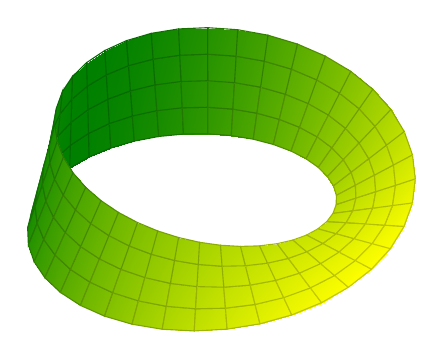
\begin{tikzpicture}
\begin{axis}[
    hide axis,
    view={40}{65}
]
\addplot3 [
    surf, shader = faceted interp,
    point meta = x,
    colormap/greenyellow,
    samples = 40,
    samples y = 5,
    z buffer = sort,
    domain = 0:360,
    y domain = -0.5:0.5,
    grid = none
] (
    {(1+0.5*y*cos(x/2)))*cos(x)},
    {(1+0.5*y*cos(x/2)))*sin(x)},
    {0.5*y*sin(x/2)});
\iffalse
\addplot3 [
    samples=50,
    domain=-145:180, % The domain needs to be adjusted manually, depending on the camera angle, unfortunately
    samples y=0,
    thick
] (
    {cos(x)},
    {sin(x)},
    {0});
\fi
\end{axis}
\end{tikzpicture}
\end{center}
	\fi
	There is a map from the M\"obius strip to the circle $S^1$, and the fibres of this map are isomorphic to $\mathbf{R}$. This gives a vector bundle over $S^1$ and it is not the trivial $\mathbf{R}\times S^1$: There is a ``twist'' in it.
\end{example}

One can define products on line bundles with tensor products of sheaves. Suppose that $(X,\mathscr{O}_X)$ is a ringed space. Let $\mathscr{F}$ and $\mathscr{G}$ be quasicoherent $\mathscr{O}_X$-modules. One defines the \defn{tensor product presheaf}\index{tensor product presheaf} by
\begin{align*}
	(\mathscr{F}\otimes^{\textrm{pre}}_{\mathscr{O}_X} \mathscr{G})(U) :=  \mathscr{F}(U) \tensor_{\mathscr{O}_X(U)}  \mathscr{G}(U)
\end{align*}
where $U\subset X$ is open. Now, one defines the \defn{tensor product sheaf}\index{tensor product sheaf} as the \index{sheafification}sheafification of the tensor product presheaf:
\begin{align*}
	\mathscr{F}\tensor_{\mathscr{O}_X} \mathscr{G} := (\mathscr{F}\tensor^{\textrm{pre}}_{\mathscr{O}_X}\mathscr{G})^\sharp.
\end{align*}

Note that the tensor product presheaf is not a sheaf even for line bundles over $\mathbf{P}^1$. Now, the tensor product of two $1$-dimensional vector spaces is $1$-dimensional, so one gets a line bundle from a product of two line bundles.

The \defn{Picard group}\index{Picard group} is the group of isomorphism classes of line bundles under $\tensor$. This combines the ideal class group, which is $\Pic(\Spec R)$, line bundles over a scheme, and the $1$-dimensional characters of a group.

\subsection{Invertible sheaves over the projective line.}
First, note my poor choice of notation. Sometimes I use the script-style $\mathscr{M}$ for modules over a ring or for quasicoherent modules. Two very different things. I will change.

\begin{definition}[Stacks project Definition 29.11.1]\label{}\text{}
A scheme morphism $\varphi : X\longrightarrow Y$ is \defn{affine}\index{affine morphism} if and only if the preimage of every affine open set of $Y$ is an affine open set of $X$.
\end{definition}

\begin{definition}[Stacks project Definition 27.6.1]\label{}\text{}
Let $S$ be a scheme. Let $\mathscr{M}$ be a quasicoherent $\mathscr{O}_S$-module. The \defn{vector bundle associated to $\mathscr{M}$}\index{vector bundle associated to a module} is
\begin{align*}
	\mathbf{V}(\mathscr{M}) := \underline{\Spec}_S(\Sym \mathscr{M}).
\end{align*}
This vector bundle has extra structure: There is a grading
\begin{align*}
	\pi_* \mathscr{O}_{\mathbf{V}(\mathscr{M})} = \bigoplus_{n\ge 0}\Sym ^n \mathscr{M}
\end{align*}
that makes $\pi_*\mathscr{O}_{\mathbf{V}(\mathscr{M})}$ a graded $\mathscr{O}_S$-algebra. One recovers $\mathscr{M}$ from the degree-$1$ part of this. 
\end{definition}

\begin{definition}[Stacks project Definition 27.6.2]\label{}\text{}
Let $S$ be a scheme. A \defn{vector bundle}\index{vector bundle over a scheme} $\pi:V\longrightarrow S$ over $S$ is an affine morphism of schemes such that $\pi_* \mathscr{O}_V$ is endowed with the structure of a graded $\mathscr{O}_S$-algebra 
\begin{align*}
	\pi_*\mathscr{O}_V = \bigoplus_{n\ge 0}\mathscr{M}_n
\end{align*}
such that $\mathscr{M}_0=\mathscr{O}_S$ and such that the maps
\begin{align*}
	\Sym^n \mathscr{M}_1\longrightarrow \mathscr{M}_n
\end{align*}
are isomorphisms for all $n\ge 0$. A  \defn{morphism of vector bundles over $S$}\index{morphism of vector bundles over a scheme} is a morphism $\varphi : V\longrightarrow V'$ such that the induced map
\begin{align*}
	\varphi^* : \pi_*' \mathscr{O}_{V'}\longrightarrow \pi_*\mathscr{O}_V
\end{align*}
is compatible with the given gradings.
\end{definition}

\begin{definition}[Stacks project Definition 15.117.1]\label{}\text{}
Let $A$ be a ring. An $A$-module $M$ is \defn{invertible}\index{invertible} if and only if the functor $(M\tensor_A \cdot) : \catn{Mod}(A) \longrightarrow \catn{Mod}(A)$ is an equivalence of categories.
\end{definition}


Recall \cref{thatinfamousdef} and \cref{this oneno}, too. Dr. Borcherds:
\begin{quote}
	\small The projective line over a field is, in algebraic geometry, something like the hydrogen atom in quantum mechanics. It's a very simple object which is complicated enough to exhibit some nontrivial phenomena and yet so easy [to work with] that you can calculate everything explicitly.
\end{quote}
So far, we have looked at quasicoherent sheaves on affine schemes. These are essentially the same as modules over rings.\footnote{``Talked about in a funny geometric language.''}
\begin{proposition}[Stacks project Lemma 17.24.5]\label{lemma_{17}above}
	Let $(X,\mathscr{O}_X)$ be a ringed space.
	\begin{enumerate}
		\item If $\mathscr{L}$ and $\mathscr{N}$ are invertible $\mathscr{O}_X$-modules, then so is $\mathscr{L}\tensor_{\mathscr{O}_X}\mathscr{N}$.
		\item If $\mathscr{L}$ is an invertible $\mathscr{O}_X$-module, then so is $\Hom_{\mathscr{O}_X}(\mathscr{L}, \mathscr{O}_X)$ and the \index{evaluation map}evaluation map $\mathscr{L}\tensor_{\mathscr{O}_X} \Hom_{\mathscr{O}_X}(\mathscr{L}, \mathscr{O}_X)\longrightarrow \mathscr{O}_X$ is an isomorphism.
	\end{enumerate}
\end{proposition}
 \begin{definition}[Stacks project Definition 17.24.9]\label{invertiblepic}\text{}
Let $(X,\mathscr{O}_X)$ be a ringed space. The \defn{Picard group}\index{Picard group} $\Pic X$ of $X$ is the abelian group whose elements are isomorphism classes of invertible $\mathscr{O}_X$-modules with addition given by the tensor product.
\end{definition}

\begin{problem}
	Find all invertible sheaves over $\mathbf{P}^1_K$. Invertible sheaves are, more or less, line bundles. Two invertible sheaves give an invertible sheaf via the tensor product in \cref{lemma_{17}above}. Therefore, given \cref{invertiblepic} or the line bundle definition, this is equivalent to determining $\Pic(\mathbf{P}^1_K)$.
\end{problem}

Let us guess by identifying the obvious line bundles. First, $\mathbf{P}^n_K =\mathbf{P}^n$ is the set of lines in $K^{n+1}$. Therefore, there is a map from the points of $\mathbf{P}^n$ to the $1$-dimensional vector spaces over $K$ given by
\begin{align*}
	(z_0:\cdots :z_n)\longmapsto \left\{ (\lambda z_0,\hdots,\lambda z_n):\lambda \in K \right\}. 
\end{align*}
Informally, this is a line bundle $\mathscr{L}$. One can consider $\mathscr{L}^{\tensor n} =: \mathscr{L}^n$ and $\mathscr{L}^* =: \mathscr{L}^{-1}$.\footnote{One takes the dual of a line bundle by taking the dual of every vector space.} Thus, one has $\mathscr{L}^n$ for $n\in\mathbf{Z}$. The claim is that these give all of the invertible sheaves over $\mathbf{P}^1_K$.\footnote{We shall consider $\mathbf{P}^n_K$ soon.}

Recall that one has $\mathbf{P}^1 = \mathbf{A}^1\cup \mathbf{A}^1$ via gluing. An invertible sheaf on $\mathbf{P}^1$ is given by an invertible sheaf over each copy of $\mathbf{A}^1$ and gluing them together on the intersection. First, one needs to determine the invertible sheaves on $\mathbf{A}^1$.

Since $\mathbf{A}^1$ is affine, sheaves correspond to modules over the coordinate ring $K[z]$. Since $K[z]$ is a principal ideal domain, all invertible sheaves are trivial: Invertible sheaves correspond to finitely-generated modules and finitely-generated modules over principal ideal domains are not invertible except for $K[z]$.

Now, one has modules $M_1=K[z_1]$ over $K[z_1]$ and $M_2 = K[z_2]$ over $K[z_2]$. One sets $z_2=z_1^{-1}$. The intersection here is $K[z_1,z_2]$, so one has module homomorphisms
\[
\begin{tikzcd}[sep = 3 em]
	K[z_1] \ar[r] & K[z_1,z_2]\\
		      &K[z_1,z_2]\ar[u,dashed]&K[z_2].\ar[l]
\end{tikzcd}
\]
One wants to determine the $K[z_1,z_2]$-module isomorphisms between the two copies of $K[z_1,z_2]$ above. These isomorphisms correspond to the units of $K[z_1,z_2]$, which are given by $\alpha z_1^n$ for $\alpha\in K^*$ and $n\in \mathbf{Z}$. One can multiply by the units of $K[z_1]$ and $K[z_2]$ without changing the isomorphism classes, so one can assert that $\alpha = 1$. Fix $n\in \mathbf{Z}$. One sees that
\[
\begin{tikzcd}[sep = 3 em]
	K[z_1]\ar[r]& K[z_1,z_2] \ar[d, "1\longmapsto z_2^n", swap] \\
	&K[z_1,z_2] \ar[u,"1\longmapsto z_1^n",xshift = 1 em, swap] &K[z_2]\ar[l] 
\end{tikzcd}
\]
gives the gluing of two modules. This gives a sheaf over $\mathbf{P}^1$ denoted $\mathscr{O}(n)$.

Thus, every invertible sheaf over $\mathbf{P}^1$ is of the form $\mathscr{O}(n)$. The claim is that these are distinct. Let us consider the global sections $\Gamma(\mathscr{O}(n))$. To choose a global section of $\mathscr{O}(n)$, one must choose an element $\varphi(z_1) \in K[z_1]$ and $\psi(z_2)\in K[z_2]$ and glue them together by $z_2^n\varphi(z_1) =\psi(z_2)$. That is, $z^n\varphi(z^{-1}) = \psi (z)$. Therefore, $\deg \varphi \le n$, and the dimension of the vector space of such polynomials is $n+1$ for nonnegative $n$ and $0$ otherwise. That is,
\begin{align*}
	\dim \Gamma(\mathscr{O}(n)) = 
	\begin{cases}
		n+1&n\ge 0\\
		0 &\textrm{otherwise.}
	\end{cases}
\end{align*}
Therefore, the $\mathscr{O}(n)$s are distinct for $n\ge 0$. One can see that this holds in general by noting that
\begin{align*}
	\mathscr{O}(m) \tensor \mathscr{O}(n) \isomto \mathscr{O}(m+n)\textrm{:}
\end{align*}
If one glues two modules by multiplying by $z_2^m$ and glues two other modules by multiplying by $z_2^n$ and then takes the tensor product, one glues by multiplying by $z_2^{m+n}$. Also, one notes that the dual of $\mathscr{O}(m)$ is $\mathscr{O}(-m)$, which follows in much the same way. Either way, all of the $\mathscr{O}(n)$s are distinct. 

Therefore, 
\begin{align*}
	\Pic (\mathbf{P}^1_K) \isomto \mathbf{Z}.
\end{align*}

One notes that $\Gamma(\mathscr{O}(n))$ is finite-dimensional over $K$. The global sections of sheaves over projective spaces tends to be much smaller than that over affine spaces. This is a special case of a very general theorem that states that the cohomology of coherent sheaves over projective varieties is finite-dimensional.\footnote{See Serre and Cartan's ``Un th\'eor\`eme de finitude concernant les vari\'et\'es analytiques compactes,'' 1953.}

Recall that 
\begin{align*}
	\mathscr{F}\otimes^{\textrm{pre}}_{\mathscr{O}_X} \mathscr{G},
\end{align*}
in which one defines the tensor product in the most natural way, does not give a sheaf necessarily. One sees that
\begin{align*}
	\dim( \Gamma(\mathscr{O}(-1) \otimes^{\textrm{pre}}_{\mathscr{O}_X} \mathscr{O}(1) )) = 1
\end{align*}
and 
\begin{align*}
	\dim(\Gamma\mathscr{O}(-1) \tensor \Gamma\mathscr{O}(1) ) = 0.
\end{align*}
Thus, 
\begin{align*}
	\Gamma(\mathscr{O}(-1) \otimes^{\textrm{pre}}_{\mathscr{O}_X} \mathscr{O}(1) ) \ne \Gamma\mathscr{O}(-1) \tensor \Gamma\mathscr{O}(1),
\end{align*}
and
\begin{align*}
	(\mathscr{O}(-1) \otimes^{\textrm{pre}}_{\mathscr{O}_X} \mathscr{O}(1))(\mathbf{P}^1) \ne \mathscr{O}(-1) (\mathbf{P}^1) \tensor \mathscr{O}(1) (\mathbf{P}^1).
\end{align*}
This is a nice counterexample.

Let us look at the morphisms $\mathscr{O}(m) \longrightarrow \mathscr{O}(n)$. These are isomorphic to morphisms from $\mathscr{O}(0)$ to $\mathscr{O}(n-m)$ via $\cdot\tensor \mathscr{O}(-m)$. This is $\Gamma(\mathscr{O}(n-m))$ of dimension $n-m+1$ for $n\ge m$ and of dimension $0$ otherwise.

\begin{remark}
	There is a more straightforward way to describe morphisms at which we shall look later using graded modules over graded rings.
\end{remark}

Consider the exact sequence
\[
\begin{tikzcd}
	0\ar[r] &\mathscr{O}(-1) \ar[r]& \mathscr{O}(0) \oplus \mathscr{O}(0)\ar[r,"1\oplus z"] & \mathscr{O}(1)\ar[r]&0.
\end{tikzcd}
\]
The third arrow is surjective since the morphism from the first $\mathscr{O}(0)$ to the first $\mathbf{A}^1$ is surjective and the morphism from the second $\mathscr{O}(0)$ to the second $\mathbf{A}^1$ is surjective, so it is surjective on the fibres. One does not need to know how the kernel of the third arrow is $\mathscr{O}(-1)$. With $\cdot\tensor \mathscr{O}(-1)$, which preserves exactness on invertible sheaves,\footnote{This preserves exactness on invertible sheaves since invertible sheaves look like free sheaves locally and exactness is a local property. It does not in general.}
\[
\begin{tikzcd}
	0\ar[r]&\mathscr{O}(-2) \ar[r] &\mathscr{O}(-1) \oplus \mathscr{O}(-1) \ar[r] & \mathscr{O}(0) \ar[r] &0.
\end{tikzcd}
\]
There are no nonzero morphisms from $\mathscr{O}(0)$ to $\mathscr{O}(-1)$, so this is non-split. Now, $\mathscr{O}(0)$ is the sheaf of coordinate functions over $\mathbf{P}^1$. Over any ring $R$,
\[
\begin{tikzcd}
	0\ar[r]&A\ar[r]&B\ar[r]&R\ar[r]&0
\end{tikzcd}
\]
splits. So, over any affine scheme $\Spec R$,
\[
\begin{tikzcd}
	0\ar[r]&\mathscr{M}\ar[r]&\mathscr{N}\ar[r]&\mathscr{O}_{\Spec R}\ar[r]&0
\end{tikzcd}
\]
splits. The sheaf of coordinate functions is always a ``projective module'': Free sheaves are projective over affine schemes. However, in the demonstration above, one has a free sheaf that is not projective over projective space.
\begin{quote}
	\small Free sheaves need not be projective!
\end{quote}
This is not the case in differential geometry but it is in algebraic geometry.

Now, consider 
\[
\begin{tikzcd}
	0\ar[r]&\mathscr{O}(-2) \ar[r] &\mathscr{O}(-1) \oplus \mathscr{O}(-1) \ar[r] & \mathscr{O}(0) \ar[r] &0.
\end{tikzcd}
\]
Taking global sections,
\[
\begin{tikzcd}
	0\ar[r]&\Gamma(\mathscr{O}(-2)) \ar[r] &\Gamma (\mathscr{O}(-1) \oplus \mathscr{O}(-1)) \ar[r] & \Gamma(\mathscr{O}(0)) \ar[r] &0
\end{tikzcd}
\]
is not exact: The only problem is that the last arrow is not surjective. Everything else is trivial. Taking global sections preserves left exactness. More precisely, if
\[
\begin{tikzcd}
	0\ar[r]&\mathscr{A}\ar[r]&\mathscr{B}\ar[r]&\mathscr{C}\ar[r]&0
\end{tikzcd}
\]
is an exact sequence of quasicoherent sheaves,
\[
\begin{tikzcd}
	0\ar[r] &\Gamma(\mathscr{A}) \ar[r]& \Gamma(\mathscr{B})\ar[r]&\Gamma(\mathscr{C}) \ar[r]&\HH^1(\mathscr{A}) \ar[r]&\HH^1(\mathscr{B}) \ar[r]&\HH^1(\mathscr{C})\ar[d]\\&&&&&\cdots&\HH^2(\mathscr{A}) \ar[l]
\end{tikzcd}
\]
is exact.

There are three main things that are different for schemes over non-affine spaces:
\begin{enumerate}
	\item Tensor products do not behave in the natural way;
	\item Free sheaves are not necessarily projective;
	\item The map got by taking global sections of a surjective map of sheaves does not need to be surjective.
\end{enumerate}

\subsection{The functors \texorpdfstring{$f^*$}{f*} and \texorpdfstring{$f_*$}{f*}. Extension by zero.}
Suppose that $f:X\longrightarrow Y$ is a morphism of schemes. If $\mathscr{F}$ is a quasicoherent sheaf on $Y$, then $f^*(\mathscr{F})$ is a quasicoherent sheaf on $X$. Similarly, if $\mathscr{G}$ is a quasicoherent sheaf on $X$, $f_*(\mathscr{G})$ is a quasicoherent sheaf on $Y$. The functor $f^*$ is left adjoint to $f_*$. Let us look at these functors and consider the affine case first. 

Suppose that $A \longleftarrow B$ is a ring homomorphism. Then, if $M$ is an $A$-module, it is a $B$-module via the functor $g: \catn{Mod}(A) \longrightarrow \catn{Mod}(B)$ given by $M\longmapsto M$. If $N$ is a $B$-module, it is not an $A$-module; however, $N\tensor_B A$ is an $A$-module. Consider the functor $\tilde g = \cdot\tensor_B A: \catn{Mod}(B) \longrightarrow \catn{Mod}(A)$ given by $N\longmapsto N\tensor_B A$. This map $\tilde g$ is left adjoint to the map $g$. 

Rather clearly, $g$ preserves exactness. However, without thinking, one has only the preservation of right exactness for $\tilde g$. Now, $\cdot \tensor_B A$ preserves exactness if $A$ is a flat\index{flat module} $B$-module.\footnote{By definition.}

Now, write $X :=\Spec A$ and $Y:=\Spec B$. Consider the morphism of schemes $f:X\longrightarrow Y$. One can pull back a sheaf $\mathscr{F}$ on $Y$ to a sheaf $f^{-1}(\mathscr{F})\tensor_{f^{-1}(\mathscr{O}_Y)} \mathscr{O}_X$ on $X$. One can make a sheaf $\mathscr{G}$ on $X$ a sheaf $f_*(\mathscr{G})$ on $Y$. Now, define $f^* :\catn{QCoh}(\mathscr{O}_Y)\longrightarrow \catn{QCoh}(\mathscr{O}_X)$ 
\begin{align*}
	f^*(\mathscr{F}) := f^{-1}(\mathscr{F}) \tensor_{f^{-1}(\mathscr{O}_Y)} \mathscr{O}_X
\end{align*}
and $f_* : \catn{QCoh}(\mathscr{O}_X)\longrightarrow \catn{QCoh}(\mathscr{O}_Y)$ as in \cref{functorsp_1}. Then, $f^*$ and $f_*$ are adjoint.\footnote{Where $f^*$ is left adjoint to $f_*$.}

For affine schemes, $f_*$ is exact and $f^*$ is right exact (and exact if flatness holds).\footnote{All of this is so easy because the category of affine schemes is equivalent to the opposite category of rings.}

Consider a morphism of schemes $f:X\longrightarrow Y$. For a sheaf $\mathscr{F}$ on $Y$, one gets a sheaf $f^*(\mathscr{F})$ on $X$. For a sheaf $\mathscr{G}$ on $X$, one gets a sheaf $f_*(\mathscr{G})$ on $Y$. One sees that adjointness still holds. The functor $f^*$ is defined in the same way as above, and $f^*(\mathscr{F})$ looks like $N\tensor_B A$ locally.

Now, $f^*$ is left adjoint to $f_*$, so $f^*$ is right exact.\footnote{Left adjoints are right exact.} The functor $f^*$ is exact if some flatness condition holds. Similarly, $f_*$ is left exact. However, $f_*$ is not exact in general. We have seen this: Consider $f:\mathbf{P}^1_K\longrightarrow \Spec K$. One sees that taking $f_*$ is the same as taking global sections. Now, 
\[
\begin{tikzcd}
	\mathscr{O}(-1) \oplus \mathscr{O}(-1)\ar[r]& \mathscr{O}(0) \ar[r] & 0
\end{tikzcd}
\]
is exact, but, taking global sections, one has
\[
\begin{tikzcd}
 f_*(\mathscr{O}(-1) \oplus \mathscr{O}(-1))\ar[r]& f_*(\mathscr{O}(0)) \ar[r] & f_*(0)
\end{tikzcd}
\]
and the second arrow is not surjective.

Given an exact sequence
\[
\begin{tikzcd}
	0\ar[r]&\mathscr{A}\ar[r]&\mathscr{B}\ar[r]&\mathscr{C}\ar[r]&0,
\end{tikzcd}
\]
one gets a long exact sequence
\[
\begin{tikzcd}
	 0\ar[r] &f_*(\mathscr{A}) \ar[r]& f_*(\mathscr{B})\ar[r]&f_*(\mathscr{C}) \ar[r]&\mathscr{R}^1f_*(\mathscr{A}) \ar[r]&\mathscr{R}^1f_*(\mathscr{B}) \ar[d]\\&&&\cdots&\mathscr{R}^2f_*(\mathscr{A}) \ar[l]&\mathscr{R}^1f_*(\mathscr{C})\ar[l]
\end{tikzcd}
\]
where $\mathscr{R}^nf_*$ is the $n$th \index{right derived functor}right derived functor of $f_*$. 

Suppose that $f:U\longrightarrow X$ is an open immersion. Then, in addition to the functor $f_*$, one has the functor $f_!$ which is \defn{extension by zero}\index{extension by zero}.\footnote{``$f$ sub shriek.''} One can think of a sheaf $\mathscr{F}$ on $U$ as an \'etale map from the \'etale space of $\mathscr{F}$ $\Et(\mathscr{F})$ to $U$.\footnote{Recall that an \'etale map is just a local homeomorphism.} Since $f$ is an open immersion, the map got by the composition of this \'etale map and $f$ gives the \'etale map $\Et(f_!(\mathscr{G}))\longrightarrow X$.\footnote{The stalk of $f_!(\mathscr{F})$ is $0$ if the point is not in the image of $U$ and is the stalk of $\mathscr{F}$ if the point is in the image of $U$.}

Suppose that $\mathscr{Q}$ is a quasicoherent sheaf. Then, $f_!(\mathscr{Q})$ is not quasicoherent in general.

\begin{example}[ ]\label{}\text{}
Consider $f:\Spec K\longrightarrow \Spec R$ where $R$ is a discrete valuation ring. Consider the sheaf $\mathscr{K}$ corresponding to the module $K$. Now, $f_*(\mathscr{K}) =\mathscr{K}$. However, the stalk of $f_!(\mathscr{K}) $ at the closed point is $0$, so $f_!(\mathscr{K})$ has no global sections other than $0$, so it is not quasicoherent.\footnote{Any quasicoherent sheaf is determined by its module of global sections.} However, $f_!(\mathscr{K})$ is a $\mathscr{O}_{\Spec R}$-module.
\end{example}

The functor $f_!$ is left adjoint to $f^*=f^{-1}$ and $f_*$ is right adjoint to it.

\begin{definition}[Stacks project Definition 59.70.1]\label{}\text{}
Let $j:U\longrightarrow X$ be an \'etale morphism of schemes.
\begin{enumerate}
	\item The restriction functor $j^{-1} :\catn{Sh}(X\textsubscript{\'etale})  \longrightarrow \catn{Sh}(U\textsubscript{\'etale})$ has a left adjoint $j_!^{\textrm{Sh}} : \catn{Sh}(U\textsubscript{\'etale}) \longrightarrow \catn{Sh}(X\textsubscript{\'etale})$.
	\item The restriction functor $j^{-1} : \catn{Ab}(X\textsubscript{\'etale}) \longrightarrow \catn{Ab}(U\textsubscript{\'etale})$ has a left adjoint which is denoted $j_! : \catn{Ab}(U\textsubscript{\'etale}) \longrightarrow \catn{Ab}(X\textsubscript{\'etale})$ and called \defn{extension by zero}\index{extension by zero}.
	\item Let $\Lambda$ be a ring. The restriction functor $j^{-1} : \catn{Mod}(X\textsubscript{\'etale}, \Lambda)  \longrightarrow \catn{Mod}(U\textsubscript{\'etale}, \Lambda)$ has a left adjoint which is denoted $j_! : \catn{Mod}(U\textsubscript{\'etale}, \Lambda) \longrightarrow \catn{Mod}(X\textsubscript{\'etale}, \Lambda)$ and called \defn{extension by zero}\index{extension by zero}.
\end{enumerate}
\end{definition}

\subsection{Coherent sheaves.}
\begin{definition}[Stacks project Definition 17.12.1]\label{cohs}\text{}
Let $(X,\mathscr{O}_X)$ be a ringed space. Let $\mathscr{F}$ be a sheaf of $\mathscr{O}_X$-modules. The sheaf $\mathscr{F}$ is a \defn{coherent $\mathscr{O}_X$-module}\index{coherent sheaf} if and only if $\mathscr{F}$ is of finite type and, for every open $U\subset X$ and every finite collection $\{s_1,\hdots,s_n\}\subset \mathscr{F}(U)$, the kernel of the associated map
\begin{align*}
	\bigoplus_{i=1,\hdots, n}\mathscr{O}_U \longrightarrow \mathscr{F}\big |_U
\end{align*}
is of finite type.

One denotes the category of coherent $\mathscr{O}_X$-modules $\catn{Coh}(\mathscr{O}_X)$.
\end{definition}

The relationship between coherent sheaves and sheaves is similar to the relationship between finite-dimensional vector spaces and vector spaces.

First, let us consider the case of modules over a ring. It might make sense for a coherent module to be a finitely generated module. However, while this works well for Noetherian rings, it doesn't work in general: The kernel of a homomorphism of finitely generated modules does not need to be finitely generated.

\begin{example}[ ]\label{}\text{}
Consider $R = K[z_1,z_2,\hdots]$. The kernel of $R\longrightarrow R$ given by $z_i \longmapsto 0$ is $(z_1,z_2,\hdots)$ which is not finitely generated.
\end{example}

This raises the problem of finding an abelian category of modules.\footnote{That is, one with kernels, cokernels, etc.}

\begin{definition}[ ]\label{}\text{}
Let $A$ be a ring. Let $M$ be an $A$-module. Then, $M$ is \defn{coherent}\index{coherent module} if and only if $M$ is finitely generated and the kernel of any homomorphism $R^n\longrightarrow M$ is finitely generated.
\end{definition}

\begin{remark}
	If $M$ is coherent, then $M$ is finitely presented.
\end{remark}

The category of coherent modules forms an abelian category.

 \begin{definition}[ ]\label{}\text{}
Let $A$ be a ring. Then, $A$ is \defn{coherent}\index{coherent ring} if and only if $A$ is a coherent $A$-module.
\end{definition}

Over coherent rings, coherent modules are the same as finitely presented modules. Over Noetherian rings, coherent modules are the same as finitely generated modules.

\begin{example}[ ]\label{}\text{}
The ring $K[z_1,z_2,\hdots]$ is coherent but not Noetherian. 

The ring $K[z_1,z_2,\hdots]/(z_1z_2,z_1z_3,\hdots)$ is not coherent, for the kernel of $R\longrightarrow R$ given by $1\longmapsto z_1$ is $(z_2,\hdots)$ which is not finitely generated. This ring is a finitely presented module that is not coherent.
\end{example}

\index{coherent sheaf}Coherent sheaves were introduced for complex analytic manifolds. Serre and Cartan studied complex analytic manifolds with sheaves and Serre introduced sheaves to algebraic geometry after this work with analytic manifolds. 

The sheaf of holomorphic functions on a complex analytic manifold $X$ gives rings that are not Noetherian. The ring of holomorphic functions on $\mathbf{C}^1$ is not Noetherian: The ideal of all functions that vanish on all but finitely many integers is not finitely generated. Kiyoshi Oka showed that the sheaf of holomorphic functions on a complex analytic manifold is coherent.\footnote{See ``Sur les fonctions analytiques de plusieurs variables. VII. Sur quelques notions arithmétiques,'' 1950. This result is called the ``Oka coherence theorem.''}\index{Oka coherence theorem}

That rings of holomorphic functions are not Noetherian is subtle: One has the inclusions
\begin{align*}
	\mathbf{C}[z] \subset \textrm{holomorphic functions} \subset \mathbf{C}[\![z]\!].
\end{align*}
The rings $\mathbf{C}[z]$ and $\mathbf{C}[\![z]\!]$ are Noetherian.

Recall \cref{cohs}. The ringed space of interest here was $(\mathbf{C}^n, \mathscr{O}_{\mathbf{C}^n})$ where $\mathscr{O}_{\mathbf{C}^n}$ is the sheaf of holomorphic functions that assigns an open set $U$ to the ring of holomorphic functions on $U$.

Suppose that $\mathscr{O}_X$ is coherent. The sheaf $\mathscr{F}$ is coherent if and only if there exists an exact sequence
\[
\begin{tikzcd}
	\displaystyle\bigoplus_{i=1,\hdots,m} \mathscr{O}_X\ar[r]& \displaystyle\bigoplus_{i=1,\hdots,n} \mathscr{O}_X \ar[r]&\mathscr{F}\ar[r]&0.
\end{tikzcd}
\]
This is the sheaf-theoretic analogue of a module being of finite presentation.

Now, $\mathscr{F}$ is \index{quasicoherent sheaf}quasicoherent if and only if there exists an exact sequence
\[
\begin{tikzcd}
	\displaystyle \bigoplus_{}\mathscr{O}_X \ar[r] & \displaystyle \bigoplus_{}\mathscr{O}_X\ar[r]&\mathscr{F}\ar[r]&0.
\end{tikzcd}
\]
Notice that this notion of quasicoherence is vacuous for modules.

For affine schemes, this is equivalent to the condition that $\mathscr{F}$ is of the form $\mathscr{M}$ locally.\footnote{Before, I would write ``of the form $\overline{\mathscr{M}}$.''}

\begin{remark}
	Hartshorne defines ``coherent'' as ``quasicoherent and of finite type.'' This works for Noetherian schemes, but it goes wrong for schemes in general.
\end{remark}

The category $\catn{Coh}(\mathscr{O}_X)$ is abelian.

\begin{example}[ ]\label{}\text{}
The sheaves $\mathscr{O}(n)$ over $\mathbf{P}^1_K$ are coherent.
\end{example}

\begin{problem}
	Given a coherent (resp. quasicoherent) sheaf $\mathscr{F}$, are $f^*(\mathscr{F})$ and $f_*(\mathscr{F})$ coherent (resp. quasicoherent)?
\end{problem}

Suppose that $f:X\longrightarrow Y$ is a morphism of schemes. Then, $f^*$ preserves quasicoherence and $f^*$ preserves coherence if $X$ is coherent.

If $\mathscr{Q}$ is quasicoherent, $f_*(\mathscr{Q})$ is usually quasicoherent.
\begin{example}[$f_*$ does not preserve quasicoherence]\label{}\text{}
Suppose that $X$ is a union of infinitely many copies of $\Spec R$ where $R$ is a discrete valuation ring. Suppose that $Y=\Spec R$. Let $\mathscr{F}$ be a copy of $\mathscr{R}$, the sheaf associated to $R$, over each $\Spec R$. Now, $\mathscr{F}$ has two nonempty open sets; one sees that
\begin{align*}
	f_*(\mathscr{F})(\Spec K) &= \prod_{ \mathbf{N}} K;\\
	f_*(\mathscr{F}) (\Spec R) &= \prod_{ \mathbf{N}} R.
\end{align*}
However,
\begin{align*}
	\left( \prod_{\mathbf{N}} R \right) \tensor_R K \ne \prod_{\mathbf{N}}K.
\end{align*}
One can consider the element $(1/2,1/4,1/8,\hdots)$ where $R=\mathbf{Z}_{(2)}$ and $K=\mathbf{Q}$, which is in the second thing but not the first thing. The first thing has bounded denominators and the second thing does not need to have bounded denominators.
\end{example}

\begin{theorem}[ ]\label{}\index{}\text{}
Suppose that $f:X\longrightarrow Y$ is a quasicompact and quasiseparated morphism of schemes. Then, $f_*$ preserves quasicoherence.
\end{theorem}

\begin{proof}
Stacks project Lemma 26.24.1.
\end{proof}

Now, while
\begin{align*}
	f_*(\mathscr{F}\oplus \mathscr{G}) = f_*(\mathscr{F}) \oplus  f_*(\mathscr{G}),
\end{align*}
unfortunately,
\begin{align*}
	f_* \left( \bigoplus_{i}\mathscr{F}_i \right)\ne \bigoplus_{i}f_*(\mathscr{F}_i). 
\end{align*}
Quasicompactness and quasiseparatedness allow one to exchange $f_*$ and direct sums.

One asks:
\begin{quote}
	\small Does $f_*$ preserve coherence?
\end{quote}
Dr. Borcherds answers:
\begin{quote}
	\small The answer is a big, resounding ``no''!
\end{quote}
Consider the morphism $f:\mathbf{A}^1\longrightarrow \Spec K$. Take $\mathscr{F} $ to be the sheaf of coordinate functions $\widetilde{K[z]}$. This sheaf is coherent, but $f_*(\mathscr{F})$ is $\widetilde{K[z]}$ over $\Spec K$, which corresponds to the $K$-module $K[z]$ which is not finitely generated as a $K$-module. 

Suppose that $f:X\longrightarrow Y$ is a proper morphism of schemes where $Y$ is Noetherian. Then, $f_*$ preserves coherence.\footnote{Stacks project Proposition 30.19.1 is a generalization of this to right derived functors.} We have seen this: Consider $f:\mathbf{P}^1_K\longrightarrow \Spec K$. Then, $f_*(\mathscr{O}(n))$ is a finite-dimensional vector space over $K$, which corresponds to a coherent sheaf over $\Spec K$.

\subsection{The line bundles \texorpdfstring{$\mathscr O(n)$}{O(n)} on projective space.}

One wants to construct examples of coherent sheaves on projective space. We concocted examples on $\mathbf{P}^1$ by gluing; however, gluing isn't very elegant, and things can get quite convoluted. 

For affine schemes $\Spec A$, quasicoherent sheaves correspond to $A$-modules.\footnote{Via an equivalence of categories.}
For projective schemes of the form $\Proj A$ where $A$ is a graded ring, quasicoherent modules subtly correspond to graded $A$-modules.\footnote{See \cref{ega552}.} Let us explore this correspondence.

First, recall that the points of $\Proj A$ consist of the graded prime ideals of $A$ that do not contain
\begin{align*}
	\bigoplus_{i>0}A_i,
\end{align*}
the basis of open sets is given by $\{U(f):f\in A\}$ where $U(f)$ consists of the prime ideals that do not contain $f$,\footnote{One thinks of this as ``the points where $f$ is nonzero.''} and the ring of regular functions is given by
\begin{align*}
	\mathscr{O}(U(f)) := A[f^{-1}]^0.
\end{align*}
\begin{example}[ ]\label{}\text{}
Let $A = K[z_1,\hdots,z_n]$. The closed points of $\Proj A$ correspond to points $(z_0:\cdots:z_n)\sim (\lambda z_0:\cdots:\lambda z_n)$ for $\lambda\ne 0$. The open sets $U(z_i)$ are given by affine space
\begin{align*}
	\left\{ (z_0,\hdots,z_n) : \textrm{$1$ in the $i$th position} \right\}. 
\end{align*}
Finally,
\begin{align*}
	\mathscr{O}(U(z_i)) &= K[z_0,\hdots, z_n][z_i^{-1}]^0\\
			    &= K \left[ \frac{z_0}{z_i},\hdots, \frac{z_n}{z_i} \right]^0. 
\end{align*}
\end{example}

Suppose that $M$ is a graded $A$-module. One wants to define a sheaf $\mathscr{M}$ on $\Proj A$. For the graded $A$-module $A$, one defines this sheaf by
\begin{align*}
	\mathscr{O}(U(f)) := A[f^{-1}]^0.
\end{align*}
Thus, one defines
\begin{align*}
	\mathscr{M}(U(f)) := M[f^{-1}]^0.
\end{align*}
Showing that this defines a sheaf is similar to showing that $\Proj A$ is a scheme.
\begin{quote}
	\small [This definition] is somehow part of Grothendieck's philosophy that the points of a scheme are . . . not terribly important. What is really important is the open sets together with which open sets cover the others. It is actually the basis for something called a Grothendieck topology because Grothendieck realized you could define sheaves by ignoring the points completely and just working with the open sets. You just need to define something for each open set and check some property holds whenever open sets cover other open sets. Grothendieck . . . axiomatized this and came up with the idea of a Grothendieck topology, which turns out to be really useful for defining things like \'etale cohomology where you replace open sets with something a little bit more complicated than open sets and you can still define sheaves on those.\index{Grothendieck topology}
\end{quote}

\begin{example}[ ]\label{}\text{}
Let $A = K[z_0,\hdots,z_r]$. Then, $\Proj A = \mathbf{P}^r_K$. A variety $V\subset \mathbf{P}^r_K$ corresponds to a graded ideal $I$. Take $M:=A/I$. Then, $\mathscr{M}$ is sort of a sheaf with support on $V$.

Note that the sheaf $\mathscr{I}$ corresponding to $I$ tends to be uninteresting. For example, if $V$ is the zero locus of $f$, then $I=fA\isomto A$.
\end{example}

One can shift the grading on graded modules. If 
\begin{align*}
	M = \bigoplus_{i\ge 0}M_i,
\end{align*}
then
\begin{align*}
	M(n) = \bigoplus_{i\ge 0}M (n)_i :=  \bigoplus_{i\ge 0} M_{n+i}.
\end{align*}
Now, let us determine $\widetilde{A(n)}$.\footnote{That is, the sheaf given by $A(n)$.} First,
\begin{align*}
	\widetilde{A(0) } = \tilde A = \mathscr{O}_{\mathbf{P}^r_K}.
\end{align*}
Now, $\widetilde {A(n)} (U(z_i))$ is given by the degree-$0$ elements of $K[z_0,\hdots,z_r][z_i^{-1}]$ grading-shifted by $n$. Now, this shifting seems to make no difference, since $z_i$ is an isomorphism from the degree-$m$ piece of $K[z_0,\hdots,z_r][z_i^{-1}]$ to the degree-$(m+1) $ piece. Therefore, $\widetilde{A(n)}$ is isomorphic to $\widetilde{A(0)}$ over every $U(z_i)$.

Thus, $\widetilde{A(n)}$ is locally isomorphic to $\tilde A$, so $\widetilde{A(n)}$ is an \index{invertible sheaf}invertible sheaf.\footnote{Or a line bundle.} One distinguishes $\widetilde{A(n)}$ from $\tilde A$ by computing global sections. Take a section over $U(f_i)$ that is a degree-$n$ element of $K[z_0,\hdots,z_r][z_i^{-1}]$ and glue it over a section of $U(f_j)$ that is a degree-$n$ element of $K[z_0,\hdots,z_r][z_j^{-1}]$ for all $j$. These sections must be the same over $K[z_0,\hdots,z_r][z_i^{-1},z_j^{-1}]$, so the degree-$n$ element must be a polynomial. Thus, one sees that $\Gamma(\widetilde{A(n)})$ is given by the homogeneous degree-$n$ polynomials in $K[z_0,\hdots,z_r]$ for $r\ge 1$. Now,
\begin{center}
\begin{tabular}{lccccc}
     & $\mathbf{P}^0$&$\mathbf{P}^1$&$\mathbf{P}^2$& $\mathbf{P}^3$&$\mathbf{P}^4$\\
    \midrule
	$\dim \Gamma (\widetilde{A(-2)})$ &$1$&$0$&$0$&$0$&$0$\\
	$\dim \Gamma (\widetilde{A(-1)})$&$1$&$0$&$0$&$0$&$0$\\
	$\dim \Gamma (\widetilde{A(0)})$&$1$&$1$&$1$&$1$&$1$\\
	$\dim \Gamma (\widetilde{A(1)})$&$1$&$2$&$3$&$4$&$5$\\
	$\dim \Gamma (\widetilde{A(2)})$&$1$&$3$&$6$&$10$&$15$
\end{tabular}
\end{center}
One beholds Pascal's triangle here and one sees that many of these are distinct. 
Now, note the following properties:
\begin{align*}
	\tilde M\tensor \tilde N &\isomto \widetilde{M\tensor N};\\
	\widetilde{M(n)} &\isomto \tilde M (n);\\
	\widetilde {M (n) } &\isomto \tilde M \tensor \widetilde{A(n)}.
\end{align*}
Therefore,
\begin{align*}
	\widetilde{A (m)} \tensor \widetilde {A (n)} \isomto \widetilde{A (m+n)}
\end{align*}
and all of the line bundles $\widetilde{A(n)}$ are distinct.

\begin{problem}
	Can one recover $M$ from $\tilde M$?\footnote{That is, from $\mathscr{M}$?}
\end{problem}

While one can do this for affine schemes,\footnote{Where one considers the global sections.} one cannot do this in general: If $M=K$, then $\tilde M = 0$. However, this is the only problem arises, and it shows up when $M$ is finite dimensional as a $K$--vector space.

Suppose that $\mathscr{F}$ is a sheaf over $\mathbf{P}^r_K$. Then, define 
\begin{align*}
	\mathscr{F}(n):=  \mathscr{F}\tensor \underbrace{\mathscr{O}(n).}_{\widetilde{A(n)}}
\end{align*}
Now, $\Gamma(\mathscr{F})$ does not give very much information, so one considers the ``graded global sections'' of $\mathscr{F}$:
\begin{align*}
	\Gamma_*(\mathscr{F}) := \bigoplus_{n\in\mathbf{Z}} \Gamma(\mathscr{F}(n)).
\end{align*}
For example,
\begin{align*}
	\Gamma_*(\mathscr{O}) = K[z_0,\hdots, z_r]
\end{align*}
since
\begin{align*}
	\Gamma_0(\mathscr{O}) &= K;\\
	\Gamma_1(\mathscr{O}) &= \langle z_0,\hdots, z_r\rangle;\\
	\Gamma_2(\mathscr{O}) &= \langle z_iz_j\rangle;
\end{align*}
etc.
Further, $\Gamma_*(\mathscr{F})$ is a graded module over $\Gamma_*(\mathscr{O}) = K[z_0,\hdots, z_r]$.\footnote{Since there is a map $\mathscr{O}(m)\tensor  \mathscr{F}(n) \longrightarrow \mathscr{F}(m+n)$.}

One has a correspondence between finitely generated graded modules over $K[z_0,\hdots,z_r]$ and coherent sheaves on $\mathbf{P}^r_K$. The functor $\Gamma_*$ takes coherent sheaves to graded modules and $M\longmapsto \tilde M$ takes graded modules to coherent sheaves. These are not inverses of each other: We saw that $\Gamma_*(\tilde M)$ does not need to be isomorphic to $M$. However, 
\begin{align*}
	\widetilde{\Gamma_*(\mathscr{F}) } \isomto \mathscr{F}.
\end{align*}

\subsection{Vector bundles on the projective line.}
Note a notational shift: We shall use $\tilde M$ to refer to the sheaf associated to a module $M$, not $\mathscr M$, because we cannot ``scriptify'' everything: For example, $A(n)$. Furthermore, sometimes, it is difficult to determine automatically what letter is being written. 

Formally recall:

\begin{definition}[Stacks project Definition 27.10.1]
Let $S$ be a graded ring. Let $X=\Proj S$.
\begin{enumerate}
	\item One defines $\mathscr{O}_X(n)=\mathscr{O}(n) := \widetilde{S(n)}$. This is called the \defn{$n$th twist of the structure sheaf}\index{twist of a sheaf} of $\Proj S$.
	\item For any sheaf of $\mathscr{O}_X$ modules $\mathscr{F}$, one sets
	\[
		\mathscr{F}(n):= \mathscr{F} \tensor_{\mathscr{O}_X} \mathscr{O}_X(n).
	\]	
\end{enumerate}

\end{definition}

Last time, we investigated the line bundles/invertible sheaves $\mathscr{O}(n)$. These are locally free. This is motivates one to classify locally free sheaves on a scheme $X$. This is difficult if $\dim X>1$ and if the rank of the sheaf is greater than $1$.

\begin{definition}[Stacks project Definition 17.14.1]\label{}\text{}
Let $(X,\mathscr{O}_X)$ be a ringed space. Let $\mathscr{F}$ be a sheaf of $\mathscr{O}_X$-modules.
\begin{enumerate}
	\item One says that $\mathscr{F}$ is \defn{locally free}\index{locally free sheaf} if and only if, for every point $x\in X$, there exist a set $I$ and an open neighbourhood $U$ of $x$ such that $\mathscr{F}\big|_U$ is isomorphic to 
		\begin{align*}
			\bigoplus_{i\in I}\mathscr{O}_X\big|_U 
		\end{align*}
		as an $\mathscr{O}_X\big|_U$-module.
	\item One says that $\mathscr{F}$ is \defn{finite locally free}\index{finite locally free sheaf} if and only if one can choose the index sets $I$ to be finite.
	\item One says that $\mathscr{F}$ is \defn{finite locally free of rank $r$}\index{rank of locally free sheaf} if and only if one can choose the index sets to have cardinality $r$.
\end{enumerate}
\end{definition}

Let us classify the vector bundles on $\mathbf{P}^1$.\footnote{A vector bundle is, essentially, a finite locally free sheaf.}
Grothendieck did this; however, the essential part of the proof was done by George David Birkhoff and even David Hilbert.
We shall show that any vector bundle on $\mathbf{P}^1$ is a direct sum of line bundles on $\mathbf{P}^1$. This is false for vector bundles on $\mathbf{P}^r$: The tangent bundle is a counterexample.

Recall that $\mathbf{P}^1$ is a union of two copies of $\mathbf{A}^1$ glued along $\mathbf{A}^1-\{0\}$. A vector bundle on $\mathbf{P}^1$ is got by gluing vector bundles on $\mathbf{A}^1$. Vector bundles on $\mathbf{A}^1$ correspond to locally free modules over $K[z]$. Since $K[z]$ is a principal ideal domain, the only locally free modules are $K[z]^n$.
\begin{remark}
	Classifying vector bundles on $\mathbf{A}^r$ for $r>1$ is hard. Serre conjectured that the only vector bundles are direct sums of the trivial bundle and twisted bundles.\footnote{See FAC p. 243.} This was proved by Daniel Quillen and Andrei Suslin independently in 1976.\footnote{See ``Projective modules over polynomial rings,'' Daniel Quillen,\\ \url{https://doi.org/10.1007\%2FBF01390008} and ``Proyektivnyye moduli nad kol'tsami mnogochlenov svobodny,''\iffalse Проективные модули над кольцами многочленов свободны\fi\ Andrei Suslin, \underline{Doklady Akademii Nauk SSSR}, \textit{229}(5), 1063--66, MR 0469905.} 
\end{remark}

Now, suppose that $K[z]$ and $K[z^{-1}]$ are the coordinate rings of these copies of $\mathbf{A}^1$.\footnote{So $K[z,z^{-1}]$ is the coordinate ring of the intersection.} Pick vector bundles (finite locally free sheaves) that correspond to locally free modules $K[z]^n$ and $K[z^{-1}]^n$. One wants to glue these over the intersection $K[z,z^{-1}]$, so one considers the restrictions of each of these modules to a copy of $K[z,z^{-1}]^n$. Now, one glues these together via an isomorphism $K[z,z^{-1}]^n\longrightarrow K[z,z^{-1}]^n$, which is given by an element of the group $\GL_{n}(K[z,z^{-1}])$. Thus, one specifies a line bundle by choosing a member of this group.

However, one can act on $K[z]^n$ by $\GL_{n}(K[z])$.\footnote{And similarly for $K[z^{-1}]^n$.} This alters the element of $\GL_{n}(K[z,z^{-1}])$ but it doesn't affect the vector bundle.\footnote{The action of $\GL_{n}(K[z])$ corresponds to left multiplication and the action of $\GL_{n}(K[z^{-1}])$ corresponds to right multiplication.} Therefore, one gets the double coset space 
\begin{align*}
	\underbrace{\GL_{n}(K[z])}_{\textrm{row operations}}\backslash  \GL_{n}(K[z,z^{-1}]) / \underbrace{\GL_{n}(K[z^{-1}])}_{\textrm{column operations}}.
\end{align*}
Members of this space correspond to invertible sheaves, and every invertible sheaf arises from this. Now, one needs to show that every matrix is equivalent to a diagonal matrix. That is, the vector bundle splits as a direct sum of line bundles.

One can use row operations to make the left column of the form
\begin{align*}
	\mat{z^{*} \\ 0\\ \vdots\\ 0}
\end{align*}
since $K[z]$ is a Euclidean domain. One can continue to apply row operations to get
\begin{align*}
	\mat{z^{*}&&*\\ & \ddots\\ 0&&z^{*}}.
\end{align*}
Now, one needs to backtrack: For example, one cannot row reduce the matrix
\begin{align*}
	\mat{1&z\\0&z^2}
\end{align*}
directly since the power of $z$ in the first diagonal entry is less than the power of $z$ in the second diagonal entry. Therefore, one starts by making the left column of the form
\begin{align*}
	\mat{z^{\alpha_1}\\0\\\vdots \\ 0}
\end{align*}
for $\alpha_1$ maximal. The number $\alpha_1$ exists since the largest power of $z$ that divides every column is unaffected by multiplying by $\GL_{n}(K[z])$ on the left. Further, right multiplication by $\GL_{n}(K[z^{-1}])$ cannot increase the largest power of $z$ in the matrix. Hence, there is a largest power of $z$ that divides all entries of a row, and this is bounded by the largest power of $z$ in the original matrix. Now, the $2$ leftmost columns of the matrix look like
\begin{align*}
	\mat{z^{\alpha_1}&*\\
		0&z^{\alpha_2}\\
		0&0\\
		\vdots&\vdots\\
		0&0}.
\end{align*}
One asserts that $*$ involves only terms of the form $z^{\alpha_1+\ell}$ for $\ell>0$ via column operations. Therefore, $\alpha_2\le \alpha_1$, for, if not, the second column would give a power of $z$ larger than $\alpha_1$ dividing all entries. Now, one uses row operations to annihilate $*$, and one gets a matrix
\begin{align*}
	\mat{z^{\alpha_1}\\&\ddots \\&&z^{\alpha_n}}
\end{align*}
that corresponds to a sum of line bundles $\mathscr{O}(\alpha_i)$. 

Therefore, any locally free sheaf on $\mathbf{P}^1$ is of the form
\begin{align*}
	\mathscr{L}= \bigoplus_{i=1}^n \mathscr{O}(\alpha_i).
\end{align*}
The numbers $\alpha_i$ are unique up to order.\footnote{One sees this by looking at the dimensions of $\Gamma(\mathscr{L}(n))$.}

Now, let us compare locally free sheaves on $\mathbf{P}^1$ with representations of the circle group $S^1$. One has indecomposable locally free sheaves given by the line bundles $\mathscr{O}(n)$, and one has irreducible representations of the circle group given by $\rho_n : z\longmapsto z^n$ acting on $\mathbf{C}$. Further,
\begin{align*}
	\mathscr{O}(m)\tensor  \mathscr{O}(n) \isomto  \mathscr{O}(m+n)
\end{align*}
and
\begin{align*}
	\rho_m \tensor \rho_n \isomto \rho_{m+n}.
\end{align*}
Moreover, in both cases, every object is a direct sum of these indecomposable/irreducible objects unique up to isomorphism. Lastly,
\begin{align*}
	\End(\mathscr{O}(n)) &\isomto K;\\
	\End(\rho_n) &\isomto  \mathbf{C}.
\end{align*}

Now, $\Hom_{}(\mathscr{O}(m), \mathscr{O}(n))$ can be nonzero if $m\ne n$.\footnote{It is nonzero if $m\le n$.} However, $\Hom_{}(\rho_m, \rho_n)$ is zero if $m\ne n$.
Representations of the circle are completely reducible, so all exact sequences split. However, we have seen non-split exact sequences of projective line bundles: For example,
\[
\begin{tikzcd}
	0\ar[r] & \mathscr{O}(0)\ar[r] & \mathscr{O}(1) \oplus \mathscr{O}(1)\ar[r] & \mathscr{O}(2)\ar[r]&0
\end{tikzcd}
\]
is non-split.

\subsection{Coherent sheaves on projective space.}
First, see Serre's FAC. 

Recall that one has a correspondence between graded $K[z_0,\hdots,z_r]$-modules $M$ and quasicoherent sheaves $\mathscr{F}$ over $\mathbf{P}^r$ via $M\longmapsto \tilde M$ and $\mathscr{F}\longmapsto \Gamma_*(\mathscr{F})$. This correspondence is not an equivalence of categories: $\Gamma_*(\tilde M)$ does not need to be isomorphic to $M$. There is a natural map $M\longrightarrow \Gamma_*(\tilde M)$ that is neither injective nor surjective in general. 

Roughly, coherent sheaves are finitely generated graded modules that are not of finite length. We shall show that, if $\mathscr{F}$ is coherent,
\begin{align*}
	\widetilde{\Gamma_*(\mathscr{F}) } \isomto \mathscr{F}.
\end{align*}

Recall that $\mathbf{P}^r$ is covered by the basis of open sets $\{U(z_0),\hdots, U (z_r)\}$. It suffices to show that there is an isomorphism on each $U(z_i)$ and that these isomorphisms are compatible. One has a map
\[
\begin{tikzcd}
	\Gamma(\mathscr{F}(n)) \ar[r,"z_i"] &\Gamma(\mathscr{F}(n+1))
\end{tikzcd}
\]
given by multiplication by $z_i$. Thus, one can consider the direct limit
\begin{align*}
	\varinjlim_{n} \Gamma(\mathscr{F}(n)).
\end{align*}
Note that this direct limit is not a union: These maps are not injective. Now, one has maps
\[
\begin{tikzcd}
	\cdots \ar[r] & \Gamma(\mathscr{F}(n)) \ar[r]\ar[dr] & \Gamma(\mathscr{F}(n+1)) \ar[r]\ar[d] &\Gamma(\mathscr{F}(n+2)) \ar[r]\ar[dl] &\cdots\\
			      &&\mathscr{F}(U(z_i))
\end{tikzcd}
\]
that induce a map
\[
\begin{tikzcd}
	\varphi:\displaystyle\varinjlim_{n} \Gamma(\mathscr{F}(n))\ar[r]&\mathscr{F}(U(z_i))
\end{tikzcd}
\]
that one wants to show is an isomorphism. Note that the maps $\Gamma(\mathscr{F}(n))\longrightarrow \mathscr{F}(U(z_i))$ are neither injective nor surjective in general.

Pick $s\in \Gamma(\mathscr{F}(n))$ with image $0$ in $\mathscr{F}(U(z_i))$. Then, $s$ has image $0$ in $U(z_i)\cap U (z_j)$, so $z_i^\alpha s=0$ in $U(z_j)$ for some $\alpha$. There are finitely many $U(z_j)$s, so $s$ is killed by some power of $z_i$ on $\mathbf{P}^r$. Therefore, $s=0$ in the direct limit. That's injectivity.

Pick $s\in \mathscr{F}(U(z_i))$. One can extend $s$ to $U(z_j)$ if one multiplies by some power of $z_i$. One can extend to $U(z_k)$ also. However, one needs to check that these extensions are the same on $U(z_j)\cap U (z_k)$. They are equal on $U(z_i)\cap U (z_j)\cap U (z_k)$, so they are if one multiplies by a suitably large power of $z_i$.\footnote{We are assuming that this intersection is affine, which holds for projective space. This argument still holds for finite unions of affines.} This roughly gives the surjectivity of $\varphi$, and $\mathscr{F}$ is isomorphic to $\widetilde{\Gamma_*(\mathscr{F})}$. 

Thus, quasicoherent sheaves come from graded modules. Therefore, every coherent sheaf is a quotient of a finite sum of line bundles $\mathscr{O}(n)$.\footnote{Every finitely generated module is a quotient of shifts of free modules. One also needs to consider some facts about coherent sheaves that have not heretofore come up, particularly that global sections of coherent sheaves are finite dimensional.} Further, given a coherent sheaf $\mathscr{F}$, one gets a resolution by locally free sheaves
\[
\begin{tikzcd}
	0\ar[r]&\mathscr{F}_r\ar[r]&\cdots\ar[r]&\mathscr{F}_1\ar[r]&\mathscr{F}_0\ar[r]&\mathscr{F}\ar[r]&0
\end{tikzcd}
\]
where each $\mathscr{F}_j$ is
\begin{align*}
	\bigoplus_{i}\mathscr{O}(n_{j_i}).
\end{align*}
Moreover, if $\mathscr{F}$ is a coherent sheaf, $\mathscr{F}(n)$ is generated by finitely many global sections for $n$ sufficiently large.\footnote{See \cref{gensec}.} The proof of this fact is similar to the proof of the isomorphism at the beginning of this section.

Additionally, coherent sheaves are built out of sheaves that correspond to 
\[
	(K[z_0,\hdots,z_r]/\mathfrak{s})(n)
\] 
where $\mathfrak{s}$ is the ideal of an irreducible subset of projective space. This corresponds to the fact that a finitely generated graded module has a filtration
\begin{align*}
	0 = M_0\subset\cdots\subset M_k=M
\end{align*}
where $M_i/M_{i-1}$ is of the form $(K[z_0,\hdots,z_r]/\mathfrak{s}_i)(n)$. Note that, to classify coherent sheaves, one needs to understand every irreducible subset of projective space---that is, every variety---which is very difficult. Also, the way in which these modules fit together is complicated.

\begin{proposition}[ ]\label{}\text{}
Suppose that $\mathscr{F}$ is coherent on $\mathbf{P}^n_K$. Then, $\Gamma(\mathscr{F})$ is finite dimensional as a vector space over $K$.
\end{proposition}

We shall proceed using cohomology. Dr. Borcherds notes:
\begin{quote}
	\small We haven't actually covered cohomology yet. But, you know, I don't care. I'm going to give the proof using cohomology anyway. I mean, let's face it: If I had covered cohomology, it wouldn't make any difference because nobody ever bothers looking at the earlier videos. I mean, I've been checking YouTube and everybody watching this channel always starts by watching the latest video I've made as if it's time-sensitive information. So whatever. We're going to give a cohomological proof even though we haven't covered cohomology.
\end{quote}
Let $\mathscr{F}$ be a coherent sheaf. One can write $\mathscr{F}$ as a quotient as a finite sum of line bundles:
\[
\begin{tikzcd}
	&&& \displaystyle\bigoplus_{}\mathscr{O}(n)\\
	0\ar[r]& \mathscr{A}\ar[r]&\mathscr{B}\ar[r]\ar[ur] &\mathscr{F}\ar[r]&0
\end{tikzcd}
\]
where the kernel $\mathscr{A}$ is coherent.\footnote{This uses the fact that $\mathscr{F}$ is generated by a finite number of global sections.} One cannot say that since $\Gamma(\mathscr{O}(n))$ is finite dimensional, $\Gamma(\mathscr{B})$ is finite dimensional, and since $\mathscr{B}$ maps surjectively to $\mathscr{F}$, $\Gamma(\mathscr{B})$ maps surjectively to $\Gamma(\mathscr{F})$, so $\Gamma(\mathscr{F})$ is finite dimensional: $\Gamma$ does not preserve exactness! However, one can extend this to a long exact sequence
\[
\begin{tikzcd}
	0\ar[r]&\Gamma(\mathscr{A}) \ar[r]&\Gamma(\mathscr{B}) \ar[r]&\Gamma(\mathscr{F}) \ar[r] & \HH^1(\mathscr{A}) \ar[r]&\cdots.
\end{tikzcd}
\]
Now, one needs to show that $\HH^1(\mathscr{A})$ is finite dimensional. First, note that one has an exact sequence
\[
\begin{tikzcd}
	\HH^1(\mathscr{A}) \ar[r]&\HH^1(\mathscr{B}) \ar[r]&\HH^1(\mathscr{F}) \ar[r]&\HH^2(\mathscr{A}) \ar[r]&\cdots.
\end{tikzcd}
\]
Now, $\HH^1(\mathscr{B})$ is finite dimensional, since one can compute the cohomology of a sum of line bundles and this gives finite dimensionality. Thus, one needs to show that $\HH^2(\mathscr{A})$ is finite dimensional. This continues. However, one notes that $\HH^{i}(\mathscr{F}) =0$ if $i>\dim_K \mathbf{P}^n_K$, so $\HH^{n+1}(\mathscr{F}) =0$. Therefore, 
\begin{align*}
	\dim_K \Gamma(\mathscr{F}) <\infty
\end{align*}
by descending induction on cohomology groups.

We used the following facts about cohomology groups:
\begin{enumerate}
	\item Given an exact sequence of sheaves, one gets a long exact sequence of cohomology groups.
	\item $\HH^i(\mathscr{A})= 0$ if $i$ exceeds the dimension of the variety over which one is working.
	\item $\dim \HH^i(\mathscr{O}(n)) <\infty$. This is demonstrated via explicit computation, which was first done by Serre.
\end{enumerate}

\subsection{Divisors on a Riemann surface.}
Let $X$ be a Riemann surface. A \defn{divisor}\index{divisor on a Riemann surface} on $X$ is a formal sum $\sum_{i}^{} n_ip_i$ for $p_i\in X$. One gets a divisor from a meromorphic function $f$ on $X$ via
\begin{align*}
	f\longmapsto \sum_{p\in X}^{} \ord_p(f)p =: (f)
\end{align*}
where $\ord_p(f)$ is the order of the root of $f$ at $p$. Usually, one supposes that $X$ is compact so that this sum is finite. Such a divisor is called a \defn{principal divisor}\index{principal divisor}. The set of divisors on a compact Riemann surface $X$ is a group denoted $\Div(X)$; the set of principal divisors is a subgroup of $\Div(X)$ denoted $\Pr(X)$. If $d=\sum_{i}^{} n_ip_i$ is a divisor on a compact Riemann surface, then its degree is
\begin{align*}
	\deg d := \sum_{i}^{} n_i.
\end{align*}

There is a map from the meromorphic functions on a compact Riemann surface $X$ to the divisors on $X$. One considers the \defn{divisor class group}\index{divisor class group}:
\begin{align*}
	\Cl(X) := \Div (X)/\Pr (X).
\end{align*}

\begin{example}[ ]\label{}\text{}
Take $X= \mathbf{C}$, and consider rational functions on $\mathbf{C}$.\footnote{So that there are finitely many poles/roots.} There is a map from the rational functions on $\mathbf{C}$ to divisors. The divisor class group is $0$, for any divisor $\sum_{i=1}^{n} n_ip_i$ corresponds to the rational function
\begin{align*}
	\prod_{i=1}^n (z-p_i)^{n_i}.
\end{align*}
This relates to the fact that $\mathbf{C}[z]$ is a unique factorization domain.
\end{example}

\begin{example}[ ]\label{}\text{}
Take $X=\mathbf{C}\cup\{\infty\}$. Meromorphic functions on $X$ are rational functions. However, 
\begin{align*}
	\Cl(X)\isomto  \mathbf{Z}
\end{align*}
since the degree of a principal divisor is $0$.\footnote{Any rational function has the same number of poles and roots.}

Suppose that $X$ is a compact Riemann surface. Then, the degree of a principal divisor is $0$, so one has a surjective homomorphism
\[
\begin{tikzcd}
	\Cl(X)\ar[r,"\deg"]& \mathbf{Z}.
\end{tikzcd}
\]
\end{example}

Recall why the degree of a principal divisor on a compact Riemann surface is $0$: One can determine the number of poles and roots of a meromorphic function on any region $S$ via
\begin{align*}
	(\#\textrm{roots} - \#\textrm{poles})\big|_{S}=\frac{1}{2\pi i}\int_{\partial S}^{} \frac{f'(z)}{f(z)}  \, dz = \frac{1}{2\pi i}\int_{\partial S}^{} d\log f(z).  
\end{align*}
This integral is $0$ by compactness.

\begin{example}[ ]\label{}\text{}
Consider an elliptic curve $X=\mathbf{C}/\Lambda$. Meromorphic functions on $X$ are doubly periodic functions on $\mathbf{C}$. Suppose that $\Lambda = \langle \omega_1,\omega_2\rangle$. Suppose further that $f(z+\omega_1)=f(z)$ and $f(z+\omega_2)=f(z)$. Then,
\begin{align*}
	\frac{1}{2\pi i} \int_{\partial(\textrm{fundamental domain})}^{}  \frac{f'(z)}{f(z)} \, dz =0
\end{align*}
by the double-periodicity of $f$, noting that the integrals corresponding to opposite sides of the fundamental domain cancel.
\end{example}

Suppose that $f$ is an elliptic function. Consider
\begin{align*}
	\frac{1}{2\pi i}\int_{\partial(\textrm{fundamental domain})}^{} z\frac{f' (z)}{f(z)}  \, dz. 
\end{align*}
The integrand has residue $n_ip_i$ at $z=p_i$ if $f$ has a root of order $n_i$ at $p_i$. So, this integral is 
\begin{align*}
	\sum_{i}^{} n_ip_i.
\end{align*}
Notice that $g(z)=z$ is not doubly periodic, so this integral might not be $0$. One sees that it is
\begin{align*}
	\underbrace{\frac{1}{2\pi i}\int_{0}^{\omega_2} \omega_1  \, d\log f (z)}_{m\omega_1} + \underbrace{\frac{1}{2\pi i} \int_{0}^{\omega_1} \omega_2  \, d\log f(z)}_{n\omega_2}  
\end{align*}
for $m,n\in \mathbf{Z}$ since $\log f(z)$ increases by a multiple of $2\pi i$.
Thus,
\begin{align*}
	\frac{1}{2\pi i} \int_{\partial(\textrm{fundamental domain})}^{} z \frac{f'(z)}{f(z)} \, dz=m\omega_1+n\omega_2 \in \Lambda. 
\end{align*}
Therefore, if $\sum_{i}^{} n_ip_i$ is the divisor of a doubly periodic function $f$,\footnote{Where this summation is formal and the $p_i$s comprise a basis for a free abelian group.} then $\sum_{i}^{} n_ip_i=0$ in $\mathbf{C}/\Lambda$.\footnote{Where this summation is taken in $\mathbf{C}$ and $p_i\in \mathbf{C}$.}
Thus, one has a surjective map
\[
\begin{tikzcd}
	\displaystyle\frac{\textrm{degree-$0$ divisors}}{\textrm{principal divisors}} \ar[r]&\mathbf{C}/\Lambda.
\end{tikzcd}
\]
This is an isomorphism.

For injectivity, one wants to find an elliptic function corresponding to a degree-$0$ divisor. Recall the definition of the Weierstrass $\wp$ function: Given a lattice $\Lambda$,
 \begin{align*}
	\wp(z) := \xcancel{\sum_{\lambda\in\Lambda}^{} \frac{1}{(z+\lambda) ^2}}=\frac{1}{z^2}+\sum_{\lambda\in \Lambda-\{0\}}^{} \left( \frac{1}{(z+\lambda) ^2}-\frac{1}{\lambda^2} \right) .
\end{align*}
This is doubly periodic. Now, recall that the Weierstrass $\zeta$ function satisfies
\begin{align*}
	\frac{d}{dz}\zeta(z) = -\wp (z).
\end{align*}
The $\zeta$ function is not doubly periodic, though
\begin{align*}
	\zeta(\omega_1+z) &= \zeta(z)+\eta_1;\\
	\zeta(\omega_2+z)&= \zeta(z)+\eta_2;
\end{align*}
for some ``constants of integration'' $\eta_1$ and $\eta_2$. Finally, recall that the Weierstrass $\sigma$ function satisfies
\begin{align*}
	\frac{d}{dz}\log\sigma(z) &= \zeta (z);\\
	\sigma(0)&=0;
\end{align*}
and
\begin{align*}
	\sigma(z+\omega_1) = -e^{\eta_1(z+\omega_1/2)} \sigma(z).
\end{align*}

Suppose that $\sum_{i}^{} n_ip_i$ is a divisor. Consider
\begin{align*}
	f(z) = \prod_i \sigma (z-p_i) ^{n_i}.
\end{align*}
Notice that
\begin{align*}
	f(z+\omega_1) = f(z)\prod_i-e^{\eta_1(z-p_i+\omega_1/2)n_i}.
\end{align*}
This product is $1$ if $\sum_{i}^{} n_i=0$ and $\sum_{i}^{} n_ip_i=0$ in $\mathbf{C}$. Therefore, $f$ is an elliptic function with divisor $\sum_{i}^{} n_ip_i$.

Hence, one gets an exact sequence
\[
\begin{tikzcd}
	0\ar[r] & \mathbf{C}/\Lambda\ar[r]&\displaystyle \frac{\textrm{divisors}}{\textrm{principal divisors}}\ar[r,"\deg"]&\mathbf{Z}\ar[r]&0.
\end{tikzcd}
\]
\index{Jacobian of a curve}One calls $\mathbf{C}/\Lambda$ the Jacobian of the elliptic curve.\footnote{While $\mathbf{C}/\Lambda$ is the elliptic curve, replacing ``elliptic curve'' by something more general means that the thing in the place of $\mathbf{C}/\Lambda$ is neither the curve nor a group in general, and Adam named it ``Jacobian.'' Just kidding: Weil named it that, I think.}
One wants to generalize this to higher-dimensional varieties. One does this via \index{Cartier divisor}Cartier divisors, which look like roots of functions, or Weil divisors, which look like codimension-$1$ irreducible subsets.

Sometimes, the thing in the place of $\mathbf{C}/\Lambda$ is called the \index{Picard variety}Picard variety, and the thing in the place of $\mathbf{Z}$ is called the \index{N\'eron--Severi group}N\'eron--Severi group.

\subsection{Weil divisors. Cartier divisors.}
One generalizes the notion of a divisor with Weil divisors and Cartier divisors. The terms ``Weil divisor'' and ``Cartier divisor'' seem to come from David Mumford.\footnote{See lecture 9 of \ul{Lectures on curves on an algebraic surface}.}

\iffalse
Suppose that $X$ is an integral scheme. 
\[
\begin{tikzcd}
	K^* \ar[r]\ar[d,"="] &\textrm{Carier divisors}\ar[r]\ar[d] & \CaCl(X)\ar[d]\ar[r]& 0\\
	K^* \ar[r] & \textrm{Weil divisors} =: \Div(X) \ar[r] &\Cl (X)\ar[r]&0.
\end{tikzcd}
\]
$\CaCl$ is closely related to $\Pic$ and $\Pic\longrightarrow \CaCl $ and $\CaCl\longrightarrow \Cl $ are often natural isos. Sometimes Cart -> Weil.
\fi

\begin{definition}[Stacks project Definition 31.26.2]\label{}\text{}
Let $X$ be a locally Noetherian integral scheme.
\begin{enumerate}
	\item A \defn{prime divisor}\index{prime divisor of a scheme} is an integral closed subscheme $Y\subset X$ of codimension $1$.
	\item A \defn{Weil divisor}\index{Weil divisor} is a formal integer linear combination of codimension-$1$ integral closed subschemes where the collection of subschemes with nonzero coefficients is locally finite.
\end{enumerate}
\end{definition}

\begin{definition}[ ]\label{}\text{}
Suppose that $X$ is Noetherian. The group of Weil divisors $\Div (X)$ is the free abelian group generated by codimension-$1$ irreducible subsets of $X$.
\end{definition}
Suppose further that $X$ is integral. Then, $X$ has a function field $K$, and there is a map
\[
\begin{tikzcd}
	K^* \ar[r]& \Div(X)
\end{tikzcd}
\]
given by
\[
\begin{tikzcd}[arrows = mapsto]
	f\ar[r]& \displaystyle\sum_{}^{}  \ord_Y(f) Y
\end{tikzcd}
\]
where $\ord_Y(f)$ is ``the order of the root of $f$ at $Y$.'' This sum is finite.\footnote{The function $f$ is $0$ or $\infty$ on a proper closed subset. The scheme $X$ is Noetherian, so a proper closed subset is a union of a finite number of irreducible subsets.} However, one wonders:
\begin{quote}
	\small What is the order of the root of $f$ at $Y$?
\end{quote}
If the local ring at $Y$ is a discrete valuation ring with valuation $v$, then this is $v(f)$. In general, if $A$ is the local ring at $Y$, then this is the length of $A/(f)$. Such divisors are called \defn{principal Weil divisors}\index{principal Weil divisor}. 

The sequence
\[
\begin{tikzcd}
	0\ar[r] & A/(g) \ar[r, "\times f"]& A/ (fg) \ar[r] & A / (f)\ar[r]&0
\end{tikzcd}
\]
is exact, so
\begin{align*}
	\Length  (A/(fg)) = \Length(A/(f)) + \Length(A/(g)).
\end{align*}
That is,
\begin{align*}
	\ord_Y(fg) = \ord_Y (f)+\ord _Y (g).
\end{align*}
Therefore,
\[
\begin{tikzcd}
	K^* \ar[r]& \Div(X)
\end{tikzcd}
\]
is a group homomorphism.

\begin{definition}[Stacks project Definition 31.26.7]\label{}\text{}
The \defn{Weil divisor class group}\index{Weil divisor class group} $\Cl(X)$ of $X$ is the quotient of the group of Weil divisors by the subgroup of principal Weil divisors.
\end{definition}


\begin{example}[ ]\label{}\text{}
Suppose that $A$ is a unique factorization domain. Then, codimension-$1$ irreducible subsets of $X= \Spec A$ correspond to prime ideals of $A$. The group $\Div (X)$ is free with generators the prime ideals of $A$, and $\Cl (X)$ is $0$, since any divisor is principal.\footnote{The codimension-$1$ prime ideals correspond to prime elements of the unique factorization domain $A$.}
\end{example}

\begin{example}[ ]\label{}\text{}
Suppose that $A$ is a Dedekind domain. Then, the Weil divisor class group is the ideal class group.
\end{example}

% https://stacks.math.columbia.edu/tag/02AR

Let $X$ be a scheme. Define a presheaf $\mathscr{K}^{\textrm{pre}}_X$ by taking $U$ to the total quotient ring\index{total quotient ring} of $\mathscr{O}_X(U)$.\footnote{This is $\mathscr{O}_X(U)$ with all nonzero divisors inverted. Note that the set of all nonzero divisors is multiplicatively closed.}
\iffalse
\begin{align*}
	\mathscr{K}^{\textrm{pre}}_X(U) := X ^{-1}_U \mathscr{O}_X(U)
\end{align*}
where $X_U\subset \mathscr{O}_X(U)$ is the multiplicative subset consisting of sections $s\in \mathscr{O}_S(U)$ such that the germ of $s$ in $\mathscr{O}_{S,u}$ is a nonzero divisor for every $u\in U$. The elements of $X_U$ are nonzero divisors. 
\fi
Now, the \defn{sheaf of total quotient rings}\index{sheaf of total quotient rings} is the sheafification of this presheaf:
\begin{align*}
	\mathscr{K}_X := (\mathscr{K}^{\textrm{pre}}_X)^\sharp.
\end{align*}

Suppose that $X$ is integral. Then, if $U$ is nonempty,
\begin{align*}
	\mathscr{K}_X(U) = K
\end{align*}
where $K$ is the function field of $X$.

One has the exact sequence
\[
\begin{tikzcd}
	0\ar[r]&\mathscr{O}_X^* \ar[r]&\mathscr{K}_X^*\ar[r]&\mathscr{K}_X^*/\mathscr{O}_X^*\ar[r]&0.
\end{tikzcd}
\]
A \defn{Cartier divisor}\index{Cartier divisor} is a global section of $\mathscr{K}^*_X/\mathscr{O}^*_X$.
\iffalse
Suppose that $\{U_1,\hdots, U_n\}$ is an open cover of the integral scheme $X$. Choose an element $k_i$ in the function field for every $U_i$ such that $k_i/k_j$ is a unit of $\mathscr{O}$ on $U_i\cap U_j$. One can think of a Cartier divisor as . . .
\fi

The \index{Weil divisor associated to a Cartier divisor}Weil divisor associated to a Cartier divisor $\tau \in \Gamma(\mathscr{K}_X^*/\mathscr{O}_X^*)$ over the Noetherian, integral scheme $X$ is the sum $\sum_{ }^{} \nu_Y(\tau)Y$ where $\nu_Y(\tau)$ is got as follows:
\begin{enumerate}
	\item If the germ of $\tau$ at the generic point $\xi$ of $Y$ is zero,\footnote{The image of $\tau$ in the stalk $(\mathscr{K}^*/\mathscr{O}^*)_\xi$ is ``zero.''} then $\nu_Y(\tau):=0$;
	\item Find an open affine neighbourhood $\Spec A = U\subset X$ so that $\tau \big|_U$ is the image of a section $s\in \mathscr{K}(U)$ and $s=a/b$ with $a,b\in A$. Then,
		\begin{align*}
			\nu_Y(\tau) := \Length(\mathscr{O}_{X,Y}/(a)) - \Length(\mathscr{O}_{X,Y}/(b)).
		\end{align*}
\end{enumerate}

\begin{example}[ ]\label{}\text{}
Let us determine the Cartier divisors of $\mathbf{A}^1$. One has a map from Cartier divisors to Weil divisors: For any open set $U_i$, there is some function $k_i$, and one maps $k_i$ to its Weil divisor on $U_i$; since $k_i$ and $k_j$ have the same roots on $U_i\cap U_j$, one gets a map from Cartier divisors to Weil divisors. 

In this case, this map is surjective, since Weil divisors are linear combinations of points on the affine line and, for each point on the affine line, one can take a function vanishing at that point. This map is injective, too.\footnote{See \url{https://youtu.be/73pz868Wgjs?t=1221}.}
\end{example}

In many cases, Cartier divisors are the same as Weil divisors.

\subsection{Comparing Weil divisors and Cartier divisors.}
Recall that there is a group homomorphism from Cartier divisors to Weil divisors. One wants to know when this homomorphism is an isomorphism, injective, or surjective.

\begin{example}[Non-injectivity]\label{noninjdiv_1}\text{}
Consider $X = \Spec K [\![t^2,t^3]\!]$. The ring $K[\![t^2,t^3]\!]$ is a local ring, and its spectrum consists of two points: The closed point corresponds to the ideal $(t^2,t^3)$ and the open point corresponds to the ideal $(0)$, which looks like a cusp. The Cartier divisors are given by the units of the function field $L= K[\![t]\!][t^{-1}]$ modulo the units of $R = K [\![t^2,t^3]\!]$. The units of $L$ are of the form
\begin{align*}
	\alpha t^n(1+\alpha_1t+\alpha_2t^2+\cdots)
\end{align*}
and the units of $R$ look like 
\begin{align*}
	\alpha(1+\alpha_2t^2 + \cdots)
\end{align*}
where $\alpha$ is nonzero. Therefore, the group of Cartier divisors is isomorphic to $\mathbf{Z}\times K$. The group of Weil divisors is isomorphic to $\mathbf{Z}$. Thus, the homomorphism from Cartier divisors to Weil divisors has kernel isomorphic to $K$. 

Note that $1+\alpha t$ has no ``roots'' or ``poles'' but is not a unit of $R$.
\end{example}

\begin{definition}[EGA 0 4.1.4]\label{}\text{}
A sheaf of rings $\mathscr{A}$ on a topological space $X$ is \defn{normal}\index{normal sheaf at a point} at $x\in X$ if and only if the stalk $\mathscr{A}_x$ is an integrally closed domain. One says that $\mathscr{A}$ is \defn{normal}\index{normal sheaf} if and only if $\mathscr{A}$ is normal at every point of $X$. A ringed space $(X,\mathscr{A})$ is \defn{normal}\index{normal ringed space} if and only if $\mathscr{A}$ is normal.
\end{definition}

Recall that an integrally closed domain is an integral domain whose field of fractions contains its integral closure. 

Suppose that $X$ is Noetherian and integral. Now, $X$ has a function field $K$. If $X$ is normal, then the homomorphism from the group of Cartier divisors to the group of Weil divisors is injective. 

One recalls that, if $A$ is a normal ring,
\begin{align*}
	A = \bigcap_{\codim\mathfrak{p} =1} A_{\mathfrak{p}}.
\end{align*}
Look at any open subscheme $Y=\Spec A\subset X$. Suppose that a Cartier divisor is represented locally by $g/h$ on $Y$. If its image is $0$ in the group of Weil divisors, then $g/h,h/g\in R_{\mathfrak{p}}$ for all prime ideals $\mathfrak{p}$. Therefore, $g/h$ is a unit of $A$ and is trivial as a Cartier divisor, so the kernel of this homomorphism is trivial.

\begin{definition}[ ]\label{}\text{}
The \defn{Cartier divisor class group}\index{Cartier divisor class group} $\CaCl(X)$ is the quotient of the group of Cartier divisors by the subgroup of principal Cartier divisors.
\end{definition}

There is a group homomorphism from the Cartier divisor class group to the Weil divisor class group. While the homomorphism of groups in \cref{noninjdiv_1} is not injective, the homomorphism of class groups is. This doesn't have to hold.

\begin{example}[ ]\label{}\text{}
Consider $X=\Spec K[t^2,t^3]$. One sees that the group of Weil divisors is trivial. However, consider the Cartier divisor
\begin{align*}
	d=
	\begin{cases}
		1+\alpha t &\textrm{on the open set in which $t\ne \alpha^{-1}$}\\
			1 &\textrm{on the open set in which $t\ne 0$.}
	\end{cases}
\end{align*}
This Cartier divisor is not in the image of the function field $L= K(t)$. It isn't principal, so the group $\CaCl(X)$ has a subgroup isomorphic to the additive group $K$.\footnote{The Cartier divisor class group and the additive group $K$ are isomorphic.}
\end{example}

The homomorphism from the group of Cartier divisors to the group of Weil divisors does not need to be surjective. The homomorphism of divisor class groups does not need to be surjective, either.

\begin{example}[ ]\label{}\text{}
Consider the cone $X$ given by $xy=z^2$ and the Weil divisor $y=z=0$:
% https://tex.stackexchange.com/questions/401024/drawing-overlapping-3d-cones
\tdplotsetmaincoords{80}{45}
\tdplotsetrotatedcoords{-90}{180}{-90}
\tikzset{surface/.style = {draw = black, fill = black!20!white, fill opacity = 0.75}}
\[
\begin{tikzpicture}[tdplot_main_coords]
  \coordinate (O) at (0,0,0);

  \coneback[surface]{-3}{2}{-10}
  %\draw (0,0,-5) -- (O);
  %\draw[-] (-6,0,0) -- (6,0,0);
  %\draw[-] (0,-6,0) -- (0,6,0);
  \coneback[surface]{3}{2}{10}
  \draw (-1,-3,-4) --  (1,3,4) node[right] {$y=z=0$}; %[thick] 
  \conefront[surface]{-3}{2}{-10}
  \conefront[surface]{3}{2}{10}
  %\draw[thick] (-1,-3,-4) --  (1,3,4) node[right] {$y=0$};
\end{tikzpicture}
\]
We shall see that this is not the image of a Cartier divisor, even near $(0,0,0)$. The local ring of $X$ at $(0,0,0)$ has a maximal ideal $\mathfrak{m} = (x,y,z)$. One sees that $\mathfrak{m}/\mathfrak{m}^2$ has dimension $3$. The ideal $\mathfrak{a}=(y,z)$ has image $\langle y,z\rangle$ in $\mathfrak{m}/\mathfrak{m}^2$, which is $2$-dimensional, so it is not a principal ideal. Therefore, the Weil divisor is not the image of a Cartier divisor.

Now, $\mathfrak{a}^2 = (y^2,z^2,yz) =  (y^2,xy,yz)= (y)$, so $\mathfrak{a}^2$ is the image of a Cartier divisor.
\end{example}

Suppose that $X$ is a Noetherian, integral scheme. If all local rings of $X$ are unique factorization domains, then the homomorphism from the group of Cartier divisors to the group of Weil divisors is an isomorphism.

Since unique factorization domains are normal, the injectivity of this homomorphism already holds. Pick a codimension-$1$ irreducible subset $D$. The local ring $\mathscr{O}_{z_1}$ at any $z_1\in X$ is a unique factorization domain, so $D$ is of the form $(f_{1})$ near $z_1$. There exists an open neighbourhood $U_{1}$ of $z_1$ such that $D$ is given by $f_{1}$ on $U_1$. Cover $X$ by a finite number of such open sets. Then, the collection $(f_j, U_j)_{j=1,\hdots,n}$ defines a Cartier divisor.\footnote{The quotient $f_i/f_j$ on $U_i\cap U_j$ has no roots/poles and all of the local rings are normal, so $f_i/f_j$ is a unit.}

In summary, the homomorphism from the group of Cartier divisors to the group of Weil divisors is injective if $X$ is normal and an isomorphism if $X$ is also a local unique factorization domain.\footnote{Where $X$ is Noetherian and integral.}

A local Noetherian ring $(R,\mathfrak{m})$ is {regular}\index{regular local ring} if and only if $\mathfrak{m}$ can be generated by $\dim R$ elements. A Noetherian ring $R$ is {regular}\index{regular Noetherian ring} if and only if every local ring $R_{\mathfrak{p}}$ is regular.

\begin{definition}[Stacks project Definition 28.9.1]\label{}\text{}
Let $X$ be a scheme. One says that $X$ is \defn{regular}\index{regular scheme} or \defn{nonsingular}\index{nonsingular scheme} if and only if, for every $z\in X$, there exists an affine open neighbourhood $U\subset X$ of $z$ such that the ring $\mathscr{O}_X(U)$ is Noetherian and regular.
\end{definition}

If $X$ is regular, then $X$ is a local unique factorization domain.

\subsection{Comparing Cartier divisors and the Picard group.}
Recall that that the Picard group of a ringed space $(X,\mathscr{O}_X)$ denoted $\Pic (X)$ is the group of isomorphism classes of invertible sheaves on $X$.\footnote{Equivalently, line bundles on $X$.} We shall construct a group homomorphism
\[
\begin{tikzcd}
	\CaCl(X) \ar[r]&\Pic(X)
\end{tikzcd}
\]
that is usually an isomorphism in practice.

Suppose that $X$ is a compact Riemann surface. Suppose further that $d=\sum_{i}^{} n_ip_i$ is a divisor on $X$. We shall associate this to an invertible subsheaf $\mathscr{L}(d)$ of the sheaf $\mathscr{K}$ of meromorphic functions on $X$. Sections of $\mathscr{L}(d)$ shall correspond to meromorphic functions $f$ such that
\begin{align*}
	(f) + d \ge 0.
\end{align*}
That is, all of the coefficients of $(f)+d$ are greater than or equal to $0$. One sees that this gives a line bundle since, locally, it is isomorphic to the sheaf of coordinate functions: Multiplication by the meromorphic function $f$ gives a local isomorphism.

Suppose that $X$ is a scheme. Let $\mathscr{K}=\mathscr{K}_X$ be the sheaf of total quotient rings. Cover $X$ by open subschemes $U_i$. For every subscheme $U_i$, take a section $f_i\in \mathscr{K}({U_i})$ where $f_i/f_j$ is a unit of $\mathscr{K}({U_i\cap U_j})$. This gives a Cartier divisor $d$. Now, one wants to associate this Cartier divisor to an invertible subsheaf $\mathscr{L}(d)$ of $\mathscr{K}$ given by sections $g\in \mathscr{K}({U_i})$ where $gf_i\in \mathscr{O}({U_i})$ is regular on $U_i$. Again, $f_i$ is an isomorphism from $\mathscr{L}(d)$ to $\mathscr{O}_{U_i}$, so $\mathscr{L}(d)$ is an invertible sheaf. 

This gives a map from the Cartier divisor class group to the Picard group. One can check that this is an injective group homomorphism whose image is the subgroup of the Picard group of invertible sheaves that are isomorphic to a subsheaf of the sheaf of total quotient rings. Usually, this homomorphism is an isomorphism. 

If $X$ is an integral scheme, then this homomorphism is an isomorphism: Since $X$ is integral, the sheaf $\mathscr{K}$ of total quotient rings is the constant sheaf of the field $K$ of functions on $X$. Suppose that $\mathscr{L}$ is an invertible sheaf. Then, one can cover $X$ with open sets $U_i$ such that $\mathscr{L}\big|_{U_i}\isomto \mathscr{O}_{U_i}$. Then, $\mathscr{K}\tensor \mathscr{L}\isomto \mathscr{K}$ on $U_i$, so $\mathscr{K}\tensor \mathscr{L}$ is constant on each $U_i$. Since $X$ is irreducible, $\mathscr{K}\tensor \mathscr{L}$ is constant on $X$. Therefore, $\mathscr{K}\tensor \mathscr{L}\isomto \mathscr{K}$ on $X$. This gives a map
\[
\begin{tikzcd}
	\mathscr{L}\ar[r] & \mathscr{L}\tensor \mathscr{K}\isomto \mathscr{K}
\end{tikzcd}
\]
given by $\ell \longmapsto \ell\tensor 1$. Therefore, $\mathscr{L}$ is a subsheaf of $\mathscr{K}$.

Suppose that $X$ is a scheme. Let $\mathscr{U} = (U_i)$ be an open covering of $X$. Suppose that $\mathscr{L}$ is an invertible sheaf that is trivial on every $U_i$.\footnote{That is, $\mathscr{L}$ is isomorphic to the sheaf of coordinate functions on every $U_i$.} One can define $\mathscr{L}$ by units $b_{ij}\in \mathscr{O}(U_i\cap U_j) ^*$, each of which gives an isomorphism
\[
\begin{tikzcd}
	b_{ij}: \mathscr{O}(U_i) \big|_{U_i\cap U_j} \ar[r,"\sim"]& \mathscr{O}(U_j) \big|_{U_i\cap U_j}.
\end{tikzcd}
\]
The collection of units $b_{ij}$ is a $1$-\defn{cochain}\index{cochain}. For the ``gluings'' to be compatible, one needs
\begin{align*}
	b_{ij}b_{jk}b_{ki} = 1.
\end{align*}
This is the condition that $b_{ij}$ is a $1$-\defn{cocycle}\index{cocycle}.

Pick a unit $a_i\in \mathscr{O}(U_i) ^*$. If $b_{ij}=a_ia_j^{-1}$, then $\mathscr{L}$ is trivial. In this case, $b_{ij}$ is a $1$-\defn{coboundary}\index{coboundary}. Let $Z^1(\mathscr{U})$ denote the group of $1$-cocycles and let $B^1(\mathscr{U})$ denote the group of $1$-coboundaries. Then, the group invertible sheaves that are trivial on all $U_i$ is isomorphic to $Z^1(\mathscr{U})/B^1(\mathscr{U})$. 

An open covering $\mathscr{V}=(V_i)$ is a \defn{refinement}\index{refinement} of an open covering $\mathscr{U} = (U_i)$ if and only if, for all $V_i\in \mathscr{V}$, there exists $U_j\in \mathscr{U}$ such that $V_i\subset U_j$. All invertible sheaves are given by a direct limit over open coverings given by refinements:
\begin{align*}
	\check H^1(\mathscr{U}) := \varinjlim_{\textrm{open coverings $\mathscr{U}$}} Z^1(\mathscr{U})1/B^1(\mathscr{U}).
\end{align*}
This is the $1$st \defn{\v Cech cohomology group}\index{\v Cech cohomology group}.

\begin{example}[ ]\label{}\text{}
Let us compute
\begin{align*}
	\Pic(\mathbf{P}^n)\isomto \CaCl(\mathbf{P}^n)\isomto \Cl(\mathbf{P}^n).
\end{align*}
First, $\mathbf{P}^n$ is covered by $n+1$ copies of $\mathbf{A}^n$. The Picard group of $\mathbf{A}^n$ is trivial: $\Pic(\mathbf{A}^n)$ is isomorphic to $\Cl(\mathbf{A}^n)$ and $\Cl(\mathbf{A}^n)$ is isomorphic to $0$ since $K[z_1,\hdots, z_n]$ is a unique factorization domain.
If $\mathscr{L}$ is a line bundle, then $\mathscr{L}$ is trivial on every copy of $\mathbf{A}^n$. Now, one has an open covering $(U_i)$. Recall that \begin{align*}
	\mathscr{O}(U_i) = K[ z_0,\hdots, z_n][z_i^{-1}]^0.
\end{align*}
One wants $b_{ij}\in \mathscr{O}(U_i\cap U_j) ^*$, but the elements of $\mathscr{O}(U_i\cap U_j)^*$ are given by the units of $K[z_0,\hdots, z_n][z_i^{-1},z_j^{-1}]^0$, namely $c_{ij}(z_i/z_j)^{n_{ij}}$ for $c_{ij}\in K^*$ and $n_{ij}\in \mathbf{Z}$. Now, one applies the $1$-cocycle condition:
\begin{align*}
	b_{ij}b_{jk}b_{ki}=1.
\end{align*}
This gives
\begin{align*}
	(z_i/z_j)^{n_{ij}}  (z_j/z_k)^{n_{jk}} (z_k/z_i)^{n_{ki}}c_{ij}c_{jk}c_{ki} = 1.
\end{align*}
Immediately, one concludes that $n_{ij}=n_{jk}=n_{ki}$. Now, the claim is that $c_{ij}$ is a $1$-coboundary. Define $a_0:=1$ and $a_j := c_{j0} = (c_{0j})^{-1}$.
Then, $c_{ij}c_{jk}c_{ki}=1$ implies $c_{ij} = a_ia_j^{-1}$.
Multiplying a $1$-cocyle by a $1$-coboundary does not affect the line bundle, so $\mathscr{L}$ is given by a $1$-cocycle $b_{ij} = (z_i/z_j) ^\ell$ for some $\ell \in \mathbf{Z}$ and
\begin{align*}
	\Pic(\mathbf{P}^n)\isomto \mathbf{Z}.
\end{align*}
This $1$-cocycle corresponds to $\mathscr{O}(n)$.
\end{example}

\subsection{Divisors and Dedekind domains.}
Recall that one has maps
\[
\begin{tikzcd}[column sep = 6 em, row sep = 3 em]
	\CaCl(X)\ar[r, "\textrm{Chern class}"] \ar[d, "\textrm{usually an isomorphism}"] & \Cl (X)\\
	\Pic (X).
\end{tikzcd}
\]
As one observes in this diagram, the divisor class group homomorphism is called the ``{Chern class}.''\index{Chern class}

Suppose that $X$ is a complex manifold. Then, one has an exact sequence of sheaves
\[
\begin{tikzcd}
	0\ar[r]&2\pi i\mathbf{Z}\ar[r]&\mathscr{O}\ar[r,"\exp"]&\mathscr{O}^* \ar[r]&1
\end{tikzcd}
\]
where $\mathscr{O}$ is the sheaf of meromorphic functions and $\mathscr{O}^*$ is the sheaf of nonzero meromorphic functions. This gives a long exact sequence of cohomology groups. In particular, one gets a map
\[
\begin{tikzcd}
	\HH^1(\mathscr{O}^*)\ar[r] & \HH^2(X,2\pi i \mathbf{Z}).
\end{tikzcd}
\]
Line bundles sort of correspond to the $1$st \v Cech cohomology group, and $\HH^1(\mathscr{O}^*)$ is, more or less, the $1$st \v Cech cohomology group, so $\HH^1(\mathscr{O}^*)$ is, more or less, $\Pic(X)$. Thus, one gets a natural boundary map from line bundles to the second cohomology group of a manifold. This map is the \defn{Chern class}\index{Chern class}. One can construct Chern classes for vector bundles taking values in even-dimensional cohomology classes.

One wants an analogue of this construction in algebraic geometry. However, $\exp$ is not algebraic and the cohomology of the sheaf $\mathbf{Z}$ is badly behaved. The latter problem was solved by Grothendieck via his construction of \'etale cohomology. 

Now, a second cohomology group $\HH^2(X,2\pi i \mathbf{Z})$ is dual to a second homology group $\HH_2(X,2\pi i\mathbf{Z})$. Poincar\'e duality says that this is dual to a homology group $\HH_{n-2}(X,2\pi i \mathbf{Z})$, which has something to do with codimension-$2$ subsets. Something of real codimension $2$ has complex codimension $1$, so this has something to do with Weil divisors. Furthermore, $\HH^1(\mathscr{O}^*)$ has something to do with Cartier divisors. Thus, the divisor class group homomorphism is the analogue of differential geometry's Chern class map.

Suppose that $A$ is a Dedekind domain. Let us consider the scheme $\Spec A$ and determine the structure of Weil divisors and Cartier divisors on $\Spec A$. Recall that a Dedekind domain $A$ satisfies the following conditions:
\begin{enumerate}
	\item $A$ is an integral domain;
	\item $A$ is Noetherian;
	\item Every nonzero prime ideal in $A$ is a maximal ideal;
	\item $A$ is integrally closed in its field of fractions.
\end{enumerate}
Let us translate these algebraic conditions into the language of geometry: (1) means that the scheme is integral and affine.  (2) means that the scheme is Noetherian. (3) means that the dimension of the scheme is at most $1$.  (4) means that the scheme is normal.\footnote{This corresponds, more or less, to regularity in the context of condition (3).} Thus, one sees that the coordinate ring of any nonsingular affine curve is a Dedekind domain. Another important example is integers of algebraic number fields.

One can approach the ideal class group of $A$ with divisors: Define the group of divisors on $A$ by the free abelian group on the maximal ideals of $A$. Since $A$ is a Dedekind domain, one has
\begin{align*}
	(\alpha) =  \mathfrak{p}_1^{n_1}\cdots\mathfrak{p}_\ell^{n_\ell}
\end{align*}
for all $\alpha \in A$. Then, one calls anything of the form $n_1\mathfrak{p}_1+\cdots+n_\ell\mathfrak{p}_\ell$ a principal divisor.
Thus, one can define the divisor class group as the group of divisors modulo the group of principal divisors.
This group is trivial if and only if $A$ is a unique factorization domain.
One can think of the elements of the Dedekind domain $A$ as functions. For example, in the case $A=\mathbf{Z}$, then one might say that $12/5$ has a root of order $2$ at $(2)$, a root of order $1$ at $(3)$, and a pole of order $1$ at $(5)$.\footnote{This is part of the analogy between nonsingular curves and integers of algebraic number fields.}
Notice that the divisors on a Dedekind domain are the same as Weil divisors on a scheme. Furthermore, the divisor class group is the Weil divisor class group.

\begin{example}[ ]\label{}\text{}
Consider the Dedekind domain $\mathbf{Z}[\sqrt{-5} ]$. One sees that
\begin{align*}
	(2)&=  (2,1+\sqrt{-5} )^2;\\
	(3) &=  (3,1+\sqrt{-5} ) (3,1-\sqrt{-5} ) ;\\
	(1+\sqrt{-5} ) &= (2,1+\sqrt{-5} ) (3,1+\sqrt{-5} ) ;
\end{align*}
etc. The ideals $(2,1+\sqrt{-5} )$, $(3,1\pm \sqrt{-5} )$ are not principal, so the divisor class group is not trivial.
\end{example}

One can approach the ideal class group of $A$ with ideals. Recall that a \index{fractional ideal}fractional ideal of $A$ is a nonzero finitely generated submodule of the field of fractions of $A$. Fractional ideals comprise a group. The group of fractional ideals modulo the group of principal fractional ideals is called the ideal class group of $A$.

\begin{example}[ ]\label{}\text{}
Again, consider $\mathbf{Z}[\sqrt{-5}] $. There are two elements in the ideal class group: $(1)$ and $(2,1+\sqrt{-5} )$. Fractional ideals are somehow the same as invertible subsheaves of the sheaf corresponding to the field of fractions of $A$, which somehow correspond to Cartier divisors.
\end{example}

The classical equivalence between the ideal class group and the ideal class group in number theory is just the isomorphism between the Cartier divisor class group and the Weil divisor class group.

\begin{example}[ ]\label{}\text{}
Note that $\mathbf{Z}[\sqrt{-3}] $ is not a Dedekind domain since it is not integrally closed: The number $(1+\sqrt{-3} ) /2$ is a root of $z^2+z+1=0$. The scheme $\Spec \mathbf{Z}[(1+\sqrt{-3} ) /2]$ is nonsingular, but the scheme $\mathbf{Z}[\sqrt{-3}] $ has a singularity at $(2,1+\sqrt{-3} )$.

The Weil divisor class group is nontrivial: The prime ideal $(2,1+\sqrt{-3} )$ is not principal. There are two types of fractional ideals: $(1)$ and $(2,1+\sqrt{-3} )$. Thus, one might think that the Cartier divisor class group is isomorphic to the Weil divisor class group. However, $(2,1+\sqrt{-3} )$ does not correspond to a Cartier divisor: It is a fractional ideal, but it isn't invertible.\footnote{In a Dedekind domain, all fractional ideals are invertible.} In fact, 
\begin{align*}
	(2,1+\sqrt{-3} ) ^2 = (4,2+2\sqrt{-3} ,-2+2\sqrt{-3} ) = 2(2,1+\sqrt{-3} ).
\end{align*}
Thus, the cardinality of the Cartier divisor class group is $1$. 

One also notices that $\mathbf{Z}_{(2)}[ \sqrt{-3}] $ has the maximal ideal $\mathfrak{m}= (2,1+\sqrt{-3} )$ and $\mathfrak{m}/\mathfrak{m}^2$ is $2$ dimensional over $\mathbf{F}_{2}$. The maximal ideal $\mathfrak{m}$ is not principal in the local ring, so it isn't locally free at this point.

Here is what goes wrong:
\begin{enumerate}
	\item The local ring is not regular;
	\item The ideal $(2,1+\sqrt{-3} )$ is not principal in this local ring, so it is not invertible;
	\item The map from the Picard group to the Weil divisor class group is not an isomorphism.
\end{enumerate}

\end{example}

\subsection{Examples of \texorpdfstring{$\Pic(X)$}{Pic (X)}.}
Suppose that $X$ is Noetherian, integral, and locally factorial. Then,
\begin{align*}
	\Pic(X)\isomto \CaCl (X) \isomto \Cl (X).
\end{align*}
We shall take an informal survey of various Picard groups.

In \ul{Disquisitiones Arithmeticae}, Gauss worked out things such as $\Pic (\Spec (\oo_K))$ where $K$ is an imaginary quadratic field and $\oo_K$ is its ring of integers. For example, if $\oo_K = \mathbf{Z}[\sqrt{-5}] $, then $\Pic(\Spec (\oo_K))\isomto \mathbf{Z}/2\mathbf{Z}$. Also, for $\alpha = (1+\sqrt{-163} ) /2$, $\Pic (\Spec (\mathbf{Z}[\alpha]))$ is trivial.
Gauss conjectured\footnote{And Heegner, Stark, and Baker proved . . .} that this was the largest ring of integers of an imaginary quadratic field whose spectrum had a trivial Picard group.\footnote{Of course, Gauss talked about this in terms of class numbers.} This is the proved class number problem. There remains the following open problem of Gauss:
\begin{quote}
	\small Are there infinitely many real quadratic fields with class number $1$?
\end{quote}

Ernst Kummer's work toward the resolution of Fermat's last theorem and on reciprocity laws translates to results about Picard groups. For example, he worked out the Picard groups $\Pic(\Spec (\oo_{\Q(\zeta)})) = \Pic(\Spec (\mathbf{Z}[\zeta]))$ for a cyclotomic field $\mathbf{Q}(\zeta)$.\footnote{The ring of integers of any cyclotomic field is $\mathbf{Z}[\zeta]$ where $\zeta$ is a root of $(z^p -1)/ (z-1)$.} 
Kummer showed that, if $p$ does not divide $\# \Pic(\Spec (\mathbf{Z}[\zeta]))$, then Fermat's last theorem holds for exponent $p$. For example, Kummer demonstrated that, if $\zeta\ne 1$ is a $p$th root of unity, then
\begin{align*}
	\Pic(\Spec(\mathbf{Z}[\zeta])) =
	\begin{cases}
		1 & p<23\\
		\mathbf{Z}/3\mathbf{Z}& p=23\\
		\mathbf{Z}/37\mathbf{Z} & p=37.
	\end{cases}
\end{align*}
In the case $p=257$,
\begin{align*}
	\# \Pic(\Spec(\mathbf{Z}[\zeta])) = 545248502341923087322382262555964461476422854662168321.
\end{align*}

One can also consider the Picard group of a projective nonsingular curve $X$ over $\mathbf{C}$. Such curves are, more or less, compact Riemann surfaces. We have seen that $\Pic (\mathbf{P}^1)\isomto \mathbf{Z}$ and, if $E$ is an elliptic curve, $\Pic(E)$ fits into an extension
\[
\begin{tikzcd}
	0\ar[r] & E\ar[r]&\Pic(E)\ar[r,"\deg"] & \mathbf{Z}\ar[r]&0.
\end{tikzcd}
\]
In general, the Abel--Jacobi theorem describes the Picard groups of all such curves in terms of the genus; the projective line and elliptic curves take care of genus $0$ and genus $1$.

The space of holomorphic $1$-forms\footnote{Locally $f(z)\,dz$ for $f(z)$ a holomorphic function.} $\omega$, $\Omega^1(X)$, has dimension $g$ over $\mathbf{C}$. Pick $c_0\in X$. One might try to define a map from $X$ to the dual $\Omega^1(X)^*$ by
\[
\begin{tikzcd}
	c\ar[r,mapsto]& \displaystyle\int_{c_0}^{c} \omega.
\end{tikzcd}
\]

However, this is not well defined, for not all paths from $c_0$ to $c$ need to be homotopic. 
One needs to define a map from $X$ to the dual modulo the first homology group $\HH_1(X,\mathbf{Z})$.
The dual $\Omega^1(X)^*$ has complex dimension $g$ and $\HH_1(X,\mathbf{Z})$ is isomorphic to $\mathbf{Z}^{2g}$. As a topological space, this quotient is isomorphic to $(S^1)^{2g}$.
Thus, one has a well defined map from $X$ to $\Omega^1(X)^*/\HH_1 (X,\mathbf{Z})$, which depends on $c_0$. One can extend this map to divisors and restrict it to degree-$0$ divisors modulo principal divisors. The resulting map
\[
\begin{tikzcd}
	\displaystyle \frac{\textrm{degree-$0$ divisors}}{\textrm{principal divisors}} \ar[r] & \Omega^1(X)^*/\HH_1 (X,\mathbf{Z})
\end{tikzcd}
\]
is an isomorphism. This is the \index{Abel--Jacobi theorem}Abel--Jacobi theorem: Abel proved injectivity and Jacobi proved surjectivity. The group $\Omega^1(X)^*/\HH_1(X,\mathbf{Z})$ is the \defn{Jacobian}\index{Jacobian of a curve} of the curve $X$.
The Abel--Jacobi theorem says that one has the exact sequence
\[
\begin{tikzcd}
	0\ar[r]& \Omega^1(X)^*/\HH_1(X,\mathbf{Z}) \ar[r]&\Pic(X)\ar[r,"\deg"] &\mathbf{Z}\ar[r]&0.
\end{tikzcd}
\]
In the case of $\mathbf{P}^1$, the Jacobian is $0$: There are no holomorphic $1$-forms on $\mathbf{P}^1$ other than $0$. In the case of elliptic curves, the Jacobian is isomorphic to the curve itself.

Weil extended this notion to curves over fields of characteristic $p>0$.

Now, let us consider a degree-$2$ quadric in $\mathbf{P}^3$, say
\begin{align*}
	wz=xy.
\end{align*}
Such surfaces are isomorphic to $\mathbf{P}^1\times\mathbf{P}^1$ via, say,
\[
\begin{tikzcd}
	((a:b), (c:d) )\ar[r,mapsto] & (ac:ad:bc:bd).
\end{tikzcd}
\]
The Picard group of this is $\mathbf{Z}\times \mathbf{Z}$.

The map
\[
\begin{tikzcd}
	\Pic(X)\times\Pic (Y)\ar[r]&\Pic (X\times Y)
\end{tikzcd}
\]
does not need to be an isomorphism: Injectivity fails if $Y$ is empty and surjectivity fails if $X=\mathbf{P}^1$ and $Y$ is $2$ points. Also, surjectivity fails if $X$ and $Y$ are curves of genus greater than $0$.

Now, suppose that $X$ is degree-$3$ surface in $\mathbf{P}^3$. Then,
\begin{align*}
	\Pic(X)\isomto  \mathbf{Z}^7.
\end{align*}
This surface is the cubic surface isomorphic to $\mathbf{P}^2$ blown up at $6$ points. One knows that $\Pic(\mathbf{P}^2)\isomto \mathbf{Z}$, and blowing up at a point means replacing that point with a copy of $\mathbf{P}^1$, roughly.
This copy of $\mathbf{P}^1$ gives a new divisor and, hence, a new factor of $\mathbf{Z}$ in the Picard group.

There exists a surface $X$ with 
\begin{align*}
	\Pic(X) \isomto  \mathbf{Z}/n\mathbf{Z}.
\end{align*}
Take a nonsingular curve $Y$ of degree $n$ over $\mathbf{P}^2$ and consider $X = \mathbf{P}^2-Y$. Then, there is a surjective map
\[
\begin{tikzcd}
	\Pic(\mathbf{P}^2)\ar[r]&\Pic(X).
\end{tikzcd}
\]
The kernel of this map is generated by $Y$. Thus, there is an exact sequence
\[
\begin{tikzcd}
	\mathbf{Z}\ar[r]&\mathbf{Z}\ar[r]&\Pic(X)\ar[r]&0,
\end{tikzcd}
\]
so $\Pic(X)\isomto  \mathbf{Z}/n\mathbf{Z}$.

\begin{remark}
	These surfaces are rational surfaces.
\end{remark}

\subsection{Morphisms to projective space.}
Consider a morphism of schemes
\[
\begin{tikzcd}
	X\ar[r]&Y=\Spec B.
\end{tikzcd}
\]
Suppose that $X=\Spec A.$ Then, such a morphism corresponds to a ring homomorphism
\[
\begin{tikzcd}
	A &B\ar[l].
\end{tikzcd}
\]
Now, suppose that $X$ has an open affine covering $\mathscr{U}=(U_i)$ where $U_i = \Spec A_i$. Then, one needs compatible ring homomorphisms
\[
\begin{tikzcd}
	A_i &B.\ar[l]
\end{tikzcd}
\]
One needs to give a section on each $U_i$ such that these sections are compatible on intersections. This is the same as a ring homomorphism
\[
\begin{tikzcd}
	\Gamma(\mathscr{O}_X) & B\ar[l].
\end{tikzcd}
\]
One sees that morphisms to affine schemes are straightforward to describe.

Now, consider a morphism of schemes whose target is a projective scheme, say
\[
\begin{tikzcd}
	X\ar[r]&\mathbf{P}^n_\mathbf{Z}.
\end{tikzcd}
\]
The scheme $\mathbf{P}^n_\mathbf{Z}$ is the union of $n$ copies of $\mathbf{A}^n_\mathbf{Z}$. If $X$ is the spectrum of a local ring, then the collection of morphisms from $X$ to $\mathbf{P}^n_\mathbf{Z}$ is given by the union of the morphisms from $X$ to the $i$th copy of $\mathbf{A}^n_\mathbf{Z}$.
If $X$ is the spectrum of any ring $A$, say $\mathbf{Z}$, then one does not have this characterization of morphisms.\footnote{The image of the morphism does not need to lie in only one copy of $\mathbf{A}^n_\mathbf{Z}$.} However, for some rings,\footnote{Local rings, polynomial rings, the integers, etc.} one can think of such a morphism as $(\alpha_0:\cdots:\alpha_n)\sim (\lambda \alpha_0:\cdots:\lambda \alpha_n)$ where $\lambda$ is a unit and $(\alpha_0,\hdots,\alpha_n)= (1)$.
Clearly, such a thing defines a morphism, but not all morphisms need to be described this way.

\begin{example}[This doesn't work for all rings]\label{}\text{}
Take $A= \mathbf{Z}[\sqrt{-5}]$. Take a morphism
\[
\begin{tikzcd}
	X = \Spec A\ar[r] &\mathbf{P}^1_\mathbf{Z}
\end{tikzcd}
\]
indicated by $(2:1+\sqrt{-5} )$. Notice that $(2,1+\sqrt{-5} ) \ne (1)$. One can cover $X$ by $U(2)$ and $U(3)$.\footnote{Cf. \cref{vectb}.} Over $U(2)$ and $U(3)$, one writes $(2:1+\sqrt{-5} )$ as 
\begin{align*}
	& \left( 1:\frac{1+\sqrt{-5} }{2} \right); \quad \left( \frac{1-\sqrt{-5} }{3}: 1\right); 
\end{align*}
respectively. The $i$th thing above lives in the $i$th copy of $\mathbf{A}^1_\mathbf{Z}$.\footnote{For $i=1,2$.}
One sees that these morphisms are compatible on intersections, etc., so they define a morphism from $X$ to $\mathbf{P}^1_\mathbf{Z}$. However, this morphism is not described by two elements \ul{that generate the unit ideal}.

Instead, notice that $2$ and $1+\sqrt{-5}$ generate an invertible ideal.\footnote{Or invertible sheaf.} Thus, we shall describe such morphisms as $(s_0:\cdots:s_n)\sim(\lambda s_0:\cdots:\lambda s_n)$ where $\lambda$ is a unit, $s_i$ is a section of an invertible sheaf $\mathscr{L}$, and $s_0,\hdots, s_n$ generate $\mathscr{L}$. 
\end{example}

\begin{remark}
	The original description works for some rings because the Picard group of those rings is trivial, so any invertible sheaf is isomorphic to the relevant sheaf of rings and one can think of sections as elements of the ring.
\end{remark}

Morphisms
\[
\begin{tikzcd}
	X\ar[r]&\mathbf{P}^n_\mathbf{Z}
\end{tikzcd}
\]
correspond to isomorphism classes of things that contain the following data:
\begin{enumerate}
	\item An invertible sheaf $\mathscr{L}$ on $X$;
	\item Sections $s_0,\hdots, s_n$ of $\mathscr{L}$ that generate $\mathscr{L}$.\footnote{That is, their restrictions to each stalk generate the stalk.}
\end{enumerate}
The condition of multiplication by units in the restricted case corresponds to taking isomorphism classes of such data.\footnote{Multiplication by $\lambda$ corresponds to an automorphism of the line bundle $\mathscr{L}$.}

Consider a morhpism
\[
\begin{tikzcd}
	f:X\ar[r] & \mathbf{P}^n_\mathbf{Z}.
\end{tikzcd}
\]
One wants to construct an invertible sheaf on $X$ from this. The scheme $\mathbf{P}^n_\mathbf{Z}$ has a ``special'' invertible sheaf $\mathscr{O}(1)$ with $n+1$ ``special'' sections $z_0,\hdots, z_n$---the coordinate functions. These are not functions on projective space; they are sections of $\mathscr{O}(1)$. Now, one pulls back $f$ and sees that $f^*(\mathscr{O}(1))$ is invertible on $X$. One also pulls back the sections $z_0,\hdots,z_n$ to $X$. The sections $z_0,\hdots,z_n$ generate $\mathscr{O}(1)$ and their pullbacks generate $f^*(\mathscr{O}(1))$.

Now, consider an invertible sheaf $\mathscr{L}$ on $X$ and sections $s_0,\hdots, s_n$ that generate $\mathscr{L}$. One wants to construct a morphism from $X$ to $\mathbf{P}^n_\mathbf{Z}$. Pick $z\in X$. Some $s_i$ does not vanish at $z$.\footnote{That is, $s_i$ is not in the unique maximal submodule of the stalk.} There is an affine open neighbourhood $U$ of $z$ such that $s_i$ does not vanish on $U$. Now, one can define a morphism from $U$ to $\mathbf{P}^n_\mathbf{Z}$ by, first, taking it to the $i$th copy of $\mathbf{A}^n_\mathbf{Z}$ in $\mathbf{P}^n_\mathbf{Z}$:
\[
\begin{tikzcd}[sep = 3 em]
	U\ar[r]\ar[d]&\mathbf{P}^n_\mathbf{Z}.\\
	\mathbf{A}^n_\mathbf{Z}\ar[ur]
\end{tikzcd}
\]
This morphism from $U$ to $\mathbf{A}^n_\mathbf{Z}$ is given by 
\begin{align*}
	\left( \frac{s_0}{s_i},\hdots, \frac{s_{i-1}}{s_i},\frac{s_{i+1}}{s_i},\hdots, \frac{s_n}{s_i} \right) .
\end{align*}
These fractions are elements of $\Gamma(\mathscr{O}_U)$.\footnote{The sections $s_0$ and $s_i$ are not functions on $U$, but $s_0/s_i$ is a function on $U$ since $s_i$ is nonzero.} 
One can check that these morphisms are compatible on intersections, that the defined morphism is the inverse of the one defined before, etc.

\begin{remark}
This correspondence between line bundles and morphisms to projective space occurs in algebraic topology: For ``reasonable'' topological spaces, complex line bundles on $X$ correspond to homotopy classes of maps 
\[
\begin{tikzcd}
	X\ar[r]& \mathbf{C}\mathbf{P}^\infty.
\end{tikzcd}
\]
\end{remark}

\begin{example}[ ]\label{p_1morph}\text{}
Morphisms
\[
\begin{tikzcd}
	\mathbf{P}^1_\mathbf{Z}\ar[r]&\mathbf{P}^1_\mathbf{Z}
\end{tikzcd}
\]
are given by line bundles $\mathscr{O}(n)$ and sections. For $n<0$, $\mathscr{O}(n)$ has no sections. For $n\ge 0$, the sections of $\mathscr{O}(n) $ correspond to $2$-variable homogeneous polynomials of degree $n$. 
One wants two sections, so one wants two polynomials $\varphi(x,y)$ and $\psi(x,y)$. The sections corresponding to $\varphi$ and $\psi$ should generate $\mathscr{O}(n)$, so $\varphi$ and $\psi$ should have no common factors and at least one of $\varphi$ and $\psi$ should have degree $n$.
So, for $\mathscr{O}(n)$ where $n\ne 0$, morphisms to $\mathbf{P}^1_\mathbf{Z}$ correspond to rational functions $\varphi/\psi$ where $\varphi$ and $\psi$ are coprime and one of $\varphi$ and $\psi$ has degree less than or equal to $n$ and the other has degree greater than $n$. 
For $n=0$, one must include
\[
\begin{tikzcd}
	z\ar[r,mapsto]&\infty.
\end{tikzcd}
\]
\end{example}

\begin{example}[ ]\label{}\text{}
One can copy the process outlined in \cref{p_1morph} above to determine $\Aut(\mathbf{P}^1_K)$.
To consider automorphisms, the preimage of $\mathscr{O}(1)$ must be $\mathscr{O}(1)$, so one considers only $n=1$. Thus, automorphisms correspond to rational functions
\begin{align*}
	\frac{az+b}{cz+d}
\end{align*}
where $ad-bc\ne 0$ and $(az+b)/ (cz+d) \sim \lambda (az+b) /(cz+d)$ for $\lambda\ne 0$. Therefore,
\begin{align*}
	\Aut(\mathbf{P}^1_K)\isomto \GL_{2}(K)/K^* = \PGL_{2}(K).
\end{align*}
\end{example}

Suppose that $\mathscr{L}$ is a line bundle on $X$ and sections $s_0,\hdots, s_n$ of $\mathscr{L}$ do not generate $\mathscr{L}$. Then, one gets a morphism 
\[
\begin{tikzcd}
	U\ar[r]& \mathbf{P}^n_\mathbf{Z}
\end{tikzcd}
\]
where $U$ is the open subscheme in which not all $s_i$s vanish.
\begin{example}[ ]\label{}\text{}
Take $X= \mathbf{P}^2_K$ and $\mathscr{L}=\mathscr{O}(1)$ on $X$.
The sections $s_0=z_0$ and $s_1=z_1$ do not generate $\mathscr{L}$. The appropriate open subscheme here is $U = \mathbf{P}^2_K - \{ *\}$, so one has a morphism
\[
\begin{tikzcd}
	U\ar[r]&\mathbf{P}^1_K
\end{tikzcd}
\]
where, if, for example, $(x:y:z)\longmapsto  (x:y)$, then $U = \mathbf{P}^1_K - \{(0:0:1)\}$.
\end{example}

Suppose that one has a line bundle $\mathscr{L}$ on $X$. Then, one can take a basis of sections of $\mathscr{L}$\footnote{If $X$ is projective, then this basis is finite.} and this gives a morphism from some open subscheme to $\mathbf{P}^n$ where $n=\dim(\Gamma(\mathscr{L}))-1$.  

\begin{example}[ ]\label{usefulnow}\text{}
Suppose that $X=\mathbf{P}^1$ and $\mathscr{L}=\mathscr{O}(n)$. If $n<0$, then $U =\emptyset$. If $n=0$, then one gets a morphism from $\mathbf{P}^1$ to $\mathbf{P}^0$, which is a point. 
If $n=1$, then one gets a morphism $(x:y)\longmapsto  (x:y)$.
If $n=2$, then one gets a morphism $(x:y)\longmapsto  (x^2:xy:y^2)$. The image of this morphism from $\mathbf{P}^1$ to $\mathbf{P}^2$ is a conic.
If $n=3$, then one gets a morphism $(x:y)\longmapsto  (x^3:x^2y:xy^2:y^3)$. This is the \index{twisted cubic}twisted cubic.
\end{example}

\subsection{Very ample sheaves.}
Recall \cref{ample}.

\begin{example}[Stacks project Definition 29.38.1]\label{}\text{}
Let $f:X\longrightarrow Y$ be a morphism of schemes. Let $\mathscr{L}$ be an invertible $\mathscr{O}_X$-module. One says that $\mathscr{L}$ is $f$--\defn{relatively very ample}\index{relatively very ample sheaf}, $f$--\defn{very ample}\index{very ample sheaf}, or \defn{very ample}\index{very ample sheaf} on $X/Y$ if and only if there exist a quasicoherent $\mathscr{O}_Y$-module $\mathscr{M}$ and an immersion $j:X\longrightarrow \mathbf{P}(\mathscr{M})$ such that 
\begin{align*}
	\mathscr{L}\isomto j^*\mathscr{O}_{\mathbf{P}(\mathscr{M}) } (1).	
\end{align*}
\end{example}

\begin{remark}
	There is no assumption of quasicompactness, so a relatively very ample invertible sheaf does not need to be a relatively ample invertible sheaf.
\end{remark}

We shall assume that $X$ is a projective variety over an algebraically closed field $\Omega$. Suppose that $\mathscr{L}$ is an invertible sheaf on $X$. Sections $s_0,\hdots, s_n$ of $\mathscr{L}$ give a morphism from an open subscheme of $X$ to $\mathbf{P}^n_\Omega$.
If $\{s_0,\hdots,s_n\}$ is a basis for $\Gamma(\mathscr{L})$ and this gives an isomorphism from $X$ to its image in $\mathbf{P}^n_\Omega$, then one calls $\mathscr{L}$ \defn{very ample}\index{very ample sheaf}. One calls $\mathscr{L}$ \defn{ample}\index{ample sheaf} if and only if $\mathscr{L}^{\tensor n}$ is very ample for some $n>0$.\footnote{These definitions do not work for general schemes.}

\begin{remark}
	Being ample and being very ample are two notions of ``positivity.''
\end{remark}

\begin{example}[ ]\label{}\text{}
Consider the sheaf $\mathscr{O}(n)$ on $\mathbf{P}^r_\Omega$. For $n<0$, this has no global sections. For $n=0$, the only global sections are constant, so one gets a morphism from $\mathbf{P}^r_\Omega$ to a point. Therefore, in these cases, $\mathscr{O}(n)$ is not very ample.

For $n=1$, the global sections are given by $z_0,\hdots, z_r$ and one gets an isomorphism $\mathbf{P}^r_\Omega\longrightarrow \mathbf{P}^r_\Omega$. Therefore, $\mathscr{O}(1)$ is very ample. For $n>1$, one gets an isomorphism from $\mathbf{P}^r_\Omega$ to its image. For example, there are maps from $\mathbf{P}^1_\Omega$ to $\mathbf{P}^1_\Omega$, to a quadric, to the twisted cubic, etc.\footnote{Cf. \cref{usefulnow}.} Therefore, $\mathscr{O}(n)$ is very ample if and only if $n\ge 1$.
\end{example}

\begin{example}[An ample, not very ample sheaf]\label{}\text{}
Suppose that $X$ is an elliptic curve over $\mathbf{C}$, say $\mathbf{C}/\Lambda$. Suppose further that the line bundle $\mathscr{L}$ is the sheaf associated to the divisor $(0)$.

Recall that one writes $\mathscr{L}^n := \mathscr{L}^{\tensor n}$ and $\mathscr{L}^{-n} := (\mathscr{L}^n)^*$ for $n>0$.

Sections of $\mathscr{L}^n$ correspond to elliptic functions that have a pole of order less than or equal to $n$ at $0$ and that are holomorphic everywhere else. For $n<0$, $\mathscr{L}^n$ has no nonzero sections. For $n=0$, $\{1\}$ is a basis for the sections of $\mathscr{L}^n$.\footnote{For $n=0$, all of the sections of $\mathscr{L}^n$ are constants.}
For $n=1$, the same thing is true.\footnote{There are no elliptic functions with one pole of order $1$.}
For $n=2$, $\{\wp,1\}$ is a basis for the sections of $\mathscr{L}^n$. 
For $n=3$, $\{\wp,\wp',1\}$ is a basis for the sections of $\mathscr{L}^n$.
For $n=4$, $\{\wp,\wp',\wp^2, 1\}$ is a basis for the sections of $\mathscr{L}^n$.

In the cases in which $n=0$ or $n=1$, one gets a map from $X$ to a point. In the case in which $n=3$, one gets an isomorphism from $\mathscr{L}^n$ to the elliptic curve $y^2 = 4x^3 - g_2x-g_3$. Therefore, $\mathscr{L}^3$ is very ample.
Note that $\mathscr{L}^2$ is not very ample: Here, one gets a map from $X$ to $\mathbf{P}^1_\Omega$ via
\[
\begin{tikzcd}
	(x:y:z)\ar[r,mapsto] &  (x:1),
\end{tikzcd}
\]
and this is not an isomorphism from $X$ to its image in $\mathbf{P}^1_\Omega$.
One sees that $\mathscr{L}^n$ is very ample if and only if $n \ge 3$. However, $\mathscr{L}^n$ is ample if and only if $n \ge 1$.
\end{example}

\begin{problem}
	Given a line bundle $\mathscr{L}$ on a projective variety $X$, when do sections $s_0,\hdots, s_n$ of $\mathscr{L}$ define an isomorphism from $X$ to its image in $\mathbf{P}^n_\Omega$?\footnote{That is, when do they define a closed immersion?}
\end{problem}
Let us write down some necessary conditions for this to be the case:
\begin{enumerate}
	\item The morphism must be defined on all of $X$, not just an open subscheme of $X$; that is, $s_0,\hdots,s_n$ must generate $\mathscr{L}$;
	\item The morphism to $\mathbf{P}^n_\Omega$ must be injective; that is, given $z\sub{zero},z\sub{nonzero}\in X$, there exists a section in $\langle s_0,\hdots, s_n\rangle$ that is zero on $z\sub{zero}$ and nonzero on $z\sub{nonzero}$.\footnote{Then, one says that ``the sections $s_0,\hdots, s_n$ separate points.''}
\end{enumerate}

\begin{example}[These conditions are not sufficient]\label{}\text{}
Consider the morphism
\[
\begin{tikzcd}
	\mathbf{P}^1_\Omega\ar[r]&\mathbf{P}^2_\Omega
\end{tikzcd}
\]
given by 
\[
\begin{tikzcd}
	(x:y) \ar[r,mapsto] & (x^3:x^2y:y^3).
\end{tikzcd}
\]
This morphism is injective and defined everywhere.
However, it is not an isomorphism to its image: It is not injective on tangent spaces.
\end{example}

Therefore, one also needs the morphism to be injective on tangent spaces; that is, the sections of $\mathscr{L}$ that vanish at $z$ must span $\mathfrak{m}_z\mathscr{L}_z/\mathfrak{m}_z^2\mathscr{L}_z$ where $\mathscr{L}_z$ is the stalk of $\mathscr{L}$ at $z$ and $\mathfrak{m}_z$ is the maximal ideal of the localization at $z$.\footnote{Essentially, this says that the sections of $\mathscr{L}$ span the cotangent space. Then, one says that ``the sections separate tangent vectors.''}

These conditions are sufficient to ensure that
\[
\begin{tikzcd}
	f:X\ar[r]&\mathbf{P}^n_\Omega
\end{tikzcd}
\]
is a closed immersion.

To sees this, one needs to show that
\[
\begin{tikzcd}
	\mathscr{O}_{\mathbf{P}^n_\Omega} \ar[r]& f_*(\mathscr{O}_X)
\end{tikzcd}
\]
is surjective. One can check this at stalks: One needs to demonstrate that 
\[
\begin{tikzcd}
	\varphi: A\ar[r]&B
\end{tikzcd}
\]
is surjective where $A$ is the local ring of $\mathbf{P}^n_\Omega$ at $f(z)$ and $B$ is the local ring of $f_*(\mathscr{O}_X)$ at $f(z)$.
First, $\varphi$ is a local homomorphism and
\begin{align*}
	A/\mathfrak{m}_A \isomto B/\mathfrak{m}_B \isomto \Omega.
\end{align*}
Second,
\[
\begin{tikzcd}
	\psi:\mathfrak{m}_A/\mathfrak{m}_A^2 \ar[r]&\mathfrak{m}_B/\mathfrak{m}_B^2
\end{tikzcd}
\]
is surjective.\footnote{This is the condition that sections separate tangent vectors.} Third, $B$ is a finitely generated $A$-module: $f_*$ preserves coherence.

Recall Nakayama's lemma.
\iffalse
 \begin{definition}[ ]\label{}\text{}
Let $A$ be a ring. The \defn{Jacobson radical}\index{Jacobson radical} of $A$ is the intersection of all maximal $A$-ideals:
\begin{align*}
	\mathfrak{J}(A) := \bigcap_{\textrm{$\mathfrak{m}$ maximal}} \mathfrak{m}.
\end{align*}
\end{definition}
\fi
\begin{lemma}[Nakayama]\label{nak}\index{Nakayama's lemma}\text{}
Let $A$ be a local ring whose maximal ideal is $\mathfrak{m}$. Let $N$ be a finitely generated module. If $N = \mathfrak{m}N$, then $N=0$.
\end{lemma}

Consider the $B$-module $M=\mathfrak{m}_B/\mathfrak{m}_A B$. Since $\psi$ is surjective, $M/\mathfrak{m}_BM = 0$. Via \cref{nak}, $M=0$, so $\mathfrak{m}_B = \mathfrak{m}_AB$.

Consider the $A$-module $N = B/f(A)$. Now, since $\mathfrak{m}_B = \mathfrak{m}_AB$,
\begin{align*}
	N/\mathfrak{m}_AN = B/(\mathfrak{m}_AB, f(A)) = B/(\mathfrak{m}_B,f(A)).
\end{align*}
By \cref{nak}, this is $0$, so $B/f(A)=0$ and $B=f(A)$, which was required.

\begin{corollary}[ ]\label{}\text{}
Suppose that $X$ is a projective curve and that $\mathscr{L}$ is an invertible sheaf. Then, $\mathscr{L}$ is ample if and only if $\deg \mathscr{L}>0$.\footnote{Recall that invertible sheaves correspond to divisors.}
\end{corollary}

One needs the Riemann--Roch theorem, too.
\iffalse
\subsection{Linear systems.}
\fi
\subsection{\texorpdfstring{$\underline{\Proj}_X(\mathscr{F})$}{Proj X (F)}.}
Recall \cref{Projc}. Suppose that $S$ is a graded ring. Then, there is a morphism
\[
\begin{tikzcd}
	\Proj(S)\ar[r]& \Spec (S_0).
\end{tikzcd}
\]
Further, $\Proj(S)$ comes with a line bundle $\mathscr{O}(1)$.
One wants to generalize the Proj construction to any scheme.

Let $X$ be a scheme. Let $\mathscr{F}$ be a sheaf of graded $\mathscr{O}_X$-algebras:
\begin{align*}
	\mathscr{F} = \bigoplus_{n\ge 0}^{} \mathscr{F}_n.
\end{align*}
This sheaf is an algebra, so there is a map
\[
\begin{tikzcd}
	\mathscr{F}\tensor \mathscr{F}\ar[r]&\mathscr{F}
\end{tikzcd}
\]
that preserves the grading.
The stalk of $\mathscr{F}$ at any point shall be, roughly, a graded algebra over the local ring at that point. The sheaf $\mathscr{F}$ should satisfy the following properties:
\begin{enumerate}
	\item $\mathscr{F}$ is quasicoherent;\footnote{This is the important property.}
	\item $\mathscr{F}_0 = \mathscr{O}_X$;
	\item $\mathscr{F}_n$ is coherent;
	\item $\mathscr{F}_1$ locally generates $\mathscr{F}$.
\end{enumerate}

Now, suppose that $U=\Spec A$ is an open affine subscheme of $X$. If one restricts $\mathscr{F}$ to $U$, then it becomes a sheaf of graded $A$-algebras $S_A$. Thus, one gets a projective scheme $\Proj (S_A)$ from an open affine subscheme of $X$ with an invertible sheaf $\mathscr{O}(1)$. 
Now, one takes an open covering of $X$ and glues together the projective schemes and the invertible sheaves $\mathscr{O}(1)$ got from the open covering. This gives a scheme $\underline{\Proj}_X(\mathscr{F})$ and an invertible sheaf over $\underline{\Proj}_X(\mathscr{F})$ denoted $\mathscr{O}(1)$. Also, one has a map
\[
\begin{tikzcd}
	\underline{\Proj}_X(\mathscr{F}) \ar[r]& X.
\end{tikzcd}
\]

With this construction, one can construct projective varieties, projective bundles, blow up subschemes/sheaves of ideals, make ideals \index{locally principal ideal}locally principal, resolve singularities, and make rational maps defined everywhere.
The next two sections shall concern these applications.

Suppose that $K$ is a field. Then, if $X=\Spec (K)$ and $\mathscr{F}$ is a graded sheaf of ideals on $\Spec (K)$, which one associates with a graded $K$-algebra, this construction is equivalent to that of forming a projective variety from $X$.

Let $\mathscr{F}_1$ be a locally free sheaf. Then, define
\begin{align*}
	\mathscr{F}:= \Sym \mathscr{F}_1.
\end{align*}
The projective scheme $\underline{\Proj}_X(\mathscr{F})$ is a \defn{projective bundle}\index{projective bundle}. Locally, this looks like the construction of projective space.\footnote{Locally, it maps a projective space to an open set.}
Globally, there might be some ``twisting'' going on.

\begin{example}[ ]\label{}\text{}
Take $X=\mathbf{P}^1$. One wants a locally free sheaf $\mathscr{F}_1$ over $\mathbf{P}^1$, so $\mathscr{F}$ is a direct sum of some $\mathscr{O}(n_i)$.
Suppose that $\dim \mathscr{F}_1=2$, so
\begin{align*}
	\mathscr{F}_1 = \mathscr{O}(m)\oplus  \mathscr{O}(n).
\end{align*}
Now, define
\begin{align*}
	\mathscr{F} := \Sym \mathscr{F}_1. 
\end{align*}
One gets a morphism
\[
\begin{tikzcd}
	\underline{\Proj}_X(\mathscr{F}) \ar[r]& \mathbf{P}^1
\end{tikzcd}
\]
whose fibres are copies $\mathbf{P}^1$.\footnote{This is a $\mathbf{P}^1$ bundle over $\mathbf{P}^1$.}
Schemes $\underline{\Proj}_X(\mathscr{F})$ are \index{Hirzebruch surface}Hirzebruch surfaces.

One notices that
\begin{align*}
	\mathscr{O}(m)\oplus  \mathscr{O}(n) \isomto  \mathscr{O}(n)\oplus  \mathscr{O}(m).
\end{align*}
Moreover,
\begin{align*}
	\underbrace{\mathscr{O}(m+\ell) \oplus  \mathscr{O}(n+\ell)}_{ (\mathscr{O}(m)\oplus  \mathscr{O}(n)) \tensor \mathscr{O}(\ell)} \underset{\textrm{surfaces}}{\isomto}  \mathscr{O}(m)\oplus  \mathscr{O}(n)
\end{align*}
since twisting by a line bundle $\mathscr{O}(\ell)$ preserves the surface.\footnote{Suppose that $V$ is a vector space and that $L$ is a $1$-dimensional vector space. Then, there is a canonical isomorphism $\mathbf{P}(V)\isomto  \mathbf{P}(V\tensor L)$.}

Therefore, every Hirzebruch surface is of the form
\begin{align*}
	\Sigma_n := \mathscr{O}(0)\oplus  \mathscr{O}(n)
\end{align*}
for $n\ge 0$. The Hirzebruch surface $\Sigma_0$ is $\mathbf{P}^1\times \mathbf{P}^1$: One takes $\mathscr{O}(0)\oplus  \mathscr{O}(0)$ over $\mathbf{P}^1$ and considers the corresponding projective bundle.
The Hirzebruch surface $\Sigma_1$ is $\mathbf{P}^2$ blown up at a point. 

Consider the line bundle $\mathscr{O}(0)\oplus  \mathscr{O}(1)$. One wants to assign a $2$-dimensional vector space to every point $(x:y)$ of $\mathbf{P}^1$. The $\mathscr{O}(0)$ component shall consist of a complex number $z$. The $\mathscr{O}(1)$ component shall consist of numbers $v$ and $w$ such that $xv = yw$. One takes a point $(z:v:w)$ with $xv = yw$.

Therefore, the projective bundle in question is
\begin{align*}
	\left\{ \left( (x:y),  (z:v:w) \right) : xv=yw  \right\}\subset \mathbf{P}^1\times \mathbf{P}^2 
\end{align*}
which is the blow up of $\mathbf{P}^2$ at $(1:0:0)$.

Hirzebruch showed that $\Sigma_m$ and $\Sigma_n$ are not isomorphic for $m\ne n$ and that $\Sigma_m$ and $\Sigma_n$ are homeomorphic if and only if $m\equiv n\pmod 2$.
\end{example}

\subsection{Blowing up schemes.}
Don't worry: This isn't what you think it is.

\begin{example}[Blowing up the point $(0,0)$ in $\mathbf{A}^2$]\label{backtothis_{08}2}\text{}
One has a map
\[
\begin{tikzcd}
	\phi:\left\{ ((x,y), (a:b)) : xa=yb \right\} \ar[r]&\mathbf{A}^2
\end{tikzcd}
\]
where
\begin{align*}
	\phi^{-1}(x,y) = 
	 \begin{cases}
		 \mathbf{P}^1 & (x,y) =(0,0)\\
		 \textrm{point} &\textrm{otherwise.}
	\end{cases}
\end{align*}
\end{example}

Let $\mathscr{I}$ be a sheaf of ideals on $X$.\footnote{That is, $\mathscr{I}$ is a closed subscheme.} Define
\begin{align*}
	\mathscr{F}_n := \mathscr{I}^n,
\end{align*}
so $\mathscr{F}_0=\mathscr{O}_X$. Then, $\underline{\Proj}_X(\mathscr{F})$ is the \defn{blow up}\index{blow up}\index{blow up along a sheaf of ideals} of $X$ along $\mathscr{I}$.

\begin{example}[Back to \cref{backtothis_{08}2}]\label{}\text{}
The coordinate ring of $\mathbf{A}^2$ is $K[z_1,z_2]$.
The sheaf of ideals corresponding to the point $(0,0)$ corresponds to the ideal $I = (z_1,z_2)$.
Now, to avoid notational confusion, one considers the surjective map
\[
\begin{tikzcd}
	K[z_1,z_2][a,b] \ar[r]&\displaystyle\bigoplus_{n\ge 0}I^n
\end{tikzcd}
\]
given by
\[
\begin{tikzcd}[row sep = 0 em]
	a\ar[r,mapsto]&z_1;\\
	b\ar[r,mapsto]&z_2.
\end{tikzcd}
\]
One sees that $bz_1=az_2$, so
\begin{align*}
	\bigoplus_{n\ge 0}I^n\isomto K[z_1,z_2][a,b]/(bz_1-az_2).
\end{align*}
Therefore, if $\mathscr{F}$ is the sheaf corresponding to $\bigoplus_{n\ge 0}I^n$,
\begin{align*}
	\underline{\Proj}_X(\mathscr{I}) \isomto \left\{ ((z_1,z_2),(a:b)): bz_1=az_2 \right\}\subset K^2\times \mathbf{P}^1, 
\end{align*}
which is what the blow up should be.
\end{example}

Let us explore the following idea:
\begin{quote}
	\small Blowing up along $\mathscr{I}$ makes $\mathscr{I}$ invertible or locally principal.
\end{quote}
Let $X$ be a scheme. Let $\mathscr{I}$ be a sheaf of ideals on $X$. Let $\tilde X$ denote the blow up of $X$ along $\mathscr{I}$. 
First, there is a morphism
\[
\begin{tikzcd}
	f:\tilde X \ar[r]& X.
\end{tikzcd}
\]
Now, to consider this idea, a technical question arises:
\begin{quote}
	\small How does one move $\mathscr{I}$ from $X$ to $\tilde X$?
\end{quote}
Given the morphism $f$, there are at least $2$ ways to take $\mathscr{I}$ to $\tilde X$: Via $f^{-1}$ or via $f^*$. Recall that $f^{-1}(\mathscr{I})$ is not an $\mathscr{O}_{\tilde X}$-module, so we will not use $f^{-1}$. Even though
\begin{align*}
	f^*(\mathscr{I}) := f^{-1}(\mathscr{I})\tensor_{f^{-1}(\mathscr{O}_X)} \mathscr{O}_{\tilde X}
\end{align*}
is an $\mathscr{O}_{\tilde X}$-module, we will not use $f^*$ either.

To understand what we need, consider the affine case. Suppose that
\[
\begin{tikzcd}
	B&A\ar[l]
\end{tikzcd}
\]
is a homomorphism of rings. Let $M$ be an $A$-module.
\begin{quote}
	\small How does one make $M$ a $B$-module?
\end{quote}
One can take $M$, but this is not a $B$-module.\footnote{This corresponds to $f^{-1}$.} One can take $M\tensor_A B$, and this is a $B$-module.\footnote{This corresponds to $f^*$.} There's another way, though.

Suppose that $I$ is an $A$-ideal. Now, $\Img(I)$ does not need to be a $B$-module. However, $B\cdot\Img(I)$ is a $B$-ideal. 

Let us compare $I\tensor_A B$ and $B\cdot \Img(I)$.
There is a surjective map
\[
\begin{tikzcd}
	 I\tensor_A B \ar[r] & B· \Img(I).
\end{tikzcd}
\]
This map does not need to be injective, and it isn't in some of the simplest cases: Take $B= K$ and $A = K[z]$ and map $A$ to $B$ via $z\longmapsto 0$.
Now, take $I = (z)$. Then, $\Img(I)=0$, so $B\cdot \Img(I)=0$.
However, $I\tensor_A B \isomto B$. 
The analogue we need is $B\cdot \Img(I)$.

Now, one wants to show that $f^{-1}(\mathscr{I}) \cdot \mathscr{O}_{\tilde X}$ is invertible.
The blow up $\tilde X$ has an invertible sheaf $\mathscr{O}(1)$. One claims that
\begin{align*}
	\mathscr{O}(1)\isomto f ^{-1}(\mathscr{I}) \cdot \mathscr{O}_{\tilde X}.
\end{align*}
To outline the idea here, the sheaf $\mathscr{O}(1)$ corresponds to the graded module $\bigoplus_{n\ge 0}\mathscr{I}^{n+1}$. This is $\mathscr{I}\cdot \bigoplus_{n\ge 0}\mathscr{I}^n$. The $\mathscr{I}$ term corresponds to $f^{-1}(\mathscr{I})$ and $\bigoplus_{n\ge 0}\mathscr{I}^n$ corresponds to $\mathscr{O}_{\tilde X}$.\footnote{All of this follows easily from unravelling the definitions.}

\begin{remark}
	One can blow up along one sheaf of ideals to resolve singularities. However, this magical sheaf of ideals is not easy to determine.
\end{remark}

\begin{example}[Eliminating points of indeterminacy]\label{}\text{}
The map from $\mathbf{P}^2-\{(0:0:1)\}$ to $\mathbf{P}^1$ given by
\[
\begin{tikzcd}
	(x:y:z)\ar[r,mapsto] &  (x:y)
\end{tikzcd}
\]
has a point of indeterminacy at $(0:0:1)$. The blow up of $\mathbf{P}^2$ maps to $\mathbf{P}^1$, though.
Here, one blows up along the sheaf of ideals of the closed subscheme corresponding to $(0:0:1)$.
\end{example}

Let $X$ be a scheme. Suppose that
\[
\begin{tikzcd}
	X\ar[r] & \mathbf{P}^n
\end{tikzcd}
\]
is not defined everywhere.
Now, suppose that $\mathscr{L}$ is an invertible sheaf on $X$ and that $s_0,\hdots,s_n$ are sections of $\mathscr{L}$ that give this map.\footnote{From some open subscheme $U$ to $\mathbf{P}^n$.} 
The sections $s_0,\hdots,s_n$ generate a subsheaf $\mathscr{J}\subsetneq \mathscr{L}$.\footnote{If $\mathscr{J}=\mathscr{L}$, then the map in question would be defined everywhere.} 
Now, $\mathscr{J}\tensor \mathscr{L}^{-1}\subset \mathscr{O}$ is a subsheaf of the sheaf of regular functions, so it is a sheaf of ideals.
Let $\tilde X$ be the blow up of $X$ along $\mathscr{J}\tensor \mathscr{L}^{-1}$. Then, one has a map from $\tilde X$ to $\mathbf{P}^n$ defined everywhere.

\subsection{Differential operators.}
An example of a differential operator is Bessel's differential operator from $\mathbf{R}[z]$ to $\mathbf{R}[z]$:
\begin{align*}
	z^2 \frac{d^2}{dz^2} + z\frac{d}{dz}+(z^2-\alpha^2).
\end{align*}
This is $\mathbf{R}$-linear but not $\mathbf{R}[z]$-linear.

Let $A$ be a ring and let $B$ be an $A$-algebra. 
\begin{quote}
	\small What is a differential operator from $B$ to $B$?
\end{quote}
Now, let $M$ and $N$ be $B$-modules.
\begin{quote}
	\small What is a differential operator from $M$ to $N$?
\end{quote}

\begin{example}[ ]\label{}\text{}
Let $A=\mathbf{R}$ and $B=\mathbf{R}[z]$. Consider the differential operator $d/dz$.
This differential operator satisfies Leibniz's rule:
\begin{align*}
	\frac{d}{dz}(zf) = z \frac{d}{dz}f + f.
\end{align*}
If one considers $z$ as an operator,
\begin{align*}
	[d/dz,z]=1.
\end{align*}
Furthermore,
\begin{align*}
	[d/dz,f] = \frac{df}{dz}.
\end{align*}
This is a linear map.
\end{example}

The order-$0$ differential operators are linear operators.
If $D$ is an order-$1$ differential operator, then $[D,f]$ is an order-$0$ differential operator.

\begin{definition}[ ]\label{}\text{}
Let $D$ be a differential operator on an $A$-algebra $B$. One says that $D$ has \defn{order}\index{order of a differential operator} less than or equal to $n$ if and only if
\begin{enumerate}
	\item $D$ is linear over $A$;
	\item $[D,f]$ has order less than or equal to $n-1$ for $f\in B$.
\end{enumerate}
\end{definition}

\begin{example}[ ]\label{diffopr}\text{}
Let us determine all differential operators on $B=\mathbf{R}[z]$.
Clearly, $z^m(d/dz)^n$ is a differential operator of order $m$, so
\begin{align}\label{diffop_1}
	\sum_{i,j}^{} a_{ij}z^i(d/dz) ^j
\end{align}
for $a_{ij}\in \mathbf{R}$ is a differential operator.
Now, 
\begin{align*}
	[(d/dz) ^n,z] = n(d/dz) ^{n-1},
\end{align*}
so any differential operator of order $n$ is of the form $[D,z]$ where $D$ is an order-$(n+1)$ differential operator.
Suppose that $E$ is a differential operator of order $n$. Then, $[E,z]$ has order $n-1$, so it is of the form $[D,z]$ where 
\begin{align*}
	D = \sum_{0\le i,j\le n}^{} a_{ij}z^i(d/dz) ^j
\end{align*}
for $a_{ij}\in \mathbf{R}$.
Now, $E$ is $D$ plus an order-$0$ operator, so $E$ takes the form of \cref{diffop_1}.
\end{example}

\begin{example}[ ]\label{}\text{}
Let us determine all differential operators on $B=\mathbf{Z}[z]$.
Again, examples of differential operators come from
\begin{align*}\label{diffop_2}
	\sum_{i,j}^{} a_{ij} z^i(d/dz) ^j
\end{align*}
for $a_{ij}\in \mathbf{Z}$.
However, there are other differential operators: For example,
\begin{align*}
	\frac{1}{2}(d/dz)^2 : z^n \longmapsto \frac{n(n-1)}{2}z^{n-2}
\end{align*}
is a differential operator on $B$.
More generally,
\begin{align*}
	\sum_{i,j}^{} \frac{a_{ij}}{j!}x^i(d/dz) ^j
\end{align*}
for $a_{ij}\in \mathbf{Z}$ is a differential operator.
One shows that all differential operators on $B$ are of this form with the same method as in \cref{diffopr}.
\end{example}

\begin{definition}[ ]\label{}\text{}
	Let $D$ be a differential operator. The operator $D$ is \defn{normalized}\index{normalized differential operator} if and only if 
	\begin{align*}
		D(1)=0.
	\end{align*}
\end{definition}

If $D$ is a differential operator, one can write
\begin{align*}
	D = D_0+c
\end{align*}
where $D_0$ is normalized and $c=D(1)$.

Differential operators comprise a filtered ring
\begin{align*}
	F_0\subset F_1\subset F_2\subset\cdots
\end{align*}
where $F_i$ consists of differential operators of order less than or equal to $i$ on $B$:
\begin{align*}
	F_i\cdot F_j\subset F_{i+j}.
\end{align*}
The graded ring
\begin{align*}
	\bigoplus_{i}F_i/F_{i-1}
\end{align*}
is commutative.

Suppose that $B$ is an $A$-algebra. There is a universal order-$n$ differential operator $D$ on $B$:
\[
\begin{tikzcd}[row sep = 4 em, column sep = 5 em]
	B\ar[r,"D"] \ar[dr, "\textrm{order-$n$}", swap]& M\ar[d,dashed,"\textrm{linear}"] \\
						  & N.
\end{tikzcd}
\]

The pair $(\Omega_{B/A}, d)$ is the \defn{module of K\"ahler differentials}\index{module of K\"ahler differentials} or the \defn{module of differentials}\index{module of differentials} on $B$ over $A$. This is the universal order-$1$ normalized $A$-linear differential operator:
\[
\begin{tikzcd}[row sep = 4 em, column sep = 5 em]
	B\ar[dr]\ar[r,"d"] & \Omega_{B/A}\ar[d,dashed]\\
			   & M.
\end{tikzcd}
\]
\begin{example}[ ]\label{}\text{}
Let $A=\mathbf{R}$ and let $B=\mathbf{R}[z_1,z_2]$. Then, $\Omega_{B/A}$ is generated by things of the form $df$. As a $B$-module, $\Omega_{B/A}$ is generated by $dz_1$ and $dz_2$ since
\begin{align*}
	df = \frac{\partial f}{\partial z_1}dz_1 + \frac{\partial f}{\partial z_2}dz_2.
\end{align*}
This follows from the fact that $d$ is an order-$1$ normalized differential operator, so
\begin{align*}
	d(fg) = f\,{dg} + g\, {df}.
\end{align*}
Therefore,
\begin{align*}
	\Omega_{B/A} \isomto B\oplus B.
\end{align*}
\end{example}

\begin{example}[ ]\label{}\text{}
Let $A=\mathbf{Q}$ and let $B= \mathbf{Q}[i]$.
The module $\Omega_{B/A}$ is generated by $di$. Since $d$ is normalized, $2i\,di=0$, so $di=0$. Therefore,
\begin{align*}
	\Omega_{B/A} = 0.
\end{align*}
More generally, if $K$ is a field and $L$ is a finite separable extension of $K$, then one can write $L=K(\alpha)$ where
\begin{align*}
	f(\alpha) = \alpha^n + c_{n-1}\alpha^{n-1}+\cdots + c_1\alpha + c_0=0
\end{align*}
for some $c_i\in K$. Now, $f'(\alpha)\,d\alpha=0$, and $f'(\alpha)\ne 0$ since $L/K$ is separable. Therefore, $d\alpha =0$ and 
\begin{align*}
	\Omega_{L/K} = 0.
\end{align*}
\end{example}

\begin{example}[ ]\label{}\text{}
Suppose that $K$ is a field of characteristic $p$. Let $L = K(\alpha^{1/p})$. Write $\beta = \alpha^{1/p}$.
Then, $\beta^p=\alpha$ and 
\begin{align*}
	p\beta^{p-1}\,d\beta = 0.
\end{align*}
This does not mean that $d\beta =0$, for $\chr(K) = p$. In fact, $\Omega_{L/K}$ is $1$-dimensional generated by $d\beta$.

Inseparable extensions can have nontrivial modules of differentials.
\end{example}

Suppose that $A$ is a ring. Write $B = A[z_1,\hdots, z_n]$. Then, $\Omega_{B/A}$ is a free $B$-module generated by $dz_1,\hdots, dz_n$.
Now, write $C=B/I$. Then, $\Omega_{C/A}$ is generated by $dz_1,\hdots, dz_n$ where, for all $f\in I$,
\begin{align*}
	df = \sum_{i}^{} \frac{\partial f}{\partial z_i}dz_i =0.
\end{align*}

\begin{example}[ ]\label{}\text{}
Let $K$ be a field and let $B=K[z_1,z_2]$. Further, let $E=B/(z_2^2-z_1^3-z_1)$ be an elliptic curve.
Then, $\Omega_{E/K}$ is free generated by $dz_1$ and $dz_2$ modulo the relation $2z_2dz_2 =(3z_1^2 + 1)dz_1$.
There is a resolution
\[
\begin{tikzcd}
	0\ar[r] & B\ar[r,"g"]&B^2 \ar[r,"f"] &\Omega_{E/K} \ar[r]&0
\end{tikzcd}
\]
where $f$ takes $(0,1)$ to $dz_1$ and $(1,0)$ to $dz_2$ and $g$ takes $1$ to $2z_2(0,1) -  (3z_1^2 + 1) (1,0)$.
\end{example}

More generally, if $C=B/I$, then
\[
\begin{tikzcd}
	I\ar[r,"d"]&\Omega_{B/A}\tensor_B C\ar[r]&\Omega_{C/A} \ar[r]&0
\end{tikzcd}
\]
is exact.

Consider the map
\[
\begin{tikzcd}
	f:B\tensor_A B\ar[r]& B.
\end{tikzcd}
\]
Write $\mathfrak{h} = \Ker (f)$. Then,
\begin{align*}
	\Omega_{B/A} = \mathfrak{h}/\mathfrak{h}^2
\end{align*}
where
\[
\begin{tikzcd}
	d: B\ar[r]& \Omega_{B/A}
\end{tikzcd}
\]
is given by
\[
\begin{tikzcd}
	b\ar[r,mapsto] & b\tensor 1 - 1\tensor b.
\end{tikzcd}
\]

To see why this holds, consider, more generally,
\[
\begin{tikzcd}
	D : B\ar[r]&M
\end{tikzcd}
\]
where $D$ is an order-$n$ differential operator.
Consider the map
\[
\begin{tikzcd}
	f: B\tensor_A B\ar[r]& M
\end{tikzcd}
\]
given by 
\[
\begin{tikzcd}
	b\tensor c \ar[r,mapsto] & b\, Dc.
\end{tikzcd}
\]
If one lets $B$ act on the left, $B\tensor_A B$ has a $B$-module structure, so $f$ is a homomorphism of $B$-modules. 
Now, consider a map
\[
\begin{tikzcd}
	g: B\ar[r] & B\tensor_A B
\end{tikzcd}
\]
given by 
\[
\begin{tikzcd}
	b\ar[r,mapsto] & 1\tensor b.
\end{tikzcd}
\]
This is not $B$-linear.

Suppose that $D$ has order $0$. Then,
\begin{align*}
	Da - a\,D1 = 0.
\end{align*}
If $D$ has order $1$, then
\begin{align*}
	D(ab) - a\, Db - b\, D a + ab\,  D1=0.
\end{align*}
If $D$ has order $2$, then
\begin{align*}
	D(abc) - a \,D (bc) - b\, D(ca) - c\, D (ab) + ab \, Dc + ac \, Db + bc \, Da - abc\,  D1=0.
\end{align*}
If $D$ has order $n$, then $D$ vanishes on $\mathfrak{h}^{n+1}$ where $\mathfrak{h}$ is the $B$-module generated by $b\tensor 1 - 1\tensor b$, which, one can check, is $\Ker(f)$.

Now, the map
\[
\begin{tikzcd}
	B\ar[r] & (B\tensor_A B)/ \mathfrak{h}^{n+1} 
\end{tikzcd}
\]
given by
\[
\begin{tikzcd}
	b\ar[r,mapsto] & 1\tensor b
\end{tikzcd}
\]
is an order-$n$ differential operator. It is the universal order-$n$ differential operator:
\[
\begin{tikzcd}[row sep = 3 em]
	B\ar[r,"\textrm{order-$n$}"] \ar[dr] & M\\
					     &(B\tensor_A B)/ \mathfrak{h}^{n+1} \ar[u]
\end{tikzcd}
\]
The image of $\mathfrak{h}^{n+1}$ in $M$ is $0$. 

Now, one can normalize this by taking
\[
\begin{tikzcd}
	b\ar[r, mapsto] &1\tensor b - b\tensor 1.
\end{tikzcd}
\]
The image of $1\tensor b-b\tensor 1$ is in $\mathfrak{h}$. 
Thus, one gets a normalized differential operator from $B$ to $\mathfrak{h}/\mathfrak{h}^{n+1}$ given by
\[
\begin{tikzcd}
	b\ar[r,mapsto] & b\tensor 1-1\tensor b,
\end{tikzcd}
\]
and this is the universal such differential operator of order $n$.

\subsection{The cotangent bundle.}
Given a differentiable manifold $X$, one can construct the tangent bundle 
\[
\begin{tikzcd}
	TX\ar[r] & X
\end{tikzcd}
\]
whose points are, roughly speaking, tangent vectors to points in $X$.
One wants an analogue of this notion given a scheme $X$.

The analogue is the \defn{tangent sheaf on $X$}\index{tangent sheaf}, $\Theta_X$, whose sections are ``the same as'' tangent vector fields.
However, is it easier to construct the \defn{cotangent sheaf}\index{cotangent sheaf} whose sections are ``$1$-forms.''

Notice that, in differential geometry, the map
\[
\begin{tikzcd}
	f\ar[r,mapsto]&df
\end{tikzcd}
\]
is a normalized order-$1$ differential operator.

Suppose that $B$ is an $A$-algebra. Consider
\[
\begin{tikzcd}
	f:B\tensor_A B\ar[r] &B
\end{tikzcd}
\]
given by 
\[
\begin{tikzcd}
	b\tensor c \ar[r,mapsto] & bc,
\end{tikzcd}
\]
and take $\mathfrak{h} = \Ker (f)$. The map
\[
\begin{tikzcd}[row sep = 0 em]
	B\ar[r]& \mathfrak{h}^0/\mathfrak{h}^{n+1}\\
	b\ar[r,mapsto] & 1\tensor b
\end{tikzcd}
\]
is the universal order-$n$ differential operator. The map
\[
\begin{tikzcd}[row sep = 0 em]
	B\ar[r] & \mathfrak{h}^1/\mathfrak{h}^{n+1}\\
	b\ar[r,mapsto] & b\tensor 1-1\tensor b
\end{tikzcd}
\]
is the universal normalized order-$n$ differential operator.

Therefore, one considers the map
\[
\begin{tikzcd}[row sep = 0 em]
	d: B\ar[r]& \mathfrak{h}^1/\mathfrak{h}^2 = \Omega_{B/A}\\
	b\ar[r, mapsto] & b\tensor 1-1\tensor b.
\end{tikzcd}
\]
This construction generalizes in an obvious way to affine schemes.

Suppose that $X$ is a scheme. Then, one can cover $X$ by open affine subschemes, take the corresponding cotangent sheaves got from the construction of the module of differentials, and glue them together. One can avoid this.

Suppose that $X=\Spec B$ and $Y=\Spec A$. There is a commuting diagram
\[
\begin{tikzcd}
	B\\
	& B\tensor_A B\ar[ul,"f"]& \ar[l]B\\
	& B\ar[u] & A\ar[l]\ar[u]
\end{tikzcd}
\]
that gives rise to the commuting diagram
\[
\begin{tikzcd}
	X\ar[dr, "\Delta"] \\
	& X\times_Y X \ar[r]\ar[d] & X\ar[d]\\
	& X \ar[r] & Y.
\end{tikzcd}
\]
One wants the sheaf of ideals $\mathscr{I}$ that corresponds to $\mathfrak{h}= \Ker(f)$. 
The diagonal morphism $\Delta$ gives an isomorphism of $X$ onto its image $\Delta(X)$, which is a locally closed subscheme of $X\times_Y X$. Suppose that it is a closed subscheme of the open set $U$ of $X\times_YX$. 
Now, let $\mathscr{I}$ be the sheaf of ideals of $\Delta(X)$ in $W$. Then, one defines the \defn{cotangent sheaf}\index{cotangent sheaf} or the \defn{sheaf of relative differentials}\index{sheaf of relative differentials} of $X$ over $Y$ by the pullback sheaf
\begin{align*}
	\Omega_{X/Y} := \Delta^*(\mathscr{I}/\mathscr{I}^2)
\end{align*}
on $X$.

One can check that $\Omega_{X/Y}$ is a quasicoherent $\mathscr{O}_X$-module.

\begin{example}[ ]\label{}\text{}
Let $K$ be a field. Take $X = \mathbf{P}^1_K$ and $Y = \Spec K$. Let us determine $\Omega_{X/Y}$ via some ``inspired guessing.''

This sheaf should be the cotangent space of $\mathbf{P}^1_K$, so it should be invertible. Therefore, it is $\mathscr{O}(n)$ for some $n\in \mathbf{Z}$.
Sections of $\mathscr{O}(n)$ have $n$ roots on $\mathbf{P}^1_K$. Choose coordinates $(z_1:z_2)$ in $\mathbf{P}^1_K$ and consider $dz_1$ on $\mathbf{A}^1_K$. Now, $dz_1$ is nonzero on $\mathbf{A}^1_K$
Put $z_2=1/z_1$. Then,
\begin{align*}
	dz_1 = -\frac{1}{z_2^2}\,dz_2.
\end{align*}
Therefore, $dz_1$ has a pole of order $2$ at $\infty$ and 
\begin{align*}
	\Omega_{X/Y}\isomto \mathscr{O}(-2).
\end{align*}
Furthermore,
\begin{align*}
	\Theta_X = (\Omega_{X/Y})^* =  \mathscr{O}(-2) ^* = \mathscr{O}(2).
\end{align*}
Therefore, the dimension of the space of global tangent vector fields is $3$ with a basis $\{d/dz, z(d/dz), z^2 (d/dz)\}$. Now, you worry:
\begin{quote}
	\small What about $z^3(d/dz)$?
\end{quote}
Well, put $y = 1/z$. Then, 
\begin{align*}
	z^3 \frac{d}{dz} = -\frac{1}{y}\frac{d}{dy},
\end{align*}
so $z^3(d/dz)$ has a pole at $\infty$.
This is a basis for the Lie algebra of $\Aut(\mathbf{P}^1_K)=\PGL_{2}(K)$.
\end{example}

\begin{example}[ ]\label{}\text{}
There is an exact sequence
\[
\begin{tikzcd}
	0\ar[r] & \Omega_{\mathbf{P}^n} \ar[r] & (\mathscr{O}(-1)) ^{n+1} \ar[r]& \mathscr{O}(0)\ar[r] &0. 
\end{tikzcd}
\]
For $n=1$, this becomes
\[
\begin{tikzcd}
	0\ar[r]& \mathscr{O}(-2)\ar[r]&  \mathscr{O}(-1) \oplus \mathscr{O}(-1) \ar[r] &  \mathscr{O}(0)\ar[r] &0.
\end{tikzcd}
\]
Let us prove this.

Write
\begin{align*}
	M := \left\{ \sum_{}^{} f_i\, dz_i: \sum_{}^{} f_iz_i = 0 \right\}.
\end{align*}
There is an exact sequence of graded $K[z_0,\hdots, z_n]$-modules
\[
\begin{tikzcd}
	0\ar[r] & M \ar[r] & \displaystyle\underbrace{\Free(dz_0,\hdots, dz_n) }_{\Omega_{K[z_0,\hdots, z_n]}} \ar[r, "dz_i\longmapsto z_i"] & K[z_0,\hdots, z_n] \ar[r] & K \ar[r] &0.
\end{tikzcd}
\]
Graded $K[z_0,\hdots, z_n]$-modules correspond to sheaves. Now, one needs to show that the exact sequence of sheaves that one gets from this is
\[
\begin{tikzcd}
	0\ar[r]&\Omega_{\mathbf{P}^n} \ar[r] & \mathscr{O}(-1)^{n+1} \ar[r]&  \mathscr{O}(0) \ar[r] &0.
\end{tikzcd}
\]
The correspondences here are straightforward to see except for that between $M$ and $\Omega_{\mathbf{P}^n}$.\footnote{Notice that the arrow $dz_i\longmapsto z_i$ is not surjective whereas the corresponding morphism of schemes is surjective.}
The scheme $\mathbf{P}^n$ has an open covering $\{U_1,\hdots, U_n\}$ where the coordinate ring of $U_i$ is $R_i = K[z_0/z_i,\hdots, z_n/z_i]$. 
Now, $\Omega_{R_i}$ is a free module spanned by $d(z_0/z_i),\hdots, d(z_n/z_i)$.\footnote{Remember that $d(z_i/z_i)=0$.} 

Now, over $U_i$, one takes $M[z_i^{-1}]^0$. That is, one takes elements $\sum_{}^{} f_i\, dz_i$ such that $\sum_{}^{} f_iz_i=0$ where $\deg (f_i\,dz_i)=0$ and $f_i \in K[z_0,\hdots, z_n,z_0^{-1}]$.
The elements with $\sum_{}^{} f_iz_i=0$ are spanned by $z_j\,dz_i - z_i\,dz_j$.
With the degree constraint in mind, these are spanned by
\begin{align*}
	\frac{z_j\,dz_i - z_i\,dz_j}{z_i^2}.
\end{align*}
Now, 
\begin{align*}
	d(z_j/z_i) =  \frac{z_i\,dz_j - z_j\,dz_i}{z_i^2}
\end{align*}
spans $\Omega_{R_i}$. 
Therefore, one can canonically identify the sheaf corresponding to the graded module $M$ with the cotangent sheaf over every $U_i$, so over $\mathbf{P}^n$.
\end{example}

\iffalse
\subsection{The canonical sheaf.}


\section{The Riemann--Roch theorem}
\subsection{Introduction.}
\subsection{Genus \texorpdfstring{$0$}{0}.}
\subsection{Genus \texorpdfstring{$1$}{1}.}
\subsection{The structure of genus-\texorpdfstring{$1$}{1} curves.}
\subsection{Genus-\texorpdfstring{$2$}{2} curves.}
\subsection{Genus-\texorpdfstring{$3$}{3} curves.}
\subsection{Plane curves.}
\subsection{The proof of the Riemann--Roch theorem.}


\section{The Weil conjectures}
\iffalse

\fi
\subsection{Introduction.}
\subsection{The functional equation.}
\subsection{The Riemann hypothesis.}
\subsection{Fermat hypersurfaces.}
\subsection{The Lefschetz trace formula.}
\subsection{\'Etale cohomology of a curve.}
\subsection{\'Etale morphisms.}

\section{Complex surfaces}
\subsection{Introduction.}
\subsection{Minimal surfaces.}
\subsection{Rational surfaces.}
\subsection{Ruled surfaces.}
\subsection{Kodaira: Dimension \texorpdfstring{$0$}{0}.}
\subsection{Kodaira: Dimensions \texorpdfstring{$1$ and $2$}{1 and 2}.}


\section{The Chow ring}
\subsection{Introduction.}
\subsection{Chern classes.}
\fi
\printindex
\end{document}
